\documentclass{report}
\usepackage{fleqn}
\usepackage{graphicx}
\usepackage{epstopdf}
\usepackage{epsfig} 
\usepackage{a4wide}
\usepackage{amssymb}
\usepackage{fancyvrb}
\usepackage{alltt}
\usepackage{theorem}
\usepackage[fleqn]{amsmath}
\usepackage{stmaryrd}
\usepackage{enumerate}
\usepackage{color} 
\usepackage{xfrac}


\usepackage{hyperref}
\usepackage[all]{hypcap}
\hypersetup{
	colorlinks = true, % comment this to make xdvi work
	linkcolor  = blue,
	citecolor  = red,
        filecolor  = Gold,
        urlcolor   = [rgb]{0.7, 0.0, 0.7},
	pdfborder  = {0 0 0} 
}
\setlength{\mathindent}{1.3cm}
\setlength{\textwidth}{17cm}
\addtolength{\oddsidemargin}{-1cm}
\addtolength{\evensidemargin}{-1cm}
\addtolength{\topmargin}{-1cm}

\usepackage{fancyhdr}
\usepackage{lastpage} 

% \renewcommand*{\familydefault}{\sfdefault}

\pagestyle{fancy}

\fancyfoot[C]{--- \thepage/\pageref{LastPage}\ ---}

\fancypagestyle{plain}{%
\fancyhf{}
\fancyfoot[C]{--- \thepage/\pageref{LastPage}\ ---}
\renewcommand{\headrulewidth}{0pt}
}

\renewcommand{\chaptermark}[1]{\markboth{\chaptername \ \thechapter.\ #1}{}}
\renewcommand{\sectionmark}[1]{\markright{\thesection. \ #1}{}}
\fancyhead[R]{\leftmark}
\fancyhead[L]{\rightmark}

\definecolor{amethyst}{rgb}{0.2, 0.4, 0.6}
\definecolor{orange}{rgb}{1, 0.9, 0.0}

\newfont{\chess}{chess20}
\newfont{\bigchess}{chess30}
\newcommand{\chf}{\baselineskip20pt\lineskip0pt\chess}

\newcommand{\blue}[1]{\emph{\color{blue}#1}}

\newcommand{\exercise}{\vspace*{0.2cm}
\stepcounter{exercise}
\noindent
\textbf{Exercise \arabic{exercise}}: }

\newcommand{\exerciseStar}{\vspace*{0.2cm}
\stepcounter{exercise}
\noindent
\textbf{Exercise \arabic{exercise}$^*$}: }

\newcommand{\homework}{\vspace*{0.2cm}
\stepcounter{exercise}
\noindent
\textbf{Homework \arabic{exercise}}: }

\newcommand{\proof}{\vspace*{0.2cm}
\noindent
\textbf{Proof}: }

\newcommand{\hint}{\vspace*{0.2cm}
\noindent
\textbf{Hint}: }

\newcommand{\remark}{\vspace*{0.2cm}
\noindent
\textbf{Remark}: }

\newcommand{\solution}{\vspace*{0.2cm}
\noindent
\textbf{Solution}: }

\newcommand{\example}{\vspace*{0.2cm}
\noindent
\textbf{Example}: \ }

\newcommand{\examples}{\vspace*{0.2cm}
\noindent
\textbf{Examples}: \ }

\newcommand{\eod}{\hspace*{\fill} $\diamond$
\vspace*{0.2cm}

}
\newcommand{\eox}{\hspace*{\fill} $\diamond$
\vspace*{0.2cm}

}
\newcommand{\eoxs}{\hspace*{\fill} $\diamond$

}
\newcommand{\qed}{\hspace*{\fill} $\Box$
\vspace*{0.2cm}

}

\newcommand{\ds}{\displaystyle}
\newcommand{\AI}{\textsc{Ai}}
\newcommand{\cnt}{\texttt{\#}}
\def\pair(#1,#2){\langle #1, #2 \rangle}
\newcommand{\myFig}[1]{Figure \ref{fig:#1} on page \pageref{fig:#1}}

{\theorembodyfont{\sf}
\newtheorem{Definition}{Definition}
\newtheorem{Theorem}[Definition]{Theorem}
\newtheorem{Proposition}[Definition]{Proposition}
\newtheorem{Lemma}[Definition]{Lemma}
\newtheorem{Corollary}[Definition]{Corollary}
}


\newcounter{exercise}

\title{
\epsfig{file=Figures/dhbw-logo.pdf, scale=1.5}\\[0.3cm] 
      An Introduction to Artificial Intelligence \\[0.3cm]
      --- Lecture Notes in Progress ---}
\author{Prof.~Dr.~Karl Stroetmann}
\date{\today \\[2.5cm]
\noindent
\begin{minipage}[t]{1.0\linewidth} 
These lecture notes, their \LaTeX\ sources, and the programs discussed in these lecture notes are all available at
\\[0.2cm]
\hspace*{\fill}
\href{https://github.com/karlstroetmann/Artificial-Intelligence/}{https://github.com/karlstroetmann/Artificial-Intelligence}.
\hspace*{\fill} 
\\[0.2cm]
In particular, the lecture notes are found in the directory \href{https://github.com/karlstroetmann/Artificial-Intelligence/blob/master/Lecture-Notes/}{Lecture-Notes} in the file \href{https://github.com/karlstroetmann/Artificial-Intelligence/blob/master/Lecture-Notes/artificial-intelligence.pdf}{artificial-intelligence.pdf}.
The lecture notes are subject to continuous change.  Provided the program \href{http://git-scm.com/download}{\texttt{git}}
is installed on your computer, the repository containing the lecture notes can be cloned using the command
\\[0.2cm]
\hspace*{1.3cm}
\textcolor{amethyst}{\texttt{git clone https://github.com/karlstroetmann/Artificial-Intelligence.git}}.
\\[0.2cm]
Once you have cloned the repository, the command
\\[0.2cm]
\hspace*{1.3cm}
\textcolor{amethyst}{\texttt{git pull}}
\\[0.2cm]
can be used to load the current version of these lecture notes from 
\href{https://github.com}{\texttt{github}}.  As this is the first time that I give these lectures, these lecture notes are very incomplete and will be changed frequently during the semester.
\end{minipage}
}



\begin{document}
\maketitle
\tableofcontents
\chapter{Introduction}

\section{What is Artificial Intelligence?}
Before we start to dive into the subject of
\href{https://en.wikipedia.org/wiki/Artificial_intelligence}{Artificial Intelligence} we have to answer the
following question:  
\\[0.2cm]
\hspace*{1.3cm}
What is \emph{Artificial Intelligence}? 
\\[0.2cm] 
Historically, there have been a number of different answers to this question \cite{russell:2009}.  We will look at these
different answers and discuss them.
\begin{enumerate}
\item \emph{Artificial Intelligence} is the study of creating machines that \underline{think} like humans.

      As we have a working prototype of intelligence, namely humans, it is quite natural to try to
      build machines that work in a way similar to humans, thereby creating artificial
      intelligence.  As a first step in this endeavor we would have to study how humans actually
      think and thus we would have to study the brain.  Unfortunately, as of today, no one really
      knows how the brain works.  Although there are branches of science devoted to studying the
      human thought processes and the human brain, namely
      \href{https://en.wikipedia.org/wiki/Cognitive_science}{cognitive science} and 
      \href{https://en.wikipedia.org/wiki/Computational_neuroscience}{computational neuroscience},
      this approach has not proven to be fruitful for creating thinking machines, the reason being
      that the current understanding of the human thought processes is just not sufficient.  

\item \emph{Artificial Intelligence} is the science of machines that \underline{act} like people.

      Since we do not know how humans think,  we cannot build machines that think like people.
      Therefore, the next best thing might be to build  machines that act and behave like humans.  
      Actually, the \href{https://en.wikipedia.org/wiki/Turing_test}{Turing Test} is based on this
      idea:  Turing suggested that if we want to know whether we have succeeded in building an
      intelligent machine, we should place it at the other end of chat line.  If we cannot
      distinguish the computer from a human, then we have succeeded at creating intelligence. 

      However, with respect to the kind of Artificial Intelligence that is needed in industry, this
      approach isn't very useful.  To illustrate the point, consider an analogy with aerodynamics:
      In aerodynamics we try to build planes that fly fast and efficiently, not planes that flap
      their wings like birds do, as the later approach has failed historically, e.g. 
      \href{https://en.wikipedia.org/wiki/Daedalus#Daedalus_and_Icarus}{Daedalus and Icarus}.
\item \emph{Artificial Intelligence} is the science of creating machines that \underline{think lo}g\underline{icall}y.

      The idea with this approach is to create machines that are based on 
      \href{https://en.wikipedia.org/wiki/Mathematical_logic}{mathematical logic}.  If a
      goal is given to these machines, then these machines use logical reasoning in order to deduce
      those actions that need to be performed in order to best achieve the given goals. 
      Unfortunately, this approach had only limited success:  In playing
      games the approach was quite successful for dealing with games like checkers or chess.
      However, the approach was mostly unsuccessful for dealing with many real world problems.
      There were two main reasons for its failure:
      \begin{enumerate}
      \item In order for the logical approach to be successful, the environment has to be
            \emph{\color{blue}completely} 
            described by mathematical axioms.  It has turned out that our knowledge of the real
            world is often not sufficient to completely describe the environment via axioms.  
      \item Even if we have complete knowledge, it often turns out that describing every possible case via logic
            formulae is just unwieldy.  Consider the following formula:
            \\[0.2cm]
            \hspace*{1.3cm}
            $\forall x:\bigl( \mathtt{bird}(x) \rightarrow \mathtt{flies}(x) \bigr)$
            \\[0.2cm]
            The problem with this formula is that although it appears to be common sense, there are a number of counter 
            examples:
            \begin{enumerate}
            \item Penguins, Emus, and ostriches don't fly.

                  However, if we put a penguin into a plane, it turns out the penguin will fly.
            \item Birds that are two young do not fly.
            \item Birds with clapped wings do not fly.
            \item $\cdots$
            \end{enumerate}
            Trying to model all eventualities with logic has turned out to be too unwieldy to be practical.
      \item In real life situations we often deal with \emph{\color{blue}uncertainty}.  Classical logic does not
            perform well when it has to deal with  uncertainties.
      \end{enumerate}
\item \emph{Artificial Intelligence} is the science of creating machines that \underline{act rationall}y.

      All we really want is to build machines that, given the knowledge we have, try to 
      \emph{\color{blue}optimize the expected results}:  In our world, there is lots of uncertainty.  We cannot
      hope to create 
      machines that always make the decisions that turn out to be optimal.  What we can
      hope is to create machines that will make decisions that turn out to be good on average.  For
      example, suppose we try to create a program for asset management:  We cannot hope to build a
      machine that always buys the best company share in the stock market.  Rather, our goal should
      be to build a program that maximizes our expected profits in the long term.

      It has turned out that the main tool needed for this approach is not mathematical logic but
      rather \href{https://en.wikipedia.org/wiki/Numerical_analysis}{numerical analysis} and
      \href{https://en.wikipedia.org/wiki/Mathematical_statistics}{mathematical statistics}.  The shift 
      from logic to numerical analysis and statistics has been the most important reason for the success of
      Artificial Intelligence in the recent years.  Another important factor is the 
      \emph{\color{blue}enhanced performance of modern hardware}. 
\end{enumerate}
Now that we have clarified the notion of artificial intelligence, we should set its goals.  As we
can never achieve more than what we aim for, we have every reason to be ambitious here.  For example, my
personal vision of Artificial Intelligence goes like this: 
Imagine 70 years from now you (not feeling too well) have a conversation with
\href{https://en.wikipedia.org/wiki/Siri}{Siri}.  Instead of asking Siri for the
best graveyard in the vicinity, you think about all the sins you have committed.  As Siri has
accompanied you for your whole life, she knows about these sins better than you.  Hence,  
the conversation with Siri works out as follows: 
\\[0.2cm]
\begin{tabular}[t]{ll}
\textbf{You (with trembling voice):}           & Hey Siri, does God exist?                   \\[0.2cm]
\textbf{Siri (with the voice of Darth Vader):} & Your voice seems troubled, let me think $\cdots$ \\
After a small pause which almost drains \\
the battery of your phone completely, \\
Siri gets back with a soothing announcement: \\           
                                     & You don't have to worry any more, I have fixed the problem.  \\
                                     & He is dead now.  
\end{tabular}
\\[0.2cm]
May \href{https://en.wikipedia.org/wiki/The_Force_(Star_Wars)}{The Force} be with us on achieving our goals!
\pagebreak

\section{Literature}
The main sources of these lecture notes are the following:
\begin{enumerate}
\item A course on artificial intelligence that was offered on the \textsc{edX} platform.  The course
      materials are available at  
      \\[0.2cm]
      \hspace*{1.3cm}
      \href{http://ai.berkeley.edu/home.html}{http://ai.berkeley.edu/home.html}.
\item The book
      \\[0.2cm]
      \hspace*{1.3cm}
      \emph{Introduction to Artificial Intelligence}
      \\[0.2cm]
      written by Stuart Russel and Peter Norvig \cite{russell:2009}.
\item A course on artificial that is offered on \href{https://www.udacity.com}{Udacity}.  The title of the
      course is
      \\[0.2cm]
      \hspace*{1.3cm}
      \href{https://www.udacity.com/course/intro-to-artificial-intelligence--cs271}{Intro to Artificial Intelligence}
      \\[0.2cm]
      and the course is given by \href{https://en.wikipedia.org/wiki/Peter_Norvig}{Peter Norvig}, who is
      director of research at Google and \href{https://en.wikipedia.org/wiki/Sebastian_Thrun}{Sebastian Thrun},
      who is the chairman of \href{https://www.udacity.com}{Udacity}.
\end{enumerate}
The programs presented in these lecture notes have been tested with version 2.6 of 
\href{https://randoom.org/Software/SetlX}{\textsc{SetlX}}.


%%% Local Variables:
%%% mode: latex
%%% TeX-master: "artificial-intelligence"
%%% End:

\chapter{Search}
In this chapter we discuss various \emph{\color{blue}search algorithms}.  First, we define
the notion of a \emph{\color{blue}search problem}.  As one of the examples, we will discuss the
\href{https://en.wikipedia.org/wiki/15_puzzle}{sliding puzzle}.  Then we 
introduce various algorithms for solving search problems.  In particular, we present
\begin{enumerate}
\item breadth first search,
\item depth first search,
\item iterative deepening,
\item bidirectional breadth first search,
\item $\mathrm{A}^*$ search, 
\item bidirectional $\mathrm{A}^*$ search,
\item iterative deepening $\mathrm{A}^*$ search, and
\item $\mathrm{A}^*$-$\mathrm{IDA}^*$ search.
\end{enumerate}

\begin{Definition}[Search Problem]
  A \emph{\color{blue}search problem} is a tuple of the form
  \\[0.2cm]
  \hspace*{1.3cm}
  $\mathcal{P} = \langle Q,\mathtt{nextStates}, \mathtt{start}, \mathtt{goal}\rangle$
  \\[0.2cm]
  where
  \begin{enumerate}
  \item $Q$ is the set of states, also known as the \emph{\color{blue}state space}.
  \item $\texttt{nextStates}$ is a function taking a state as input and returning the set of those
        states that can be reached from the given state in one step,
        i.e.~we have
        \\[0.2cm]
        \hspace*{1.3cm}
        $\texttt{nextStates}:Q \rightarrow 2^Q$.
        \\[0.2cm]
        The function $\mathtt{nextStates}$ gives rise to the \emph{\color{blue}transition relation} $R$, which is a
        relation on $Q$, i.e.~$R \subseteq Q \times Q$.  This relation is defined as follows:
        \\[0.2cm]
        \hspace*{1.3cm}
        $R := \bigl\{ \pair(s_1, s_2) \in Q \times Q \mid s_2 \in \mathtt{nextStates}(s_1) \bigr\}$.
        \\[0.2cm]
        If either $\pair(s_1, s_2) \in R$ or $\pair(s_2, s_1) \in R$, then  $s_1$ and $s_2$ are
        called \emph{\color{blue}neighboring states}.
  \item $\mathtt{start}$ is the \emph{\color{blue}start state}, hence $\mathtt{start} \in Q$. 
  \item $\mathtt{goal}$ is the \emph{\color{blue}goal state}, hence $\mathtt{goal} \in Q$.

        Sometimes, instead of a single $\mathtt{goal}$ there is a set of goal states $G$.
  \end{enumerate}
  A \emph{\color{blue}path} is a list $[s_1, \cdots, s_n]$ such that $\pair(s_i, s_{i+1}) \in R$ for all $i \in
  \{1,\cdots,n-1\}$. 
  The \emph{\color{blue}length} of this path is defined as the length of the list. 
  A path $[s_1, \cdots, s_n]$ is a \emph{\color{blue}solution} to the search problem $P$ iff the following
  conditions are satisfied:
  \begin{enumerate}
  \item $s_1 = \mathtt{start}$, i.e.~the first element of the path is the start state.
  \item $s_n = \mathtt{goal}$, i.e.~the last element of the path is the goal state. 
  \end{enumerate}
  A path $p = [s_1, \cdots, s_n]$ is a \emph{\color{blue}minimal solution} to the search problem $\mathcal{P}$ iff it is a
  solution and, furthermore, the length of $p$ is minimal among all other solutions. \eoxs
\end{Definition}

\remark
In the literature, a \emph{\color{blue}state} is often called a \emph{\color{blue}node}.  In these lecture
notes, I will also refer to states as nodes.  \eoxs

\example
We illustrate the notion of a search problem with the following example, which is also known as the 
\href{https://en.wikipedia.org/wiki/Missionaries_and_cannibals_problem}{missionaries and cannibals problem}: 
Three missionaries and three infidels have to cross a river that runs from the west to the east.
Initially, they are on the northern shore.  There is just one small boat and that boat has only room
for at most two passengers.  Both the missionaries and the infidels can steer the boat.  However, if
at any time the missionaries are confronted with a majority of infidels on either shore of the
river, then the missionaries have a problem.  

\begin{figure}[!ht]
\centering
\begin{Verbatim}[ frame         = lines, 
                  framesep      = 0.3cm, 
                  firstnumber   = 1,
                  labelposition = bottomline,
                  numbers       = left,
                  numbersep     = -0.2cm,
                  xleftmargin   = 0.8cm,
                  xrightmargin  = 0.8cm,
                ]
    problem := [m, i] |-> m > 0 && m < i;

    noProblemAtAll := [m, i] |-> !problem(m, i) && !problem(3 - m, 3 - i);

    nextStates := procedure(s) {
        [m, i, b] := s;
        if (b == 1) {  // The boat is on the northern shore.
            return { [m - mb, i - ib, 0]
                   : mb in {0 .. m}, ib in {0 .. i}           
                   | mb + ib in {1, 2} && noProblemAtAll(m - mb, i - ib)
                   };
        } else {
            return { [m + mb, i + ib, 1]
                   : mb in {0 .. 3 - m}, ib in {0 .. 3 - i}           
                   | mb + ib in {1, 2} && noProblemAtAll(m + mb, i + ib)
                   };
        }
    };
    start := [3, 3, 1];
    goal  := [0, 0, 0];
\end{Verbatim}
\vspace*{-0.3cm}
\caption{The missionary and cannibals problem codes as a search problem.}
\label{fig:missionaries.stlx}
\end{figure}
\noindent
Figure \ref{fig:missionaries.stlx} shows a formalization of the missionaries and cannibals problem
as a search problem.  We discuss this formalization line be line.
\begin{enumerate}
\item Line 1 defines the auxiliary function \texttt{problem}.

      If $m$ is the number of missionaries on a given shore, while $i$ is the number of infidels on
      that same shore, then $\textsl{problem}(m, i)$ is \texttt{true} iff the missionaries have a problem on that
      shore.  
\item Line 3 defines the auxiliary function \texttt{noProblemAtAll}.  

      If $m$ is the number of missionaries on the northern shore and $i$ is the number of infidels on
      that shore, then the expression $\texttt{noProblemAtAll}(m, i)$ is true, if there is no problem
      for the missionaries on either shore.  

      The implementation of this function uses the fact that if $m$ is the number of missionaries on
      the northern shore, then $3-m$ is the number of missionaries on the southern shore.  Similarly,
      if $i$ is the number of infidels on the northern shore, then the number of infidels on the
      southern shore is $3 - i$.
\item Line 5 to 18 define the function \texttt{nextStates}.  A state $s$ is represented as a triple of
      the form
      \\[0.2cm]
      \hspace*{1.3cm}
      $s = [m, i, b]$ \quad where $m \in \{0,1,2,3\}$, $i \in \{0,1,2,3\}$, $b \in\{0,1\}$.
      \\[0.2cm]
      Here $m$ is the number of missionaries on the northern shore, $i$ is the number of infidels on
      the northern shore, and $b$ is the number of boats on the northern shore.
      \begin{enumerate}[(a)]
      \item Line 6 extracts the components $m$, $i$, and $b$ from the state $s$.
      \item Line 7 checks whether the boat is on the northern shore.
      \item If this is the case,  then the states reachable from the given state $s$ are those
            states where $\mathtt{mb}$ missionaries and $\mathtt{ib}$ infidels cross the river.
            After $\mathtt{mb}$ missionaries and $\mathtt{ib}$ infidels have crossed the river and
            reached the southern shore, $\mathtt{m} - \mathtt{mb}$ missionaries and $\mathtt{i} - \mathtt{ib}$ infidels
            remain on the northern shore.  Of course, after the crossing the boat is no longer on the
            northern shore.  Therefore, the new state has the form
            \\[0.2cm]
            \hspace*{1.3cm}
            \texttt{[m - mb, i - ib, 0]}.
            \\[0.2cm]
            This explains line 8.
      \item Since the number $\mathtt{mb}$ of missionaries leaving the northern shore can not be greater
            than the number $m$ of all missionaries on the northern shore, we have the condition
            \\[0.2cm]
            \hspace*{1.3cm}
            $\mathtt{mb} \in \{0,\cdots,\mathrm{m}\}$.
            \\[0.2cm]
            There is a similar condition for the number of infidels crossing:
            \\[0.2cm]
            \hspace*{1.3cm}
            $\mathtt{ib} \in \{0,\cdots,\mathrm{i}\}$.
            \\[0.2cm]
            This explains line 9.
      \item Furthermore, we have to check that the number of persons crossing the river is at least 1
            and at most 2.  This explains the condition
            \\[0.2cm]
            \hspace*{1.3cm}
            $\mathtt{mb} + \mathtt{im} \in \{1,2\}$.
            \\[0.2cm]
            Finally, there should be no problem in the new state on either shore.  This is checked
            using the expression
            \\[0.2cm]
            \hspace*{1.3cm}
            \texttt{noProblemAtAll(m - mb, i - ib)}.
            \\[0.2cm]
            These two checks are performed in line 10.
      \end{enumerate}
\item If the boat is on the southern shore instead, then the missionaries and the infidels will be crossing
      the river from the southern shore to the northern shore.  Therefore, the number of missionaries and
      infidels on the northern shore is now increased.  Hence, in this case the new state has the form
      \\[0.2cm]
      \hspace*{1.3cm}
      \texttt{[m - mb, i - ib, 0]}.
      \\[0.2cm]
      As the number of missionaries on the southern shore is $3 - \mathrm{m}$ and the number of infidels on the
      southern shore is $3 - \mathrm{i}$, $\mathtt{mb}$ is now a member of the set $\{0,\cdots,3 -\mathtt{m}\}$, while 
      $\mathtt{ib}$ is a member of the set $\{0,\cdots,3 - \mathtt{i}\}$.
\item Finally the start state and the goal state are defined in line 19 and line 20.
\end{enumerate}
The code in Figure \ref{fig:missionaries.stlx} does not define the set of states $Q$ of the search problem.  The
reason is that, in order to solve the problem, we do not need to define this set.  If we wanted to, we could
define the set of states as follows: 
\begin{verbatim}
    States := { [m,i,b] : m in {0..3}, i in {0..3}, b in {0,1} | noProblemAtAll(m, i) };
\end{verbatim}
Figure \ref{fig:missionaries.pdf} shows a graphical representation of the transition relation of the
missionaries and cannibals puzzle.  In that figure, for every state both the northern and the
eastern shore are shown.  The start state is covered with a blue ellipse, while the goal state is
covered with a green ellipse.  The figure clearly shows that the problem is solvable and that there
is a solution involving just 11 crossings of the river.
\eox

\begin{figure}[!ht]
  \centering
  \framebox{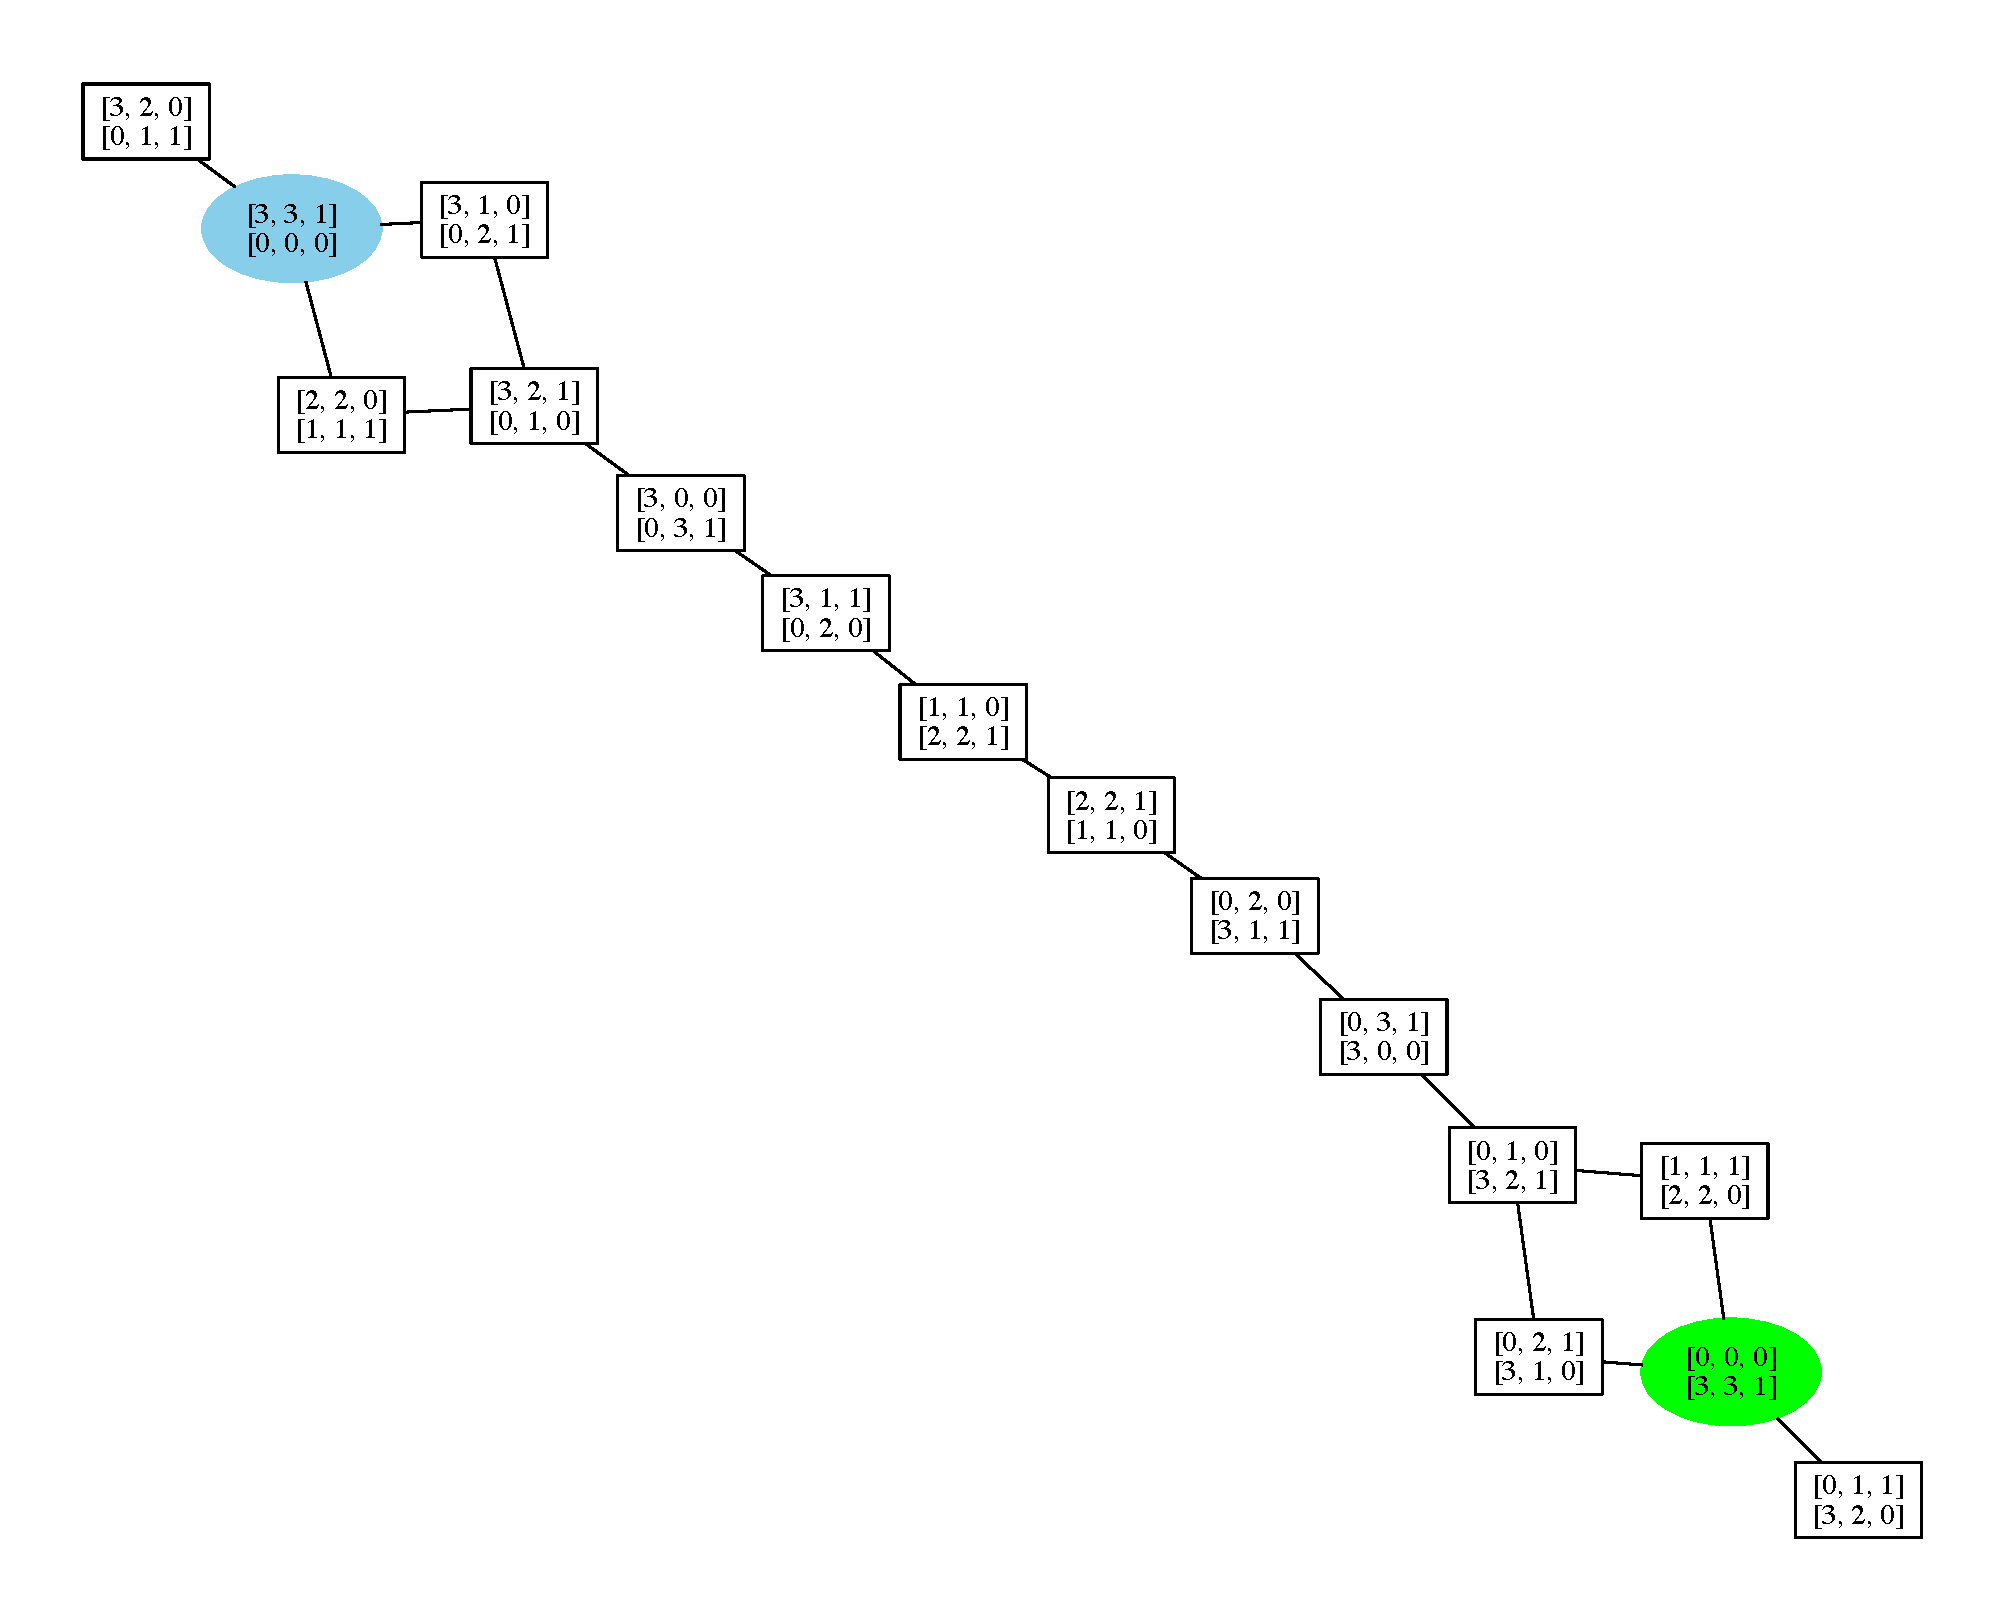
\epsfig{file=Figures/missionare.pdf,scale=0.5}} 
  \caption{A graphical representation of the missionaries and cannibals problem.}
  \label{fig:missionaries.pdf}
\end{figure}


\section{The Sliding Puzzle} 
The $3 \times 3$ sliding puzzle uses a
square board of length 3.  This board is subdivided into $3 \times 3 = 9$ squares of length 1.  Of
these 9 squares, 8 are occupied with square tiles that are numbered from 1 to 8.  One square remains
empty. Figure \ref{fig:8-puzzle.pdf} on page \ref{fig:8-puzzle.pdf} shows two possible states of this
sliding puzzle.  The $4 \times 4$ \href{https://en.wikipedia.org/wiki/15_puzzle}{sliding puzzle}
is similar to the $3 \times 3$ sliding puzzle but it is played on a square board of length 4
instead.  The $4 \times 4$ sliding puzzle is also known as the \emph{\color{blue}15 puzzle}, while the $3 \times 3$ puzzle is
called the \emph{\color{blue}8 puzzle}.

\begin{figure}[!ht]
\centering
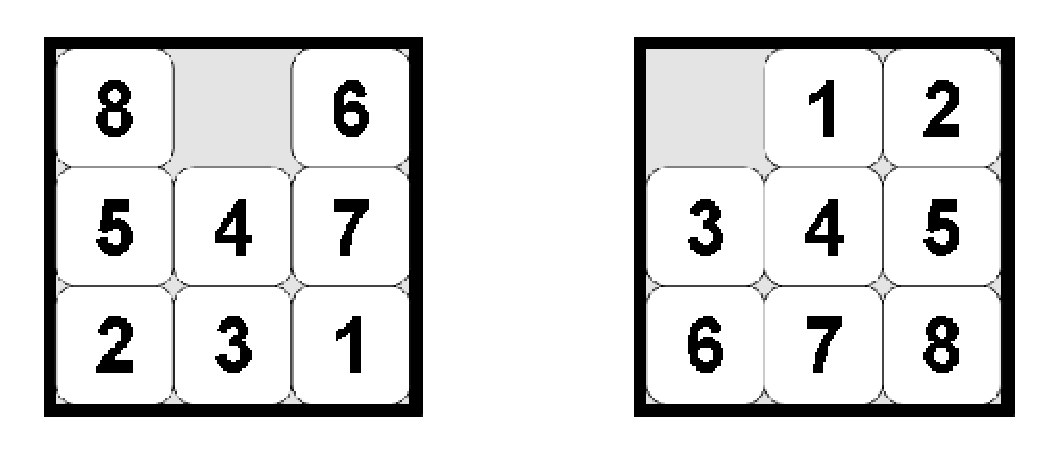
\epsfig{file=Figures/8-puzzle.pdf, scale=0.6}  
\caption{The $3 \times 3$ sliding puzzle.}
\label{fig:8-puzzle.pdf}
\end{figure}

In order to solve the $3 \times 3$ sliding puzzle shown in Figure \ref{fig:8-puzzle.pdf} we have to
transform the state shown on the left of Figure \ref{fig:8-puzzle.pdf} into the state shown on the
right of this figure.  The following operations are permitted when transforming a state of the
sliding puzzle:
\begin{enumerate}
\item If a tile is to the left  of the free square, this tile can be moved to the right.
\item If a tile is to the right of the free square, this tile can be moved to the left.
\item If a tile is above           the free square, this tile can be moved down.
\item If a tile is below           the free square, this tile can be moved up.
\end{enumerate}
In order to get a feeling for the complexity of the sliding puzzle, you can check the page
\\[0.2cm]
\hspace*{1.3cm}
\href{http://mypuzzle.org/sliding}{http://mypuzzle.org/sliding}.
\\[0.2cm]
The sliding puzzle is much more complex than the missionaries and cannibals problem because the
state space is much larger.  For the case of the $3 \times 3$ sliding puzzle, there are 9 squares
that can be positioned in $9!$ different ways.  It turns out that only half of these positions are
reachable from a given start state.  Therefore, the effective number of states for the $3 \times 3$
sliding puzzle is
\\[0.2cm]
\hspace*{1.3cm}
$9! / 2 = 181,440$.
\\[0.2cm]
This is already a big number, but $181,440$ states can still be stored in a modern computer.  However, the
$4 \times 4$ sliding puzzle has
\\[0.2cm]
\hspace*{1.3cm}
$16!/2 = 10,461,394,944,000$
\\[0.2cm]
different states reachable from a given start state.  If a state is represented as matrix containing
16 numbers and we store every number using just 4 bits, we still need $16 \cdot 4 = 64$ bits or 8
bytes for every state.  Hence we would need a total of
\\[0.2cm]
\hspace*{1.3cm}
$(16! / 2) \cdot 8 = 83,691,159,552,000$
\\[0.2cm]
bytes to store every state. We would thus need about 84 Terabytes to store the set of all states.  As few
computers are equipped with this kind of memory, it is obvious that we won't be able to store the
entire state space in memory.

\begin{figure}[!ht]
\centering
\begin{Verbatim}[ frame         = lines, 
                  framesep      = 0.3cm, 
                  firstnumber   = 1,
                  labelposition = bottomline,
                  numbers       = left,
                  numbersep     = -0.2cm,
                  xleftmargin   = 0.8cm,
                  xrightmargin  = 0.8cm,
                ]
    findTile := procedure(number, state) {
        n := #state;
        L := [1 .. n]; 
        for (row in L, col in L | state[row][col] == number) {
            return [row, col];
        }
    };
    moveDir := procedure(state, row, col, dx, dy) {
        state[row     ][col     ] := state[row + dx][col + dy];
        state[row + dx][col + dy] := 0;
        return state;
    };
    nextStates := procedure(state) {
        n          := #state;
        [row, col] := findTile(0, state);
        newStates  := [];
        directions := [ [1, 0], [-1, 0], [0, 1], [0, -1] ];
        L          := [1 .. n];
        for ([dx, dy] in directions) {
            if (row + dx in L && col + dy in L) {
                newStates += [ moveDir(state, row, col, dx, dy) ];
            }
        }
        return newStates;
    };
    start := [ [8, 0, 6],
               [5, 4, 7],
               [2, 3, 1]
             ];
    goal := [ [0, 1, 2], 
              [3, 4, 5], 
              [6, 7, 8]
            ];
\end{Verbatim}
\vspace*{-0.3cm}
\caption{The $3 \times 3$ sliding puzzle.}
\label{fig:sliding-puzzle.stlx}
\end{figure}
Figure \ref{fig:sliding-puzzle.stlx} shows how the $3 \times 3$ sliding puzzle can be formulated as
a search problem.  We discuss this program line by line.
\begin{enumerate}
\item $\mathtt{findTile}$ is an auxiliary procedure that takes a $\mathtt{number}$ and a $\mathtt{state}$ and
      returns the row and column where the tile labelled with $\mathtt{number}$ can be found.  

      Here, a state is represented as a list of lists.  For example, the states shown in Figure
      \ref{fig:8-puzzle.pdf} are represented as shown in line 26 and line 30.  The empty tile is
      coded as $0$. 
\item $\mathtt{moveDir}$ takes a $\mathtt{state}$, the $\mathtt{row}$ and the $\mathtt{col}$umn
      where to find the empty square and a direction in which the empty square should be moved.
      This direction is specified via the two variables $\mathtt{dx}$ and $\mathtt{dy}$.  The tile
      at the position $\langle\mathtt{row} + \mathtt{dx}, \mathtt{col} + \mathtt{dy}\rangle$ is
      moved into the position $\langle\mathtt{row}, \mathtt{col}\rangle$, while the tile at position
      $\langle\mathtt{row} + \mathtt{dx}, \mathtt{col} + \mathtt{dy}\rangle$ becomes empty.
\item Given a $\mathtt{state}$, the procedure $\mathtt{newStates}$ computes the set of all states
      that can be reached in one step from $\mathtt{state}$.  The basic idea is to find the position of the
      empty tile and then try to move the empty tile in all possible directions.  If the empty tile is found at
      position $[\mathtt{row}, \mathtt{col}]$ and the direction of the movement is given as $[\mathtt{dx}, \mathtt{dy}]$, then
      in order to ensure that the empty tile can be moved to the position $[\mathtt{row}+\mathtt{dx}, \mathtt{col}+\mathtt{dy}]$,
      we have to ensure that both
      \\[0.2cm]
      \hspace*{1.3cm}
      $\mathtt{row}+\mathtt{dx} \in \{1,\cdots,n\}$ \quad and \quad
      $\mathtt{col}+\mathtt{dy} \in \{1,\cdots,n\}$
      \\[0.2cm]
      hold, where $n$ is the size of the board.
\end{enumerate}

Next, we want to develop an algorithm that can solve puzzles of the kind described so far.  The most basic
algorithm to solve search problems is \href{https://en.wikipedia.org/wiki/Breadth-first_search}{breadth first search}. 
We discuss this algorithm next.

\section{Breadth First Search}
Informally, breadth first search, abbreviated as \textsc{Bfs}, works as follows:
\begin{enumerate}
\item Given a search problems $\langle Q,\mathtt{nextStates}, \mathtt{start}, \mathtt{goal}\rangle$,  
      we initialize a set $\mathtt{Frontier}$ to contain the state $\mathtt{start}$.

      In general, $\mathtt{Frontier}$ contains those states that have just been discovered and whose successors have not
      yet been seen.
\item As long as the set $\mathtt{Frontier}$ does not contain the state $\mathtt{goal}$, we recompute this set 
      by adding all states to it that can be reached in step from a state in $\mathtt{Frontier}$.
      Then, the states that had been previously present in $\mathtt{Frontier}$ are removed.
      These old states are then saved into a set $\mathtt{Visited}$.
\end{enumerate}
In order to avoid loops, an implementation of breadth first search keeps track of those states that have
been visited.  These states a collected in a set $\mathtt{Visited}$.  Once a state has been added to
the set $\mathtt{Visited}$,  it will never be revisited again. 
Furthermore, in order to keep track of the path leading to the goal, we have a dictionary
$\mathtt{Parent}$.  For every state $s$ that is in $\mathtt{Frontier}$, $\mathtt{Parent}[s]$ is the state that
caused $s$ to be added to the set $\mathtt{Frontier}$, i.e.~we have
\\[0.2cm]
\hspace*{1.3cm}
$s \in \mathtt{nextStates}(\mathtt{Parent}[s])$.


\begin{figure}[!ht]
\centering
\begin{Verbatim}[ frame         = lines, 
                  framesep      = 0.3cm, 
                  firstnumber   = 1,
                  labelposition = bottomline,
                  numbers       = left,
                  numbersep     = -0.2cm,
                  xleftmargin   = 0.8cm,
                  xrightmargin  = 0.8cm,
                ]
    search := procedure(start, goal, nextStates) {
        Frontier := { start };
        Visited  := {}; // set of nodes that have been expanded
        Parent   := {};
        while (Frontier != {}) {
            NewFrontier := {};
            for (s in Frontier, ns in nextStates(s) | !(ns in Visited)) {
                NewFrontier += { ns };
                Parent[ns]  := s;
                if (ns == goal) {
                    return pathTo(goal, Parent);
                }
            }
            Visited  += Frontier;
            Frontier := NewFrontier;
        }
    };
\end{Verbatim}
\vspace*{-0.3cm}
\caption{Breadth first search.}
\label{fig:breadth-first-search.stlx}
\end{figure}
\myFig{breadth-first-search.stlx} shows an implementation of
breadth first search in \textsc{SetlX}.  We discuss this implementation line by line:
\begin{enumerate}
\item $\mathtt{Frontier}$ is the set of all those states that have been encountered but whose
      neighbours have not yet been explored.  Initially, it contains the state $\mathtt{start}$.
\item $\mathtt{Visited}$ is the set of all those states, all whose neighbours have already been
      added to the set $\mathtt{Frontier}$.  In order to avoid infinite loops, these states must not
      be visited again.
\item $\mathtt{Parent}$ is a dictionary keeping track of the state leading to a given state.
\item As long as the set $\mathtt{Frontier}$ is not empty, we add all neighbours of states in 
      $\mathtt{Frontier}$ that have not yet been visited to the set $\mathtt{NewFrontier}$.
      When doing this, we keep track of the path leading to a new state $\mathtt{ns}$ by storing its
      parent in the dictionary $\mathtt{Parent}$.
\item If the new state happens to be the state $\mathtt{goal}$, we return a path leading from
      $\mathtt{start}$ to $\mathtt{goal}$.  The procedure $\mathtt{pathTo}()$ is shown in Figure
      \ref{fig:pathTo.stlx} on page \pageref{fig:pathTo.stlx}.
\item After we have collected all successors of states in $\mathtt{Frontier}$, the states
      in the set $\mathtt{Frontier}$ have been visited and are therefore added to the set
      $\mathtt{Visited}$, while the $\mathtt{Frontier}$ is updated to $\mathtt{NewFrontier}$.
\end{enumerate}

\begin{figure}[!ht]
\centering
\begin{Verbatim}[ frame         = lines, 
                  framesep      = 0.3cm, 
                  firstnumber   = 1,
                  labelposition = bottomline,
                  numbers       = left,
                  numbersep     = -0.2cm,
                  xleftmargin   = 0.8cm,
                  xrightmargin  = 0.8cm,
                ]
    pathTo := procedure(state, Parent) {
        Path := [];
        while (state != om) {
            Path  += [state];
            state := Parent[state];
        }
        return reverse(Path);
    };
\end{Verbatim}
\vspace*{-0.3cm}
\caption{The procedure $\mathtt{pathTo}()$.}
\label{fig:pathTo.stlx}
\end{figure}
The procedure call $\mathtt{pathTo}(\mathtt{state}, \mathtt{Parent})$ constructs a path reaching
from $\mathtt{start}$ to $\mathtt{state}$ in reverse by looking up the parent states.

If we try breadth first search to solve the missionaries and cannibals problem, we immediately get
the solution shown in Figure \ref{fig:missionaries.solution}.  15 nodes had to be expanded to find
this solution.  To keep this in perspective, we note that Figure \ref{fig:missionaries.pdf} shows
that the entire state space contains 16 states.  Therefore, with the exception of one state, we have
inspected all the states.  This is a typical behaviour for breadth first search.

\begin{figure}[!ht]
\centering
\begin{Verbatim}[ frame         = lines, 
                  framesep      = 0.3cm, 
                  firstnumber   = 1,
                  labelposition = bottomline,
                  numbers       = left,
                  numbersep     = -0.2cm,
                  xleftmargin   = 0.8cm,
                  xrightmargin  = 0.8cm,
                ]
    MMM   KKK   B      |~~~~~|                   
                       >  KK >
    MMM   K            |~~~~~|              KK  B
                       <  K  <
    MMM   KK    B      |~~~~~|               K   
                       >  KK >
    MMM                |~~~~~|             KKK  B
                       <  K  <
    MMM   K     B      |~~~~~|              KK   
                       > MM  >
    M     K            |~~~~~|        MM    KK  B
                       < M K <
    MM    KK    B      |~~~~~|         M     K   
                       > MM  >
          KK           |~~~~~|       MMM     K  B
                       <  K  <
          KKK   B      |~~~~~|       MMM         
                       >  KK >
          K            |~~~~~|       MMM    KK  B
                       <  K  <
          KK    B      |~~~~~|       MMM     K   
                       >  KK >
                       |~~~~~|       MMM   KKK  B
\end{Verbatim}
\vspace*{-0.3cm}
\caption{A solution of the missionaries and cannibals problem.}
\label{fig:missionaries.solution}
\end{figure}

Next, let us try to solve the $3 \times 3$ sliding puzzle.  It takes less about 9 seconds to solve
this problem on my computer\footnote{
  I happen to own an iMac from 2011.  This iMac is equipped with 16 Gigabytes of main memory and a
  quad core 2.7 GHz ``Intel Core i5'' processor.  I suspect this to be the I5-2500S (Sandy Bridge) processor.
}, while 181439 states are touched.  Again, we see that breadth first search touches nearly all the
states reachable from the start state.

\subsection{A Queue Based Implementation of Breadth First Search}
In the literature, for example in Figure 3.11 of Russell \& Norvig \cite{russell:2009}, breadth
first search is often implemented using a
\href{https://en.wikipedia.org/wiki/Queue_(abstract_data_type)}{queue} data structure.  
Figure \ref{fig:breadth-first-search-queue.stlx} on page
\pageref{fig:breadth-first-search-queue.stlx} shows an implementation of breadth first search that
uses a queue to store the set \texttt{Frontier}.  However, when we run this version, it turns out
that the solution of the $3 \times 3$ sliding puzzle needs about 58 seconds, which is a lot
slower than our set based implementation that has been presented in Figure
\ref{fig:breadth-first-search.stlx}.

\begin{figure}[!ht]
\centering
\begin{Verbatim}[ frame         = lines, 
                  framesep      = 0.3cm, 
                  firstnumber   = 1,
                  labelposition = bottomline,
                  numbers       = left,
                  numbersep     = -0.2cm,
                  xleftmargin   = 0.8cm,
                  xrightmargin  = 0.8cm,
                ]
    search := procedure(start, goal, nextStates) {
        Queue   := [ start ];
        Visited := {}; 
        Parent  := {};
        while (Queue != []) {
            state := Queue[1];
            Queue := Queue[2..];
            if (state == goal) {
                return pathTo(state, Parent);
            }
            Visited   += { state };
            newStates := nextStates(state);
            for (ns in newStates | !(ns in Visited) && Parent[ns] == om) { 
                Parent[ns] := state;
                Queue      += [ ns ];
            }
        }
    };
\end{Verbatim}
\vspace*{-0.3cm}
\caption{A queue based implementation of breadth first search.}
\label{fig:breadth-first-search-queue.stlx}
\end{figure}

The solution of the $3 \times 3$ sliding puzzle that is found by breadth first search is shown in
Figure \ref{fig:8-puzzle.solution1} and Figure \ref{fig:8-puzzle.solution2}.

\begin{figure}[!ht]
\centering
\begin{Verbatim}[ frame         = lines, 
                  framesep      = 0.3cm, 
                  firstnumber   = 1,
                  labelposition = bottomline,
                  numbers       = left,
                  numbersep     = -0.2cm,
                  xleftmargin   = 0.8cm,
                  xrightmargin  = 0.8cm,
                ]
    +---+---+---+        +---+---+---+        +---+---+---+        +---+---+---+
    | 8 |   | 6 |        |   | 8 | 6 |        | 5 | 8 | 6 |        | 5 | 8 | 6 |
    +---+---+---+        +---+---+---+        +---+---+---+        +---+---+---+
    | 5 | 4 | 7 |  |==>  | 5 | 4 | 7 |  |==>  |   | 4 | 7 |  |==>  | 2 | 4 | 7 |  |==>
    +---+---+---+        +---+---+---+        +---+---+---+        +---+---+---+
    | 2 | 3 | 1 |        | 2 | 3 | 1 |        | 2 | 3 | 1 |        |   | 3 | 1 |
    +---+---+---+        +---+---+---+        +---+---+---+        +---+---+---+

    +---+---+---+        +---+---+---+        +---+---+---+        +---+---+---+
    | 5 | 8 | 6 |        | 5 | 8 | 6 |        | 5 | 8 | 6 |        | 5 | 8 |   |
    +---+---+---+        +---+---+---+        +---+---+---+        +---+---+---+
    | 2 | 4 | 7 |  |==>  | 2 | 4 | 7 |  |==>  | 2 | 4 |   |  |==>  | 2 | 4 | 6 |  |==>
    +---+---+---+        +---+---+---+        +---+---+---+        +---+---+---+
    | 3 |   | 1 |        | 3 | 1 |   |        | 3 | 1 | 7 |        | 3 | 1 | 7 |
    +---+---+---+        +---+---+---+        +---+---+---+        +---+---+---+

    +---+---+---+        +---+---+---+        +---+---+---+        +---+---+---+
    | 5 |   | 8 |        |   | 5 | 8 |        | 2 | 5 | 8 |        | 2 | 5 | 8 |
    +---+---+---+        +---+---+---+        +---+---+---+        +---+---+---+
    | 2 | 4 | 6 |  |==>  | 2 | 4 | 6 |  |==>  |   | 4 | 6 |  |==>  | 4 |   | 6 |  |==>
    +---+---+---+        +---+---+---+        +---+---+---+        +---+---+---+
    | 3 | 1 | 7 |        | 3 | 1 | 7 |        | 3 | 1 | 7 |        | 3 | 1 | 7 |
    +---+---+---+        +---+---+---+        +---+---+---+        +---+---+---+

    +---+---+---+        +---+---+---+        +---+---+---+        +---+---+---+
    | 2 | 5 | 8 |        | 2 | 5 | 8 |        | 2 | 5 | 8 |        | 2 | 5 |   |
    +---+---+---+        +---+---+---+        +---+---+---+        +---+---+---+
    | 4 | 1 | 6 |  |==>  | 4 | 1 | 6 |  |==>  | 4 | 1 |   |  |==>  | 4 | 1 | 8 |  |==>
    +---+---+---+        +---+---+---+        +---+---+---+        +---+---+---+
    | 3 |   | 7 |        | 3 | 7 |   |        | 3 | 7 | 6 |        | 3 | 7 | 6 |
    +---+---+---+        +---+---+---+        +---+---+---+        +---+---+---+

    +---+---+---+        +---+---+---+        +---+---+---+        +---+---+---+        
    | 2 |   | 5 |        |   | 2 | 5 |        | 4 | 2 | 5 |        | 4 | 2 | 5 |
    +---+---+---+        +---+---+---+        +---+---+---+        +---+---+---+
    | 4 | 1 | 8 |  |==>  | 4 | 1 | 8 |  |==>  |   | 1 | 8 |  |==>  | 1 |   | 8 |  |==>
    +---+---+---+        +---+---+---+        +---+---+---+        +---+---+---+
    | 3 | 7 | 6 |        | 3 | 7 | 6 |        | 3 | 7 | 6 |        | 3 | 7 | 6 |
    +---+---+---+        +---+---+---+        +---+---+---+        +---+---+---+

    +---+---+---+        +---+---+---+        +---+---+---+        +---+---+---+        
    | 4 | 2 | 5 |        | 4 | 2 | 5 |        | 4 | 2 | 5 |        | 4 | 2 |   |
    +---+---+---+        +---+---+---+        +---+---+---+        +---+---+---+
    | 1 | 7 | 8 |  |==>  | 1 | 7 | 8 |  |==>  | 1 | 7 |   |  |==>  | 1 | 7 | 5 |  |==>
    +---+---+---+        +---+---+---+        +---+---+---+        +---+---+---+
    | 3 |   | 6 |        | 3 | 6 |   |        | 3 | 6 | 8 |        | 3 | 6 | 8 |
    +---+---+---+        +---+---+---+        +---+---+---+        +---+---+---+
\end{Verbatim}
\vspace*{-0.3cm}
\caption{The first 24 steps in the solution of the $3 \times 3$ sliding puzzle.}
\label{fig:8-puzzle.solution1}
\end{figure}

\begin{figure}[!ht]
\centering
\begin{Verbatim}[ frame         = lines, 
                  framesep      = 0.3cm, 
                  firstnumber   = 1,
                  labelposition = bottomline,
                  numbers       = left,
                  numbersep     = -0.2cm,
                  xleftmargin   = 0.8cm,
                  xrightmargin  = 0.8cm,
                ]
    +---+---+---+        +---+---+---+        +---+---+---+        +---+---+---+        
    | 4 |   | 2 |        |   | 4 | 2 |        | 1 | 4 | 2 |        | 1 | 4 | 2 |
    +---+---+---+        +---+---+---+        +---+---+---+        +---+---+---+
    | 1 | 7 | 5 |  |==>  | 1 | 7 | 5 |  |==>  |   | 7 | 5 |  |==>  | 3 | 7 | 5 |  |==>
    +---+---+---+        +---+---+---+        +---+---+---+        +---+---+---+
    | 3 | 6 | 8 |        | 3 | 6 | 8 |        | 3 | 6 | 8 |        |   | 6 | 8 |
    +---+---+---+        +---+---+---+        +---+---+---+        +---+---+---+

    +---+---+---+        +---+---+---+        +---+---+---+        +---+---+---+        
    | 1 | 4 | 2 |        | 1 | 4 | 2 |        | 1 |   | 2 |        |   | 1 | 2 |
    +---+---+---+        +---+---+---+        +---+---+---+        +---+---+---+
    | 3 | 7 | 5 |  |==>  | 3 |   | 5 |  |==>  | 3 | 4 | 5 |  |==>  | 3 | 4 | 5 |  
    +---+---+---+        +---+---+---+        +---+---+---+        +---+---+---+
    | 6 |   | 8 |        | 6 | 7 | 8 |        | 6 | 7 | 8 |        | 6 | 7 | 8 |
    +---+---+---+        +---+---+---+        +---+---+---+        +---+---+---+
\end{Verbatim}
\vspace*{-0.3cm}
\caption{The last 7 steps in the solution of the $3 \times 3$ sliding puzzle.}
\label{fig:8-puzzle.solution2}
\end{figure}

We conclude our discussion of breadth first search by noting the two most important properties of
breadth first search.
\begin{enumerate}
\item Breadth first search is \emph{\color{blue}complete}:  If there is a solution to the given
      search problem, then breadth first search is going to find it.
\item The solution found by breadth first search is \emph{\color{blue}optimal}, i.e.~it is the
      shortest possible solution.
\end{enumerate}
\proof
Both of these claims can be shown simultaneously.  Consider the implementation of breadth first
search shown in Figure \ref{fig:breadth-first-search.stlx}.  An easy induction on the number of
iterations of the \texttt{while} loop shows that after $n$ iterations of the \texttt{while} loop,
the set $\mathtt{Frontier}$ contains exactly those states that have a distance of $n$ to the state 
$\mathtt{start}$.  This claim is obviously true before the first iteration of the while loop as in
this case, $\mathtt{Frontier}$ only contains the state $\mathtt{start}$.  In the induction step we
assume the claim is true after $n$ iterations.  Then, in the next iteration all states that can be
reached in one step from a state in $\mathtt{Frontier}$ are added to the new $\mathtt{Frontier}$,
provided there is no shorter path to these states.  There is a shorter path to these states if these
states are already a member of the set $\mathtt{Visited}$.  Hence, the claim is true after $n+1$
iterations also.

Now, if there is a path form $\mathtt{start}$ to $\mathtt{goal}$, there must also be a shortest
path.  Assume this path has a length of $k$.  Then, $\mathtt{goal}$ is reached in the iteration
number $k$ and the shortest path is returned.
\qed

The fact that breadth first search is both complete and the path returned is optimal is rather
satisfying.  However, breadth first search still has a big downside that makes it unusable for
many problems:  If the \texttt{goal} is far from the $\mathtt{start}$, breadth first search will use
a lot of memory because it will store a large part of the state space in the set
$\mathtt{Visited}$.  In many cases, the state space is so big that this is not possible.  For example, it is
impossible to solve the more interesting cases of the $4 \times 4$ sliding puzzle.
\pagebreak


\section{Depth First Search}
To overcome the memory limitations of breadth first search, the
\href{https://en.wikipedia.org/wiki/Depth-first_search}{depth first search} algorithm has been
developed.  The basic idea is to replace the queue of Figure
\ref{fig:breadth-first-search-queue.stlx} by a stack.  The resulting algorithm is shown in Figure
\ref{fig:depth-first-search.stlx} on page \pageref{fig:depth-first-search.stlx}.  Basically, in this
implementation, a path is searched to its end before trying an alternative.  This way, we might be able to find a
$\mathtt{goal}$ that is far away from $\mathtt{start}$ without exploring the whole state space.  

\begin{figure}[!ht]
\centering
\begin{Verbatim}[ frame         = lines, 
                  framesep      = 0.3cm, 
                  firstnumber   = 1,
                  labelposition = bottomline,
                  numbers       = left,
                  numbersep     = -0.2cm,
                  xleftmargin   = 0.8cm,
                  xrightmargin  = 0.8cm,
                ]
    search := procedure(start, goal, nextStates) {
        Stack  := [ start ];
        Parent := {};
        while (Stack != []) {
            state := Stack[-1];
            Stack := Stack[..-2];
            if (state == goal) {
                return pathTo(state, Parent);
            }
            newStates := nextStates(state);
            for (ns in newStates | ns != start && Parent[ns] == om) { 
                Parent[ns] := state;
                Stack      += [ns];
            }
        }
    };
\end{Verbatim}
\vspace*{-0.3cm}
\caption{The depth first search algorithm.}
\label{fig:depth-first-search.stlx}
\end{figure}
Actually, it is not necessary to understand the details of the implementation shown in
\myFig{depth-first-search.stlx}.  The reason is that the recursive implementation of depth first
search that is presented in the following subsection is superior to the implementation shown in
\myFig{depth-first-search.stlx}.
When we test the implementation shown above with the $3 \times 3$ sliding puzzle, it takes about 96 seconds to find a solution.  
The solution that is found has a length of $41,553$ steps.  As the
shortest path from $\mathtt{start}$ to $\mathtt{goal}$ has 31 steps, the solution found by depth
first search is very far from optimal.  All this is rather disappointing news.  The only good news
is that there is no longer a need to keep the set $\mathtt{Visited}$ around.  However, we still have
to maintain the set $\mathtt{Parent}$.  If we were more ambitious, we could eliminate the use of
this dictionary also, but the resulting implementation would be rather unwieldy.  Fortunately, we will be
able to get rid of the set $\mathtt{Parent}$ with next to no effort when we develop a recursive
implementation of depth first search in the following subsection.

\subsection{Getting Rid of the $\mathtt{Parent}$ Dictionary}
It can be argued that the implementation of depth first search discussed previously is not really
depth first search because it uses the dictionary $\mathtt{Parent}$.  As states are only added to
$\mathtt{Parent}$ and never removed, at the end of the search this dictionary will contain all
states that have been visited.  This defeats the most important advantage of depth first search
which is the fact that it should only store the current path that is investigated.  Therefore,
it has been suggested (for example compare Russel and Norvig \cite{russell:2009}) that instead of
storing single states, the stack should store the full paths leading to these states.  This leads to
the implementation shown in \myFig{depth-first-search-path.stlx}. 

\begin{figure}[!ht]
\centering
\begin{Verbatim}[ frame         = lines, 
                  framesep      = 0.3cm, 
                  firstnumber   = 1,
                  labelposition = bottomline,
                  numbers       = left,
                  numbersep     = -0.2cm,
                  xleftmargin   = 0.8cm,
                  xrightmargin  = 0.8cm,
                ]
    search := procedure(start, goal, nextStates) {
        Stack  := [ [start] ];
        while (Stack != []) {
            Path  := Stack[-1];
            Stack := Stack[..-2];
            state := Path[-1];
            if (state == goal) {
                return Path;
            }
            newStates := nextStates(state);
            for (ns in newStates | !(ns in Path)) { 
                Stack += [ Path + [ns] ];
            }
        }
    };
\end{Verbatim}
\vspace*{-0.3cm}
\caption{An path-based implementation of depth first search.}
\label{fig:depth-first-search-path.stlx}
\end{figure}

Unfortunately, it  turns out that the paths get very long and hence need a lot of memory to be
stored and this fact defeats the main idea of this implementation.  As a result, the procedure
$\mathtt{search}$ that is given in \myFig{depth-first-search-path.stlx} is not able to solve the
instance of the  $3 \times 3$ sliding puzzle that was shown in \myFig{8-puzzle.pdf}.

\exercise
Assume the set of states $Q$ is defined as
\\[0.2cm]
\hspace*{1.3cm}
$Q := \bigl\{ \pair(a, b) \mid a \in \mathbb{N} \wedge b \in \mathbb{N} \bigr\}$.
\\[0.2cm]
Furthermore, the states $\mathtt{start}$ and $\mathtt{goal}$ are defined as
\\[0.2cm]
\hspace*{1.3cm}
$\mathtt{start} := \pair(0,0)$ \quad and \quad $\mathtt{goal} := \pair(n,0)$ where $n \in \mathbb{N}$.
\\[0.2cm]
Next, the function $\mathtt{nextStates}$ is defined as
\\[0.2cm]
\hspace*{1.3cm}
$\mathtt{nextStates}\bigl(\pair(a,b)\bigr) := \bigl\{\pair(a+1,b), \pair(a,b+1)\bigr\}$.
\\[0.2cm]
Finally, the search problem $\mathcal{P}$ is defined as
\\[0.2cm]
\hspace*{1.3cm}
$\mathcal{P} := \langle Q, \mathtt{nextStates}, \mathtt{start}, \mathtt{goal} \rangle$.
\\[0.2cm]
Assume that states can be stored using 8 bytes.  Furthermore, assume that we use the algorithm given in
\myFig{depth-first-search-path.stlx} to solve the search problem $\mathcal{P}$.
How many bytes do we need to store all the states on the stack in the moment that the $\mathtt{goal}$
is reached? How big is this number if $n = 10,000$?
\vspace*{0.2cm}

\noindent
\begin{enumerate}[(a)]
\item \textbf{Note} that the question only asks for the memory needed to store the states.  The memory
      needed to store the stack itself and the various lists on the stack comes on top of the memory
      needed to store the states.  However,
      to answer this exercise correctly, you should ignore this type of memory.
\item In order to understand how the stack evolves, we need to know that in \textsc{SetlX} sets are ordered
      ascendingly.  Furthermore, pairs are ordered lexicographically in \textsc{SetlX}, i.e. we have
      \\[0.2cm]
      \hspace*{1.3cm}
      $\pair(x_1, y_1) < \pair(x_2, y_2) \quad\Longleftrightarrow\quad x_1 < x_2 \vee (x_1 = x_2 \wedge y_1 < y_2)$.
      \\[0.2cm]
      Hence, when we have a state $\pair(a, b)$, the set $\mathtt{nextStates}\bigl(\pair(a, b)\bigr)$ is
      ordered as follows:
      \\[0.2cm]
      \hspace*{1.3cm}
      $\bigl\{\pair(a,b+1)\bigr\}, \pair(a+1,b) \bigr\}$. \eoxs
\end{enumerate}

\subsection{A Recursive Implementation of Depth First Search}
Sometimes, the depth first search algorithm is presented as a recursive algorithm, since this leads
to an implementation that is slightly shorter and more easy to understand.  What is more, we no
longer need the dictionary $\mathtt{Parent}$ to record the parent of each node.  The resulting
implementation is shown in \myFig{depth-first-search-recursive.stlx}.

\begin{figure}[!ht]
\centering
\begin{Verbatim}[ frame         = lines, 
                  framesep      = 0.3cm, 
                  firstnumber   = 1,
                  labelposition = bottomline,
                  numbers       = left,
                  numbersep     = -0.2cm,
                  xleftmargin   = 0.8cm,
                  xrightmargin  = 0.8cm,
                ]
    search := procedure(start, goal, nextStates) {
        return dfs(start, goal, nextStates, [start]);
    };    
    dfs := procedure(state, goal, nextStates, Path) {
        if (state == goal) {
            return Path;
        }
        newStates := nextStates(state);
        for (ns in newStates | !(ns in Path)) {
            result     := dfs(ns, goal, nextStates, Path + [ns]);
            if (result != om) {
                return result;
            }   
        }
    };
\end{Verbatim}
\vspace*{-0.3cm}
\caption{A recursive implementation of depth first search.}
\label{fig:depth-first-search-recursive.stlx}
\end{figure}
The only purpose of the procedure \texttt{search} is to call the procedure $\mathtt{dfs}$, which needs one
additional argument.  This argument is called $\mathtt{Path}$.  The idea is that $\mathtt{Path}$ is
a path leading from the state $\mathtt{start}$ to the current $\mathtt{state}$ that is the first
argument of the procedure $\mathtt{dfs}$.  Of course, on the first invocation of $\mathtt{dfs}$, the
parameter $\mathtt{state}$ is equal to $\mathtt{start}$ and therefore $\mathtt{Path}$ is initialized
as the list containing only $\mathtt{start}$.

The implementation of $\mathtt{dfs}$ works as follows:
\begin{enumerate}
\item If $\mathtt{state}$ is equal to $\mathtt{goal}$, our search is successful. Since by assumption
      the list $\mathtt{Path}$ is a path connecting $\mathtt{start}$ and $\mathtt{state}$ and we
      have checked that $\mathtt{state}$ is equal to $\mathtt{goal}$, we can return $\mathtt{Path}$ as our solution.
\item Otherwise, $\mathtt{newStates}$ is the set of states that are reachable from $\mathtt{state}$
      in one step.  Any of the states $\mathtt{ns}$ in this set could be the next state on a path
      that leads to $\mathtt{goal}$.  Therefore, we try recursively to reach $\mathtt{goal}$ from
      every state $\mathtt{ns}$.  Note that we have to change $\mathtt{Path}$ to the list
      \\[0.2cm]
      \hspace*{1.3cm}
      \texttt{Path + [ns]}
      \\[0.2cm]
      when we call the procedure $\mathtt{dfs}$ recursively.  This way, we retain the invariant of
      $\mathtt{dfs}$ that the list $\mathtt{Path}$ is a path connecting $\mathtt{start}$ with $\mathtt{state}$.
\item We still have to avoid running in circles.  In the recursive version of depth first search, 
      this is achieved by checking that the state $\mathtt{ns}$ is not already a member of the list $\mathtt{Path}$.  In the
      non-recursive version of depth first search, we had used the set $\mathtt{Parent}$ instead.
      The current implementation no longer has a need for the dictionary $\mathtt{Parent}$.  This is very 
      fortunate since it reduces the memory requirements of depth first search considerably.
\item If one of the recursive calls of $\mathtt{dfs}$ returns a list, this list is a solution to our
      search problem and hence it is returned.  However, if instead the undefined value
      $\mathtt{om}$ is returned, the \texttt{for} loop needs to carry on and test the other
      successors of $\mathtt{state}$.
\item Note that the recursive invocation of $\mathtt{dfs}$ returns $\mathtt{om}$ if the end of the
      \texttt{for} loop is reached and no solution has been returned so far.  The reason is that there is
      no \texttt{return} statement at the end of the procedure $\mathtt{dfs}$.  Hence, if the last
      line of the procedure $\mathtt{dfs}$ is reached, $\mathtt{om}$ is returned by default.
\end{enumerate}

For the $3 \times 3$ puzzle, it takes about 2 seconds to compute the solution.  In this case, the length of
the solution is still 3653 steps, which is unsatisfying.  The good news is that this program does not
need much memory.  The only variable that uses considerable memory is the variable $\mathtt{Path}$.
If we can somehow keep the list $\mathtt{Path}$ short, then the recursive version of depth first search uses only a
tiny fraction of the memory needed by breadth first search.

\section{Iterative Deepening}
The fact that the recursive version of depth first search took just 2 seconds to find a solution is
very impressive.  The questions is whether it might be possible to force depth first search to find
the shortest solution.  The answer to this question leads to an algorithm that is known as
\href{https://en.wikipedia.org/wiki/Iterative_deepening_depth-first_search}{iterative deepening}.  The main
idea behind iterative deepening is to run depth first with a \emph{\color{blue}depth limit} $d$.  This limit
enforces that a solution has at most a length of $d$.  If no solution is found at a depth of $d$, the new depth
$d+1$ can be tried next and the process can be continued until a solution is found.  The program shown in
Figure \ref{fig:iterative-deepening.stlx} on page \pageref{fig:iterative-deepening.stlx} implements this strategy.
We proceed to discuss the details of this program.

\begin{figure}[!ht]
\centering
\begin{Verbatim}[ frame         = lines, 
                  framesep      = 0.3cm, 
                  firstnumber   = 1,
                  labelposition = bottomline,
                  numbers       = left,
                  numbersep     = -0.2cm,
                  xleftmargin   = 0.8cm,
                  xrightmargin  = 0.8cm,
                ]
    search := procedure(start, goal, nextStates) {
        limit := 1;
        while (true) {
            Path := depthLimitedSearch(start, goal, nextStates, limit);
            if (Path != om) { return Path; }
            limit += 1;
        }
    };
    depthLimitedSearch := procedure(start, goal, nextStates, limit) {
        Stack := [ [start] ];
        while (Stack != []) {
            Path  := Stack[-1];
            Stack := Stack[..-2];
            state := Path[-1];
            if (state == goal)  { return Path; }
            if (#Path >= limit) { continue;    }
            for (ns in nextStates(state) | !(ns in Path)) {  
                Stack += [ Path + [ns] ];
            }
        }
    };
\end{Verbatim}
\vspace*{-0.3cm}
\caption{Iterative deepening implemented in \textsc{SetlX}.}
\label{fig:iterative-deepening.stlx}
\end{figure}

\begin{enumerate}
\item The procedure $\mathtt{search}$ initializes the variable $\mathtt{limit}$ to 1 and tries to find a solution
      to the search problem that has a length that is less than or equal to $\mathtt{limit}$.  If a solution is
      found, it is returned.  Otherwise, the variable $\mathtt{limit}$ is incremented by one and a
      new instance of depth first search is started.  This process continues until either 
      \begin{itemize}
      \item a solution is found \qquad or 
      \item the sun rises in the west. 
      \end{itemize}
\item The procedure $\mathtt{depthLimitedSearch}$ implements depth first search but takes care to compute only
      those paths that have a length of at most $\mathtt{limit}$.  The implementation shown in Figure
      \ref{fig:iterative-deepening.stlx} is stack based.  In this implementation,
      the stack contains paths leading from $\mathtt{start}$ to the state at the end of a given
      path.  Hence it is similar to the implementation of depth first search shown in
      \myFig{depth-first-search.stlx}. 
\item The stack is initialized to contain the path $\mathtt{[start]}$.
\item In the \texttt{while}-loop, the first thing that happens is that the $\mathtt{Path}$ on top of
      the stack is removed from the stack.  The state at the end of this $\mathtt{Path}$ is called $\mathtt{state}$.
      If this $\mathtt{state}$ happens to be the $\mathtt{goal}$, a solution to the search problem
      has been found and this solution is returned.
\item Otherwise, we check the length of $\mathtt{Path}$.  If this length is greater than or equal to the
      $\mathtt{limit}$, the $\mathtt{Path}$ can be discarded as we have already checked that it
      does not end in the $\mathtt{goal}$.
\item Otherwise, the neighbours of $\mathtt{state}$ are computed.  For every neighbour $\mathtt{ns}$
      of $\mathtt{state}$ that has not yet been encountered in $\mathtt{Path}$, we extend
      $\mathtt{Path}$ to a new list that ends in $\mathtt{ns}$.
\item This process is iterated until the $\mathtt{Stack}$ is exhausted.
\end{enumerate}
The nice thing about the program presented in this section is the fact that it does not use much
memory.  The reason is that the stack can never have a size that is longer than $\mathtt{limit}$ and
therefore the overall memory that is needed can be bounded by $\mathcal{O}(\mathtt{limit}^2)$.
However, when we run this program to solve the $3 \times 3$ sliding puzzle, the algorithm takes
about 42 minutes.  There are two reasons for this:
\begin{enumerate}
\item First, it is quite wasteful to run the search for a depth limit of $1$, $2$, $3$, $\cdots$ all the way up
      to 31.  Essentially, all the computations done with a limit less than $31$ are essentially wasted.
\item Given a state $s$ that is reachable from the $\mathtt{start}$, there often is a huge number of
      different paths that lead from start to $s$.  The version of iterative deepening presented in
      this section tries all of these paths and hence needs a large amount of time.
\end{enumerate}

\exercise
Assume the set of states $Q$ is defined as
\\[0.2cm]
\hspace*{1.3cm}
$Q := \bigl\{ \pair(a, b) \mid a \in \mathbb{N} \wedge b \in \mathbb{N} \bigr\}$.
\\[0.2cm]
Furthermore, the states $\mathtt{start}$ and $\mathtt{goal}$ are defined as
\\[0.2cm]
\hspace*{1.3cm}
$\mathtt{start} := \pair(0,0)$ \quad and \quad $\mathtt{goal} := \pair(n,n)$ where $n \in \mathbb{N}$.
\\[0.2cm]
Next, the function $\mathtt{nextStates}$ is defined as
\\[0.2cm]
\hspace*{1.3cm}
$\mathtt{nextStates}\bigl(\pair(a,b)\bigr) := \bigl\{\pair(a+1,b), \pair(a,b+1)\bigr\}$.
\\[0.2cm]
Finally, the search problem $\mathcal{P}$ is defined as
\\[0.2cm]
\hspace*{1.3cm}
$\mathcal{P} := \langle Q, \mathtt{nextStates}, \mathtt{start}, \mathtt{goal} \rangle$.
\\[0.2cm]
Given a natural number $n$, compute the number of different solutions of this search problem and prove
your claim.
\eoxs

\exercise 
If there is no solution, the implementation of iterative deepening that is shown in Figure
\ref{fig:iterative-deepening.stlx} does not terminate.  The reason is that the function $\mathtt{depthLimitedSearch}$ does not
distinguish between the following two reasons for failure:
\begin{enumerate}
\item It can fail to find a solution because the depth limit is reached.
\item It can also fail it has tried all paths without hitting the depth limit but the $\mathtt{Stack}$ is exhausted.  
\end{enumerate}
Improve the implementation of iterative deepening so that it will always terminate eventually, provided the
state space is finite. 
\eoxs

\subsection{A Recursive Implementation of Iterative Deepening}
If we implement iterative deepening recursively, then we know that the call stack is bounded by the length of
the shortest solution.  \myFig{iterative-deepening-recursive.stlx}  
shows a recursive implementation of iterative deepening.  This implementation has several nice features:


\begin{figure}[!ht]
\centering
\begin{Verbatim}[ frame         = lines, 
                  framesep      = 0.3cm, 
                  firstnumber   = 1,
                  labelposition = bottomline,
                  numbers       = left,
                  numbersep     = -0.2cm,
                  xleftmargin   = 0.8cm,
                  xrightmargin  = 0.8cm,
                ]
    search := procedure(start, goal, nextStates) {
        limit := 1;  
        while (true) {
            result := dfsLimited(start, goal, nextStates, [start], limit);
            if (result != om) {
                return result;
            }
            limit += 1;
        }
    };
    dfsLimited := procedure(state, goal, nextStates, Path, limit) {
        if (state == goal) {
            return Path;
        }
        if (limit == 0) {
            return;  // limit execceded
        }
        for (ns in nextStates(state) | !(ns in Path)) {
            result := dfsLimited(ns, goal, nextStates, Path + [ns], limit - 1);
            if (result != om) {
                return result;
            }   
        }
    };
\end{Verbatim}
\vspace*{-0.3cm}
\caption{A recursive implementation of iterative deepening.}
\label{fig:iterative-deepening-recursive.stlx}
\end{figure}
\begin{enumerate}
\item The path that is computed no longer requires the dictionary $\mathtt{Parent}$ as it is built
      incrementally in the argument $\mathtt{Path}$ of the procedure $\mathtt{dfsLimited}$.
\item Similarly, there is no longer a need to keep the dictionary $\mathtt{Distance}$.
\end{enumerate}
Unfortunately, the running time of the recursive implementation of iterative deepening is still
quite big:  On my computer, the recursive implementation takes about 36 minutes.

\section{Bidirectional Breadth First Search}
Breadth first search first visits all states that have a distance of 1 from start, then all
states that have a distance of 2, then of 3 and so on until finally the goal is found.  If the shortest path
from $\mathtt{start}$ to $\mathtt{goal}$ is $d$, then all states that have a distance of at most $d$ will be
visited.  In many search problems, the number of states grows exponentially with the distance, i.e.~there is
a \emph{\color{blue}branching factor} $b$ such that the set of all states that have a distance of at most $d$
from $\mathtt{start}$ is roughly
\\[0.2cm]
\hspace*{1.3cm}
 $\ds 1 + b + b^2 + b^3 + \cdots + b^d = \frac{b^{d+1} - 1}{b - 1} = \mathcal{O}\bigl(b^d\bigr)$. 
\\[0.2cm]
At least this is true in the beginning of the search.  As the size of
the memory that is needed is the most constraining factor when searching, it is important to cut down this
size.  On simple idea is to start searching both from the node $\mathtt{start}$ and the node $\mathtt{goal}$
simultaneously.  The justification is that we can hope that the path starting form $\mathtt{start}$ and the
path starting from $\mathtt{goal}$ will meet in the middle and hence they will both have a size of approximately
$d/2$.  If this is the case, only
\\[0.2cm]
\hspace*{1.3cm}
$\ds 2 \cdot \frac{b^{d/2} - 1}{b - 1}$ 
\\[0.2cm]
nodes need to be explored and even for modest values of $b$ this number is much smaller than 
\\[0.2cm]
\hspace*{1.3cm}
$\ds\frac{b^{d+1} - 1}{b - 1}$
\\[0.2cm]
which is the number of nodes expanded in breadth first search.  For example, assume that the branching factor
$b = 2$ and that the length of the shortest path leading from $\mathtt{start}$ to $\mathtt{goal}$
is $40$.  Then we need to explore
\\[0.2cm]
\hspace*{1.3cm}
$2^{40} - 1 = 1,099,511,627,775$
\\[0.2cm]
in breadth first search, while we only have to explore 
\\[0.2cm]
\hspace*{1.3cm}
$2^{40/2} - 1 = 1,048,575$
\\[0.2cm]
with bidirectional depth first search.  While it is certainly feasible to keep a million states in memory,
keeping a trillion states in memory is impossible on most devices.


\begin{figure}[!ht]
\centering
\begin{Verbatim}[ frame         = lines, 
                  framesep      = 0.3cm, 
                  firstnumber   = 1,
                  labelposition = bottomline,
                  numbers       = left,
                  numbersep     = -0.2cm,
                  xleftmargin   = 0.8cm,
                  xrightmargin  = 0.8cm,
                ]
    search := procedure(start, goal, nextStates) {
        FrontierA := { start };
        VisitedA  := {}; // set of nodes expanded starting from start
        ParentA   := {};
        FrontierB := { goal };
        VisitedB  := {}; // set of nodes expanded starting from goal
        ParentB   := {};
        while (FrontierA != {} && FrontierB != {}) {
            VisitedA += FrontierA;
            VisitedB += FrontierB;
            NewFrontier := {};
            for (s in FrontierA, ns in nextStates(s) | !(ns in VisitedA)) {
                NewFrontier += { ns };
                ParentA[ns] := s;
                if (ns in VisitedB) {
                    return combinePaths(ns, ParentA, ParentB);
                }
            }
            FrontierA   := NewFrontier;
            NewFrontier := {};
            for (s in FrontierB, ns in nextStates(s) | !(ns in VisitedB)) {
                NewFrontier += { ns };
                ParentB[ns] := s;
                if (ns in VisitedA) {
                    return combinePaths(ns, ParentA, ParentB);
                }
            }
            FrontierB := NewFrontier;
        }
    };
\end{Verbatim}
\vspace*{-0.3cm}
\caption{Bidirectional breadth first search.}
\label{fig:bidirectional-bfs.stlx}
\end{figure}

Figure \ref{fig:bidirectional-bfs.stlx} on page \pageref{fig:bidirectional-bfs.stlx} shows the implementation
of bidirectional breadth first search.  Essentially, we have to copy the breadth first program shown in
Figure \ref{fig:breadth-first-search.stlx}. Let us discuss the details of the implementation.
\begin{enumerate}
\item The variable $\mathtt{FrontierA}$ is the frontier that starts from the state $\mathtt{start}$, while
      $\mathtt{FrontierB}$ is the frontier that starts from the state $\mathtt{goal}$.
\item $\mathtt{VisitedA}$ is the set of states that have been visited starting from $\mathtt{start}$, while
      $\mathtt{VisitedB}$ is the set of states that have been visited starting from $\mathtt{goal}$.
\item For every state $s$ that is in $\mathtt{FrontierA}$, $\mathtt{ParentA}[s]$ is the state that caused $s$
      to be added to the set $\mathtt{FrontierA}$.  Similarly, for every state $s$ that is in $\mathtt{FrontierB}$,
      $\mathtt{ParentB}[s]$ is the state that caused $s$ to be added to the set $\mathtt{FrontierB}$.  
\item The bidirectional search keeps running for as long as both sets $\mathtt{FrontierA}$ and
      $\mathtt{FrontierB}$ are non-empty and a path has not yet been found.
\item Initially, the \texttt{while} loop adds the frontier sets to the visited sets
      as all the neighbours of the frontier sets will now be explored.
\item Then the \texttt{while} loop computes those states that can be reached from $\mathtt{FrontierA}$ and have not been
      visited from $\mathtt{start}$.  If a state $\mathtt{ns}$ is a neighbour of a state $\mathtt{s}$ from the set 
      $\mathtt{FrontierA}$ and the state $\mathtt{ns}$ has already been encountered during the search that started
      from $\mathtt{goal}$, then a path leading from $\mathtt{start}$ to $\mathtt{goal}$ has been found and this path
      is returned.  The function \texttt{combinePaths} that computes this path by combining the path that leads
      from $\mathtt{start}$ to $\mathtt{ns}$ and then from $\mathtt{ns}$ to $\mathtt{goal}$ to is shown in Figure
      \ref{fig:combine-paths.stlx} on page \pageref{fig:combine-paths.stlx}.
\item Next, the same computation is done with the role of the states $\mathtt{start}$ and $\mathtt{goal}$ exchanged.
\end{enumerate}
On my computer, bidirectional breadth first search solves the $3 \times 3$ sliding puzzle in less than a
second!  However, bidirectional breadth first search is still not able to solve the $4 \times 4$ sliding puzzle
since the portion of the search space that needs to be computed is just too big to fit into memory.

\begin{figure}[!ht]
\centering
\begin{Verbatim}[ frame         = lines, 
                  framesep      = 0.3cm, 
                  firstnumber   = 1,
                  labelposition = bottomline,
                  numbers       = left,
                  numbersep     = -0.2cm,
                  xleftmargin   = 0.8cm,
                  xrightmargin  = 0.8cm,
                ]
    combinePaths := procedure(node, ParentA, ParentB) {
        Path1 := pathTo(node, ParentA);
        Path2 := pathTo(node, ParentB);
        return Path1[..-2] + reverse(Path2);
    };
\end{Verbatim}
\vspace*{-0.3cm}
\caption{Combining two paths.}
\label{fig:combine-paths.stlx}
\end{figure}
\section{Best First Search}
Up to now, all the search algorithms we have discussed were essentially blind.  Given a state $s$ and
all of its neighbours, they had no idea which of the neighbours they should pick because they had no conception
which of these neighbours might be more promising than the other neighbours.  If a human tries to solve a
problem, she usually will develop a feeling that certain states are more favourable than other states because
they seem to be closer to the solution.  In order to formalise this procedure, we next define the notion of a 
\emph{\color{blue}heuristic}.
\pagebreak

\begin{Definition}[Heuristic]
Given a search problem
\\[0.2cm]
\hspace*{1.3cm}
$\mathcal{P} = \langle Q, \mathtt{nextStates}, \mathtt{start}, \mathtt{goal} \rangle$,
\\[0.2cm]
a \emph{\color{blue}heuristic} is a function
\\[0.2cm]
\hspace*{1.3cm}
$h: Q \rightarrow \mathbb{R}$
\\[0.2cm]
that computes an approximation of the distance of a given state $s$ to the goal state $\mathtt{goal}$.
The heuristic is \emph{\color{blue}admissible} if it always underestimates the true distance, i.e.~if the function
\\[0.2cm]
\hspace*{1.3cm}
$d:Q \rightarrow \mathbb{R}$
\\[0.2cm]
computes the true distance of a state $s$ to the goal, then we must have
\\[0.2cm]
\hspace*{1.3cm}
$h(s) \leq d(s)$ \quad for all $s \in Q$.
\\[0.2cm]
Hence, the heuristic is admissible iff it is \emph{\color{blue}optimistic}:  An admissible heuristic must never overestimate the
distance to the goal, but it is free to underestimate this distance.

Finally, the  heuristic $h$ is called \emph{\color{blue}consistent} iff we have
\\[0.2cm]
\hspace*{1.3cm}
$h(\mathtt{goal}) = 0$ \quad and \quad $h(s_1) \leq 1 + h(s_2)$ \quad for all $s_2 \in \mathtt{nextStates}(s_1)$.  \eod
\end{Definition}

Let us explain the idea behind the notion of consistency.  First, if we are already at the goal, the heuristic
should notice this and hence return $h(\mathtt{goal}) = 0$.  Secondly, assume we are at the state $s_1$ and $s_2$ is a
neighbour of $s_1$, i.e.~we have that 
\\[0.2cm]
\hspace*{1.3cm}
$s_2 \in \mathtt{nextStates}(s_1)$.
\\[0.2cm]
Now if our heuristic $h$ assumes that the distance of $s_2$ from the $\mathtt{goal}$ is $h(s_2)$, then the distance of
$s_1$ from the $\mathtt{goal}$ can be at most $1 + h(s_2)$ because starting from $s_1$ we can first go to $s_2$
in one step and then from $s_2$ to $\mathtt{goal}$ in $h(s_2)$ steps for a total of $1 + h(s_2)$ steps.  Of
course, it is possible that there exists a cheaper path from $s_1$ leading to the $\mathtt{goal}$ than the one
that visits $s_2$ first.  Hence we have the inequality 
\\[0.2cm]
\hspace*{1.3cm}
$h(s_1) \leq 1 + h(s_2)$.

\begin{Theorem}
  Every consistent heuristic is also admissible. 
\end{Theorem}

\proof
Assume that the heuristic $h$ is consistent.  Assume further that $s \in Q$ is some state such that there is a
path $p$ from $s$ to the $\mathtt{goal}$.  Assume this path has the form
\\[0.2cm]
\hspace*{1.3cm}
$p = [s_n, s_{n-1}, \cdots, s_1, s_0]$, \quad where $s_n = s$ and $s_0 = \mathtt{goal}$.
\\[0.2cm]
Then the length of $p$ is $n$ and we have to show that $h(s) \leq n$.  In order to prove this claim, we show
that we have
\\[0.2cm]
\hspace*{1.3cm}
$h(s_k) \leq k$ \quad for all $k \in \{0, 1, \cdots, n\}$.
\\[0.2cm]
This claim is shown by induction on $k$.
\begin{enumerate}
\item[B.C.:] $k=0$.

             We have $h(s_0) = h(\mathtt{goal}) = 0 \leq 0$ because the fact that $h$ is consistent implies 
             $h(\mathtt{goal}) = 0$. 
\item[I.S.:] $k \mapsto k+1$.
  
             We have to show that $h(s_{k+1}) \leq k + 1$ holds.  This is shown as follows:
             \\[0.2cm]
             \hspace*{1.3cm}
             $
             \begin{array}{lcll}
               h(s_{k+1}) & \leq & 1 + h(s_k) & \mbox{because $s_k \in \mathtt{nextStates}(s_{k+1})$ and $h$ is consistent} \\[0.2cm]
                         & \leq & 1 + k      & \mbox{because $h(s_k) \leq k$ by induction hypotheses}
             \end{array}
             $
             \\[0.2cm]
             This concludes the proof.  \qed
\end{enumerate}

It is natural to ask whether the last theorem can be reversed, i.e.~whether every admissible heuristic is also
consistent.  The answer to this question is negative since there are
\href{http://web.cs.du.edu/~sturtevant/papers/incnew.pdf}{some} \emph{\color{red}contorted}
heuristics that are admissible but that fail to be consistent.  However, in practice it turns out that most 
admissible heuristics are also consistent.  Therefore, when we construct consistent heuristics later, we will
start with admissible heuristics, since these are easy to find.  We will then have to check that these 
heuristics are also consistent.  

\examples
In the following, we will discuss several heuristics for the sliding puzzle. 
\begin{enumerate}
\item The simplest heuristic that is admissible is the function $h(s) := 0$.  Since we have
      \\[0.2cm]
      \hspace*{1.3cm}
      $0 \leq 1 + 0$,
      \\[0.2cm]
      this heuristic is obviously consistent, but this heuristic is too trivial to be of any use.
\item The next heuristic is the \emph{\color{blue}number of misplaced tiles} heuristic.  For a state $s$, 
      this heuristic counts the number of tiles in $s$ that are not in their final position, i.e.~that are not
      in the same position as the corresponding tile in $\mathtt{goal}$.  For example, in \myFig{8-puzzle.pdf}
      in the state depicted to the left, only the tile with the label $4$ is in the same
      position as in the state depicted to the right.  Hence, there are 7 misplaced tiles.

      As every misplaced tile must be moved at least once and every step in the sliding puzzle moves at most
      one tile, it is obvious that this heuristic is admissible.  It is also consistent.  First, the
      $\mathtt{goal}$ has no misplaced tiles, hence its heuristic is $0$.  Second, in every step of the sliding
      puzzle  only one tile is moved.  Therefore the number of misplaced tiles in two neighbouring state can
      differ by at most one.

      Unfortunately, the number of misplaced tiles heuristic is very crude and therefore not
      particularly useful.
\item The \emph{\color{blue}Manhattan heuristic} improves on the previous heuristic.  For two points 
      $\pair(x_1, y_1), \pair(x_2, y_2) \in \mathbb{R}^2$ the \emph{\color{blue}Manhattan distance} of these
      points is defined as 
      \\[0.2cm]
      \hspace*{1.3cm}
      $d_1\bigl(\langle x_1, y_1\rangle, \langle x_2, y_2\rangle\bigr) := |x_1 - x_2| + |y_1 - y_2|$.
      \\[0.2cm]
      If we associate \href{https://en.wikipedia.org/wiki/Cartesian_coordinate_system}{Cartesian coordinates} with
      the tiles of the sliding puzzle such that the tile in the upper left corner has coordinates
      $\pair(1, 1)$ and the coordinates of the tile in the lower right corner is $\pair(3, 3)$, then
      the Manhattan distance of two positions measures how many steps it takes to move a tile from
      the first position to the second position if we are allowed to move the tile horizontally
      or vertically regardless of the fact that the intermediate positions might be blocked by
      other tiles.  To compute the Manhattan heuristic for a state $s$ with respect to the
      $\mathtt{goal}$, we first define the position $\mathtt{pos}(t, s)$ for all tiles 
      $t \in \{1,\cdots, 8\}$ in a given state $s$ as follows:
      \\[0.2cm]
      \hspace*{1.3cm}
      $\mathtt{pos}(t, s) = \pair(\mathtt{row}, \mathtt{col}) 
         \;\stackrel{\mathrm{def}}{\Longleftrightarrow}\; s[\mathtt{row}][\mathtt{col}] = t
      $,
      \\[0.2cm]
      i.e.~given a state $s$, the expression $\mathtt{pos}(t, s)$ computes the Cartesian coordinates of
      the tile $t$ with respect to $s$.  Then we can define the Manhattan heuristic $h$ for the $3 \times 3$ puzzle
      as follows:  
      \\[0.2cm]
      \hspace*{1.3cm}
      $\ds h(s) := \sum\limits_{t=1}^8 d_1\bigl(\mathtt{pos}(t,s),\, \mathtt{pos}(t, \mathtt{goal})\bigr)$.
      \\[0.2cm]
      The Manhattan heuristic measure the number of moves that would be needed if we wanted to put every tile
      of $s$ into its final positions and if we were allowed to slide tiles over each other.  Figure
      \ref{fig:manhattan.stlx} on page \pageref{fig:manhattan.stlx} shows how the Manhattan distance can be
      computed.  The code given in that figure works for a general $n \times n$ sliding puzzle.  It takes two
      states $\mathtt{stateA}$ and $\mathtt{stateB}$ and computes the Manhattan distance between these states.
      \begin{enumerate}
      \item First, the size $\mathtt{n}$ of the puzzle is computed by checking the number of rows of
            $\mathtt{stateA}$.
      \item Next, the \texttt{for} loop iterates over all rows and columns of $\mathtt{stateA}$ that do not 
            contain a blank tile.  Remember that the blank tile is coded using the number $0$.  The tile at
            position $\pair(\mathtt{rowA}, \mathtt{colA})$ in $\mathtt{stateA}$ is computed using the expression \texttt{stateA[rowA][colA]} and the
            corresponding position $\pair(\mathtt{rowB}, \mathtt{colB})$ of this tile in state $\mathtt{stateB}$ is computed using the function
            $\mathtt{findTile}$.
      \item Finally, the Manhattan distance between the two positions $\pair(\mathtt{rowA}, \mathtt{colA})$ and
            $\pair(\mathtt{rowB}, \mathtt{colB})$ is added to the $\mathtt{result}$.
      \end{enumerate}

      \begin{figure}[!ht]
        \centering
        \begin{Verbatim}[ frame         = lines, 
                          framesep      = 0.3cm, 
                          firstnumber   = 1,
                          labelposition = bottomline,
                          numbers       = left,
                          numbersep     = -0.2cm,
                          xleftmargin   = 0.8cm,
                          xrightmargin  = 0.8cm,
                        ]
    manhattan := procedure(stateA, stateB) {
        n := #stateA;
        L := [1 .. n];
        result := 0;
        for (rowA in L, colA in L | stateA[rowA][colA] != 0) {
            [rowB, colB] := findTile(stateA[rowA][colA], stateB);
            result += abs(rowA - rowB) + abs(colA - colB);
        }
        return result;
    };
    \end{Verbatim}
    \vspace*{-0.3cm}
    \caption{The Manhattan distance between two states.}
    \label{fig:manhattan.stlx}
    \end{figure}
    
    The Manhattan distance is admissible.  The reason is that if $s_2 \in \mathtt{nextStates}(s_1)$,
    then there can be only one tile $t$ such that the position of $t$ in $s_1$ is different from the position
    of $t$ in $s_2$.  Furthermore, this position differs by either one row or one column.  Therefore,
    \\[0.2cm]
    \hspace*{1.3cm}
    $|h(s_1) - h(s_2)| = 1$
    \\[0.2cm]
    and hence $h(s_1) \leq 1 + h(s_2)$.  \qed
\end{enumerate}
Now we are ready to present \emph{\color{blue}best first search}.  This algorithm is derived from the stack based
version of depth first search.  However, instead of using a stack, the algorithm uses a 
\href{https://en.wikipedia.org/wiki/Priority_queue}{priority queue}.  In this priority queue, the paths are
ordered with respect to the estimated distance of the state at the end of the path from the $\mathtt{goal}$.
We always expand the path next that seems to be closest to the goal.  

\begin{figure}[!ht]
\centering
\begin{Verbatim}[ frame         = lines, 
                  framesep      = 0.3cm, 
                  firstnumber   = 1,
                  labelposition = bottomline,
                  numbers       = left,
                  numbersep     = -0.2cm,
                  xleftmargin   = 0.8cm,
                  xrightmargin  = 0.8cm,
                ]
    bestFirstSearch := procedure(start, goal, nextStates, heuristic) {
        PrioQueue := { [0, [start]] };
        while (PrioQueue != {}) {
            [_, Path] := fromB(PrioQueue);
            state     := Path[-1];
            if (state == goal) { return Path; }
            newStates := nextStates(state);
            for (ns in newStates | !(ns in Path)) {
                PrioQueue += { [heuristic(ns, goal), Path + [ns]] };
            }
        }
    };
\end{Verbatim}
\vspace*{-0.3cm}
\caption{The best first search algorithm.}
\label{fig:best-first-search.stlx}
\end{figure}

The procedure $\mathtt{bestFirstSearch}$ shown in \myFig{best-first-search.stlx} takes four parameters.  The
first three of these parameters are the same as in the previous search algorithm.  The last parameter
$\mathtt{heuristic}$ is a function that takes to states and then estimates the distance between these states.
Later, we will use the Manhattan distance to serve as this $\mathtt{heuristic}$.  The details of the
implementation are as follows:
\begin{enumerate}
\item The variable $\mathtt{PrioQueue}$ serves as a priority queue.  We take advantage of the fact that
      \textsc{SetlX} stores sets as ordered binary trees that store their elements in increasing order.
      Hence, the smallest element of a set is the first element.

      Furthermore, \textsc{SetlX} orders pairs lexicographically.  Hence, we store the paths in
      $\mathtt{PrioQueue}$ as pairs of the form 
      \\[0.2cm]
      \hspace*{1.3cm}
      $\pair(\mathtt{estimate}, \mathtt{Path})$.
      \\[0.2cm]
      Here $\mathtt{Path}$ is a list of states starting from the node $\mathtt{start}$.  If the last node on
      this list is called $\mathtt{state}$, then we have
      \\[0.2cm]
      \hspace*{1.3cm}
      $\mathtt{estimate} = \mathtt{heuristic}(\mathtt{state}, \mathtt{goal})$,
      \\[0.2cm]
      i.e.~$\mathtt{estimate}$ is the estimated distance between $\mathtt{state}$ and $\mathtt{goal}$ and hence
      an estimate of the number of steps needed to complete $\mathtt{Path}$ into a solution.  This ensures,
      that the best $\mathtt{Path}$, i.e.~the path whose end state is nearest to the $\mathtt{goal}$ is at the
      beginning of the set $\mathtt{PrioQueue}$.
\item As long as $\mathtt{PrioQueue}$ is not empty, we take the $\mathtt{Path}$ from the beginning of this
      priority queue and remove it from the queue.  The state at the end of $\mathtt{Path}$ is named $\mathtt{state}$.
\item If this $\mathtt{state}$ is the $\mathtt{goal}$, a solution has been found and is returned.
\item Otherwise, the states reachable from $\mathtt{state}$ are inserted into the priority queue.
      When these states are inserted, we have to compute their estimated distance to $\mathtt{goal}$ since this
      distance is used as the priority in $\mathtt{PrioQueue}$.
\end{enumerate}
Best first search solves the instance of the $3 \times 3$ puzzle shown in \myFig{8-puzzle.pdf} in less than
half a second.  However, the solution that is found takes 75 steps.  While this is not as ridiculous as the
solution found by depth first search, it is still far from an optimal solution.  Furthermore,
best first search is still not strong enough to solve the $4 \times 4$ puzzle shown in
\myFig{start-goal.stlx}. 

It should be noted that the fact that the Manhattan distance is a \emph{\color{blue}consistent} heuristic is of
no consequence for best first search.  Only the $\mathrm{A}^*$ algorithm, which is presented next, makes use of
this fact.

\section{The A$^*$ Search Algorithm}
We have seen that best first search can be very fast.  However, the solution returned by best first search is
not optimal.  In contrast, the $\mathrm{A}^*$ algorithm described next guarantees that a shortest path is found
provided the heuristic used is consistent.   The basic idea is that the
$\mathrm{A}^*$ search algorithm works similar to the queue based version of breadth first search, but instead
of using a simple queue, a priority queue is used instead.  The priority $f(s)$ of every state $s$ is given as
\\[0.2cm]
\hspace*{1.3cm}
$f(s) := g(s) + h(s)$,
\\[0.2cm]
where $g(s)$ computes the length of the path leading from $\mathtt{start}$ to $s$ and $h(s)$ is the heuristical
estimate of the distance from $s$ to $\mathtt{goal}$.  The details of the $\mathrm{A}^*$ algorithm are given in
\myFig{a-star-search.stlx} and discussed below.


\begin{figure}[!ht]
\centering
\begin{Verbatim}[ frame         = lines, 
                  framesep      = 0.3cm, 
                  firstnumber   = 1,
                  labelposition = bottomline,
                  numbers       = left,
                  numbersep     = -0.2cm,
                  xleftmargin   = 0.0cm,
                  xrightmargin  = 0.0cm,
                ]
    aStarSearch := procedure(start, goal, nextStates, heuristic) {
        Parent   := {};                    // back pointers, represented as dictionary
        Distance := { [start, 0] };
        estGoal  := heuristic(start, goal);
        Estimate := { [start, estGoal] };  // estimated distances
        Frontier := { [estGoal, start] };  // priority queue
        while (Frontier != {}) {
            [stateEstimate, state] := fromB(Frontier);
            if (state == goal) {
                return pathTo(state, Parent);
            }
            stateDist := Distance[state];
            for (neighbour in nextStates(state)) {
                oldEstimate := Estimate[neighbour];
                newEstimate := stateDist + 1 + heuristic(neighbour, goal);
                if (oldEstimate == om || newEstimate < oldEstimate) {
                    Parent[neighbour]   := state;
                    Distance[neighbour] := stateDist + 1;
                    Estimate[neighbour] := newEstimate;
                    Frontier            += { [newEstimate, neighbour] };
                    if (oldEstimate != om) {
                        Frontier -= { [oldEstimate, neighbour] };
                    }
                }
            }
        }
    };
\end{Verbatim}
\vspace*{-0.3cm}
\caption{The A$^*$ search algorithm.}
\label{fig:a-star-search.stlx}
\end{figure}
\noindent
The function \texttt{aStarSearch} takes 4 parameters:
\begin{enumerate}
\item \texttt{start} is a state.  This state represents the start state of the search problem.
\item \texttt{goal} is the goal state.  
\item \texttt{nextStates} is a function that takes a state as a parameter.  For a state $s$,
      \\[0.2cm]
      \hspace*{1.3cm}
      $\mathtt{nextStates}(s)$
      \\[0.2cm]
      computes the set of all those states that can be reached from $s$ in a single step.
\item \texttt{heuristic} is a function that takes two parameters.  
      For two states $s_1$ and $s_2$, the expression
      \\[0.2cm]
      \hspace*{1.3cm}
      $\texttt{heuristic}(s_1, s_2)$ 
      \\[0.2cm]
      computes an estimate of the distance between $s_1$ and $s_2$.
\end{enumerate}
The function $\mathtt{aStarSearch}$ maintains 5 variables that are crucial for the understanding of the
algorithm. 
\begin{enumerate}
\item $\mathtt{Parent}$ is a dictionary associating a parent state with those states that have already been
      encountered during the search, i.e.~we have
      \\[0.2cm]
      \hspace*{1.3cm}
      $\mathtt{Parent}[s_2] = s_1 \;\Rightarrow\; s_2 \in \mathtt{nextStates}(s_1)$.
      \\[0.2cm]
      Once the goal has been found, this dictionary is used to compute the path from $\mathtt{start}$ to
      $\mathtt{goal}$. 
\item $\mathtt{Distance}$ is a dictionary.  For every state $s$ that is encountered during the
      search,  this dictionary records the length of the shortest path from $\mathtt{start}$ to $s$.
\item $\mathtt{Estimate}$ is a dictionary.  For every state $s$ encountered in the search, $\mathtt{Estimate}[s]$
      is an estimate of the length that a path from $\mathtt{start}$ to $\mathtt{goal}$ would have if it would
      pass through the state $s$.  This estimate is calculated using the equation
      \\[0.2cm]
      \hspace*{1.3cm}
      $\mathtt{Estimate}[s] = \mathtt{Distance}[s] + \mathtt{heuristic}(s, \mathtt{goal})$.
      \\[0.2cm]
      Instead of recalculating this sum every time we need it, we store it in the dictionary
      $\mathtt{Estimate}$.  This increases the efficiency of the algorithm.
\item $\mathtt{Frontier}$ is a \href{https://en.wikipedia.org/wiki/Priority_queue}{priority queue}.
      The elements of $\mathtt{Frontier}$ are pairs of the form
      \\[0.2cm]
      \hspace*{1.3cm}
      $[d, s]$ \quad such that \quad $d = \mathtt{Estimate}[s]$,
      \\[0.2cm]
      i.e.~if $[d, s] \in \mathtt{Frontier}$, then the state $s$ has been encountered in the search and it is
      estimated that a path leading from $\mathtt{start}$ to $\mathtt{goal}$ and passing through $s$ would have
      a length of $d$.
\end{enumerate}
Now that we have established the key variables, the $\mathrm{A}^*$ algorithm runs in a \texttt{while} loop that
does only terminate if either a solution is found or the priority queue $\mathtt{Frontier}$ is exhausted.
\begin{enumerate}
\item First, the $\mathtt{state}$ with the smallest estimated distance for a path running from $\mathtt{start}$
      to $\mathtt{goal}$ and passing through $\mathtt{state}$ is chosen from the priority queue
      $\mathtt{Frontier}$.  Note that the call to $\mathtt{fromB}$ does not only return the pair
      \\[0.2cm]
      \hspace*{1.3cm}
      $[\mathtt{stateEstimate}, \mathtt{state}]$
      \\[0.2cm]
      from $\mathtt{Frontier}$ that has the lowest value of $\mathtt{stateEstimate}$, but also removes this
      pair from the priority queue.
\item Now if this $\mathtt{state}$ is the $\mathtt{goal}$ a solution has been found.  Hence, in this case the solution is returned 
      and the function $\mathtt{aStarSearch}$ terminates.
\item Otherwise, we check the length of the path leading from $\mathtt{start}$ to state.  This length is stored in 
      \texttt{stateDist}.  Effectively, this is the distance between $\mathtt{start}$ and $\mathtt{state}$.
\item Next, we have a loop that iterates over all neighbours of $\mathtt{state}$.
      \begin{enumerate}
      \item For every $\mathtt{neighbour}$ we check the estimated length of a solution passing through
            $\mathtt{neighbour}$ and store this length in $\mathtt{oldEstimate}$.   Note that
            $\mathtt{oldEstimate}$ is undefined, i.e.~it has the value $\mathtt{om}$, if we haven't yet encountered the node
            $\mathtt{neighbour}$ in our search.
      \item If a solution would go from $\mathtt{start}$ to $\mathtt{state}$ and from there proceed to
            $\mathtt{neighbour}$, the estimated length of this solution would be
            \\[0.2cm]
            \hspace*{1.3cm}
            $\mathtt{stateDist} + 1 + \mathtt{heuristic}(\mathtt{neighbour}, \mathtt{goal})$.
            \\[0.2cm]
            Therefore this value is stored in $\mathtt{newEstimate}$.  
      \item Next, we need to check whether this new solution that first passes through $\mathtt{state}$ and
            then proceeds to $\mathtt{neighbour}$ is better than the previous solution that passes through
            $\mathtt{neighbour}$.  This check is done by comparing $\mathtt{newEstimate}$ and
            $\mathtt{oldEstimate}$.  Note that we have to take care of the fact that there might be no valid
            $\mathtt{oldEstimate}$.

            In case the new solution seems to be better than the old solution, we have to update
            the $\mathtt{Parent}$ dictionary, the $\mathtt{Distance}$ dictionary, and the $\mathtt{Estimate}$
            dictionary.  Furthermore, we have to update the priority queue $\mathtt{Frontier}$.
            Here, we have to take care to remove the previous entry for the state
            $\mathtt{neighbour}$ if it exists, which is the case if $\mathtt{oldEstimate}$ is not $\mathtt{om}$.
      \end{enumerate}
\end{enumerate}
It can be shown that the $\mathrm{A}^*$ search algorithm is complete and that the computed solution is optimal.
The $\mathrm{A}^*$ algorithm has been discovered by Hart, Nilsson, and Raphael and was first published in
1968 \cite{hart:1968}.  However, there was subtle bug in the first publication which was corrected
in 1972 \cite{hart:1972}.

When we run $\mathrm{A}^*$ on the $3 \times 3$ sliding puzzle, it takes about 17 seconds to solve the instance
shown in \myFig{8-puzzle.pdf}.  If we just look at the time, this seems to be disappointing.  However, the good
news is that now only $10,061$ states are touched in the search for a solution.  This is more than a tenfold
reduction when compared with breadth first search.  The fact that the running time
is, nevertheless, quite high results from the complexity of computing the Manhattan distance.



\section{Bidirectional $\mathrm{A}^*$ Search}
\begin{figure}[!ht]
\centering
\begin{Verbatim}[ frame         = lines, 
                  framesep      = 0.3cm, 
                  firstnumber   = 1,
                  labelposition = bottomline,
                  numbers       = left,
                  numbersep     = -0.2cm,
                  xleftmargin   = 0.0cm,
                  xrightmargin  = 0.0cm,
                ]
    aStarSearch := procedure(start, goal, nextStates, heuristic) {
        ParentA    := {};                     ParentB    := {};                    
        DistanceA  := { [start, 0] };         DistanceB  := { [goal,  0] };
        estimate   := heuristic(start, goal);
        EstimateA  := { [start, estimate] };  EstimateB  := { [goal,  estimate] };  
        FrontierA  := { [estimate, start] };  FrontierB  := { [estimate, goal ] };  
        while (FrontierA != {} && FrontierB != {}) {
            [guessA, stateA] := first(FrontierA);
            stateADist       := DistanceA[stateA];
            [guessB, stateB] := first(FrontierB);
            stateBDist       := DistanceB[stateB];
            if (guessA <= guessB) {
                FrontierA -= { [guessA, stateA] };
                for (neighbour in nextStates(stateA)) {
                    oldEstimate := EstimateA[neighbour];
                    newEstimate := stateADist + 1 + heuristic(neighbour, goal);
                    if (oldEstimate == om || newEstimate < oldEstimate) {
                        ParentA[neighbour]   := stateA;
                        DistanceA[neighbour] := stateADist + 1;
                        EstimateA[neighbour] := newEstimate;
                        FrontierA            += { [newEstimate, neighbour] };
                        if (oldEstimate != om) { FrontierA -= { [oldEstimate, neighbour] }; }
                    }
                    if (DistanceB[neighbour] != om) {
                        return combinePaths(neighbour, ParentA, ParentB);
                    }
                }
            } else {
                FrontierB -= { [guessB, stateB] };
                for (neighbour in nextStates(stateB)) {
                    oldEstimate := EstimateB[neighbour];
                    newEstimate := stateBDist + 1 + heuristic(start, neighbour);
                    if (oldEstimate == om || newEstimate < oldEstimate) {
                        ParentB[neighbour]   := stateB;
                        DistanceB[neighbour] := stateBDist + 1;
                        EstimateB[neighbour] := newEstimate;
                        FrontierB            += { [newEstimate, neighbour] };
                        if (oldEstimate != om) { FrontierB -= { [oldEstimate, neighbour] }; }
                    }
                    if (DistanceA[neighbour] != om) {
                        return combinePaths(neighbour, ParentA, ParentB);
                    }
                }        
            }
        }
    };
\end{Verbatim}
\vspace*{-0.3cm}
\caption{Bidirectional $\mathrm{A}^*$ search.}
\label{fig:a-star-bidirectional.stlx}
\end{figure}
So far, the best search algorithm we have encountered is bidirectional breadth first search.  However, in terms
of memory consumption, the $\mathrm{A}^*$ algorithm also looks very promising.  Hence, it might be a good idea
to combine these two algorithms.  \myFig{a-star-bidirectional.stlx} shows the resulting program.  This program
relates to the $\mathrm{A}^*$ algorithm shown in \myFig{a-star-search.stlx} as the algorithm for bidirectional
search shown in \myFig{bidirectional-bfs.stlx} relates to breadth first search shown in \myFig{breadth-first-search.stlx}.
Hence, we will not discuss the details any further.

When we run bidirectional $\mathrm{A}^*$ search for the $3 \times 3$ sliding puzzle shown in
\myFig{8-puzzle.pdf}, the program takes 2 second but only uses $2,963$ states.  Therefore, I have tried 
to solve the $4 \times 4$ sliding puzzle shown in \myFig{start-goal.stlx} using
bidirectional $\mathrm{A}^*$ search.  A solution of $44$ steps was found in less than $58$ seconds.
Only $20,624$ states had to be processed to compute this solution!  None of the other algorithms presented so
far was able to compute the solution.



\begin{figure}[!ht]
\centering
\begin{Verbatim}[ frame         = lines, 
                  framesep      = 0.3cm, 
                  firstnumber   = 1,
                  labelposition = bottomline,
                  numbers       = left,
                  numbersep     = -0.2cm,
                  xleftmargin   = 0.8cm,
                  xrightmargin  = 0.8cm,
                ]
    start := [ [  1, 2,  0,  4 ],
               [ 14, 7, 12, 10 ],
               [  3, 5,  6, 13 ],
               [ 15, 9,  8, 11 ]
             ];
    goal  := [ [  1,  2,  3,  4 ],
               [  5,  6,  7,  8 ],
               [  9, 10, 11, 12 ],
               [ 13, 14, 15,  0 ]
             ];
\end{Verbatim}
\vspace*{-0.3cm}
\caption{A start state and a goal state for the $4 \times 4$ sliding puzzle.}
\label{fig:start-goal.stlx}
\end{figure}
\pagebreak


\section{Iterative Deepening $\mathrm{A}^*$ Search}
So far, we have combined $\mathrm{A}^*$ search with bidirectional search and achieved good results.  When
memory space is too limited for bidirectional $\mathrm{A}^*$ search to be possible, we can instead
combine $\mathrm{A}^*$ search with \emph{iterative deepening}.  The resulting search technique is known as 
\href{https://en.wikipedia.org/wiki/Iterative_deepening_A*}{\color{blue}iterative deepening $\mathrm{A}^*$ search} 
and is commonly abbreviated as $\mathrm{IDA}^*$.  It has been invented by Richard Korf \cite{korf:1985}.
 \myFig{iterative-deepening-a-star.stlx}
shows an implementation of $\mathrm{IDA}^*$ in \textsc{SetlX}.  We proceed to discuss this program.

\begin{figure}[!ht]
\centering
\begin{Verbatim}[ frame         = lines, 
                  framesep      = 0.3cm, 
                  firstnumber   = 1,
                  labelposition = bottomline,
                  numbers       = left,
                  numbersep     = -0.2cm,
                  xleftmargin   = 0.8cm,
                  xrightmargin  = 0.8cm,
                ]
    idaStarSearch := procedure(start, goal, nextStates, heuristic) {
        limit := heuristic(start, goal);
        while (true) {
            Path := search(start, goal, nextStates, 0, limit, [start], heuristic);
            if (isList(Path)) {
                return Path;
            }
            limit := Path;
        }
    };
    search := procedure(state, goal, nextStates, distance, limit, Path, heuristic) {
        total  := distance + heuristic(state, goal);
        if (total > limit) {
            return total;
        }
        if (state == goal) {
            return Path;
        }
        smallest := mathConst("Infinity");  
        for (ns in nextStates(state) | !(ns in Path) ) {
            result := search(ns, goal, nextStates, distance + 1, limit, 
                             Path + [ ns ], heuristic);
            if (isList(result)) {
                return result;
            }
            smallest := min([result, smallest]);
        }
        return smallest;
    };
\end{Verbatim}
\vspace*{-0.3cm}
\caption{Iterative deepening $A^*$ search.}
\label{fig:iterative-deepening-a-star.stlx}
\end{figure}
\begin{enumerate}
\item As in the $\mathrm{A}^*$ search algorithm, the function \texttt{idaStarSearch} takes four parameters.
      \begin{enumerate}
      \item \texttt{start} is a state.  This state represents the start state of the search problem.
      \item \texttt{goal} is the goal state.  
      \item \texttt{nextStates} is a function that takes a state $s$ as a parameter and 
            computes the set of all those states that can be reached from $s$ in a single step.
      \item \texttt{heuristic} is a function that takes two parameters $s_1$ and $s_2$, where $s_1$ and $s_2$
            are states. The expression
            \\[0.2cm]
            \hspace*{1.3cm}
            $\texttt{heuristic}(s_1, s_2)$ 
            \\[0.2cm]
            computes an estimate of the distance between $s_1$ and $s_2$.  It is assumed that this
            estimate is optimistic.  
     \end{enumerate}
\item The function \texttt{idaStarSearch} initializes $\mathtt{limit}$ to be an estimate of the distance
      between $\mathtt{start}$ and $\mathtt{goal}$.  As we assume that the function $\mathtt{heuristic}$ is
      optimistic, we know that there is no path from $\mathtt{start}$ to $\mathtt{goal}$ that is shorter than
      $\mathtt{limit}$.  Hence, we start our search by assuming that we might find a path that has a length of 
      $\mathtt{limit}$.
\item Next, we start a loop.  In this loop, we call the function $\mathtt{search}$ to compute a path from
      $\mathtt{start}$ to $\mathtt{goal}$ that has a length of at most $\mathtt{limit}$.  This function
      $\mathtt{search}$ uses $\mathrm{A}^*$ search and is described in detail below.
      Now there are two cases:
      \begin{enumerate}
      \item $\mathtt{search}$ does find a path.  In this case, this path is returned in the variable
            $\mathtt{Path}$ and this variable is a list.  This list is returned as the solution to the search
            problem.
      \item $\mathtt{search}$ is not able to find a path within the given $\mathtt{limit}$.  In this case,
            $\mathrm{search}$ will not return a path but instead it will return a number.  This number will
            specify the minimal length that any path leading from $\mathtt{start}$ to $\mathtt{goal}$ needs to
            have.  This number is then used to update the $\mathtt{limit}$ which is used for the next
            invocation of $\mathtt{search}$.

            \textbf{Note} that the fact that $\mathtt{search}$ is able to compute this new $\mathtt{limit}$ is
            a significant enhancement of iterative deepening.  While we had to test every single possible
            length in iterative deepening, now the fact that we can intelligently update the $\mathtt{limit}$
            results in a considerable saving of computation time.
      \end{enumerate}
\end{enumerate}
We proceed to discuss the function \texttt{search}. This function takes 7 parameters, which we describe next.
\begin{enumerate}
\item $\mathtt{state}$ is a state.  Initially, $\mathtt{state}$ is the $\mathtt{start}$ state.  However,
      on recursive invocations of $\mathtt{search}$, $\mathtt{state}$ is some state such that we have already
      found a path from $\mathtt{start}$ to $\mathtt{state}$.
\item $\mathtt{goal}$ is another state.  The purpose of the recursive invocations of $\mathtt{search}$ is to
      find a path from $\mathtt{state}$ to $\mathtt{goal}$.
\item $\mathtt{nextStates}$ is a function that takes a state $s$ as input and computes the set of states that are
      reachable from $s$ in one step. 
\item $\mathtt{distance}$ is the distance between  $\mathtt{start}$ and $\mathtt{state}$.  It is also the
      length of the list $\mathtt{Path}$ described below.
\item $\mathtt{limit}$ is the maximal length of the path from $\mathtt{start}$ to $\mathtt{goal}$.
\item $\mathtt{Path}$ is a path from $\mathtt{start}$ to $\mathtt{state}$.
\item $\texttt{heuristic}(s_1, s_2)$ computes an \emph{estimate} of the distance between $s_1$ and $s_2$.  It is
      assumed that this estimate is optimistic, i.e.~the value returned by $\mathtt{heuristic}(s_1, s_2)$ 
      is less or equal than the true distance between $s_1$ and $s_2$.
\end{enumerate}
We proceed to describe the implementation of the function \texttt{search}.
\begin{enumerate}
\item As $\mathtt{distance}$ is the length of $\mathtt{Path}$ and the $\mathrm{heuristic}$ is assumed to be optimistic,
      i.e.~it always underestimates the true distance, if we want to extend $\mathtt{Path}$, then the best we
      can hope for is to find a path from $\mathtt{start}$ to $\mathtt{goal}$ that has a length of
      \\[0.2cm]
      \hspace*{1.3cm}
      $\mathtt{distance} + \mathtt{heuristic}(\mathtt{state}, \mathtt{goal})$.
      \\[0.2cm]
      This length is computed and saved in the variable $\mathtt{total}$.
\item If $\mathtt{total}$ is bigger than $\mathtt{limit}$, it is not possible to find a path from
      $\mathtt{start}$ to $\mathtt{goal}$ passing through $\mathtt{state}$ that has a length of at most
      $\mathtt{limit}$.  Hence, in this case we return $\mathtt{total}$ to communicate that the limit needs to
      be increased to have at least a value of $\mathtt{total}$.
\item If we are lucky and have found the $\mathtt{goal}$, the $\mathtt{Path}$ is returned.
\item Otherwise, we iterate over all nodes reachable from $\mathtt{state}$ that have not already been visited
      by $\mathtt{Path}$.  If $\mathtt{ns}$ is a node of this kind, we extend the $\mathtt{Path}$ so that
      this node is visited next.  The resulting path is 
      \\[0.2cm]
      \hspace*{1.3cm}
      \texttt{Path + [ ns ]}.
      \\[0.2cm]
      Next, we recursively start a new search starting from the node $\mathtt{ns}$.  If this search is
      successful, the resulting path is returned.  Otherwise, the search returns the minimum distance that is
      needed to reach the state $\mathtt{goal}$ from the state $\mathtt{ns}$.  If this distance is smaller than
      the distance returned from previous nodes which is stored in the variable $\mathtt{smallest}$, this
      variable is updated accordingly.  This way, if the $\mathtt{for}$ loop is not able to return a path
      leading to $\mathtt{goal}$, the variable $\mathtt{smallest}$ contains the minimum distance that is needed
      to reach $\mathtt{goal}$ by a path that extends the given $\mathtt{Path}$.
      
      \textbf{Note}: At this point, a natural question is to ask whether the $\mathtt{for}$ loop should collect
      all paths leading to $\mathtt{goal}$ and then only return that path that is shortest.  However, this is
      not necessary:  Every time the function $\mathtt{search}$ is invoked it is already guaranteed that there
      is no path that is shorter than the parameter $\mathtt{limit}$.  Therefore, if $\mathtt{search}$ is able
      to find a path that has a length of at most $\mathtt{limit}$, this path is already know to be optimal.
\end{enumerate}
Iterative deepening $\mathrm{A}^*$ is a complete search algorithm that does find an optimal path, provided that the employed heuristic
is optimistic.  On the instance of the $3 \times 3$ sliding puzzle shown on \myFig{8-puzzle.pdf}, this
algorithm takes about $2.6$ seconds to solve the puzzle.  For the $4 \times 4$ sliding puzzle, the algorithm
takes about $518$ seconds.  Although this is more than the time needed by bidirectional $\mathrm{A}^*$ search,
the good news is that the $\mathrm{IDA}^*$ algorithm does not need much memory since basically only the path
discovered so far is stored in memory.  Hence, $\mathrm{IDA}^*$ is a viable alternative if the available memory
is not sufficient to support the bidirectional $\mathrm{A}^*$ algorithm.

\section{The $\mathrm{A}^*$-$\mathrm{IDA}^*$ Search Algorithm}
So far, from all of the algorithms we have tried, the bidirectional $\mathrm{A}^*$ search has performed best.  However,
bidirectional $\mathrm{A}^*$ search is only feasible if sufficient memory is available.   While
$\mathrm{IDA}^*$ requires more time, its memory consumption is much lower than the memory consumption of
bidirectional $\mathrm{A}^*$.  Hence, it is natural to try to combine the $\mathrm{A}^*$ algorithm and the
$\mathrm{IDA}^*$ algorithm.  Concretely, the
idea is to run an $\mathrm{A}^*$ search from the $\mathtt{start}$ node until memory is more or less
exhausted.  Then, we start $\mathrm{IDA}^*$ from the $\mathtt{goal}$ node and search until we find any of the
nodes discovered by the $\mathrm{A}^*$ search that had been started from the $\mathtt{start}$ node.

\begin{figure}[!ht]
\centering
\begin{Verbatim}[ frame         = lines, 
                  framesep      = 0.3cm, 
                  firstnumber   = 1,
                  labelposition = bottomline,
                  numbers       = left,
                  numbersep     = -0.2cm,
                  xleftmargin   = 0.8cm,
                  xrightmargin  = 0.8cm,
                ]
    aStarIdaStarSearch := procedure(start, goal, nextStates, heuristic, size) {
        Parent   := {};
        Distance := { [start, 0] };
        est      := heuristic(start, goal);
        Estimate := { [start, est] };  
        Frontier := { [est, start] };
        while (#Distance < size && Frontier != {}) {
            [guess, state] := first(Frontier);
            if (state == goal) {
                return pathTo(state, Parent);
            }
            stateDist := Distance[state];
            Frontier  -= { [guess, state] };
            for (neighbour in nextStates(state)) {
                oldEstimate := Estimate[neighbour];
                newEstimate := stateDist + 1 + heuristic(neighbour, goal);
                if (oldEstimate == om || newEstimate < oldEstimate) {
                    Parent[neighbour]   := state;
                    Distance[neighbour] := stateDist + 1;
                    Estimate[neighbour] := newEstimate;
                    Frontier            += { [newEstimate, neighbour] };
                    if (oldEstimate != om) {
                        Frontier -= { [oldEstimate, neighbour] };
                    }
                }
            }
        }
        [s, P] := deepeningSearch(goal, start, nextStates, heuristic, Distance);
        return pathTo(s, Parent) + P;
    };
\end{Verbatim}
\vspace*{-0.3cm}
\caption{The $\mathrm{A}^*$-$\mathrm{IDA}^*$ search algorithm, part \texttt{I}.}
\label{fig:a-star-ida-star.stlx-1}
\end{figure}

An implementation of the $\mathrm{A}^*$-$\mathrm{IDA}^*$ algorithm is shown in \myFig{a-star-ida-star.stlx-1}
and \myFig{a-star-ida-star.stlx-2}.  We begin with a discussion of the procedure $\mathtt{aStarIdaStarSearch}$.
\begin{enumerate}
\item The procedure takes 5 arguments.
      \begin{enumerate}[(a)]
      \item $\mathtt{start}$ and $\mathtt{goal}$ are nodes.  The procedure tries to find a path connecting 
            $\mathtt{start}$ and $\mathtt{goal}$.
      \item $\mathtt{nextStates}$ is a function that takes a state $s$ as input and computes the set of states that are
            reachable from $s$ in one step. 
      \item $\mathtt{heuristic}$ computes an \emph{estimate} of the distance between $s_1$ and $s_2$.  It is
            assumed that this estimate is optimistic, i.e.~the value returned by $\mathtt{heuristic}(s_1, s_2)$ 
            is less or equal than the true distance between $s_1$ and $s_2$.
      \item $\mathtt{size}$ is the maximal number of states that the $\mathrm{A}^*$ search is allowed to
            explore before the algorithm switches over to $\mathrm{IDA}^*$ search.
      \end{enumerate}
\item The basic idea behind the $\mathrm{A}^*$-$\mathrm{IDA}^*$ algorithm is to first use $\mathrm{A}^*$ search
      to find a path from $\mathtt{start}$ to $\mathtt{goal}$.  If this is successfully done without visiting
      more than $\mathtt{size}$ nodes, the algorithm terminates and returns the path that has been found.  
      Otherwise, the algorithm switches over to an $\mathrm{IDA}^*$ search that starts from $\mathtt{goal}$ and
      tries to connect goal to any of the nodes that have been encountered during the $\mathrm{A}^*$ search.
      To this end, the procedure $\mathtt{aStarIdaStarSearch}$ maintains the following variables.
      \begin{enumerate}
      \item $\mathtt{Parent}$ is a dictionary associating a parent state with those states that have already been
            encountered during the search, i.e.~we have
            \\[0.2cm]
            \hspace*{1.3cm}
            $\mathtt{Parent}[s_2] = s_1 \;\Rightarrow\; s_2 \in \mathtt{nextStates}(s_1)$.
            \\[0.2cm]
            Once the goal has been found, this dictionary is used to compute the path from $\mathtt{start}$ to
            $\mathtt{goal}$. 
      \item $\mathtt{Distance}$ is a dictionary that remembers for every state $s$ that is encountered during the
            $\mathrm{A}^*$ search the length of the shortest path from $\mathtt{start}$ to $s$.
      \item $\mathtt{Estimate}$ is a dictionary.  For every state $s$ encountered in the $\mathrm{A}^*$ search, $\mathtt{Estimate}[s]$
            is an estimate of the length that a path from $\mathtt{start}$ to $\mathtt{goal}$ would have if it would
            pass through the state $s$.  This estimate is calculated using the equation
            \\[0.2cm]
            \hspace*{1.3cm}
            $\mathtt{Estimate}[s] = \mathtt{Distance}[s] + \mathtt{heuristic}(s, \mathtt{goal})$.
            \\[0.2cm]
            Instead of recalculating this sum every time we need it, we store it in the dictionary
            $\mathtt{Estimate}$.
      \item $\mathtt{Frontier}$ is a \href{https://en.wikipedia.org/wiki/Priority_queue}{priority queue}.
            The elements of $\mathtt{Frontier}$ are pairs of the form
            \\[0.2cm]
            \hspace*{1.3cm}
            $[d, s]$ \quad such that \quad $d = \mathtt{Estimate}[s]$,
            \\[0.2cm]
            i.e.~if $[d, s] \in \mathtt{Frontier}$, then the state $s$ has been encountered in the $\mathrm{A}^*$ search and it is
            estimated that a path leading from $\mathtt{start}$ to $\mathtt{goal}$ and passing through $s$ would have
            a length of $d$.
      \end{enumerate}
\item The $\mathrm{A}^*$ search runs exactly as discussed previously.  The only difference is that the
      \texttt{while} loop is terminated once the dictionary $\mathtt{Distance}$ has more than $\mathtt{size}$
      entries.  If we are lucky, the $\mathrm{A}^*$ search is already able to find the $\mathtt{goal}$ and the
      algorithm terminates.
\item Otherwise, the procedure $\mathtt{deepeningSearch}$ is called.  This procedure starts an iterative deepening
      $\mathrm{A}^*$ search from the node $\mathtt{goal}$.  This search terminates as soon as a state is found
      that has already been encountered during the $\mathrm{A}^*$ search.  The set of these nodes is given to
      the procedure $\mathtt{deepeningSearch}$ via the parameter $\mathrm{Distance}$.  The procedure
      $\mathtt{deepeningSearch}$ returns a pair.  The first component of this pair is the state $\mathtt{s}$.  This is
      the state in $\mathtt{Distance}$ that has been reached by the $\mathrm{IDA}^*$ search.  The second component is the
      path $\mathtt{P}$ that leads from the node $\mathtt{s}$ to the node $\mathtt{goal}$ but that does not include the node $\mathtt{s}$.
      In order to compute a path from $\mathtt{start}$ to $\mathtt{goal}$, we still have to compute a
      path from $\mathtt{start}$ to $s$.  This path is then combined with the path $\mathtt{P}$ and the resulting path
      is returned.
\end{enumerate}


\begin{figure}[!ht]
\centering
\begin{Verbatim}[ frame         = lines, 
                  framesep      = 0.3cm, 
                  firstnumber   = 1,
                  labelposition = bottomline,
                  numbers       = left,
                  numbersep     = -0.2cm,
                  xleftmargin   = 0.8cm,
                  xrightmargin  = 0.8cm,
                ]
    deepeningSearch := procedure(g, s, nextStates, heuristic, Distance) {
        limit := 0;
        while (true) {
            Path := search(g, s, nextStates, 0, limit, heuristic, [g], Distance);
            if (isList(Path)) {
                return Path;
            }
            limit := Path;
        }
    };
    search := procedure(g, s, nextStates, d, l, heuristic, Path, Dist) {
        total := d + heuristic(g, s);
        if (total > l) {
            return total;
        }
        if (Dist[g] != om) {
            return [g, Path[2..]];
        }
        smallest := mathConst("Infinity");
        for (ns in nextStates(g) | !(ns in Path)) {
            result := search(ns, s, nextStates, d+1, l, heuristic, [ns]+Path, Dist);
            if (isList(result)) {
                return result;
            }
            smallest := min([smallest, result]);
        }
        return smallest;
    };
\end{Verbatim}
\vspace*{-0.3cm}
\caption{The $\mathrm{A}^*$-$\mathrm{IDA}^*$ search algorithm, part \texttt{II}.}
\label{fig:a-star-ida-star.stlx-2}
\end{figure}

Iterative deepening $\mathrm{A}^*$-$\mathrm{IDA}^*$ is a complete search algorithm. 
On the instance of the $3 \times 3$ sliding puzzle shown on \myFig{8-puzzle.pdf}, this
algorithm takes about $1.4$ seconds to solve the puzzle.  For the $4 \times 4$ sliding puzzle, if the algorithm
is allowed to visit at most $3\,000$ states, the algorithm takes less than $9$ seconds.  
% However, there is one caveat:
% I do not know whether $\mathrm{A}^*$-$\mathrm{IDA}^*$ search finds an optimal path, although in practise it often does. 
\pagebreak

\exercise
Assume that you have 3 water buckets:  The first bucket can hold 12 litres of water, the second bucket can hold 8 litres,
while the last bucket can hold 3 litres.  There are three types of action:
\begin{enumerate}
\item A bucket can be completely filled.
\item A bucket can be completely emptied.
\item The contend of one bucket can be poured into another bucket.  Then, there are two cases.
      \begin{enumerate}[(a)]
      \item If the second bucket has enough free space for all the water in the first bucket, 
            then the first bucket is emptied and all the water from the first bucket is poured 
            into the second bucket.  
      \item However, if there is not enough space in the second bucket, then the second bucket is filled
            completely, while the water that does not fit into the second bucket remains in the first bucket.  
      \end{enumerate}
\end{enumerate}
Your goal is to measure out exactly one litre.  Write a program that computes a plan to achieve this goal.
\eox
\pagebreak

\exercise
The founder of \href{https://en.wikipedia.org/wiki/Taoism}{Taoism}, the Chinese philosopher
\href{https://en.wikipedia.org/wiki/Laozi}{Laozi} once said: 
\\[0.2cm]
\hspace*{1.3cm}
\textsl{``A journey of a thousand miles begins but with a single step''}.
\\[0.2cm]
This proverb is the foundation of \emph{\color{blue}taoistic search}.  The idea is, instead of trying to reach
the goal directly, we rather define some intermediate states which are easier to reach but that are nearer to
the goal that the start state.  To make this idea more precise, consider the following instance of the
15-puzzle, where the states $\mathtt{Start}$ and $\mathtt{Goal}$ are given as follows:
\begin{verbatim}
       Start :=  +---+---+---+---+    Goal :=  +---+---+---+---+
                 |14 |15 | 8 |12 |             | 1 | 2 | 3 | 4 |
                 +---+---+---+---+             +---+---+---+---+
                 |10 |11 | 9 |13 |             | 5 | 6 | 7 | 8 |
                 +---+---+---+---+             +---+---+---+---+
                 | 2 | 6 | 5 | 1 |             | 9 |10 |11 |12 |
                 +---+---+---+---+             +---+---+---+---+
                 | 3 | 7 | 4 |   |             |13 |14 |15 |   |
                 +---+---+---+---+             +---+---+---+---+
\end{verbatim}
This is one of the hardest instances of the fifteen puzzle.  In order to solve the puzzle, we could try to
first move the tile numbered with a $1$ into the upper left corner.  The resulting state would have the
following form:
\begin{verbatim}
                 +---+---+---+---+
                 | 1 | * | * | * |
                 +---+---+---+---+
                 | * | * | * | * |
                 +---+---+---+---+
                 | * | * | * | * |
                 +---+---+---+---+
                 | * | * | * | * |
                 +---+---+---+---+
\end{verbatim}
Here, the character ``\texttt{*}'' is used as a wildcard character, i.e.~we do not care about the actual
character in the state, for we only want to ensure that the upper left corner contains a $1$.  Once we have reached a
state specified by the pattern given above, we could the proceed to reach a state that is described by the
following pattern:
\begin{verbatim}
                 +---+---+---+---+
                 | 1 | 2 | * | * |
                 +---+---+---+---+
                 | * | * | * | * |
                 +---+---+---+---+
                 | * | * | * | * |
                 +---+---+---+---+
                 | * | * | * | * |
                 +---+---+---+---+
\end{verbatim}
This way, slowly but surely we will reach the goal.
I have prepared a framework for taoistic search.  The file
\\[0.2cm]
\hspace*{-0.8cm}
\href{https://github.com/karlstroetmann/Artificial-Intelligence/blob/master/SetlX/sliding-puzzle-frame.stlx}{\texttt{https://github.com/karlstroetmann/Artificial-Intelligence/blob/master/SetlX/sliding-puzzle-frame.stlx}}
\\[0.2cm]
contains a framework for the sliding puzzle where some functions are left unimplemented.  The file
\\[0.2cm]
\hspace*{-0.8cm}
\href{https://github.com/karlstroetmann/Artificial-Intelligence/blob/master/SetlX/a-star-lao-tzu.stlx}{\texttt{https://github.com/karlstroetmann/Artificial-Intelligence/blob/master/SetlX/a-star-lao-tzu.stlx}}
\\[0.2cm]
is also required.  It contains an adapted form of $\mathrm{A}^*$ search.  More Details will be given in the
lecture.  Your task is to implement the missing functions in the file \texttt{sliding-puzzle-frame.stlx}.
\eox

%%% Local Variables:
%%% mode: latex
%%% TeX-master: "artificial-intelligence"
%%% End:

\chapter{Constraint Satisfaction}
In this chapter we discuss algorithms for solving \emph{\color{blue}constraint satisfaction problems}.
This chapter is structured as follows:
\begin{enumerate}
\item The first section defines the notion of a constraint satisfaction problem.  In order to illustrate this
      concept, two examples of constraint satisfaction problems are presented.  After that, we discuss
      applications of constraint satisfaction problems.
\item The simplest algorithm to solve a constraint satisfaction problem is via \emph{\color{blue}brute force search}.
      The idea behind brute force search is to test all possible variable assignments.
\item In most cases, the number of variable assignments is too big to be enumerated completely.
      \emph{\color{blue}Backtracking search} improves on brute force search by mixing the generation
      of assignments with the testing of the constraints.  In most cases, this approach can
      drastically improve the performance of the search algorithm.
\item Backtracking search can be refined by using \emph{\color{blue}constraint propagation} and by
      using the \emph{\color{blue}most restricted variable} heuristic.
\item Finally, \emph{\color{blue}local search} is a completely different approach to solve
      constraint satisfaction problems.
\end{enumerate}

\section{Formal Definition of Constraint Satisfaction Problems}
Formally, we define a 
\href{https://en.wikipedia.org/wiki/Constraint_satisfaction_problem}{constraint satisfaction problem} as a triple
\\[0.2cm]
\hspace*{1.3cm}
$\mathcal{P} := \langle \mathtt{Vars}, \mathtt{Values}, \mathtt{Constraints} \rangle$
\\[0.2cm]
where
\begin{enumerate}
\item $\mathtt{Vars}$ is a set of strings which serve as \emph{variables},
\item $\mathtt{Values}$ is a set of \emph{values} for the variables in $\mathtt{Vars}$.
\item $\mathtt{Constraints}$ is a set of formulae from \emph{\color{blue}first order logic}.  Each of these formulae is
      called a \emph{\color{blue}constraint} of $\mathcal{P}$.

      In order to be able to interpret these formulae, we need a $\emph{first order structure}$ $\mathcal{S} = \langle \mathcal{U}, \mathcal{J} \rangle$.  
      Here, $\mathcal{U}$ is the $\emph{\color{blue}universe}$ of $\mathcal{S}$ and we will assume that this
      universe is identical to the set $\mathtt{Values}$. The second component $\mathcal{J}$ is the
      \emph{\color{blue}interpretation} of the function symbols and predicate symbols that are used in the 
      constraints.  In what follows we assume that this interpretation is understood from the context of the
      constraint satisfaction problem $\mathcal{P}$.
\end{enumerate}
In the following, the abbreviation \textsc{Csp} is short for \emph{\color{blue}constraint satisfaction problem}.
Given a \textsc{Csp}
\\[0.2cm]
\hspace*{1.3cm}
 $\mathcal{P} = \langle \mathtt{Vars}, \mathtt{Values}, \mathtt{Constraints} \rangle$, 
\\[0.2cm]
a \emph{\color{blue}variable assignment} for $\mathcal{P}$ is a function
\\[0.2cm]
\hspace*{1.3cm}
$A: \mathtt{Vars} \rightarrow \mathtt{Values}$.
\\[0.2cm]
A variable assignment $A$ is a \emph{\color{blue}solution} of the \textsc{Csp} $\mathcal{P}$ 
if, given the assignment $A$, all constraints of $\mathcal{P}$ are satisfied.
Finally, a \emph{partial variable assignment} $B$ for $\mathcal{P}$ is a function
\\[0.2cm]
\hspace*{1.3cm}
$B: \mathtt{Vars} \rightarrow \mathtt{Values} \cup \{ \Omega \}$.
\\[0.2cm]
Hence, a partial variable assignment does not assign values to all variables.  Instead, it assigns values only
to a subset of the set $\mathtt{Vars}$.  The \emph{\color{blue}domain} $\mathtt{dom}(B)$ of a partial variable assignment $B$ is the
set of those variables that are assigned a value different from $\Omega$, i.e.~we define
\\[0.2cm]
\hspace*{1.3cm}
$\mathtt{dom}(B) := \bigl\{ x \in \mathtt{Vars} \mid B(x) \not= \Omega \bigr\}$.
\\[0.2cm]
We proceed to illustrate the definitions given so far with two examples.


\begin{figure}[!ht]
  \centering
  \framebox{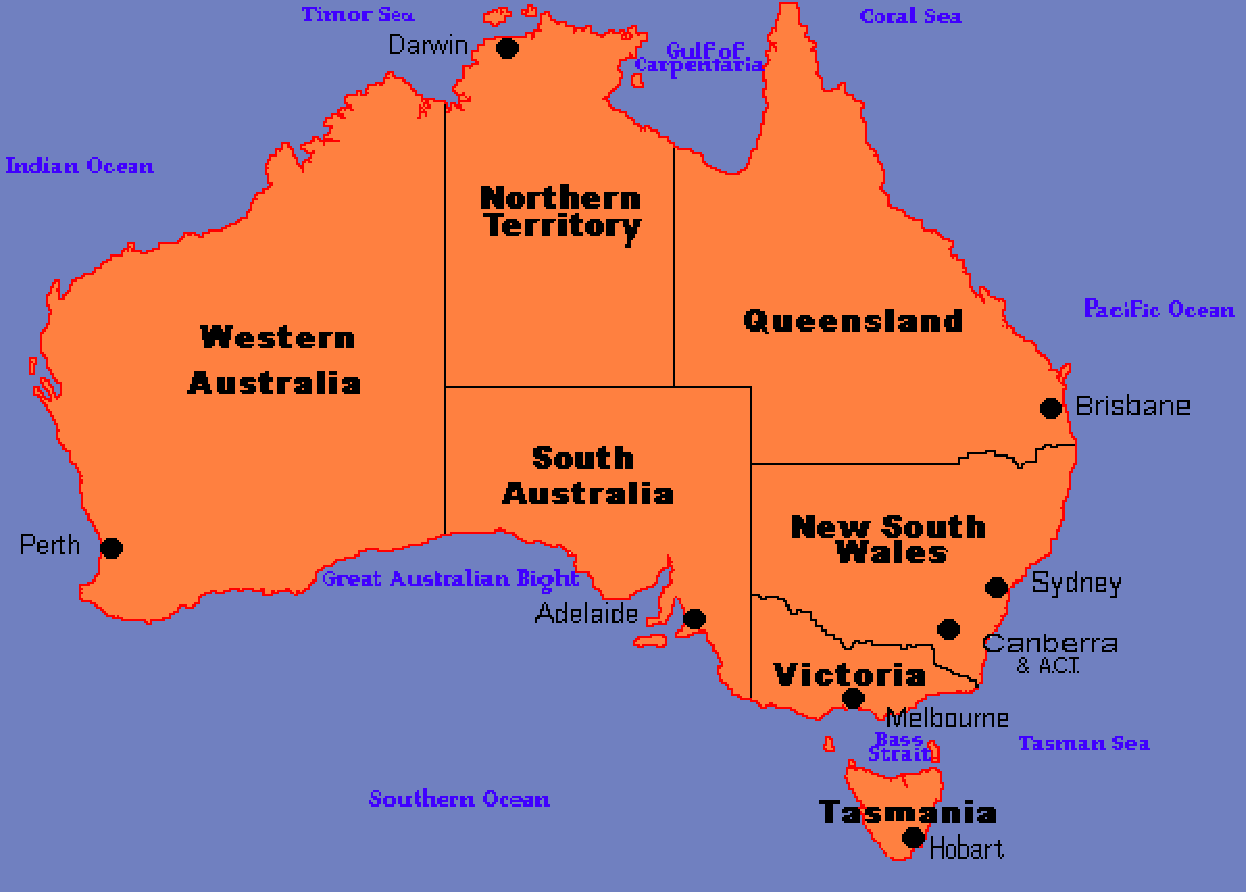
\epsfig{file=Figures/australia.pdf,scale=0.8}} 
  \caption{A map of Australia.}
  \label{fig:australia.pdf}
\end{figure}

\subsection{Example: Map Coloring}
In \href{https://en.wikipedia.org/wiki/Four_color_theorem}{map colouring} a map showing different state
borders is given and the task is to colour the different states such that no two states that have a common
border share the same colour.  \myFig{australia.pdf} shows a map of Australia.  There are seven different
states in Australia:
\begin{enumerate}
\item Western Australia, abbreviated as $\mathrm{WA}$,
\item Northern Territory, abbreviated as $\mathrm{NT}$,
\item South Australia, abbreviated as $\mathrm{SA}$,
\item Queensland, abbreviated as $\mathrm{Q}$,
\item New South Wales, abbreviated as $\mathrm{NSW}$,
\item Victoria, abbreviated as $\mathrm{V}$, and
\item Tasmania, abbreviated as $\mathrm{T}$.
\end{enumerate}
Figure \ref{fig:australia.pdf} would certainly look better if different states had been coloured with different
colours.  For the purpose of 
this example let us assume that we have only three colours available.  The question then is whether it is 
possible to colour the different states in a way that no two neighbouring states share the same colour.  This
problem can be formalized as a constraint satisfaction problem.  To this end we define:
\begin{enumerate}
\item $\mathtt{Vars} := \{ \mathrm{WA}, \mathrm{NT}, \mathrm{SA}, \mathrm{Q}, \mathrm{NSW}, \mathrm{V}, \mathrm{T} \}$,
\item $\mathtt{Values} := \{ \mathtt{red}, \mathtt{green}, \mathtt{blue} \}$,
\item $\mathtt{Constraints} := 
         \bigl\{ \mathrm{WT} \not= \mathrm{NT}, \mathrm{WT} \not= \mathrm{SA},
                 \mathrm{NT} \not= \mathrm{SA}, \mathrm{NT} \not= \mathrm{Q},
                 \mathrm{SA} \not= \mathrm{Q}, \mathrm{SA} \not= \mathrm{NSW}, \mathrm{SA} \not= \mathrm{V}, 
                 \mathrm{V} \not = \mathrm{T}
         \bigr\}
        $
\end{enumerate}
Then $\mathcal{P} := \langle \mathtt{Vars}, \mathtt{Values}, \mathtt{Constraints} \rangle$ is a constraint satisfaction problem.  
If we define the assignment $A$ such that
\begin{enumerate}
\item $A(\mathrm{WA}) = \mathtt{blue}$,
\item $A(\mathrm{NT}) = \mathtt{red}$,
\item $A(\mathrm{SA}) = \mathtt{green}$,
\item $A(\mathrm{Q}) = \mathtt{blue}$,
\item $A(\mathrm{NSW}) = \mathtt{red}$,
\item $A(\mathrm{V}) = \mathtt{blue}$,
\item $A(\mathrm{T}) = \mathtt{red}$,
\end{enumerate}
then you can check that the assignment $A$ is indeed a solution to the constraint satisfaction problem $\mathcal{P}$.

\subsection{Example: The Eight Queens Puzzle}
The \href{https://en.wikipedia.org/wiki/Eight_queens_puzzle}{eight queens problem} asks to put 8 queens onto a
chessboard such that no queen can attack another queen.  In \href{https://en.wikipedia.org/wiki/Chess}{chess},
a queen can attack all pieces that are either in the same row, the same column, or the same diagonal.  If we
want to put 8 queens on a chessboard such that no two queens can attack each other, we have to put exactly one
queen in every row:  If we would put more than one queen in a row, the queens in that row can attack each other.
If we would leave a row empty, then, given that the other rows contain at most one queen, there would be less
than 8 queens on the board.  Therefore, in order to model the eight queens problem as a constraint satisfaction
problem, we will use the following set of variables:
\\[0.2cm]
\hspace*{1.3cm}
$\mathtt{Vars} := \{ \mathtt{V}_1, \mathtt{V}_2, \mathtt{V}_3, \mathtt{V}_4, \mathtt{V}_5, \mathtt{V}_6, \mathtt{V}_7,\mathtt{V}_8 \}$,
\\[0.2cm]
where for $i \in \{1,\cdots,8\}$ the variable $\mathtt{V}i$ specifies the column of the queen that is placed in
row $i$.   As the columns run from one to eight, we define the set $\mathtt{Values}$ as
\\[0.2cm]
\hspace*{1.3cm}
$\mathtt{Values} := \{1,2,3,4,5,6,7,8\}$.
\\[0.2cm]
Next, let us define the constraints.  There are three different types of constraints.
\begin{enumerate}
\item We have constraints that express that no two queens positioned in different rows share the same column.
      To capture these constraints, we define
      \\[0.2cm]
      \hspace*{1.3cm}
      $\mathtt{SameRow} := \bigl\{ \mathtt{V}_i \not= \mathtt{V}_j \bigm| i \in \{1,\cdots,8\} \wedge j \in \{1,\cdots,8\} \wedge j < i \bigr\}$.
      \\[0.2cm]
      Here the condition $i < j$ ensures that, for example, we have the constraint $\mathtt{V}_2 \not= \mathtt{V}_1$
      but not the constraint  $\mathtt{V}_1 \not= \mathtt{V}_2$, as the latter would be redundant if the former is
      already given.
\item We have constraints that express that no two queens positioned in different rows share the same rising
      diagonal.  To capture these constraints, we define
      \\[0.2cm]
      \hspace*{1.3cm}
      $\mathtt{SameRising} := \bigl\{ i + \mathtt{V}_i \not= j + \mathtt{V}_j \bigm| i \in \{1,\cdots,8\} \wedge j \in \{1,\cdots,8\} \wedge j < i \bigr\}$.
\item We have constraints that express that no two queens positioned in different rows share the same falling
      diagonal.  To capture these constraints, we define
      \\[0.2cm]
      \hspace*{1.3cm}
      $\mathtt{SameFalling} := \bigl\{ i - \mathtt{V}_i \not= j - \mathtt{V}_j \bigm| i \in \{1,\cdots,8\} \wedge j \in \{1,\cdots,8\} \wedge j < i \bigr\}$.
\end{enumerate}
Then, the set of constraints is defined as 
\\[0.2cm]
\hspace*{1.3cm}
$\mathtt{Constraints} := \mathtt{SameRow} \cup \mathtt{SameRising} \cup \mathtt{SameFalling}$
\\[0.2cm]
and the eight queens problem can be stated as the constraint satisfaction problem
\\[0.2cm]
\hspace*{1.3cm}
$\mathcal{P} := \langle \mathtt{Vars}, \mathtt{Values}, \mathtt{Constraints} \rangle$.
\\[0.2cm]
If we define the assignment $A$ such that
\\[0.2cm]
\hspace*{1.3cm}
$A(1) := 4,\; A(2) := 8,\; A(3) := 1,\; A(4) := 2,\; A(5) := 6,\; A(6) := 2,\; A(7) := 7,\; A(8) := 5$,
\\[0.2cm]
then it is easy to see that this assignment is a solution of the eight queens problem.  This solution is shown
in \myFig{eight-queens.txt}.


\begin{figure}[!ht]
  \centering
\hspace*{0.0cm}
\vbox{\offinterlineskip
   \hrule height1pt
   \hbox{\vrule width1pt\bigchess
         \vbox{\hbox{0Z0L0Z0Z}
               \hbox{Z0Z0Z0ZQ}
               \hbox{QZ0Z0Z0Z}
               \hbox{Z0L0Z0Z0}
               \hbox{0Z0Z0L0Z}
               \hbox{ZQZ0Z0Z0}
               \hbox{0Z0Z0ZQZ}
               \hbox{Z0Z0L0Z0}}%
         \vrule width1pt}
   \hrule height1pt}

  \caption{A solution of the eight queens problem.}
  \label{fig:eight-queens.txt}
\end{figure}
Later, when we implement procedures to solve  \textsc{Csp}s, we will represent variable assignments and partial
variable assignments as binary relations.  For example, $A$ would then be represented as the relation
\\[0.2cm]
\hspace*{1.3cm}
$A = \bigl\{ \pair(\mathrm{V}_1,4), \pair(\mathrm{V}_2,8), \pair(\mathrm{V}_3,1), \pair(\mathrm{V}_4,2), 
             \pair(\mathrm{V}_5,6), \pair(\mathrm{V}_6,2), \pair(\mathrm{V}_7,7), \pair(\mathrm{V}_8,5) 
     \bigr\}$.
\\[0.2cm]
If we define 
\\[0.2cm]
\hspace*{1.3cm}
$B := \bigl\{ \pair(\mathrm{V}_1,4), \pair(\mathrm{V}_2,8), \pair(\mathrm{V}_3,1) \bigr\}$,
\\[0.2cm]
then $B$ is a partial assignment and $\mathtt{dom}(B) = \{ \mathrm{V}_1, \mathrm{V}_2, \mathrm{V}_3 \}$.  This
partial assignment is shown in \myFig{eight-queens-partial.txt}.

\begin{figure}[!ht]
  \centering
\hspace*{0.0cm}
\vbox{\offinterlineskip
   \hrule height1pt
   \hbox{\vrule width1pt\bigchess
         \vbox{\hbox{0Z0L0Z0Z}
               \hbox{Z0Z0Z0ZQ}
               \hbox{QZ0Z0Z0Z}
               \hbox{Z0Z0Z0Z0}
               \hbox{0Z0Z0Z0Z}
               \hbox{Z0Z0Z0Z0}
               \hbox{0Z0Z0Z0Z}
               \hbox{Z0Z0Z0Z0}}%
         \vrule width1pt}
   \hrule height1pt}

  \caption{The partial assignment $\bigl\{ \pair(\mathrm{V}_1,4), \pair(\mathrm{V}_2,8), \pair(\mathrm{V}_3,1) \bigr\}$.}
  \label{fig:eight-queens-partial.txt}
\end{figure}



\myFig{queens-csp.stlx} shows a \textsc{SetlX} program that can be used to create the eight queens puzzle as a
\textsc{Csp}.  The code shown in this figure is more general than the eight queens puzzle:  Given a natural
number $n$, the function call $\mathtt{queensCSP}(n)$ creates a constraint satisfaction problem $\mathcal{P}$ that generalizes
the eight queens problem to the problem of putting $n$ queens on a board of size $n$ times $n$.

\begin{figure}[!ht]
\centering
\begin{Verbatim}[ frame         = lines, 
                  framesep      = 0.3cm, 
                  firstnumber   = 1,
                  labelposition = bottomline,
                  numbers       = left,
                  numbersep     = -0.2cm,
                  xleftmargin   = 0.8cm,
                  xrightmargin  = 0.8cm,
                ]
    queensCSP := procedure(n) {
        Variables   := { "V$i$" : i in {1..n} };
        Values      := { 1 .. n };
        Constraints := {};
        for (i in [2..n], j in [1..i-1]) {
            Constraints += { "V$i$ != V$j$" };
            Constraints += { "$i$ + V$i$ != $j$ + V$j$" };
            Constraints += { "$i$ - V$i$ != $j$ - V$j$" };
        }
        return [Variables, Values, Constraints];
    };
\end{Verbatim}
\vspace*{-0.3cm}
\caption{\textsc{SetlX} code to create the CSP representing the eight-queens puzzle.}
\label{fig:queens-csp.stlx}
\end{figure}

The beauty of \href{https://en.wikipedia.org/wiki/Constraint_programming}{constraint programming} is the fact
that we will be able to develop a so called \emph{\color{blue}constraint solver} that takes as input a \textsc{Csp}
like the one produced by the program shown in Figure \ref{fig:queens-csp.stlx} and that is then capable of
computing a solution. 

\subsection{Applications}
Besides the toy problems discussed so far, there are a number of industrial applications of constraint
satisfaction problems.  The most important application seem to be variants of
\href{https://en.wikipedia.org/wiki/Scheduling_(production_processes)}{scheduling problems}. 
A simple example of a scheduling problem is the problem of generating a time table for a school.  A school has
various teachers, each of which can teach some subjects but not others.  Furthermore, there are a number of
classes that must be taught in different subjects.  The problem is then to assign teachers to classes and to
create a time table.

\section{Brute Force Search}
The most straightforward algorithm to solve a \textsc{Csp} is to test all possible combinations of assigning
values to variables.  If there are $n$ different values that can be assigned to $k$ variables, this amounts to 
checking $n^k$ different assignments.  For example, for the eight queens problem there are 8 variables and
8 possible values leading to 
\\[0.2cm]
\hspace*{1.3cm}
$8^8 = 16,777,216$
\\[0.2cm]
different assignments that need to be tested.  Given the clock speed of modern computers, checking a million
assignments per second is plausible.  Hence, this approach would be able to solve the eight queens problem in
about 15 minutes.  The approach of testing all possible combinations is known as \emph{\color{blue}brute force search}.
An implementation is shown in \myFig{csp-brute-force.stlx}.

\begin{figure}[!ht]
\centering
\begin{Verbatim}[ frame         = lines, 
                  framesep      = 0.3cm, 
                  firstnumber   = 1,
                  labelposition = bottomline,
                  numbers       = left,
                  numbersep     = -0.2cm,
                  xleftmargin   = 0.8cm,
                  xrightmargin  = 0.8cm,
                ]
    solve := procedure(csp) {
        [Variables, Values, Constraints] := csp;
        return brute_force_search({}, Variables, Values, Constraints);
    };
    brute_force_search := procedure(Assignment, Variables, Values, Constraints) {
        if (Variables == {}) {
            if (check_all_constraints(Assignment, Constraints)) {
                return Assignment;
            }
            return;
        }
        var := from(Variables);
        for (value in Values) {
            NewAss := Assignment + { [var, value] };
            result := brute_force_search(NewAss, Variables, Values, Constraints);
            if (result != om) {
                return result;
            }
        }
    };
\end{Verbatim}
\vspace*{-0.3cm}
\caption{Solving a \textsc{Csp} via brute force search.}
\label{fig:csp-brute-force.stlx}
\end{figure}

The procedure $\mathtt{solve}$ gets a constraint satisfaction problem $\mathtt{cps}$ as its input.  
This $\mathtt{csp}$ is given a triple.  The sole purpose of $\mathtt{search}$ is to extract the components
of this triple and then calls the procedure $\mathtt{brute\_force\_search}$ with the corresponding arguments.

The function $\mathtt{brute\_force\_search}$ takes four arguments.
\begin{enumerate}
\item $\mathtt{Assignment}$ is a partial assignment of values to variables.
      Initially, this assignment will be empty.  Every recursive call of
      $\mathtt{brute\_force\_search}$ adds the assignment of one variable to the given assignment.
\item $\mathtt{Variables}$ is the set of variables of the \textsc{Csp} that is to be solved.
      This set contains only those variables that have not yet been assigned a value.
\item $\mathtt{Values}$ is the set of values of this \textsc{Csp}.
\item $\mathtt{Constraints}$ is the corresponding set of constraints.
\end{enumerate}
The implementation of $\mathtt{brute\_force\_search}$ works as follows:
\begin{enumerate}
\item If all variables have been assigned a value, the set $\mathtt{Variables}$ will be empty.
      Then we test whether all constraints are satisfied.  This is done using the auxiliary
      procedure $\mathtt{check\_all\_constraints}$ that is shown in \myFig{csp-brute-force.stlx-2}.
      If the current $\mathtt{Assignment}$ does indeed satisfy all constraints, it is a solution and
      is returned.

      If, instead, some constraint is not satisfied, then the procedure returns the undefined value $\Omega$.
\item If the assignment is not yet complete, we pick a variable $\mathtt{var}$ from the set of
      $\mathtt{Variables}$ that still have no value assigned.  Then, for every possible
      $\mathtt{value}$ in the set $\mathtt{Values}$, we augment the current partial
      $\mathtt{Assignment}$ to the new assignment
      \\[0.2cm]
      \hspace*{1.3cm}
      \texttt{Assignment + \{ [var, value] \}}.
      \\[0.2cm]
      Then, the algorithm recursively tries to find a solution for this new partial assignment.
      If this recursive call succeeds, the solution is returned.  Otherwise, the next
      $\mathtt{value}$ is tried.
\end{enumerate}


\begin{figure}[!ht]
\centering
\begin{Verbatim}[ frame         = lines, 
                  framesep      = 0.3cm, 
                  firstnumber   = last,
                  labelposition = bottomline,
                  numbers       = left,
                  numbersep     = -0.2cm,
                  xleftmargin   = 0.8cm,
                  xrightmargin  = 0.8cm,
                ]
    check_all_constraints := procedure(Assignment, Constraints) {
        for (f in Constraints) {
            Vars := collectVars(f);
            if (!eval_constraint(Assignment, f, Vars)) {
                return false;
            }
        }
        return true;
    };       
    eval_constraint := procedure(Assignment, Formula, Vars) {
        for (v in Vars) {
            execute("$v$ := $Assignment[v]$;");
        }
        return eval(Formula);
    };
\end{Verbatim}
\vspace*{-0.3cm}
\caption{Auxiliary procedures for brute force search.}
\label{fig:csp-brute-force.stlx-2}
\end{figure}

The function $\mathtt{check\_all\_constraints}$ takes a complete variable $\mathtt{Assignment}$ as
its first input.  The second input is the set of $\mathtt{Constraints}$.  For all constraints
$\mathtt{f}$, it computes the set of variables $\mathtt{Vars}$ occurring in $\mathtt{f}$.  Then the
constraint $\mathtt{f}$ is evaluated.  If the evaluation of any of the constraints returns
$\mathtt{false}$, the function returns $\mathtt{false}$.  Otherwise, $\mathtt{true}$ is returned.

The procedure $\mathtt{eval\_constraint}$ takes a partial $\mathtt{Assignment}$, a $\mathtt{Formula}$
that is supposed to be a constraint, and the set of variables $\mathtt{Vars}$ that occur in
$\mathtt{Formula}$.  Its purpose is to evaluate $\mathtt{Formula}$ using the $\mathtt{Assignment}$.  In
order for this to be possible we have to assume that
\\[0.2cm]
\hspace*{1.3cm}
$\mathtt{var}(\mathtt{Formula)} \subseteq \mathtt{dom}(\mathtt{Assignment})$,
\\[0.2cm]
i.e.~all variables occurring in $\mathtt{Formula}$ have a value assigned in $\mathtt{Assignment}$.

The $\mathtt{Formula}$ is evaluated by first assigning the value prescribed in $\mathtt{Assignment}$ to
all variables $\mathtt{v}$ occurring in $\mathtt{Vars}$.  Once these assignments have been executed in
the \texttt{for}-loop, the $\mathtt{Formula}$ can be evaluated using the procedure $\mathtt{eval}$, which
is one of the predefined procedures in \textsc{SetlX}.

When I tested this brute force search with the eight queens problem, it took about 510 seconds to
compute a solution.  In contrast, the seven queens problem only took 45 seconds.  As we have
\\[0.2cm]
\hspace*{1.3cm}
$\ds\frac{8^8}{7^7} \approx 20.3$ \quad \and \quad $\ds\frac{510}{45} \approx 11.3$
\\[0.2cm]
this shows that the computation time does indeed grow with the number of possible assignments that
have to be checked.  However, the correspondence is not exact.  The reason is that we stop our
search as soon as a solution is found.  If we are lucky and the given \textsc{Csp} is easy to solve, this
might happen when we have checked only a small portion of the space of possible assignments.

\section{Backtracking Search}
One simple approach to solve a \textsc{Csp} is via \emph{\color{blue}backtracking}.
\myFig{csp-backtrack-solver.stlx-1} shows a simple \textsc{Csp} solver that employs backtracking.  We discuss
this program next.

\begin{figure}[!ht]
\centering
\begin{Verbatim}[ frame         = lines, 
                  framesep      = 0.3cm, 
                  firstnumber   = 1,
                  labelposition = bottomline,
                  numbers       = left,
                  numbersep     = -0.2cm,
                  xleftmargin   = 0.8cm,
                  xrightmargin  = 0.8cm,
                ]
    solve := procedure(csp) {
        [Vars, Vals, Constrs] := csp;
        csp := [Vars, Vals, { [f, collectVars(f)] : f in Constrs }];
        check {
            return bt_search({}, csp);
        }
    };
    bt_search := procedure(Assignment, csp) {
        [Variables, Values, Constraints] := csp;
        if (#Assignment == #Variables) {
            return Assignment;
        }
        var := select_unassigned_variable(Assignment, Variables);
        for (value in Values) {
            check {
                if (is_consistent(var, value, Assignment, Constraints)) {
                    return bt_search(Assignment + { [var, value] }, csp);
                }
            }
        }
        backtrack;
    };
\end{Verbatim}
\vspace*{-0.3cm}
\caption{A backtracking \textsc{Csp} solver.}
\label{fig:csp-backtrack-solver.stlx-1}
\end{figure}
The procedure $\mathtt{solve}$ takes a constraint satisfaction problem $\mathtt{csp}$ as input and tries to
find a solution.  
\begin{enumerate}
\item First, the $\mathtt{csp}$ is split into its components.
\item Next, for every constraint $\mathtt{f}$ of the given $\mathtt{csp}$, we compute the set of variables that
      are used in $\mathtt{f}$.  These variables are then stored together with the constraint $\mathtt{f}$ and
      the correspondingly modified data structure is stored in $\mathtt{csp}$ and is called an
      \emph{\color{blue}augmented \textsc{Csp}}.

      The reason to compute and store these variables is efficiency: When we later check whether a constraint $\mathtt{f}$
      is satisfied for a partial variable assignment $B$, we only need to check the constraint $\mathtt{f}$ iff all
      of its variables are members of the domain of $B$.
\item Next, we call the procedure $\mathtt{bt\_search}$ to compute a solution of $\mathtt{csp}$.
      This procedure is enclosed in a \texttt{check}-block.  Conceptually, this \texttt{check}-block is the
      same as if we had enclosed the call to $\mathtt{bt\_search}$ in a \texttt{try}-\texttt{catch}-block as
      shown below:
\begin{verbatim}
      try {
          return bt_search({}, csp);
      } catch(e) {}
\end{verbatim}
     The point is that the procedure $\mathtt{bt\_search}$ either returns a solution or, if it is not able to
     find a solution, it throws a special kind of exception, a so called \emph{\color{blue}backtrack exception}.
     The \texttt{check}-block ensures that this exception is silently discarded.  It is just a syntactical
     convenience that is more concise than using \texttt{try} and \texttt{catch}.
\end{enumerate}
Next, we discuss the procedure $\mathtt{bt\_search}$.  This procedure gets a partial assignment
$\mathtt{Assignment}$ as input together with an augmented $\mathtt{csp}$.  This partial assignment is
\emph{\color{blue}consistent} with $\mathtt{csp}$:  If $\mathtt{f}$ is a constraint of $\mathtt{csp}$ such that
all the variables occurring in $\mathtt{f}$ are members of $\mathtt{dom}(\mathtt{Assignment})$, then evaluating
$\mathtt{f}$ using $\mathtt{Assignment}$ yields $\mathtt{true}$.  Initially, this partial assignment is empty
and hence trivially consistent.  The idea is to extend this partial assignment until it is a complete
assignment that satisfies all constraints of the given $\mathtt{csp}$.
\begin{enumerate}
\item First, the augmented $\mathtt{csp}$ is split into its components.
\item Next, if $\mathtt{Assignment}$ is already a complete variable assignment, it is a solution of
      $\mathtt{csp}$ and this solution is returned.  Since $\mathtt{Assignment}$ is represented as a binary
      relation, $\mathtt{Assignment}$ is complete if its size is the same as the size of $\mathtt{Variables}$.
\item Otherwise, we have to extend the partial $\mathtt{Assignment}$.  In order to do so, we first have to
      select a variable $\mathtt{var}$ that has not yet been assigned a value.  This is done using the
      auxiliary procedure $\mathtt{select\_unassigned\_variable}$ that is shown in
      \myFig{csp-backtrack-solver.stlx-2} and will be discussed later.
\item Next, it is tried to assign a $\mathtt{value}$ to the selected variable $\mathtt{var}$.  It is checked
      whether this assignment would be consistent using the procedure $\mathtt{is\_consistent}$.
      If the partial assignment turns out to be consistent, the partial $\mathtt{assignment}$
      is extended to the new partial assignment
      \\[0.2cm]
      \hspace*{1.3cm}
      \texttt{Assignment + \{ [var, value] \}}.
      \\[0.2cm]
      Then, the procedure $\mathtt{bt\_search}$ is called recursively to complete this new partial assignment.
      If this is successful, the resulting assignment is a solution that is returned.  Otherwise,
      the recursive call of $\mathtt{bt\_search}$ will instead raise an exception.  This exception is muted 
      by the \texttt{check}-block that surrounds the call to $\mathtt{bt\_search}$.  In that case, the
      \texttt{for}-loop generates a new possible $\mathtt{value}$ that can be assigned to the variable
      $\mathtt{var}$.  If all possible values have been tried and none was successful, the \texttt{for}-loop
      ends and the \texttt{backtrack}-statement is executed.  Effectively, this statement raises an exception
      that is caught by one of \texttt{check}-blocks.
\end{enumerate}


\begin{figure}[!ht]
\centering
\begin{Verbatim}[ frame         = lines, 
                  framesep      = 0.3cm, 
                  firstnumber   = 1,
                  labelposition = bottomline,
                  numbers       = left,
                  numbersep     = -0.2cm,
                  xleftmargin   = 0.8cm,
                  xrightmargin  = 0.8cm,
                ]
    select_unassigned_variable := procedure(Assignment, Variables) {
        return rnd({ v : v in Variables | Assignment[v] == om });
    };
    is_consistent := procedure(var, value, Assignment, Constraints) {
       NewAssignment := Assignment + { [var, value] };
       for ([Formula, Vars] in Constraints | var in Vars) {
             if (Vars <= domain(NewAssignment)) {
                if (!eval_constraint(NewAssignment, Formula, Vars)) {
                    return false;
                }
            }
        }
        return true;
    };
\end{Verbatim}
\vspace*{-0.3cm}
\caption{Auxiliary procedures for the \textsc{Csp} solver shown in Figure \ref{fig:csp-backtrack-solver.stlx-1}}
\label{fig:csp-backtrack-solver.stlx-2}
\end{figure}

We still need to discuss the implementation of the auxiliary procedures shown in \myFig{csp-backtrack-solver.stlx-2}. 
\begin{enumerate}
\item The procedure $\mathtt{select\_unassigned\_variable}$ takes a partial $\mathtt{Assignment}$ and the set
      of all $\mathtt{Variables}$.  It randomly selects a variable $\mathtt{v}$ such that 
      \\[0.2cm]
      \hspace*{1.3cm}
      $\mathtt{v} \not\in \mathtt{dom}(\mathtt{Assignment})$
      \\[0.2cm]
      which is the case if $\mathtt{Assignment}[v] = \Omega$.

      It is certainly possible to be more clever here.  We will later show that it is beneficial to select a
      variable that is a \emph{\color{blue}most constrained variable}, i.e.~a variable such that the number of
      values that can be assigned to this variable while still having a consistent assignment is minimal.
\item The procedure $\mathtt{is\_consistent}$ takes a variable $\mathtt{var}$, a $\mathtt{value}$, a partial 
      $\mathtt{Assignment}$ and a set of $\mathtt{Constraints}$.  It is assumed that $\mathtt{Assignment}$ is
      \emph{\color{blue}partially consistent} with respect to the set $\mathtt{Constraints}$, i.e.~for every formula $\mathtt{f}$
      occurring in $\mathtt{Constraints}$ such that $\mathtt{vars}(\mathtt{f}) \subseteq \mathtt{dom}(\mathtt{Assignment})$
      the formula $\mathtt{f}$ evaluates to $\mathtt{true}$ using $\mathtt{Assignment}$.  The purpose of
      $\mathtt{is\_consistent}$ is to check, whether the extended assignment
      \\[0.2cm]
      \hspace*{1.3cm}
      $\mathtt{NewAssignment} \;\mathtt{:=}\;\mathtt{Assignment} \cup \{ \pair(\mathtt{var}, \mathtt{value}) \}$
      \\[0.2cm]
      that assigns $\mathtt{value}$ to the variable $\mathtt{var}$ is still partially consistent with $\mathtt{Constraints}$. 
      To this end, the \texttt{for}-loop iterates over all $\mathtt{Formula}$ in $\mathtt{Constraints}$. 
      However, we only have to check those $\mathtt{Formula}$ that contain the variable $\mathtt{var}$ and,
      furthermore, have all their variables occurring in $\mathtt{dom}(\mathtt{NewAssignment})$.  The reasoning
      is as follows:
      \begin{enumerate}
      \item If $\mathtt{var}$ does not occur in $\mathtt{Formula}$, then adding $\mathtt{var}$ to
            $\mathtt{Assignment}$ cannot change the result of evaluating $\mathtt{Formula}$ and as
            $\mathtt{Assignment}$ is assumed to be partially consistent with respect to $\mathtt{Formula}$, 
            $\mathtt{NewAssignment}$ is also partially consistent with respect to $\mathtt{Formula}$.
      \item If $\mathtt{dom}(\mathtt{NewAssignment}) \not\subseteq \mathtt{Vars}$, then $\mathtt{Formula}$ can not be evaluated anyway.
      \end{enumerate}
      Now if any of the $\mathtt{Formula}$ evaluates to $\mathtt{false}$, then $\mathtt{NewAssignment}$ is not
      partially consistent and we can immediately return $\mathtt{false}$.  Otherwise, $\mathtt{true}$ is returned.
\end{enumerate}  

\section{Constraint Propagation}
Once we choose a value for a variable, this choice influences the values that are still available for other variables.
For example, suppose we place the queen in row 1 in the second column, then no other queen can be placed in
that column.   Additionally, the queen in row 2 can then not be placed in any of the first three columns.
It turns out that elaborating this idea can enhance the performance of backtracking search considerably.
\myFig{csp-constraint-propagation.stlx-1} shows an implementation of \emph{\color{blue}constraint propagation}.
This implementation is also able to handle \emph{\color{blue}unary constraints}, i.e.~constraints that contain
only a single variable.

\begin{figure}[!ht]
\centering
\begin{Verbatim}[ frame         = lines, 
                  framesep      = 0.3cm, 
                  firstnumber   = 1,
                  labelposition = bottomline,
                  numbers       = left,
                  numbersep     = -0.2cm,
                  xleftmargin   = 0.8cm,
                  xrightmargin  = 0.8cm,
                ]
    solve := procedure(csp) {
        [Variables, Values, Constrs] := csp;
        ValuesPerVar  := { [v, Values] : v in Variables };
        Annotated     := { [f, collectVars(f)] : f in Constrs };
        UnaryConstrs  := { [f, V] : [f, V] in Annotated | #V == 1 };
        BinaryConstrs := { [f, V] : [f, V] in Annotated | #V == 2 };
        msg := "Constraints should be either unary or binary!";
        assert(UnaryConstrs + BinaryConstrs == Annotated, msg); 
        for ([f, V] in UnaryConstrs) {
            var               := arb(V);
            ValuesPerVar[var] := solve_unary(f, var, ValuesPerVar[var]);
        }
        check {
            return bt_search({}, [Variables, ValuesPerVar, BinaryConstrs]);
        }
    };
\end{Verbatim}
\vspace*{-0.3cm}
\caption{Constraint Propagation.}
\label{fig:csp-constraint-propagation.stlx-1}
\end{figure}

In order to implement constraint propagation, it is necessary to administer the values that can be used
to instantiate the different variables separately, i.e.~for every variable $\mathtt{v}$ we need to know which
values are admissible for $\mathtt{v}$.  To this end, we need a dictionary that contains the set of possible
values for every variable $\mathtt{v}$.  Initially, this dictionary assigns the set $\mathtt{Values}$ to
every variable.  Next, we take care of the unary constraints and shrink these sets accordingly.  Then we solve
the binary constraints and shrink these sets even more once we assign values to variables.
\begin{enumerate}
\item The procedure $\mathtt{solve}$ receives a $\mathtt{csp}$.  This $\mathtt{csp}$ is first split into its three components.
\item The first task of $\mathtt{solve}$ is to create the dictionary $\mathtt{ValuesPerVar}$.  
      Given a variable $\mathtt{v}$, this dictionary assigns the set of values that can be used to instantiate this
      variable.  Initially, this set is the same for all variables and is equal to $\mathtt{Values}$.
\item Next, for every constraint $\mathtt{f}$, the dictionary $\mathtt{Annotated}$ attaches the
      variables occurring in a constraint $\mathtt{f}$ to $\mathtt{f}$.
\item In order to solve the unary constraints we first have to find them.
      The set $\mathtt{UnaryConstrs}$ contains all those pairs $[\mathtt{f}, \mathtt{V}]$ from the set of
      annotated constraints $\mathtt{Annotated}$ such that the set of variables $\mathtt{V}$ contains just a
      single variable. 
\item Similarly, the set $\mathtt{BinaryConstrs}$ contains those constraints that involve two variables.
\item We assume that the set of constraints $\mathtt{Annotated}$ only contains unary and binary constraints.
\item In order to solve the unary constraints, we iterate over all unary constraints and shrink the set of
      values associated with the variable occurring in the constraint accordingly.
\item Then, the dictionaries $\mathtt{VariablesPerVar}$ and $\mathtt{BinaryConstrs}$ are combined with the set
      of $\mathtt{Variables}$ into a triple that is used as the argument to the call of $\mathtt{bt\_search}$.
\end{enumerate}

\begin{figure}[!ht]
\centering
\begin{Verbatim}[ frame         = lines, 
                  framesep      = 0.3cm, 
                  firstnumber   = 1,
                  labelposition = bottomline,
                  numbers       = left,
                  numbersep     = -0.2cm,
                  xleftmargin   = 0.8cm,
                  xrightmargin  = 0.8cm,
                ]
    solve_unary := procedure(constraint, variable, Values) {
        LegalValues := {};
        for (value in Values) {
            Assignment := { [variable, value] };
            if (eval_constraint(Assignment, constraint, { variable })) {
                LegalValues += { value };
            }
        }
        return LegalValues;
    };
\end{Verbatim}
\vspace*{-0.3cm}
\caption{Implementation of $\mathtt{solve\_unary}$.}
\label{fig:csp-constraint-propagation.stlx:solve_unary}
\end{figure}

The function $\mathtt{solve\_unary}$ shown in \myFig{csp-constraint-propagation.stlx:solve_unary} takes a unary
$\mathtt{constraint}$, a $\mathtt{variable}$ and the set of $\mathtt{Values}$ that can be assigned to this
$\mathtt{variable}$.  It returns the subset of values that satisfy the given $\mathtt{constraint}$.
\begin{enumerate}
\item To achieve its goal, $\mathtt{solve\_unary}$ iterates over all possible $\mathtt{Values}$.  
\item Next, for every $\mathtt{value}$ in the set $\mathtt{Values}$, an $\mathtt{Assignment}$ is created that assign
      the $\mathtt{value}$ to this $\mathtt{variable}$.
\item Then the $\mathtt{constraint}$ is evaluated with this $\mathtt{Assignment}$.
\item If the $\mathtt{constraint}$ is satisfied under this $\mathtt{Assignment}$, the $\mathtt{value}$ is added to the set
      $\mathtt{LegalValues}$, which is the set of values which satisfy the unary $\mathtt{constraint}$.
\item Finally, the set of $\mathtt{LegalValues}$ is returned.
\end{enumerate}

\begin{figure}[!ht]
\centering
\begin{Verbatim}[ frame         = lines, 
                  framesep      = 0.3cm, 
                  firstnumber   = 1,
                  labelposition = bottomline,
                  numbers       = left,
                  numbersep     = -0.2cm,
                  xleftmargin   = 0.8cm,
                  xrightmargin  = 0.8cm,
                ]
    bt_search := procedure(Assignment, csp) {
        [Variables, Values, Constraints] := csp;
        if (#Assignment == #Variables) {
            return Assignment;
        }
        x := most_constrained_variable(Assignment, Values);
        for (val in Values[x]) {
            check {
                if (is_consistent(x, val, Assignment, Constraints)) {
                    NewVals := propagate(x, val, Assignment, Constraints, Values);
                    csp     := [Variables, NewVals, Constraints];
                    return bt_search(Assignment + { [x, val] }, csp);
                }
            }
        }
        backtrack;
    };
\end{Verbatim}
\vspace*{-0.3cm}
\caption{Implementation of $\mathtt{bt\_search}$.}
\label{fig:csp-constraint-propagation.stlx:bt_search}
\end{figure}

The procedure $\mathtt{bt\_search}$ shown in \myFig{csp-constraint-propagation.stlx:bt_search} is called with a
partial $\mathtt{Assignment}$ that is guaranteed to be 
consistent and a $\mathtt{csp}$.  It tries to complete $\mathtt{Assignment}$ and thereby computes a solution to the $\mathtt{csp}$.
\begin{enumerate}
\item First, it decomposes the $\mathtt{csp}$ into its components:
      \begin{enumerate}
      \item $\mathtt{Values}$ is a dictionary assigning to every variable $\mathtt{v}$ the set of values 
            that can be used to instantiate $\mathtt{v}$.  On recursive invocations of $\mathtt{bt\_search}$
            these sets will shrink.
      \item $\mathtt{Constraints}$ is a dictionary that assigns to every constraint $\mathtt{f}$ the set of
            variables occurring in $\mathtt{f}$.
      \end{enumerate}
\item If the partial $\mathtt{Assignment}$ is already complete, i.e.~if it assigns a value to every variable, 
      then a solution to the given $\mathtt{csp}$ has been found and this solution is returned.
\item Otherwise, we choose a variable $\mathtt{x}$ such that the number of values that can still be used to
      instantiate $\mathtt{x}$ is minimal.  This variable is computed using the procedure
      $\mathtt{most\_constrained\_variable}$ that is shown in \myFig{csp-constraint-propagation.stlx-2}.
\item Next, all values that are still available for $\mathtt{x}$ are tried.  Note that since
      $\mathtt{Values[x]}$ is, in general, smaller than the set of all values of the $\mathtt{csp}$,
      the \texttt{for}-loop in this version of backtracking search is more efficient than the version discussed
      in the previous section. 
\item If is is consistent to assign $\mathtt{val}$ to the variable $\mathtt{x}$, we propagate the consequences
      of this assignment using the procedure $\mathtt{propagate}$ shown in
      \myFig{csp-constraint-propagation.stlx-2}.
      This procedure updates the values that are still allowed for the variables of the $\mathtt{csp}$ once the
      value $\mathtt{val}$ has been assigned to the variable $\mathtt{x}$.
\item Finally, the partial variable $\mathtt{Assignment}$ is updated to include the assignment of 
      $\mathtt{val}$ to $\mathtt{x}$ and the recursive call to $\mathtt{bt\_search}$ tries to complete this new
      assignment. 
\end{enumerate}

\begin{figure}[!ht]
\centering
\begin{Verbatim}[ frame         = lines, 
                  framesep      = 0.3cm, 
                  firstnumber   = 1,
                  labelposition = bottomline,
                  numbers       = left,
                  numbersep     = -0.2cm,
                  xleftmargin   = 0.8cm,
                  xrightmargin  = 0.8cm,
                ]
    most_constrained_variable := procedure(Assignment, Values) {
        Unassigned := { [x, U] : [x, U] in Values | Assignment[x] == om };
        minSize    := min({ #U : [x, U] in Unassigned });
        return rnd({ x : [x, U] in Unassigned | #U == minSize });
    };
    propagate := procedure(x, v, Assignment, Constraints, Values) {
        NewAssignment := Assignment + { [x, v] };
        Values[x]     := { v };
        for ([Formula, Vars] in Constraints | x in Vars) {
            y := arb(Vars - { x });  // Assume binary constraints!!!
            if (!(y in domain(NewAssignment))) {
                NewValues := Values[y];
                for (w in Values[y]) {
                    A2 := NewAssignment + { [y, w] };
                    if (!eval_constraint(A2, Formula, Vars)) {
                        NewValues -= { w };
                    }
                }
                if (NewValues == {}) { backtrack; }
                Values[y] := NewValues;
            }
        }
        return Values;
    };
\end{Verbatim}
\vspace*{-0.3cm}
\caption{Constraint Propagation.}
\label{fig:csp-constraint-propagation.stlx-2}
\end{figure}
\myFig{csp-constraint-propagation.stlx-2} show the implementation of the procedures $\mathtt{most\_constrained\_variable}$
and $\mathtt{propagate}$.  The procedure $\mathtt{most\_constrained\_variable}$ takes a partial
$\mathtt{Assignment}$ and a dictionary $\mathtt{Values}$ returning the set of allowed values for all variables as input.
\begin{enumerate}
\item First, this procedure computes the set of $\mathtt{Unassigned}$ variables.  For every variable $\mathtt{x}$ that
      has not yet been assigned a value in $\mathtt{Assignment}$ this set contains the pair 
      $[\mathtt{x}, \mathtt{U}]$, where $\mathtt{U}$ is the set of allowable values for the variable  $\mathtt{x}$.
\item Next, it computes from all unassigned variables $\mathtt{x}$ the number of values $\mathtt{\#U}$ 
      that can be assigned to $\mathtt{x}$.  From these numbers, the minimum is computed and stored in $\mathtt{minSize}$.  
\item Finally, the set of variables that are maximally constrained is computed.  These are all those variables
      $\mathtt{x}$ such that $\mathtt{Values[x]}$ has size $\mathtt{minSize}$.  From these variables, a random
      variable is returned.
\end{enumerate}
The function $\mathtt{propagate}$ takes the following inputs:
\begin{enumerate}[(a)]
\item $\mathtt{x}$ is a variable.
\item $\mathtt{v}$ is a value that is assigned to the variable $\mathtt{x}$.
\item $\mathtt{Assignment}$ is a partial assignment that contains only assignments for variables that are
      different from $\mathtt{x}$.
\item $\mathtt{Constraints}$ is a set of annotated constraints, i.e.~this set contains pairs of the form 
      $\mathtt{[Formula, Vars]}$, where $\mathtt{Formula}$ is a constraint and $\mathtt{Vars}$ is the set of
      variables occurring in $\mathtt{Formula}$.
\item $\mathtt{Values}$ is a dictionary assigning sets of values to the different variables.
\end{enumerate}
The function $\mathtt{propagate}$ updates the dictionary $\mathtt{Values}$ by taking into account the
consequences of assigning the value $\mathtt{v}$ to the variable $\mathtt{x}$.
\begin{enumerate}
\item The partial $\mathtt{Assignment}$ is updated to $\mathtt{NewAssignment}$, where $\mathtt{NewAssignment}$
      maps $\mathtt{x}$ to $\mathtt{v}$.
\item As $\mathtt{x}$ now has the value of $\mathtt{v}$, the corresponding entry in the dictionary
      $\mathtt{Values}$ is changed accordingly. 
\item Next, $\mathtt{propagate}$ iterates over all $\mathtt{Constraints}$ such that $\mathtt{x}$ occurs in 
      $\mathtt{Formula}$.
\item The implementation of $\mathtt{propagate}$ shown in \myFig{csp-constraint-propagation.stlx-2} assumes
      that all constraints are \emph{\color{blue}binary constraints}, i.e.~if $\mathtt{Formula}$ is a
      constraint, then $\mathtt{Formula}$ contains exactly two different variables.
      As one of these variables is $\mathtt{x}$, the other variable is called $\mathtt{y}$.
\item If the variable $\mathtt{y}$ has already been assigned a value, then there is nothing to do because
      we already know that the assignment $\mathtt{NewAssignment}$ is consistent.  This is ensured by the
      previous call to the function $\mathtt{is\_consistent}$ in the body of the procedure $\mathtt{bt\_search}$.

      However, if $\mathtt{y}$ is still unassigned, it is necessary to update $\mathtt{Values}[y]$.
\item To this end, all values $\mathtt{w}$ in $\mathtt{Values[y]}$ are tested.  
      If it turns out that assigning the value $\mathtt{w}$ to the variable $\mathtt{y}$ violates the
      constraint $\mathtt{Formula}$, then $\mathtt{Values[y]}$ must not contain the value $\mathtt{w}$ 
      and, accordingly, this value is removed from $\mathtt{Values[y]}$.
\item If it turns out that $\mathtt{Values[y]}$ has been reduced to the empty set, then this means that the
      partial assignment $\mathtt{NewAssignment}$ can not be completed.  Hence, the search has to
      $\mathtt{backtrack}$.
\end{enumerate}
I have tested the program described in this section using the $n$ queens puzzle. 
I have found that the time needed to solve ten
instances of 16 queens problem went down from 72 seconds to just 5 seconds.  The procedure is even able to
solve the 32 queens problem, taking about 4 seconds on average, while the version of backtracking search that
does not use constraint propagation took more than 3 minutes on average.


\exercise
There are many different versions of the \href{https://en.wikipedia.org/wiki/Zebra_Puzzle}{\emph{zebra puzzle}}.  
The version below is taken from \href{https://en.wikipedia.org/wiki/Zebra_Puzzle}{\emph{Wikipedia}}.  The
puzzle reads as follows:
\begin{enumerate}
\item There are five houses.
\item The Englishman lives in the red house.
\item The Spaniard owns the dog.
\item Coffee is drunk in the green house.
\item The Ukrainian drinks tea.
\item The green house is immediately to the right of the ivory house.
\item The Old Gold smoker owns snails.
\item Kools are smoked in the yellow house.
\item Milk is drunk in the middle house.
\item The Norwegian lives in the first house.
\item The man who smokes Chesterfields lives in the house next to the man with the fox.
\item Kools are smoked in the house next to the house where the horse is kept.
\item The Lucky Strike smoker drinks orange juice.
\item The Japanese smokes Parliaments.
\item The Norwegian lives next to the blue house.
\item Who drinks water? 
\item Who owns the zebra?
\end{enumerate}
In order to solve the puzzle, we also have to know the following facts:
\begin{enumerate}
\item Each of the five houses is painted in a {\color{blue}different} color.
\item The inhabitants of the five houses are of {\color{blue}different} nationalities,
\item they own {\color{blue}different} pets, 
\item they drink {\color{blue}different} beverages, and 
\item they smoke {\color{blue}different} brands of cigarettes. 
\end{enumerate}
Formulate the zebra puzzle as a constraint satisfaction problem and solve the puzzle using the program
discussed in this section.  You should also try to solve the puzzle using the program given in the previous
section.  Compare the results.
\eoxs


\section{Local Search}
There is another approach to solve constraint satisfaction problems.  This approach is known as
\emph{\color{blue}local search}.  The basic idea is simple: Given as constraint satisfaction problem 
$\mathcal{C}$ of the form 
\\[0.2cm]
\hspace*{1.3cm}
$\mathcal{C} := \langle V, C, D \rangle$,
\\[0.2cm] 
local search works as follows:
\begin{enumerate}
\item Initialize the values of the variables in $V$ randomly.  
\item If all constraints are satisfied, return the solution.
\item For every variable $x \in V$, count the number of \underline{unsatisfied} constraints that involve the
      variable $x$. 
\item Set $\mathtt{maxNum}$ to be the biggest number of unsatisfied constraints for a single variable.
\item Compute the set $\mathtt{maxVars}$ of those variables that have $\mathtt{maxNum}$ unsatisfied constraints.
\item Randomly choose a variable $x$ from the set $\mathtt{maxVars}$.
\item Find a value $d \in D$ such that by assigning $d$ to the variable $x$, the number of unsatisfied constraints is
      minimized.  

      If there is more than one value $d$ with this property, choose the value $d$ randomly from those values
      that minimize the number of unsatisfied constraints.
\item Goto step 2 and repeat until a solution is found.
\end{enumerate}

\begin{figure}[!ht]
\centering
\begin{Verbatim}[ frame         = lines, 
                  framesep      = 0.3cm, 
                  firstnumber   = 1,
                  labelposition = bottomline,
                  numbers       = left,
                  numbersep     = -0.2cm,
                  xleftmargin   = 0.8cm,
                  xrightmargin  = 0.8cm,
                ]
    solve := procedure(n) {
        Queens := [];
        for (row in [1 .. n]) {
            Queens[row] := rnd({1 .. n});
        }
        iteration := 0;
        while (true) {
            Conflicts   := { [numConflicts(Queens, row), row] : row in [1 ..n] };
            [maxNum, _] := last(Conflicts);
            if (maxNum == 0) {
                return Queens;
            }
            if (iteration % 10 != 0) { // avoid infinite loops
                row := rnd({ row : [num, row] in Conflicts | num == maxNum });
            } else {
                row := rnd({ 1 .. n });
            }
            Conflicts := {};
            for (col in [1 .. n]) {
                Board      := Queens;
                Board[row] := col;
                Conflicts  += { [numConflicts(Board, row), col] };
            }
            [minNum, _] := first(Conflicts);
            Queens[row] := rnd({ col : [num, col] in Conflicts | num == minNum });
            iteration   += 1;
        }
    };
\end{Verbatim}
\vspace*{-0.3cm}
\caption{Solving the $n$ queens problem using local search.}
\label{fig:constraints.stlx}
\end{figure}

\noindent
\myFig{constraints.stlx} shows an implementation of these ideas in \textsc{SetlX}.  Instead of solving an
arbitrary constraint satisfaction problem, the program solves the $n$ queens problem.  We proceed to discuss
this program line by line.
\begin{enumerate}
\item The procedure $\mathtt{solve}$ takes one parameter $\mathtt{n}$, which is the size of the chess board.  If
      the computation is successful, $\mathtt{solve(n)}$ returns a list of length $\mathtt{n}$.  Lets call this
      list $\mathtt{Queens}$. For every row $\mathtt{r} \in \{1, \cdots, \mathtt{n}\}$, the value $\mathtt{Queens[r]}$ specifies that the queen 
      that resides in row $\mathtt{r}$ is positioned in column $\mathtt{Queens[r]}$.
\item The \texttt{for} loop initializes the positions of the queens to random values from the set
      $\{1, \cdots, \mathtt{n}\}$.  Effectively, for every row on the chess board, this puts a queen in a
      random column.
\item The variable $\mathtt{iteration}$ counts the number of times that we need to reassign a queen in a given row.
\item All the remaining statements are surrounded by a \texttt{while} loop that is only terminated once a
      solution has been found.
\item The variable $\mathtt{Conflicts}$ is a set of pairs of the form $[c, r]$, where $c$ is the number of
      times the queen in row $r$ is attacked by other queens.  Hence, $c$ is the same as the number of
      unsatisfied conflicts for the variable specifying the column of the queen in row $r$.
\item $\mathtt{maxNum}$ is the maximum of the number of conflicts for any row.
\item If this number is $0$, then all constraints are satisfied and the list $\mathtt{Queens}$ is a solution to the
      $\mathtt{n}$ queens problem.
\item Otherwise, we compute those rows that exhibit the maximal number of conflicts.  From these rows
      we select one $\mathtt{row}$ arbitrarily.
\item The reason for enclosing the assignment to $\mathtt{row}$ in an \texttt{if} statement is explained later. 
      On a first reading of  this program,  this \texttt{if} statement should be ignored.
\item Now that we have identified the $\mathtt{row}$ where the number of conflicts is biggest, we need to
      reassign $\mathtt{Queens[row]}$.  Of course, when reassigning this variable, we would like to have fewer
      conflicts after the reassignment.  Hence, we test all columns to find the best column that can be
      assigned for the queen in the given $\mathtt{row}$.  This is done in a \texttt{for} loop that runs over
      all possible columns.  The set $\mathtt{Conflicts}$ that is maintained in this loop is a set of pairs
      of the form $[k, c]$ where $k$ is the number of times the queen in $\mathtt{row}$ would be attacked if it
      would be placed in column $c$.
\item We compute the minimum number of conflicts that is possible for the queen in $\mathtt{row}$ and assign it
      to $\mathtt{minNum}$.
\item From those columns that minimize the number of violated constraints, we choose a column randomly
      and assign it for the specified $\mathtt{row}$.
\end{enumerate}
There is a technical issue, that must be addressed:  It is possible there is just one row that exhibits the
maximum number of conflicts.  It is further possible that, given the placements of the other queens, there is
just one optimal column for this row.  In this case, the procedure $\mathtt{solve}$ would loop forever.  To
avoid this case, every 10 iterations we pick a random row to change.

\begin{figure}[!ht]
\centering
\begin{Verbatim}[ frame         = lines, 
                  framesep      = 0.3cm, 
                  firstnumber   = 1,
                  labelposition = bottomline,
                  numbers       = left,
                  numbersep     = -0.2cm,
                  xleftmargin   = 0.8cm,
                  xrightmargin  = 0.8cm,
                ]
    numConflicts := procedure(Queens, row) {
        n      := #Queens;
        result := 0;
        for (r in {1 .. n} | r != row) {
            if ( Queens[r] == Queens[row]           ||
                 r - Queens[r] == row - Queens[row] ||
                 r + Queens[r] == row + Queens[row]
               )
            { result += 1; }
        }
        return result;
    };
\end{Verbatim}
\vspace*{-0.3cm}
\caption{The procedure $\mathtt{numConficts}$.}
\label{fig:numConficts.stlx}
\end{figure}

The procedure $\mathtt{numConficts}$ shown in \myFig{numConficts.stlx} implements the function
$\mathtt{numConficts}$.  Given a board $\mathtt{Queens}$ that specifies the positions of the queens on the
board and a $\mathtt{row}$, this function computes the number of ways that the queen in $\mathtt{row}$ is
attacked by other queens.  If all queens are positioned in different rows, then there are only three ways left
that a queen can be attacked by another queen.
\begin{enumerate}
\item The queen in row $\mathtt{r}$ could be positioned in the same column as the queen in $\mathtt{row}$.
\item The queen in row $\mathtt{r}$ could be positioned in the same falling or rising diagonal as the queen in
      $\mathtt{row}$.  These diagonals are specified by the linear equations given in line 6 and 7 of Figure
      \ref{fig:numConficts.stlx}.
\end{enumerate}
Using the program discussed in this section, the n queens problem can be solved for a $\mathtt{n} = 1000$ in
30 minutes.  As the memory requirements for local search are small, even much higher problem sizes can be
tackled if sufficient time is available.

%%% Local Variables:
%%% mode: latex
%%% TeX-master: "artificial-intelligence"
%%% End:

\chapter{Playing Games}
One major success for the field of artificial intelligence happened in 1997 when the chess-playing computer
\href{https://en.wikipedia.org/wiki/Deep_Blue_(chess_computer)}{Deep Blue} was able to beat the World Chess
Champion \href{https://en.wikipedia.org/wiki/Garry_Kasparov}{Garry Kasparov} by $3\sfrac{1}{2}-2\sfrac{1}{2}$.
While \emph{\color{blue}Deep Blue} was based on special hardware, according to the
\href{http://www.computerchess.org.uk/ccrl/4040/rating_list_all.html}{computer chess rating list} of the 18th
of March 2017, the chess program \href{https://en.wikipedia.org/wiki/Stockfish_(chess)}{Stockfish} has an 
\href{https://en.wikipedia.org/wiki/Elo_rating_system}{Elo rating} of 3390.  To compare, according to the
\href{https://ratings.fide.com/top.phtml?list=men}{Fide} list of March 2017, the current 
World Chess Champion \href{https://en.wikipedia.org/wiki/Magnus_Carlsen}{Magnus Carlsen} has an Elo rating of
just 2838.  Hence, he wouldn't stand a chance to win a game against Stockfish.  More recently, the computer program
\href{https://en.wikipedia.org/wiki/AlphaGo}{AlphaGo} was able to beat
\href{https://en.wikipedia.org/wiki/Lee_Sedol}{Lee Sedol}, who is 
currently\footnote{This assessment is of March 2017.} 
considered to be the second best  
\href{https://en.wikipedia.org/wiki/Go_(game)}{go} player in the world.  Besides go and chess, there are many
other games where today the performance of a computer exceeds the performance of human players.  To name just
one more example, at the beginning of 2017 the program \href{https://en.wikipedia.org/wiki/Libratus}{Libratus} was able to 
\href{https://www.engadget.com/2017/01/31/libratus-the-poker-playing-ai-destroyed-its-four-human-rivals/}{beat}
four professional poker players resoundingly.

In this chapter we want to investigate how a computer can play a game.  To this end we define a
\blue{game} $\mathcal{G}$ as a six-tuple
\\[0.2cm]
\hspace*{1.3cm}
$\mathcal{G} = \langle \mathtt{States}, s_0, \mathtt{Players}, \mathtt{nextStates}, \mathtt{finished},\mathtt{utility} \rangle$
\\[0.2cm]
where the components are interpreted as follows:
\begin{enumerate}
\item $\mathtt{States}$ is the set of all possible \emph{\color{blue}states} of the game.
\item $s_0 \in \mathtt{startState}$ is the \emph{\color{blue}start state}.
\item $\mathtt{Players}$ is  the set of \blue{players} of the game.
\item $\mathtt{nextStates}$ is a function that takes a state $s \in \mathtt{States}$ and a player $p \in \mathtt{Players}$ and returns the set of
      states that can be reached if $p$ has to make a move in the state $s$.  Hence, the signature of
      $\mathtt{nextStates}$ is given as follows:
      \\[0.2cm]
      \hspace*{1.3cm}
      $\mathtt{nextStates}: \mathtt{States} \times \mathtt{Players} \rightarrow 2^{\mathtt{States}}$.
\item $\mathtt{finished}$ is a function that takes a state $s$ and decides whether the games is finished.
      Therefore
      \\[0.2cm]
      \hspace*{1.3cm}
      $\mathtt{finished}: \mathtt{States} \rightarrow \mathbb{B}$.
      \\[0.2cm]
      Here, $\mathbb{B}$ is the set of Boolean values, i.e.~we have $\mathbb{B} := \{ \mathtt{true}, \mathtt{false} \}$.
  
      Using the function $\mathtt{finished}$, we define the set $\mathtt{TerminalStates}$ as the set of those
      states such that the game has finished,  i.e.~we define
      \\[0.2cm]
      \hspace*{1.3cm}
      $\mathtt{TerminalStates} := \{ s \in \mathtt{States} \mid \mathtt{finished}(s) \}$.
\item $\mathtt{utility}$ is a function that takes a state $s \in \mathtt{TerminalStates}$ and a player $p \in \mathtt{Players}$.  If returns
      the \blue{value} that the game has for player $p$.  In all of our examples, this value will be an element
      from the set $\{-1, 0, +1\}$.  The value $-1$ indicates that player $s$ has lost the game,
      if the value is $+1$ the player $p$ has won the game and if this value is $0$ then the game is drawn.
      Hence the signature of $\mathtt{utility}$ is
      \\[0.2cm]
      \hspace*{1.3cm}
      $\mathtt{utility}: \mathtt{TerminalStates} \times \mathtt{Players} \rightarrow \{ -1, 0, +1\}$.
\end{enumerate}

\exercise
The definition given above does not capture all types of games.  In particular, the definition only captures 
\blue{deterministic games}:  A game is called \blue{deterministic} iff there is no randomness
involved.  Games like chess and go are certainly deterministic.  However, other games like 
\href{https://en.wikipedia.org/wiki/Dice_chess}{dice chess} involve randomness.  In dice chess a pair of dice is
rolled at the beginning of each turn.  The outcome of this roll determines which pieces may be moved.
Extend the definition of a
game so that also a games like \blue{dice chess} can be described. 
\eox

In this chapter we will only consider so called \blue{two person zero sum games}.  This means that the set $\mathtt{Players}$
has exactly two elements.  If we call these players $\mathrm{A}$ and $\mathrm{B}$, i.e.~if we have
\\[0.2cm]
\hspace*{1.3cm}
$\mathtt{Players} = \{ \mathrm{A}, \mathrm{B} \}$,
\\[0.2cm]
then the game is called a \blue{zero sum game} iff we have
\\[0.2cm]
\hspace*{1.3cm}
$\forall s \in \mathtt{TerminalStates}:\mathtt{utility}(s, \mathtt{A}) + \mathtt{utility}(s, \mathtt{B}) = 0$,
\\[0.2cm]
i.e.~the losses of player $\mathrm{A}$ are compensated by the wins of player $\mathtt{B}$ and vice versa.
Games like \href{https://en.wikipedia.org/wiki/Go_(game)}{go} and 
\href{https://en.wikipedia.org/wiki/Chess}{chess} are two person zero sum games.
We proceed to discuss an example of a game.

\section{Tic-Tac-Toe}
The game \href{https://en.wikipedia.org/wiki/Tic-tac-toe}{tic-tac-toe} is played on a square board of size 
$3 \times 3$.  On every turn, one player puts an ``\texttt{X}'' on one of the free squares of the board, while
the other player puts an $\mathtt{O}$ onto a free square when it is his turn.  If the first player manages
to place three \texttt{X}s in a 
row, column, or diagonal, she has won the game.  Similarly, if the other player manages to put three \texttt{O}s in a
row, column, or diagonal, this player is the winner.  Otherwise, the game is drawn.
\myFig{ttt.stlx} shows a \textsc{SetlX} implementation of tic-tac-toe.


\begin{figure}[!ht]
\centering
\begin{Verbatim}[ frame         = lines, 
                  framesep      = 0.3cm, 
                  firstnumber   = 1,
                  labelposition = bottomline,
                  numbers       = left,
                  numbersep     = -0.2cm,
                  xleftmargin   = 0.8cm,
                  xrightmargin  = 0.8cm,
                ]
    players := procedure() { return { "X", "O" }; };
    startState := procedure(n) {
        L := [1 .. n];
        return [ [ " " : col in L] : row in L];
    };
    nextStates := procedure(State, player) {
        Empty  := find_empty(State);
        Result := {};
        for ([row, col] in Empty) {
            NextState           := State;
            NextState[row][col] := player;
            Result              += { NextState };
        }
        return Result;
    };
    find_empty := procedure(State) {
        n := #State;
        L := [1 .. n];
        return { [row, col] : row in L, col in L | State[row][col] == " " };
    };
    utility := procedure(State, player) {
        Lines := all_lines(State);
        for (Line in Lines) {
            if (#Line == 1 && Line != { " " }) {
                if (Line == { player }) { return  1; } else { return -1; }
            }
        }
        if (find_empty(State) == {}) { return 0; } // else return om
    };
    all_lines := procedure(State) {
        n := #State;
        L := [1 .. n];
        Lines := { { State[row][col] : col in L } : row in L };
        Lines += { { State[row][col] : row in L } : col in L };
        Lines += { { State[idx][idx] : idx in L } };
        Lines += { { State[idx][n - (idx - 1) ] : idx in L } };
        return Lines;
    };
    finished := procedure(State) {
        if (utility(State, "X") != om) { return true; } else { return false; }
    };
\end{Verbatim}
\vspace*{-0.3cm}
\caption{A \textsc{SetlX} description of tic-tac-toe.}
\label{fig:ttt.stlx}
\end{figure}
 

\begin{enumerate}
\item The function $\mathtt{players}$ returns the set $\mathtt{Players}$.  Traditionally, the players in
      tic-tac-toe are called ``\texttt{X}'' and ``\texttt{O}''.
\item The function $\mathtt{startState}$ returns the start state, which is an empty board.
      States are represented as list of lists.  The entries in these lists are the characters 
      ``\texttt{X}'', ``\texttt{O}'', and ``\texttt{ }''.
      As the  $\mathtt{StartState}$ is the empty board, it is represented as as follows:
      \begin{Verbatim}
      [ [" ", " ", " "], 
        [" ", " ", " "], 
        [" ", " ", " "]
      ].     
      \end{Verbatim}
      The function $\mathtt{startState}$ receives one optional argument $\mathtt{n}$.
      By default $\mathtt{n}$ is equal to $3$.  This argument specifies the size of the board.
      Although traditionally tic-tac-toe is played on a $3 \times 3$ board, it can also 
      be played on a bigger board.
\item The function $\mathtt{nextStates}$ takes a $\mathtt{State}$ and a $\mathtt{player}$ and computes the set
      of states that can be reached from $\mathtt{State}$ if $\mathtt{player}$ is to move next.
      To this end, it first computes the set of \blue{empty} positions.  Every position is represented as pair of the
      form $[\mathtt{row}, \mathtt{col}]$ where $\mathtt{row}$ specifies the row and $\mathtt{col}$ specifies
      the column of the position.  A position is \blue{empty} iff
      \\[0.2cm]
      \hspace*{1.3cm}
      $[\mathtt{row}, \mathtt{col}] = \texttt{\symbol{34}\;\;\symbol{34}}$.
      \\[0.2cm]
      The computation of the empty position has been sourced out to the function $\mathtt{find\_empty}$.
      The function $\mathtt{nextStates}$ then iterates over the set of empty positions. For every 
      empty position $[\mathtt{row}, \mathtt{col}]$ it creates a new state $\mathtt{NextState}$ that results
      from the current $\mathtt{State}$ by putting the mark of $\mathtt{player}$ in this position.  
      The resulting states are collected in the set $\mathtt{Result}$ and returned.
\item The function $\mathtt{find\_empty}$ takes a $\mathtt{State}$ and returns the set of empty positions.
\item The function $\mathtt{utility}$ takes a $\mathtt{State}$ and a $\mathtt{player}$.  If the game is 
      finished in the given $\mathtt{State}$, it returns the value that this $\mathtt{State}$ has for the
      current $\mathtt{player}$.  If the game is not yet decided, $\Omega$ is returned instead.
 
      In order to achieve its goal, the procedure first computes the set of all \blue{line-sets}.
      Given a $\mathtt{State}$, a \blue{line-set} is a set of those markers that either form a horizontal,
      vertical, or diagonal line in $\mathtt{State}$, e.g.~the set 
      \\[0.2cm]
      \hspace*{1.3cm}
      $\{ \mathtt{State}[1,1], \mathtt{State}[2,2], \mathtt{State}[3,3] \}$
      \\[0.2cm]
      is the set of entries in a diagonal line.  The game is decided if all entries in this set are either
      ``$\mathtt{X}$'' or ``$\mathtt{O}$''.  In this case, the set has exactly one element which is different
      from the blank.  If this element is the same as $\mathtt{player}$, then the game is won by
      $\mathtt{player}$, otherwise it is lost.

      Finally, if there are no empty squares left, then the game is a draw.
\item The auxiliary procedure $\mathtt{all\_lines}$ takes a $\mathtt{State}$ and computes the set $\mathtt{Lines}$ of all
      \blue{line-sets}. 
      \begin{enumerate}
      \item For any $\mathrm{row} \in \{1,2,3\}$ the set 
            \\[0.2cm]
            \hspace*{1.3cm}
            \texttt{\{ State[row][col] : col in [1..3]\}} 
            \\[0.2cm]
            forms a horizontal line. 
      \item Likewise, for any $\mathrm{col} \in \{1,2,3\}$ the set 
            \\[0.2cm]
            \hspace*{1.3cm}
            \texttt{\{ State[row][col] : row in [1..3]\}} 
            \\[0.2cm]
            forms a vertical line. 
      \item Given that the top row is indexed with 1, and the bottom row is row number 3, the set
            \\[0.2cm]
            \hspace*{1.3cm}
            \texttt{\{ State[idx][idx] : idx in [1..3] \}};
            \\[0.2cm]
            is the falling diagonal.
      \item Finally, the set
            \\[0.2cm]
            \hspace*{1.3cm}
            \texttt{\{ State[idx][n - (idx - 1) ] : idx in [1..3] \}}
            \\[0.2cm]
            is the rising diagonal.
      \end{enumerate}
\item The procedure $\mathtt{finished}$ takes a $\mathtt{State}$ and checks whether the game is finished.
      To this end it computes the $\mathtt{utility}$ of the state for the player ``$\mathtt{X}$''.  
      If this $\mathtt{utility}$ is different from $\Omega$, the game is finished.  Note that it does make no
      difference whether we take the utility of the state for the player ``$\mathtt{X}$'' or for the player
      ``$\mathtt{O}$'': If the game is finished for  ``$\mathtt{X}$'', then it is also finished for ``$\mathtt{O}$'' and vice versa.
\end{enumerate}

\section{The Minimax Algorithm}
Having defined the notion of a game, our next task is to come up with an algorithm that can play a game.  The
easiest algorithm that works is the \href{https://en.wikipedia.org/wiki/Minimax}{minimax algorithm}.  This
algorithm is based on the notion of the \blue{value} of a state.  To this end, we define a function
\\[0.2cm]
\hspace*{1.3cm}
$\mathtt{value}: \mathtt{States} \times \mathtt{Players} \rightarrow \{-1, 0, +1\}$
\\[0.2cm]
that takes a state $s \in \mathtt{States}$ and a player $p \in \mathtt{Players}$ and returns the value of $s$ provided both the player $p$ and his
opponent play optimally.  The easiest way to define this function is via recursion.  The base case is simple:
\\[0.2cm]
\hspace*{1.3cm}
$\mathtt{finished}(s) \rightarrow \mathtt{value}(s, p) = \mathtt{utility}(s, p)$.
\\[0.2cm]
If the game is not yet finished, assume that player $o$ is the opponent of player $p$.  Then we define
\\[0.2cm]
\hspace*{1.3cm}
$\neg \mathtt{finished}(s) \rightarrow 
 \mathtt{value}(s, p) = \max\bigl(\bigl\{
                     -\mathtt{value}(n, o) \mid n \in \mathtt{nextStates}(s, p)
                     \bigr\}\bigr)
$.
\\[0.2cm]
The reason is that if the game is not finished yet, the player $p$ has to evaluate all possible moves.  
From these, the player $p$ will choose the move that maximizes the value of the game.  In order to do so, the
player $p$ computes the set 
$\mathtt{nextStates}(s, p)$ of all states that can be reached from the state $s$ in any one move of the player $p$.
Now if $n$ is a state that results from player $p$ making some move, then it is the turn of the other player
$o$ to make a move.  Hence, in order to evaluate the state $n$, we have to call the function $\mathtt{value}$
recursively as $\mathtt{value}(n,o)$.  As we are dealing with zero sum games here, we have $\mathtt{value}(n, p) = -\mathtt{value}(n, o)$.
\myFig{game.stlx} shows an implementation of this strategy.


\begin{figure}[!ht]
\centering
\begin{Verbatim}[ frame         = lines, 
                  framesep      = 0.3cm, 
                  firstnumber   = 1,
                  labelposition = bottomline,
                  numbers       = left,
                  numbersep     = -0.2cm,
                  xleftmargin   = 0.8cm,
                  xrightmargin  = 0.8cm,
                ]
    value := cachedProcedure(State, player) {
        if (finished(State)) {
            return utility(State, player);
        }
        other := arb(players() - { player });
        return max({ -value(ns, other) : ns in nextStates(State, player) });
    };
    best_move := procedure(State, player) {
      NS      := nextStates(State, player);
      other   := arb(players() - { player });
      bestVal := value(State, player);
      return [bestVal, rnd({ns : ns in NS | -value(ns,other) == bestVal})];
    };
    play_game := procedure(n := 3) {
        State := startState(n);
        print(stateToString(State));
        while (true) {
            [val, State] := best_move(State, "O");
            print("For me, the game has the value $val$. My move:");
            print(stateToString(State));
            if (final_msg(State)) { return; }
            State := getMove(State);
            print(stateToString(State));
            if (final_msg(State)) { return; }
        }
    };
\end{Verbatim}
\vspace*{-0.3cm}
\caption{The Minimax algorithm.}
\label{fig:game.stlx}
\end{figure}
\begin{enumerate}
\item The implementation of the function $\mathtt{value}$ follows the reasoning outlined above.
      However, note that we have implemented $\mathtt{value}$ as a $\mathtt{cachedProcedure}$, i.e.~as a
      procedure that \blue{memorizes} its results.  Hence, when the function $\mathtt{value}$ is called a
      second time with the same pair of arguments, it does not recompute the value but rather the value is
      looked up in a so called \blue{cache} that stores all previous results computed by the function $\mathtt{value}$.  To
      understand why this is important, 
      let us consider how many states would be explored in the case of tic-tac-toe if we would not use the idea
      of memorizing previous results, a technique which is know as 
      \href{https://en.wikipedia.org/wiki/Memoization}{memoization}.  In this case, we have 9 moves for player
      ``\texttt{O}'' from the start state, then 8 moves for player ``\texttt{X}'', then again 7 moves for
      player ``\texttt{X}''.  If we disregard the fact that some games are decided after fewer than 9 moves,
      the function $\mathtt{value}$ needs to consider 
      \\[0.2cm]
      \hspace*{1.3cm}
      $9 \cdot 8 \cdot 7 \cdot {\dots} \cdot 2 \cdot 1 = 9! = 362880$
      \\[0.2cm]
      moves.  However, if we count the number of possibilities of putting 5 ``\texttt{O}''s and 4
      ``\texttt{X}''s on a $3 \times 3$ board, we see that there are only
      \\[0.2cm]
      \hspace*{1.3cm}
      $\ds {9 \choose 5} = \frac{9!}{5! \cdot 4!} = 126$
      \\[0.2cm]
      possibilities, i.e.~there are a factor of $5! \cdot 4! = 2880$ less states to evaluate!
\item The function $\mathtt{best\_move}$ takes a $\mathtt{State}$ and a $\mathtt{player}$ and returns a pair $\pair(v,s)$
      where $s$ is a state that is optimal for the $\mathtt{player}$ and such that $s$ can be reached in one step from
      $\mathtt{State}$.  Furthermore, $v$ is the value of this state.
      \begin{enumerate}[(a)]
      \item To this end, it first computes the set $\mathtt{NS}$ of all states that can be reached 
            from the given $\mathtt{State}$ in one step if $\mathtt{player}$ is to move next.
      \item Since there are only two players, the opponent $\mathtt{other}$ is found by subtracting
            $\mathtt{player}$ from the set of all players.
      \item $\mathtt{bestValue}$ is the best value that $\mathtt{player}$ can achieve in the given $\mathtt{State}$.
      \item The function returns randomly one of those states $\mathtt{ns} \in \mathtt{NS}$ such that 
            the value of $\mathtt{ns}$ is optimal, i.e.~is equal to $\mathtt{bestValue}$.
            We use randomization here since we want to have more interesting games.  If we would always choose
            the first state that achieves the best values, then our program would always make the same move in
            a given state.  Hence, playing the program would get boring much sooner.
      \end{enumerate}
\item The function $\mathtt{play\_game}$ is used to play a game.
      \begin{enumerate}
      \item Initially, $\mathtt{State}$ is the $\mathtt{startState}$.
      \item As long as the game is not finished, the procedure keeps running.
      \item We assume that the computer is player ``\texttt{O}'' and that the computer goes first.
            Hence, the function $\mathtt{best\_move}$ is used to compute the state that results from the best
            move of player ``\texttt{O}''.
      \item After that, it is checked whether the game is finished.
      \item If the game is not  yet finished, the human is asked to make its move via the function
            $\mathtt{getMove}$ that takes a $\mathtt{State}$, displays it, and asks the user to enter a move.
            The state resulting from this move is then returned and displayed.
      \item Next, we have to check whether the game is finished after our move has been executed.
      \item The \texttt{while}-loop keeps iterating until the game is finished.
            We do not have to put a test into the condition of this \texttt{while}-loop as we call the function
            $\mathtt{final\_msg}(\mathtt{State})$ every time that a new $\mathtt{State}$ has been reached.
            This function returns $\mathtt{true}$ iff $\mathtt{finished}(\mathtt{State})$ is true.
            Additionally, it prints a message when the game has finished.
      \end{enumerate}
\end{enumerate}

\section{$\alpha$-$\beta$-Pruning}
The efficiency of the minimax algorithm can be improved if we provide two additional arguments to the function
$\mathtt{value}$.  Traditionally, these arguments are called $\alpha$ and $\beta$.  In order to be able to
distinguish between the old function $\mathtt{value}$ and its improved version, we call the improved version 
$\mathtt{alphaBeta}$.  The idea is that the function $\mathtt{alphaBeta}$ and the function $\mathtt{value}$ are
related by the following requirements: 
\begin{enumerate}
\item As long as $\mathtt{value}(s, p)$ is between $\alpha$ and $\beta$, the function
      $\mathtt{alphaBeta}$ computes the same result as the function $\mathtt{value}$,
      i.e.~we have
      \\[0.2cm]
      \hspace*{0.3cm}
      $\alpha \leq \mathtt{value}(\mathtt{State}, \mathtt{player}) \leq \beta \;\rightarrow\;
         \mathtt{alphaBeta}(s, p, \mathtt{alpha}, \mathtt{beta}) = \mathtt{value}(s,p)
      $.
\item If $\mathtt{value}(\mathtt{State},\mathtt{player}) \leq \alpha$, we require that the value returned by
      $\mathtt{alphaBeta}$ is less than or equal to $\alpha$, i.e.~we have 
      \\[0.2cm]
      \hspace*{0.3cm}
      $\mathtt{value}(s, p) \leq \alpha \;\rightarrow\;
       \mathtt{alphaBeta}(s, p, \mathtt{alpha}, \mathtt{beta}) \leq \alpha
      $.
\item Similarly, if $\mathtt{value}(\mathtt{State},\mathtt{player}) \geq \beta$, we require that the value
      returned by $\mathtt{valueAlphaBeta}$ is bigger than or equal to $\beta$, i.e.~we have 
      \\[0.2cm]
      \hspace*{0.3cm}
      $\beta \leq \mathtt{value}(s, p) \;\rightarrow\;
        \beta \leq \mathtt{alphaBeta}(s, p, \mathtt{alpha}, \mathtt{beta}) 
      $.
\end{enumerate}
Therefore, $\mathtt{alphaBeta}(\mathtt{State}, \mathtt{player})$  is only an approximation of
$\mathtt{value}(\mathtt{State}, \mathtt{player})$.  However, it turns out that this approximation is all that
is needed.  \myFig{game-alpha-beta.stlx} shows an implementation of $\mathtt{alphaBeta}$ that achieves this
specification.  Once the function $\mathtt{alphaBeta}$ is implemented, the function $\mathtt{value}$ can then
be realized as follows: 
\\[0.2cm]
\hspace*{1.3cm}
$\mathtt{value}(s, p ) := \mathtt{alphaBeta}(s, p, -1, +1)$.
\\[0.2cm]
The reason is that we already know that $-1 \leq \mathtt{value}(s,p) \leq +1$ and hence the first case of the
specification of $\mathtt{alphaBeta}$ guarantees that the equation
\\[0.2cm]
\hspace*{1.3cm}
$\mathtt{value}(s,p) = \mathtt{alphaBeta}(s,p,-1,+1)$
\\[0.2cm]
holds.  Since $\mathtt{alphaBeta}$ is implemented as a recursive procedure, 
the fact that the implementation of $\mathtt{alphaBeta}$ shown in \myFig{game-alpha-beta.stlx} satisfies the
specification given above can be shown by computational induction.  


\begin{figure}[!ht]
\centering
\begin{Verbatim}[ frame         = lines, 
                  framesep      = 0.3cm, 
                  firstnumber   = 1,
                  labelposition = bottomline,
                  numbers       = left,
                  numbersep     = -0.2cm,
                  xleftmargin   = 0.8cm,
                  xrightmargin  = 0.8cm,
                ]
    alphaBeta := cachedProcedure(State, player, alpha := -1, beta := 1) {
        if (finished(State)) {
            return utility(State, player);
        }
        other := arb(players() - { player });
        val   := alpha;
        for (ns in nextStates(State, player)) {
            val := max({ val, -alphaBeta(ns, other, -beta, -val) });
            if (val >= beta) {
                return val;
            }
         }
        return val;
    };
\end{Verbatim}
\vspace*{-0.3cm}
\caption{$\alpha$-$\beta$-Pruning.}
\label{fig:game-alpha-beta.stlx}
\end{figure}

We proceed to discuss the implementation of the function $\mathtt{alphaBeta}$.
\begin{enumerate}
\item If $\mathtt{State}$ is a terminal state, the function returns the $\mathtt{utility}$ of the given
      $\mathtt{State}$ with respect to $\mathtt{player}$.
\item Since there are only two players, the $\mathtt{other}$ player is the player 
      that remains if $\mathtt{player}$ is removed form the set of all players.
\item The variable $\mathtt{val}$ is supposed to store the maximum of the values of all states
      that can be reached from the given $\mathtt{State}$ if $\mathtt{player}$ makes one move.
      
      According to the specification of $\mathtt{alphaBeta}$,  we are not interested in values that are below
      $\alpha$.  Hence, it suffices to initialize $\mathtt{val}$ with $\alpha$.   This way, in the case that we have
      \\[0.2cm]
      \hspace*{1.3cm}
      $\mathtt{value}(\mathtt{State},\mathtt{player}) < \alpha$,
      \\[0.2cm]
      instead of returning the true value of the given $\mathtt{State}$, the function
      $\mathtt{alphaBeta}(\mathtt{State},\mathtt{player},\alpha,\beta)$ will instead return the value $\alpha$, which is permitted by its specification.
\item Next, we iterate over all successor states $\mathtt{ns} \in \mathtt{nextStates}(\mathtt{State}, \mathtt{player})$.
\item We have to recursively evaluate the states $\mathtt{ns}$ for the $\mathtt{other}$ player.
      Since the value of a state for the $\mathtt{other}$ player is the negative of the value for
      $\mathtt{player}$, we have to exchange the roles of $\alpha$ and $\beta$ and prefix them with a negative
      sign.

      Note that the value of $\mathtt{val}$ computed in the previous iteration of the \texttt{for}-loop 
      can serve as the value of the parameter $\alpha$ for the next recursive call, since once we have found a 
      state that has value $\mathtt{val}$, we know already that $\mathtt{value}(s,p)$ is at least
      $\mathtt{val}$.  Therefore,  if we encounter states with a value
      less than $\mathtt{val}$ during our recursive evaluation of the states reachable from $\mathtt{State}$,
      then those states can be ignored.   This is achieved via the using $\mathtt{val}$ for the parameter $\alpha$.
\item As the specification of $\mathtt{alphaBeta}$ ask us to compute the value of $\mathtt{State}$ only in
      those cases where it is less than or equal to $\beta$, once we find a successor state $s$ that has a
      value that is at least as big a $\beta$ we can stop the evaluation and return this value.

      {\color{red}This shortcut can result in significant savings of computation time!}
\end{enumerate}

\section{Depth Limited Search}
In practice, most games are far too complex to be evaluated completely, i.e.~the size of the set
$\mathtt{States}$ is so big that even the fastest computer does not stand a chance to explore this set
completely.  For example, it is impossible to consider all possible games in chess.  Instead, we have to limit
the exploration in a way that is similar to the way professional players evaluate their game:  Usually, a
player considers all variations of the game for, say, the next three moves.  After a given number of moves, the
value of a position is estimated using an evaluation function.  In order to implement this idea, we add a
parameter $\mathtt{limit}$ to the procedure $\mathtt{value}$.  On every recursive invocation 
of the function $\mathtt{value}$, the function $\mathtt{limit}$ is decreased.  Once the limit reaches $0$,
instead of invoking the function $\mathtt{value}$ again recursively, instead we try to estimate the value of
the given $\mathtt{State}$ using a heuristic function.  This leads to the code shown in \myFig{game-limit.stlx}.


\begin{figure}[!ht]
\centering
\begin{Verbatim}[ frame         = lines, 
                  framesep      = 0.3cm, 
                  firstnumber   = 1,
                  labelposition = bottomline,
                  numbers       = left,
                  numbersep     = -0.2cm,
                  xleftmargin   = 0.8cm,
                  xrightmargin  = 0.8cm,
                ]
    value := cachedProcedure(State, player, limit, alpha := -1, beta := 1) {
        if (finished(State)) {
            return utility(State, player);
        }
        if (limit == 0) { return heuristic(State, player); }
        other := arb(players() - { player });
        val   := alpha;
        for (ns in nextStates(State, player)) {
            val := max({ val, -value(ns, other, limit - 1, -beta, -val) });
            if (val >= beta) {
                return val;
            }
        }
        return val;
    };
\end{Verbatim}
\vspace*{-0.3cm}
\caption{Depth-limited $\alpha$-$\beta$-pruning.}
\label{fig:game-limit.stlx}
\end{figure}
For a game like tic-tac-toe it is difficult to come up with a decent heuristic.  A very crude approach would be
to define:
\\[0.2cm]
\hspace*{1.3cm}
\texttt{heuristic := [State, player] |-> 0;}
\\[0.2cm]
This heuristic would simply estimate the value of all states to be $0$.  As this heuristic is only called after
it has been tested that the game has not yet been decided, this approach is not utterly unreasonable.  For a more
complex game like chess, the heuristic could instead be a weighted count of all pieces.  Concretely, the
algorithm for estimating the value of a state would work as follows:
\begin{enumerate}
\item Initially, the variable $\mathtt{sum}$ is set to $0$:
      \\[0.2cm]
      \hspace*{1.3cm}
      \texttt{sum := 0;}
\item We would count the number of white rooks $\mathtt{Rook}_{\mathrm{white}}$ and black rooks $\mathtt{Rook}_{\mathrm{black}}$,
      subtract these numbers from each other and multiply the difference by $5$.  
      The resulting number would be added to $\mathtt{sum}$:
      \\[0.2cm]
      \hspace*{1.3cm}
      $\mathtt{sum} \;\texttt{+=}\; (\mathtt{Rook}_{\mathrm{white}} - \mathtt{Rook}_{\mathrm{black}}) \cdot 5\mathtt{;}$
\item We would count the number of white bishops $\mathtt{Bishop}_{\mathrm{white}}$ and black bishops
      $\mathtt{Bishop}_{\mathrm{black}}$,
      subtract these numbers from each other and multiply the difference by $3$.  
      The resulting number would be added to $\mathtt{sum}$:
      \\[0.2cm]
      \hspace*{1.3cm}
      $\mathtt{sum} \;\texttt{+=}\; (\mathtt{Bishop}_{\mathrm{white}} - \mathtt{Bishop}_{\mathrm{black}}) \cdot 5\mathtt{;}$
\item In a similar way we would count knights, queens, and pawns.  Approximately, the weights of
      knights are $3$, a queen is worth $9$ and a pawn is worth $1$.
\end{enumerate}
The resulting $\mathtt{sum}$ can then be used as an approximation of the value of a state.
More details about the weights of the pieces can be found in the Wikipedia article 
``\href{https://en.wikipedia.org/wiki/Chess_piece_relative_value}{chess piece relative value}''.



\exercise
Read up on the game \href{https://en.wikipedia.org/wiki/Connect_Four}{Connect Four}.  You can play it online at
\\[0.2cm]
\hspace*{1.3cm}
\href{http://www.4-gewinnt.de}{\texttt{http://www.4-gewinnt.de}}
\\[0.2cm]
Your task is to implement this game.  At the address
\\[0.2cm]
\hspace*{1.3cm}
\href{https://github.com/karlstroetmann/Artificial-Intelligence/blob/master/SetlX/connect-four-frame.stlx}{https://github.com/karlstroetmann/Artificial-Intelligence/blob/master/SetlX/connect-four-frame.stlx}
\\[0.2cm]
is a frame that can be used to solve this exercise.

\noindent
\textbf{To Do:} Explain the purpose of the auxiliary functions that should be implemented.
\eox


%%% Local Variables:
%%% mode: latex
%%% TeX-master: "artificial-intelligence"
%%% End:

% \chapter{Planning}

\begin{Definition}[State Transition System]
A deterministic \emph{state transition system} is a triple $\Sigma = \langle S, A, \gamma \rangle$ such that:
\begin{itemize}
\item $S$ is the set of \emph{states},
\item $A$ is the set of \emph{actions}, and
\item $\gamma: S \times A \rightarrow S$ is the state transition function. \eod
\end{itemize}
\end{Definition}

\noindent
Executing an action $a \in A$ in a state $s_1$ yields a new state $s_2 = \gamma(s_1)$.  The function
$\gamma$ is extended to a function $\gamma^*$ that takes lists of actions as its second argument.
This definition is given inductively.
\begin{enumerate}
\item $\gamma^*(s, []) := s$,
\item $\gamma^*(s, [a] + r) := \gamma^*\bigl(\gamma(s,a), r\bigr)$.
\end{enumerate}
In order to simplify the notation we do not distinguish between $\gamma^*$ and $\gamma$, i.e. we
write $\gamma(s, l)$ instead of $\gamma^*(s, l)$.
  
\begin{Definition}[Planning Problem]
A \emph{planning problem} is a triple $\mathcal{P} = \langle \Sigma, s_0, g \rangle$ such that:
\begin{enumerate}
\item $\Sigma = \langle S, A, \gamma \rangle$ is a state transition system,
\item $s_0 \in S$ is the \emph{initial state}, and
\item $g \in S$ is the \emph{goal} state.
\end{enumerate}
\end{Definition}

A search problem is more abstract than a planning problem:  In a search problem, states are
connected in a way described by a relation $R$ that tells us whether two states are connected.  We
can go from state $s_1$ to state $s_2$ iff $\pair(s_1, s_2) \in R$.  In a planning problem, we
additionally have actions that tell us exactly what causes the state $s_1$ to be transformed into
the state $s_2$.

There are various ways to represent planning problems.  The three most common ones are as follows:
\begin{enumerate}
\item The \emph{set-theoretic} representation uses sets of propositional variables to represent a
      state.
\item The \emph{classical} representation is based on first order logic.
\item The \emph{state-variable} representation represents states by specifying the values that
      certain variables take.
\end{enumerate}
In this lecture, we will only have time to discuss the classical representation of the planning
problem.  The other representations are discussed in \cite{ghallab:2004}.


\section{The Classical Representation of a Planning Problem}
A \emph{first-order language} $\mathcal{L}$ is triple
\\[0.2cm]
\hspace*{1.3cm}
$\mathcal{L} = \langle P, C, V \rangle$, \quad where
\begin{enumerate}
\item $P$ is the set of \emph{predicate symbols},
\item $C$ is the set of \emph{constant symbols}, and
\item $V$ is the set of \emph{variable symbols}.
\end{enumerate}

In the classical representation of a planning problem, a state is a set of \emph{ground atoms} of the
language $\mathcal{L}$.  Here, a \emph{ground atom} is an atomic formula that does not contain
variables.  An atomic formula $p$ is true is a state $s$ iff $p \in s$.  Goals will be represented
by sets of literals.  A goal $g$ is \emph{satisfied} in a state $s$ iff there is a variable
substitution $\sigma$ such that every positive literal of $g\sigma$ is in $s$, while no negative
literal of $g\sigma$ is in $s$.  Here, we have used the so called \emph{closed world assumption}:
If $s$ is a state, i.e.~a set of ground atoms, then every ground atom that is not an element of $s$
is assumed to be false.

%%% Local Variables:
%%% mode: latex
%%% TeX-master: "artificial-intelligence"
%%% End:

% \chapter{Markov Decision Processes}
\emph{Markov Decision Processes} are a means to deal with uncertainty when searching.

\begin{Definition}[Markov Decision Process]
  A \emph{Markov decision process} (abbreviated as \textsc{Mdp}) is a 5-tuple
  \\[0.2cm]
  \hspace*{1.3cm}
  $M := \langle S, A, T, R, s_0, f \rangle$
  \\[0.2cm]
  where 
  \begin{enumerate}
  \item $S$ is the set of states.
  \item $A$ is the set of actions.
  \item $T$ is the transition probability.  For all states $s_1,s_2 \in S$ and every action $a \in A$,
        \\[0.2cm]
        \hspace*{1.3cm}
        $T(s_1,a,s_2)$
        \\[0.2cm]
        is the probability that, provided the system is in state $s_1$ and action $a$ is executed,
        the system will be in state $s_2$ afterwords.  Formally, we have
        \\[0.2cm]
        \hspace*{1.3cm}
        $T:S \times A \times S \rightarrow [0,1]$.
  \item $R$ is the reward function.  For all states $s_1,s_2 \in S$ and every action $a \in A$,
        \\[0.2cm]
        \hspace*{1.3cm}
        $R(s_1,a,s_2)$
        \\[0.2cm]
        is the reward that the system reaps if the system starts in state $s_1$, executes the action
        $a$ and thereby reaches the state $s_2$.  Formally, we have
        \\[0.2cm]
        \hspace*{1.3cm}
        $R:S \times A \times S \rightarrow \mathbb{R}$. 
  \item $f$ is the final state. Therefore, we have $f \in S$.  
  \end{enumerate}
  The goal of a Markov decision process is to reach the final state and earn the highest possible
  reward while doing so.  Therefore, a Markov decision process formalizes search under uncertainty.
\eox
\end{Definition}

\begin{Definition}[Policy]
  Given a Markov decision process $\langle S, A, T, R, s_0, f \rangle$, a policy $\pi$ is a function
  \\[0.2cm]
  \hspace*{1.3cm}
  $\pi: S \rightarrow A$
  \\[0.2cm]
  that takes a state and computes an action.  A policy is optimal if it maximizes the expected
  utility of an agent following it.
\end{Definition}

\begin{Definition}[Transition]
  Given a Markov decision process $\langle S, A, T, R, s_0, f \rangle$, a \emph{transition} 
  \\[0.2cm]
  \hspace*{1.3cm}
  $\tau = \langle s_1, a, s_2 \rangle$ 
  \\[0.2cm]
  is a triple consisting of a state $s_1$, an action $a$, and a state $s_2$.  The interpretation of
  this transition is that in state $s_1$ the agent executes the action $a$ and this results in the
  agent being in state $s_2$. \eox
\end{Definition}

\section{The Bellmann Equation}
The Bellmann equation is a fixpoint equation that determines the \emph{value of a state}, where the
value of a state is the discounted payoff of the expected reward that is expected to be achieved
from the given state if the agent always performs the action that maximizes his expected rewards.
If the value of a state $s$ is denoted as $V^*(s)$, then $V^*(s)$ satisfies the equation
\\[0.2cm]
\hspace*{1.3cm}
$\ds V^*(s) = \max\limits_{a \in A} \sum\limits_{s' \in S} T(s,a,s') \cdot \bigl(R(s,a,s') + \gamma \cdot V^*(s')\bigr)$,
\\[0.2cm]
where $\gamma$ is the discount factor satisfying $0 < \gamma \leq 1$.  If $\gamma = 1$, then there
is no discounting of future values.  If $\gamma < 1$, the Bellmann equation can be solved by fixed
point iteration.  In this case, for every state $s$ we define a sequence of values
$\bigl(V_k(s)\bigr)_{s\in S}$ as follows:
\begin{enumerate}
\item $\ds V_0(s) := 0$ for all $s \in S$,
\item $\ds V_{k+1}(s) := \max\limits_{a \in A} \sum\limits_{s' \in S} T(s,a,s') \cdot \bigl(R(s,a,s') + \gamma \cdot V_k^*(s')\bigr)$ 
      for all $s \in S$ and all $k \in \mathbb{N}$.
\end{enumerate}
It can be shown that the sequence $\bigl(V_k(s)\bigr)_{s\in S}$ converges provided $\gamma < 1$.
This process is known as \emph{value iteration}.

\section{Q-Value Iteration}
Instead finding the values $V^*(s)$ of a given state $s$ we instead try to compute the value a state
$s$ has once an action $a$ for that state has been fixed.  These values are calles Q-values and they
are denoted as $Q(s,a)$.  The Bellmann equation for Q-values is
\\[0.2cm]
\hspace*{1.3cm}
$\ds Q^*(s,a) = \sum\limits_{s' \in S} T(s,a,s') \cdot \bigl(R(s,a,s') + \gamma \cdot \max\limits_{a' \in A} Q^*(s',a')\bigr)$,
\\[0.2cm]
This equation can also be solved via a fixpoint iteration as follows:
\begin{enumerate}
\item $\ds Q_0(s,a) := 0$ for all $s \in S$ and $a \in A$,
\item $\ds Q_{k+1}(s,a) := \sum\limits_{s' \in S} T(s,a,s') \cdot \bigl(R(s,a,s') + \gamma \cdot \max\limits_{a' \in A} Q_k^*(s',a')\bigr)$ 

      for all $s \in S$, $a \in A$ and all $k \in \mathbb{N}$.
\end{enumerate}

\section{Q-Learning}
Q-value iteration can only be used if the transition probability $T(s,a,s')$ and the reward
$R(s,a,s')$ is given.  In Q-learning, we have an unknown Markov decision process and attempt to
learn the optimal strategy.  In this case, we update our estimates of the Q-values via the equation 
\\[0.2cm]
\hspace*{1.3cm}
$Q_{k+1}(s,a) := (1-\alpha) \cdot Q_{k}(s) + \alpha \cdot \bigl(R(s,a,s') + \gamma \cdot \max\limits_{a' \in A} Q_k^*(s',a')\bigr)$. 
\\[0.2cm]
Here, $s'$ is the state that has actually been reached the last time we executed the action $a$ in
state $s$.  The variable $\alpha$ is the \emph{learning rate} and we have $0 < \alpha < 1$.  If
$\alpha$ close to $1$, the learning rate is high and the past is unimportant.  Usually, $\alpha$ is
decreased over time because, initially, the values of $Q_k(s,a)$ are mostly wrong but as we keep
learning these values get better.  Ideally, the learning rate should be slowly decreased over time.

\section{Approximate Q-Learning}
Compute the Q-values via a number $m$ different features in a linear way as follows:
\\[0.2cm]
\hspace*{1.3cm}
$Q(s,a) = \sum\limits_{k=1}^m w_k \cdot f_k(s,a)$.
\\[0.2cm]
Here, the numbers $w_k$ are the weights while the functions $f_k$ are the features.  Update the
weights using the equation
\\[0.2cm]
\hspace*{1.3cm}
$w_k := w_k + \alpha \cdot  \bigl(r + \gamma \cdot \max\limits_{a'} Q(s'.a') - Q(s,a)\bigr) \cdot f_k(s, a)$.
\\[0.2cm]
Here, $r$ is the reward when taking the action $a$ in state $s$ and $s'$ is the resulting state.

%%% Local Variables:
%%% mode: latex
%%% TeX-master: "artificial-intelligence"
%%% End:

% \chapter{Boolean Satisfiability}

\section{Chaff}

\begin{enumerate}
\item \emph{Implication}: Propositional variable forced to be true by the current assignment of the
      propositional variables.
\item \emph{Decision}: Assignment of setting a variable to either \texttt{true} or \texttt{false}.
\item \emph{Decision Stack}: Stack of all decisions.
\item \emph{Decision Level}: Integer tag identifying the last \emph{decision}.
\item \emph{Decision Assignment}: Which variable is assigned next, and which value do we pick?
\item \emph{implied clause}: A clause is implied iff all but one of the literals of the clause have
      a value of \texttt{true} given the current variable assignment.
\end{enumerate}

\subsection{Watch Lists}
In a typical DP \textsc{Sat} solver, $90\symbol{37}$ of the computation time is spend in Boolean
constraint propagation.  Therefore, it is essential to get Boolean constraint propagation fast.
 
In every clause, two literals are \emph{watched}.  If any of these two literals evaluates to \texttt{true}
because of a variable assignment, we do not need to watch the clause any more, as it evaluates as 
\texttt{true}.  If one of these variables is assigned \texttt{false}, there are two cases:
\begin{enumerate}
\item If all the unwatched literals in the variable have been assigned 
      \texttt{false}, the remaining watched literal is assigned \texttt{true}.
\item If at least one of the unwatched literals in the variable have been assigned 
      \texttt{true}, the clause is \texttt{true} and does not need to be watched anymore.
\item If there is an unwatched literal that is not yet assigned, we watch this literal instead of
      the literal that evaluates as \texttt{false} now.
\end{enumerate}
The choice of which variables to watch is not important.  If a variable is unassigned, we do not
need to change the watch lists.

Data Structure: A map that maps propositional variables to lists of clauses.

\subsection{Decaying Sum Heuristic}
\begin{enumerate}
\item Each literal has a counter that is initialized to $0$.
\item When a clause is added to the database, the counter of each literal occurring in the clause
      is incremented.
\item Choose the unassigned variable with the highest count.
\item Break ties randomly.
\item Periodically, all counters are divided by a constant. (This is the decaying process.)
\end{enumerate}

\subsection{Restarts}

%%% Local Variables:
%%% mode: latex
%%% TeX-master: "artificial-intelligence"
%%% End:

\chapter{Linear Regression}
A great deal of the current success of artificial intelligence is due to recent advances in
\href{https://en.wikipedia.org/wiki/Machine_learning}{machine learning}.  
In order to get a first taste of what machine learning is about, we introduce 
\href{https://en.wikipedia.org/wiki/Linear_regression}{linear regression} in this chapter, since linear regression
is one of the most basic algorithms in machine learning.  It is also the foundation for more advanced
forms of machine learning like \href{https://en.wikipedia.org/wiki/Logistic_regression}{logistic regression} and 
\href{https://en.wikipedia.org/wiki/Artificial_neural_network}{neural networks}.
Furthermore, linear regression is surprisingly powerful.  Finally, many of the fundamental problems of machine
learning can already be illustrated with linear regression.  Therefore it is only natural that we begin our
study of machine learning with the study of linear regression.

\section{Simple Linear Regression}
Assume we want to know how the \href{https://en.wikipedia.org/wiki/Engine_displacement}{engine displacement} of
a car engine relates to the fuel consumption of the car.  Of course, we could try to create a theoretical model that
relates the engine displacement to its fuel consumption.  However, due to our lack of understanding of engine
physics, this is not an option for us.  Instead, we could try to take a look at different engines and compare
their engine displacement with the corresponding fuel consumption.  This way, we would collect a set of  
$m$ observations of the form $\langle x_1, y_1\rangle, \cdots, \langle x_m, y_m\rangle$ 
where $x_i$ is the engine displacement of the engine in the $i$-th car, while $y_i$ is the fuel consumption of the
$i$-th car.  We call $x$ is the \emph{\color{blue}independent variables}, while $y$ is the 
\emph{\color{blue}dependent variable}.  We define the vectors $\mathbf{x}$ and $\mathbf{y}$ as follows:
\\[0.2cm]
\hspace*{1.3cm}
$\mathbf{x} := \langle x_1, \cdots, x_m \rangle^\top$ \quad and \quad
$\mathbf{y} := \langle y_1, \cdots, y_m \rangle^\top$.
\\[0.2cm]
Here, the operator $^\top$ is interpreted as the \href{https://en.wikipedia.org/wiki/Transpose}{transpose} operator,
i.e.~$\mathbf{x}$ and $\mathbf{y}$ are considered to be column vectors.

In linear regression, we use a \emph{\color{blue}linear hypothesis} 
and assume that the dependent variable $y_i$ is related to the independent variable $x_i$ via a linear
equation of the form
\\[0.2cm]
\hspace*{1.3cm}
$y_i := \vartheta_1 \cdot x_i + \vartheta_0$.
\\[0.2cm]
We do not expect this equation to hold exactly.  The reason is that there are many other factors besides the
engine displacement that influence the fuel consumption.  For example, both the weight of a car and its 
\href{https://en.wikipedia.org/wiki/Automotive_aerodynamics}{aerodynamics} certainly influence the fuel consumption.  
We want to calculate those values $\vartheta_0$ and $\vartheta_1$ such that the 
\emph{\color{blue}\underline{m}ean \underline{s}quared \underline{e}rror}, which is defined as 
\begin{equation}
  \label{eq:mse}
 \mathtt{MSE}(\vartheta_0, \vartheta_1) := \frac{1}{m-1} \cdot \sum\limits_{i=1}^m \bigl(\vartheta_1 \cdot x_i + \vartheta_0 - y_i\bigr)^2,
\end{equation}
is minimized.  It can be shown that the solution to this minimization problem is given as follows:
\begin{equation}
  \label{eq:theta0}
   \vartheta_1 = r_{x,y} \cdot \frac{s_y}{s_x} \quad \mbox{and} \quad \ds\vartheta_0 = \bar{\mathbf{y}} - \vartheta_1 \cdot \bar{\mathbf{x}}.
\end{equation}
This solution makes use of the values $r_{x,y}$, $s_x$, and $s_y$.  In order to define these values, we first
define the \emph{\color{blue}sample mean values} $\bar{\mathbf{x}}$ and $\bar{\mathbf{y}}$ of $\mathbf{x}$ and $\mathbf{y}$ respectively, i.e.~we have 
\\[0.2cm]
\hspace*{1.3cm}
$\ds \bar{\mathbf{x}} = \frac{1}{m} \cdot \sum\limits_{i=1}^m x_i$ \quad and \quad
$\ds \bar{\mathbf{y}} = \frac{1}{m} \cdot \sum\limits_{i=1}^m y_i$.
\\[0.2cm]
Furthermore, $s_x$ and $s_y$ are the \emph{\color{blue}sample standard deviations} of $\mathbf{x}$ and $y$, i.e.~we have
\\[0.2cm]
\hspace*{1.3cm}
$\ds s_x = \sqrt{\frac{1}{m-1} \cdot \sum\limits_{i=1}^m \bigl(x_i - \bar{\mathbf{x}}\bigr)^2\;}$ \quad and \quad
$\ds s_y = \sqrt{\frac{1}{m-1} \cdot \sum\limits_{i=1}^m \bigl(y_i - \bar{\mathbf{y}}\bigr)^2\;}$.
\\[0.2cm]
Finally, $r_{x,y}$ is the \emph{\color{blue}sample correlation coefficient} that is defined as
\\[0.2cm]
\hspace*{1.3cm}
$\ds r_{x,y} = \frac{1}{(m-1) \cdot s_x \cdot s_y} \cdot \sum\limits_{i=1}^m \bigl(x_i - \bar{\mathbf{x}}\bigr) \cdot \bigl(y_i - \bar{\mathbf{y}}\bigr)$.
\\[0.2cm]
The number $r_{x,y}$ is also known as the
\href{https://en.wikipedia.org/wiki/Pearson_correlation_coefficient}{Pearson correlation coefficient} or
\blue{Pearson's \textrm{r}}.  It is named after \href{https://en.wikipedia.org/wiki/Karl_Pearson}{Karl Pearson}
(1857 -- 1936).
Note that the formula for the parameter $\vartheta_1$ can be simplified to  
\begin{equation}
  \label{eq:theta1}
\ds\vartheta_1 = \frac{\sum\limits_{i=1}^m \bigl(x_i - \bar{\mathbf{x}}\bigr) \cdot \bigl(y_i - \bar{\mathbf{y}}\bigr)}{
                        \sum\limits_{i=1}^m \bigl(x_i - \bar{\mathbf{x}}\bigr)^2}  
\end{equation}
This latter formula should be used to calculate $\vartheta_1$.  However, the previous formula is also useful
because it shows the the correlation coefficient is identical to the coefficient $\vartheta_1$, provided the variables $\mathbf{x}$ and
$\mathbf{y}$ have been normalized so that their standard deviation is $1$.

\exercise
Proof Equation \ref{eq:theta0} and Equation \ref{eq:theta1}.

\hint
Take the partial derivatives of $\mathtt{MSE}(\vartheta_0, \vartheta_1)$ with respect to $\vartheta_0$ and
$\vartheta_1$.  In order to minimize the expression  $\mathtt{MSE}(\vartheta_0, \vartheta_1)$ with respect to
$\vartheta_0$ and $\vartheta_1$, these derivatives have to be set to $0$.
\eox

\subsection{Accessing the Quality of Linear Regression}
Assume that we have been given a set of $m$ observations of the form $\langle x_1, y_1\rangle, \cdots, \langle x_m, y_m\rangle$  
and that we have calculated the parameters $\vartheta_0$ and $\vartheta_1$ according to Equation
\ref{eq:theta0} and Equation \ref{eq:theta1}.  Provided that not all $x_i$ have the same value, these
formul\ae\ will return two numbers for $\vartheta_0$ and $\vartheta_1$ hat define a linear model for
$\mathbf{y}$ in terms of $\mathbf{x}$.  However, at the moment we still lack a number that tell us how good
this linear model really is.  In order to judge the quality of the linear model given by 
\\[0.2cm]
\hspace*{1.3cm}
$y = \vartheta_0 + \vartheta_1 \cdot x$
\\[0.2cm]
we can compute the mean squared error according to Equation \ref{eq:mse}.  However, the mean squared error 
is an absolute number that, by itself, is difficult to interpret.  The reason is that the variable $\mathbf{y}$ might be
inherently noisy and we have to relate this noise to the mean squared error.  Now the noise contained in $\mathbf{y}$
can be measured by the \blue{sample variance} of $\mathbf{y}$ and is given by the formula
\begin{equation}
  \label{eq:var}
  \mathtt{Var}(y) := \frac{1}{m-1} \cdot \sum\limits_{i=1}^m \bigl(y_i - \bar{y}\bigr)^2.
\end{equation}
If we compare this formula to the formula for the mean squared error
\\[0.2cm]
\hspace*{1.3cm}
$\ds\mathtt{MSE}(\vartheta_0, \vartheta_1) := 
  \frac{1}{m-1} \cdot\sum\limits_{i=1}^m \bigl(\vartheta_1 \cdot x_i + \vartheta_0 - y_i\bigr)^2
$,
\\[0.2cm]
we see that the sample variance of $\mathbf{y}$ is an upper bound for the mean squared error since we have
\\[0.2cm]
\hspace*{1.3cm}
$\mathtt{Var}(\mathbf{y}) = \mathtt{MSE}(\bar{\mathbf{y}}, 0)$,
\\[0.2cm]
i.e.~the sample variance is the value that we would get for the mean squared error if we would set $\vartheta_0$ to
the average value of $\mathbf{y}$ and $\vartheta_1$ to zero.  Since $\vartheta_0$ and $\vartheta_1$ are chosen to
minimize the mean squared error, we have
\\[0.2cm]
\hspace*{1.3cm}
$\mathtt{MSE}(\vartheta_0, \vartheta_1) \leq \mathtt{MSE}(\bar{\mathbf{y}}, 0) = \mathtt{Var}(\mathbf{y})$.
\\[0.2cm]
The mean squared error is an absolute value and, therefore, difficult to interpret.  The fraction
\\[0.2cm]
\hspace*{1.3cm}
$\ds \frac{\mathtt{MSE}(\vartheta_0, \vartheta_1)}{\mathtt{Var}(y)}$
\\[0.2cm]
is called the proportion of the \emph{\color{blue}unexplained variance} because it is the variance that is still
left if we use our linear model to predict the values of $\mathbf{y}$ given the values of $\mathbf{x}$.  The
\emph{\color{blue}explained variance} which is also known as the \emph{\color{blue}$\mathtt{R}^2$ statistic} is defined as 
\begin{equation}
  \label{eq:Rsquare}
  \mathtt{R}^2 := \frac{\mathtt{Var}(\mathbf{y}) - \mathtt{MSE}}{\mathtt{Var}(\mathbf{y})} = 1 - \frac{\mathtt{MSE}}{\mathtt{Var}(\mathbf{y})}.
\end{equation}
Here $\mathtt{MSE}$ is short for $\mathtt{MSE}(\vartheta_0, \vartheta_1)$ where we have substituted the values
from equation \ref{eq:theta0} and \ref{eq:theta1}.  The $\mathtt{R}^2$ statistic measures the quality of our
model: If it is small, then our model does not explain the variation of the value of $\mathbf{y}$ when the value of $\mathbf{x}$
changes.  On the other hand, if it is near a $100\%$, then our model does a good job in explaining the 
variation of $\mathbf{y}$ when $\mathbf{x}$ changes.

Since the formul\ae\ for $\mathtt{Var}(\mathbf{y})$ and $\mathtt{MSE}(\vartheta_0, \vartheta_1)$ have the same
denominator $m-1$, this denominator can be cancelled when the $\mathtt{R}^2$ statistic is computed.  To this
end we define the \emph{\color{blue}total sum of squares} $\mathtt{TSS}$ as
\\[0.2cm]
\hspace*{1.3cm}
$\ds\mathtt{TSS} := \sum\limits_{i=1}^m \bigl(y_i - \bar{\mathbf{y}}\bigr)^2 = (m-1) \cdot \mathtt{Var}(\mathbf{y})$
\\[0.2cm]
and the \emph{\color{blue}residual sum of squares} $\mathtt{RSS}$ as
\\[0.2cm]
\hspace*{1.3cm}
$\ds\mathtt{RSS} := \sum\limits_{i=1}^m \bigl(\vartheta_1 \cdot x_i + \vartheta_0 - y_i\bigr)^2
                  = (m-1) \cdot \mathtt{MSE}(\vartheta_0, \vartheta_1)
$.
\\[0.2cm]
Then the formula for the $\mathtt{R}^2$ statistic can be written as
\\[0.2cm]
\hspace*{1.3cm}
$\ds \mathtt{R}^2 = 1 - \frac{\mathtt{RSS}}{\mathtt{TSS}}$.
\\[0.2cm]
This is the formula that we will use when we implement simple linear regression.

It should be noted that $\mathrm{R}^2$ is the square of Pearson's \textrm{r}.  The notation is a bit
inconsistent since Pearson's $r$ is written in lower case, while $\mathrm{R}^2$ is written in upper
case.  Finally $\mathrm{R}^2$ is also known as the 
\href{https://en.wikipedia.org/wiki/Coefficient_of_determination}{coefficient of determination}.  It tells us
to what is extend the value of the variable $y$ is determined by the value of $x$.


\subsection{Putting the Theory to the Test}
In order to get a better feeling for linear regression, we want to test it to investigate the factors that
determine the fuel consumption of cars.  \myFig{cars.csv} shows the head of the data file 
``\href{https://github.com/karlstroetmann/Artificial-Intelligence/blob/master/SetlX/cars.csv}{\texttt{cars.csv}}''
which I have adapted from the file
\\[0.2cm]
\hspace*{1.3cm}
\href{http://www-bcf.usc.edu/~gareth/ISL/Auto.csv}{\texttt{http://www-bcf.usc.edu/\symbol{126}gareth/ISL/Auto.csv}}.
\\[0.2cm]
\myFig{cars.csv} shows the column headers and the first ten data entries contained in this file.  
Altogether, this file contains data of 392 different car models.

\begin{figure}[!ht]
\centering
\begin{Verbatim}[ frame         = lines, 
                  framesep      = 0.3cm, 
                  firstnumber   = 1,
                  labelposition = bottomline,
                  numbers       = left,
                  numbersep     = -0.2cm,
                  xleftmargin   = 0.8cm,
                  xrightmargin  = 0.8cm,
                ]
     mpg, cyl, displacement,    hp, weight,  acc, year, name
    18.0,   8,        307.0, 130.0, 3504.0, 12.0,   70, chevrolet chevelle malibu
    15.0,   8,        350.0, 165.0, 3693.0, 11.5,   70, buick skylark 320
    18.0,   8,        318.0, 150.0, 3436.0, 11.0,   70, plymouth satellite
    16.0,   8,        304.0, 150.0, 3433.0, 12.0,   70, amc rebel sst
    17.0,   8,        302.0, 140.0, 3449.0, 10.5,   70, ford torino
    15.0,   8,        429.0, 198.0, 4341.0, 10.0,   70, ford galaxie 500
    14.0,   8,        454.0, 220.0, 4354.0,  9.0,   70, chevrolet impala
    14.0,   8,        440.0, 215.0, 4312.0,  8.5,   70, plymouth fury iii
    14.0,   8,        455.0, 225.0, 4425.0, 10.0,   70, pontiac catalina
    15.0,   8,        390.0, 190.0, 3850.0,  8.5,   70, amc ambassador dpl
\end{Verbatim}
\vspace*{-0.3cm}
\caption{The head of the file \texttt{cars.csv}.}
\label{fig:cars.csv}
\end{figure}

The file ``\texttt{cars.csv}'' is part of the data set accompanying the excellent book 
\href{http://www-bcf.usc.edu/~gareth/ISL/index.html}{Introduction to Statistical Learning} by Gareth James,
Daniela Witten, Trevor Hastie, and Robert Tibshirani \cite{james:2014}.  The file 
``\texttt{cars.csv}''  contains the fuel consumption of a number of different cars that were in widespread use during
the seventies and early eighties of the last century.  The first column of this data set list the 
\emph{\color{blue}miles per gallon}, i.e.~the number of miles a car can go with one gallon of gas.  Note that
this number is inverse to the fuel consumption:  If a car $\mathrm{A}$ can go twice as many miles per gallon
than another car $\mathrm{B}$, then the fuel consumption of $\mathrm{A}$ is half of the fuel consumption of
$\mathrm{B}$. Furthermore, besides the miles per gallon, for every car the following other parameters are listed:
\begin{enumerate}
\item $\mathtt{cyl}$ is the number of cylinders,
\item $\mathtt{displacement}$ is the engine displacement in cubic inches, 
\item $\mathtt{hp}$ is the engine power given in units of \href{https://en.wikipedia.org/wiki/Horsepower}{horsepower},
\item $\mathtt{weight}$ is the weight in pounds,
\item $\mathtt{acc}$ is the acceleration given as the time in seconds needed to accelerate from 0 miles per
      hour to 60 miles per hour,
\item $\mathtt{year}$ is the year in which the model was introduced, and
\item $\mathtt{name}$ is the name of the model.
\end{enumerate}
Our aim is to determine which of these parameters can be used best to explain the fuel consumption of a car.  To this
end, I have written the program shown in \myFig{simple-linear-regression.stlx}.


\begin{figure}[!ht]
\centering
\begin{Verbatim}[ frame         = lines, 
                  framesep      = 0.3cm, 
                  firstnumber   = 1,
                  labelposition = bottomline,
                  numbers       = left,
                  numbersep     = -0.2cm,
                  xleftmargin   = 0.8cm,
                  xrightmargin  = 0.8cm,
                ]
    simple_linear_regression := procedure(fileName, types, name) {
        csv    := readTable(fileName, types);
        data   := csv.getData();
        number := #data;
        index  := find_index(name, csv.getColumnNames());
        Y      := [];
        X      := [];
        L      := [1 .. number];
        for (i in L) {
            Y[i] := 1 / data[i][1];
            X[i] := data[i][index];
        }
        xMean  := +/ X / number;
        yMean  := +/ Y / number;
        theta1 :=   (+/ [(X[i]-xMean)*(Y[i]-yMean) : i in L]) 
                  / (+/ [(X[i]-xMean)**2 : i in L]);
        theta0 := yMean - theta1 * xMean;
        TSS    := +/ [(Y[i] - yMean) ** 2 : i in L];
        RSS    := +/ [(Y[i] - theta0 - theta1 * X[i]) ** 2 : i in L];
        R2     := 1 - RSS / TSS;
        canvas := plot_createCanvas("Fuel consumption vs. $name$");
        plot_addBullets(canvas, [ [X[i], Y[i]] : i in L ], [0,0,255], 2.0);
        return R2;
    };
    find_index := procedure(x, List) {
        return arb({ idx : idx in [1 .. #List] | List[idx] == x });
    };
\end{Verbatim}
\vspace*{-0.3cm}
\caption{Simple Linear Regression}
\label{fig:simple-linear-regression.stlx}
\end{figure}


\noindent
The procedure $\mathtt{simple\_linear\_regression}$ take three arguments:
\begin{enumerate}[(a)]
\item $\mathtt{fileName}$ is the name of the file containing the data.

      It is assumed that this file is a \texttt{csv}-file containing the data that need to be analyzed.
\item $\mathtt{types}$ is a list of type names of the columns present in the \texttt{csv} file.  This is needed
      by \textsc{SetlX} in order to correctly interpret the data.

\item $\mathtt{name}$ is the column name that is to be used for linear regression, i.e.~it specifies the column that 
      contains the values for the independent variable $x$.  The dependent variable $y$ is assumed to be given in
      the first column of the \texttt{csv}-file.
\end{enumerate}
The implementation of the procedure $\mathtt{simple\_linear\_regression}$ works as follows:
\begin{enumerate}
\item The function \texttt{readTable} is used to read the file specified in $\mathtt{fileName}$.
      It returns the object $\mathtt{csv}$ which is of class $\mathtt{Table}$.  This class and the implementation of the function
      $\mathtt{readTable}$ is shown in \myFig{table.stlx}.  The object $\mathtt{csv}$ contains both the column
      names as well as the data that is present in the given file.  The list $\mathtt{types}$ is needed in
      order to convert the strings that are read into their proper data types.
\item The function $\mathtt{getData}$ extracts the $\mathtt{data}$ from the object $\mathtt{csv}$.
      Technically, $\mathtt{data}$ is a list of lists.  The list $\mathtt{data}$ has the same length as there are lines
      in the file specified by $\mathtt{fileName}$.  Every single line in this file is converted
      into a list of entries of the appropriate types.  These lists are the elements of the list $\mathtt{data}$.
\item $\mathtt{number}$ is the number of data lines in the file specified by $\mathtt{fileName}$,
      i.e.~$\mathtt{number}$ is what we have called $m$ in the formul\ae\ given previously.
\item $\mathtt{index}$ is the index of the column that has the given $\mathtt{name}$.
      For example, in the case of the file shown in \myFig{cars.csv}, the $\mathtt{index}$ of the
      $\mathtt{name}$ ``$\mathtt{displacement}$'' is $3$ as the engine displacement is given in the third
      column of the file ``\texttt{cars.csv}''.
\item The values of the dependent variable $y$ are stored in the list $\mathtt{Y}$ and the values of the
      independent variable $x$ are stored in the list $\mathtt{X}$.
\item The list $\mathtt{L}$ is used as an abbreviation so that iterations over all lists stored in
      $\mathtt{data}$ are simplified.
\item The \texttt{for}-loop fills the lists $\mathtt{X}$ and $\mathtt{Y}$.  Since the file
      ``\texttt{cars.csv}'' contains the miles per gallon in the first column labelled $\mathtt{mpg}$,
      we need to convert this data into fuel consumption.  As the fuel consumption is the reciprocal of the miles per
      gallon, the list $\mathtt{Y}$ is filled with the reciprocal of the first column of the file
      ``\texttt{cars.csv}''. 
\item $\mathtt{xMean}$ is the mean value $\bar{x}$ of the independent variable $\mathbf{x}$.
\item $\mathtt{yMean}$ is the mean value $\bar{\mathbf{y}}$ of the dependent variable $\mathbf{y}$. 
\item The coefficient $\mathtt{theta1}$ is computed according to Equation \ref{eq:theta1}, which is repeated
      here for convenience:
      \\[0.2cm]
      \hspace*{1.3cm}
      $\ds\vartheta_1 = \frac{\sum\limits_{i=1}^m \bigl(x_i - \bar{\mathbf{x}}\bigr) \cdot \bigl(y_i - \bar{\mathbf{y}}\bigr)}{
                        \sum\limits_{i=1}^m \bigl(x_i - \bar{\mathbf{x}}\bigr)^2}  
      $.
\item The coefficient $\mathtt{theta0}$ is computed according to Equation \ref{eq:theta0}, which reads
      \\[0.2cm]
      \hspace*{1.3cm}
      $\ds\vartheta_0 = \bar{\mathbf{y}} - \vartheta_1 \cdot \bar{\mathbf{x}}$.
\item $\mathtt{TSS}$ is the \blue{total sum of squares} and is computed using the formula
      \\[0.2cm]
      \hspace*{1.3cm}
      $\ds\mathtt{TSS} = \sum\limits_{i=1}^m \bigl(y_i - \bar{\mathbf{y}}\bigr)^2$.
\item $\mathtt{RSS}$ is the \blue{residual sum of squares} and is computed as
      \\[0.2cm]
      \hspace*{1.3cm}
      $\ds\mathtt{RSS} := \sum\limits_{i=1}^m \bigl(\vartheta_1 \cdot x_i + \vartheta_0 - y_i\bigr)^2$.
\item $\mathtt{R2}$ is the $\mathtt{R}^2$ statistic and measures the \blue{proportion of the explained variance}.
      It is computed using the formula
      \\[0.2cm]
      \hspace*{1.3cm}
      $\ds \mathtt{R}^2 = \frac{\mathtt{TSS} - \mathtt{RSS}}{\mathtt{TSS}}$.
\item The function $\mathtt{plot\_createCanvas}$ creates a $\mathtt{canvas}$ that is used for plotting.
\item The function $\mathtt{plot\_addBullets}$ plots data point onto the $\mathtt{canvas}$.
      The second argument to this function is a list of pairs of the form
      \\[0.2cm]
      \hspace*{1.3cm}
      $[ \pair(x_1,y_1), \cdots, \pair(x_m,y_m)]$
      \\[0.2cm]
      The pair $\pair(x_i,y_1)$ is then plotted as a blue circle with radius $2.0$ at the position
      $\pair(x_i, y_i)$.
\end{enumerate}
\myFig{table.stlx} shows the implementation of the class table and the function $\mathtt{readTable}$.  This figure is
only given for completeness.

\begin{figure}[!ht]
\centering
\begin{Verbatim}[ frame         = lines, 
                  framesep      = 0.3cm, 
                  firstnumber   = 1,
                  labelposition = bottomline,
                  numbers       = left,
                  numbersep     = -0.2cm,
                  xleftmargin   = 0.8cm,
                  xrightmargin  = 0.8cm,
                ]
    class Table(columnNames, types, data) {
        mColumnNames := columnNames;
        mTypes       := types;
        mData        := data;
      static {
          getColumnNames := [ ] |-> mColumnNames;
          getTypes       := [ ] |-> mTypes;
          getData        := [ ] |-> mData;
          getRow         := [r] |-> mData[r];
          getLength      := [ ] |-> #mData;
          
          head := procedure(limit := 10) {
              print(mColumnNames);
              print(mTypes);
              for (i in [1 .. limit]) {
                  print(mData[i]);
              }
          };
      }
    }
    readTable := procedure(fileName, types) {
        allData     := readFile(fileName);  // list of lines
        columnNames := split(allData[1], ',\s*');
        data        := [];
        for (i in [2 .. #allData]) {
            row       := split(allData[i], ',\s*');
            data[i-1] := [evalType(type, s) : [type, s] in types >< row];
        }
        return Table(columnNames, types, data);
    };
    evalType := procedure(type, s) {
        switch {
            case     type == "double": return double(s);
            case     type == "int"   : return int(s);
            case     type == "string": return s;
            default: abort("unknown type $type$ in evalType");
        }
    };
\end{Verbatim}
\vspace*{-0.3cm}
\caption{The class $\mathtt{Table}$.}
\label{fig:table.stlx}
\end{figure}


\begin{figure}[!ht]
\centering
\begin{Verbatim}[ frame         = lines, 
                  framesep      = 0.3cm, 
                  firstnumber   = 1,
                  labelposition = bottomline,
                  numbers       = left,
                  numbersep     = -0.2cm,
                  xleftmargin   = 0.8cm,
                  xrightmargin  = 0.8cm,
                ]
    test := procedure() {
        types := ["double", "int", "double", "double", "double", "double", "int", "string"];
        for (varName in ["displacement", "cyl", "hp", "weight", "acc", "year"]) {
            R2 := simple_linear_regression("cars.csv", types, varName);
            print("The explained variance for $varName$ vs fuel consumption is $R2$."); 
        }
    };
\end{Verbatim}
\vspace*{-0.3cm}
\caption{Calling the procedure $\mathtt{simple\_linear\_regression}$.}
\label{fig:simple-linear-regression.stlx:test}
\end{figure}

\myFig{simple-linear-regression.stlx:test} shows how to call the procedure
$\mathtt{simple\_linear\_regression}$.  We need to define the types of the various columns that are present in
the file ``\texttt{cars.csv}''.  Next, for all those column names present in this file, we use this variable to
compute the explained variance.  The resulting values are shown in Table \ref{tab:explained-variance}.  It
seems that, given the data in the file ``\texttt{cars.csv}'', the best indicator for the fuel consumption is
the $\mathtt{weight}$ of a car.  The $\mathtt{displacement}$, the power $\mathtt{hp}$ of an engine, and the
number of cylinders $\mathtt{cyl}$ are also
good predictors.  But notice that the $\mathtt{weight}$ is the real cause of fuel consumption:  If a car
has a big weight, it will also need a more powerful engine.  Hence the variable $\mathtt{hp}$ is correlated
with the variable $\mathtt{weight}$ and will therefore also provide a reasonable explanation of the fuel
consumption, although the high engine power is  not the most important cause of the fuel consumption.


\begin{table}
  \centering
  \begin{tabular}{|l|r|}
  \hline
  dependent variable      & explained variance   \\
  \hline
  \hline
  $\mathtt{displacement}$ & 0.75                 \\
  \hline
  $\mathtt{cyl}$          & 0.70                 \\
  \hline
  $\mathtt{hp}$           & 0.73                 \\
  \hline
  $\mathtt{weight}$       & 0.78                 \\
  \hline
  $\mathtt{acc}$          & 0.21                 \\
  \hline
  $\mathtt{year}$         & 0.31                 \\
  \hline
  \end{tabular}
  \caption[explained variance]{Explained variance for various dependent variables.}
  \label{tab:explained-variance}
\end{table}
\pagebreak


\subsection{Testing the Statistical Significance}
In this section we answer the question how to access the 
\href{https://en.wikipedia.org/wiki/Statistical_significance}{statistical significance} of our
results.  In the case of simple linear regression, the
\href{https://en.wikipedia.org/wiki/Null_hypothesis}{null hypothesis} is given as follows: 
\\[0.2cm]
\hspace*{1.3cm}
$\mathtt{H}_0$: There is no relationship between the variables $x$ and $y$.
\\[0.2cm]
In order to compute the probability that the null hypothesis is true, we have to compute the
\emph{\color{blue} $t$-statistic}, which is given by the following formula:
\begin{equation}
  \label{eq:t-statistics}
  t := |\vartheta_1| \cdot \sqrt{\frac{\;(m-2)\;}{\mathtt{RSS}} \cdot \sum\limits_{i=1}^m \bigl(x_i - \bar{\mathbf{x}}\bigr)^2\; }.
\end{equation}
The $t$ statistics is distributed according to 
\href{https://en.wikipedia.org/wiki/Student%27s_t-distribution}{Student's $t$-distribution} 
with $m-2$ degrees of freedom.  In the upcomming version of \textsc{SetlX}, a preview of which is already available at
\\[0.2cm]
\hspace*{1.3cm}
\href{https://github.com/jonassiefker/setlX}{\texttt{https://github.com/jonassiefker/setlX}},
\\[0.2cm]
the cumulative Student's $t$-distribution can be computed
via the function
\\[0.2cm]
\hspace*{1.3cm}
$\mathtt{stat\_studentCDF}(t, \nu)$,
\\[0.2cm]
where $t$ is the value of the $t$-statistic and $\nu$ is the number of degrees of freedom.  If we substitute
$\nu := m - 2$, then the expression 
\\[0.2cm]
\hspace*{1.3cm}
$1 - \mathtt{stat\_studentCDF}(t, \nu)$,
\\[0.2cm]
 computes the probability that the null hypothesis is true.  This probability
is also known as the \blue{$p$-value}.  If the $p$-value is small, e.g.~less than $0.01$, then the null
hypothesis is refuted and we can conclude that there is some relationship between $x$ and $y$.  In the example
previously discussed, i.e.~the example relating the fuel consumption of a car to various other parameters, the
$p$-values are all very small, i.e.~less than $2 \cdot 10^{-16}$.  This is due to the fact that we have had enough data at
our disposal:  As a rule of thumb it can be said that once we have more than 30 pairs $\pair(x_i, y_i)$ and there
is indeed a relationship between $x$ and $y$, then simple linear regression will detect this relationship.

\section{General Linear Regression}
In practise, it is rarely the case that a given observed variable $y$ only depends on a single variable $x$.
To take the example of the fuel consumption of a car further, in general we would expect that the fuel consumption
of a car does depend not only on the mass of the car but is also related to the other parameters.  
To this end, we present the theory of   
\href{https://en.wikipedia.org/wiki/Linear_regression}{general linear regression}.
In a \blue{general regression problem} we are given a list of $m$ pairs of the form $\langle\mathbf{x}^{(i)}, y^{(i)} \rangle$ 
where $\mathbf{x}^{(i)} \in \mathbb{R}^p$ and $y^{(i)} \in \mathbb{R}$ for all $i \in \{1,\cdots,m\}$.  The
number $p$ is called the number of \blue{features}, while the pairs are called the \blue{training examples}.
Our goal is to compute a function 
\\[0.2cm]
\hspace*{1.3cm}
$F:\mathbb{R}^p \rightarrow \mathbb{R}$
\\[0.2cm]  
such that $F\bigl(\mathbf{x}^{(i)}\bigr)$ approximates  $y^{(i)}$ as precisely as posssible
for all $i\in\{1,\cdots,m\}$, i.e.~we want to have
\\[0.2cm]
\hspace*{1.3cm}
$\forall i\in\{1,\cdots,m\}:F\bigl(\mathbf{x}^{(i)}\bigr) \approx y^{(i)}$.
\\[0.2cm]
In order to make the notation $F\bigl(\mathbf{x}^{(i)}\bigr) \approx y^{(i)}$ more precise, we
define the \blue{mean squared error} 
\begin{equation}
  \label{eq:squared-error-1}
  \mathtt{MSE} := \frac{1}{m-1} \cdot \sum\limits_{i=1}^{m} \Bigl(F\bigl(\mathbf{x}^{(i)}\bigr) - y^{(i)}\Bigr)^2. 
\end{equation}
Then, given the list of training examples $[\langle \mathbf{x}^{(1)}, y^{(1)} \rangle, \cdots, \langle
\mathbf{x}^{n}, y^{(n)} \rangle]$, our goal is to minimize $\mathtt{MSE}$.  
In order to proceed, we need to have a model for the function $F$.  The simplest model is a linear
model, i.e.~we assume that $F$ is given as 
\\[0.2cm]
\hspace*{1.3cm}
$\ds F(\mathbf{x}) = \sum\limits_{j=1}^p w_j \cdot x_j + b = \mathbf{x}^\top \cdot \mathbf{w} + b$ \quad where $\mathbf{w} \in \mathbb{R}^p$ and $b\in\mathbb{R}$.
\\[0.2cm]
Here, the expression $\mathbf{x}^\top \cdot \mathbf{w}$ denotes the matrix product of the vector
$\mathbf{x}^\top$, which is viewed as a $1$-by-$m$ matrix, and the vector $\mathbf{w}$.  Alternatively, this
expression could be interpreted as the dot product of the vector $\mathbf{x}$ and the vector $\mathbf{w}$.
At this point you might wonder why it is useful to introduce matrix notation here.  The reason is
that this notation shortens the formula and, furthermore, is more efficient to implement since most
programming languages used in machine learning have special library support for matrix operations.  
Provided the computer is equipped with a graphic card,  some
programming languages are even able to delegate matrix operations to the graphic unit.  This results in a
considerable speed up.

The definition of $F$ given above is the model used in
\href{https://en.wikipedia.org/wiki/Linear_regression}{linear regression}. 
Here, $\mathbf{w}$ is called the \blue{\color{blue}weight vector} and $b$ is called the \blue{\color{blue}bias}.  It turns
out that the notation can be simplified if we extend the $p$-dimensional feature vector $\mathbf{x}$ to an
$p+1$-dimensional vector $\mathbf{x}'$ such that
\\[0.2cm]
\hspace*{1.3cm}
$x_j' := x_j$ \quad for all $j\in\{1,\cdots,p\}$ \quad and \quad $x_{m+1}' := 1$.
\\[0.2cm]
To put it in words, the vector $\mathbf{x}'$ results from the vector $\mathbf{x}$ by appending the number $1$:
\\[0.2cm]
\hspace*{1.3cm}
$\mathbf{x}' = \langle x_1, \cdots, x_p, 1 \rangle^\top$ \quad where $\langle x_1, \cdots, x_p \rangle = \mathbf{x}^\top$.
\\[0.2cm]
Furthermore, we define 
\\[0.2cm]
\hspace*{1.3cm}
$\mathbf{w}' := \langle w_1, \cdots, w_p, b \rangle^\top$ \quad where $\langle w_1, \cdots, w_p \rangle = \mathbf{w}^\top$.
\\[0.2cm]
Then we have
\\[0.2cm]
\hspace*{1.3cm}
$F(\mathbf{x}) = \mathbf{w} \cdot \mathbf{x} + b = \mathbf{w}' \cdot \mathbf{x}'$.
\\[0.2cm]
Hence, the bias has been incorporated into the weight vector at the cost of appending the number $1$ at the end of
input vector.  As we want to use this simplification, from now on we assume that the input vectors
$\mathbf{x}^{(i)}$ have all been extended so that there last component is $1$.  Using this
assumption,  we define the
function $F$ as
\\[0.2cm]
\hspace*{1.3cm}
$F(\mathbf{x}) := \mathbf{x}^\top \cdot \mathbf{w}$.
\\[0.2cm]
Now equation (\ref{eq:squared-error-1}) can be rewritten as follows:
\begin{equation}
  \label{eq:squared-error-2}
  \mathtt{MSE}(\mathbf{w}) = \frac{1}{m-1} \cdot \sum\limits_{i=1}^n \Bigl(\bigl(\mathbf{x}^{(i)})^\top \cdot \mathbf{w}  - y^{(i)}\Bigr)^2.
\end{equation}
Our aim is to rewrite the sum appearing in this equation as a scalar product of a vector with
itself.  To this end, we first define the vector $\mathbf{y}$ as follows:
\\[0.2cm]
\hspace*{1.3cm}
$\mathbf{y} := \langle y^{(1)}, \cdots, y^{(m)} \rangle^\top$.
\\[0.2cm]
Note that $\mathbf{y} \in \mathbb{R}^m$ since it has a component for all of the $m$ training
examples.  Next, we define the \blue{design matrix} $X$ as follows:
\\[0.2cm]
\hspace*{1.3cm}
$X := \left(
  \begin{array}{c}
    \bigl(\mathbf{x}^{(1)}\bigr)^\top  \\
    \vdots                         \\
    \bigl(\mathbf{x}^{(m)}\bigr)^\top
  \end{array}
  \right)   
$
\\[0.2cm]
Defined this way, the row vectors of the matrix $X$ are the vectors $\mathbf{x}^{(i)}$ transposed.
Now we have the following:
\\[0.2cm]
\hspace*{1.3cm}
$X \cdot \mathbf{w} - \mathbf{y} = \left(
  \begin{array}{c}
    \bigl(\mathbf{x}^{(1)}\bigr)^\top  \\
    \vdots                         \\
    \bigl(\mathbf{x}^{(m)}\bigr)^\top
  \end{array}
  \right) \cdot \mathbf{w} - \mathbf{y} = \left(
  \begin{array}{c}
    \bigl(\mathbf{x}^{(1)}\bigr)^\top \cdot \mathbf{w} - y_1 \\
    \vdots                         \\
    \bigl(\mathbf{x}^{(m)}\bigr)^\top \cdot \mathbf{w} - y_m
  \end{array}
  \right)
$
\\[0.2cm]
Taking the square of the vector $X \cdot \mathbf{w} - \mathbf{y}$ we discover that
we can rewrite equation (\ref{eq:squared-error-2}) as follows:
\begin{equation}
  \label{eq:squared-error-3}
  \mathtt{MSE}(\mathbf{w}) = \frac{1}{m-1} \cdot \bigl(X \cdot \mathbf{w} - \textbf{y}\bigr)^\top \cdot 
                                            \bigl(X \cdot \mathbf{w} - \textbf{y}\bigr).
\end{equation}

\subsection{Some Useful Gradients}
In the last section, we have computed the mean squared error $\mathtt{MSE}(\mathbf{w})$ using equation
(\ref{eq:squared-error-3}).  Our goal is to minimize the $\mathtt{MSE}(\mathbf{w})$ by choosing the weight
vector $\mathbf{w}$ appropriately.  A necessary condition for $\mathtt{MSE}(\mathbf{w})$ to be minimal is 
\\[0.2cm]
\hspace*{1.3cm}
$\nabla \mathtt{MSE}(\mathbf{w}) = \mathbf{0}$,
\\[0.2cm]
i.e.~the gradient of $\mathtt{MSE}(\mathbf{w})$ needs to be zero.  In order to prepare for the computation of
$\nabla \mathtt{MSE}(\mathbf{w})$, we first compute the gradient of two simpler functions.

\subsubsection{Computing the Gradient of $f(\mathbf{x}) = \mathbf{x}^\top \cdot C \cdot \mathbf{x}$}
Suppose the function $f:\mathbb{R}^n \rightarrow \mathbb{R}$ is defined as
\\[0.2cm]
\hspace*{1.3cm}
$f(\mathbf{x}) := \mathbf{x}^\top \cdot C \cdot \mathbf{x}$ \quad where $C \in \mathbb{R}^{n \times n}$.
\\[0.2cm]
If we write the matrix $C$ as $C = (c_{i,j})_{i=1,\cdots,n \atop j=1,\cdots,n}$ and the vector
$\mathbf{x}$ as $\mathbf{x} = \langle x_1, \cdots, x_n \rangle^\top$,  then $f(\mathbf{x})$ can be
computed as follows:
\\[0.2cm]
\hspace*{1.3cm}
$\ds f(\mathbf{x}) = \sum\limits_{i=1}^n x_i \cdot \sum\limits_{j=1}^n c_{i,j} \cdot x_j 
                   = \sum\limits_{i=1}^n \sum\limits_{j=1}^n x_i \cdot c_{i,j} \cdot x_j
$.
\\[0.2cm]
We compute the partial derivative of $f$ with respect to $x_k$ and use the product rule together with the
definition of the \href{https://en.wikipedia.org/wiki/Kronecker_delta}{Kronecker delta} $\delta_{i,j}$, which
is defined as $1$ if $i = j$ and as $0$ otherwise:
\\[0.2cm]
\hspace*{1.3cm}
$
\begin{array}[t]{lcl}
\ds \frac{\partial f}{\partial x_k} & = &
\ds \sum\limits_{i=1}^n \sum\limits_{j=1}^n \Bigl(
    \frac{\partial x_i}{\partial x_k} \cdot c_{i,j} \cdot x_j + x_i \cdot c_{i,j} \cdot \frac{\partial x_j}{\partial x_k}
    \Bigr) \\[0.5cm]
& = &
\ds \sum\limits_{i=1}^n \sum\limits_{j=1}^n \Bigl(
    \delta_{i,k} \cdot c_{i,j} \cdot x_j + x_i \cdot c_{i,j} \cdot \delta_{j,k} \Bigr) \\[0.5cm]
& = &
\ds \sum\limits_{j=1}^n c_{k,j} \cdot x_j + \sum\limits_{i=1}^n x_i \cdot c_{i,k} \\[0.5cm]
& = &
  \bigl(C \cdot \mathbf{x}\bigr)_k + \bigl(C^\top \cdot \mathbf{x}\bigr)_k
\end{array}
$
\\[0.2cm]
Hence we have shown that 
\\[0.2cm]
\hspace*{1.3cm}
$\ds \nabla f(\mathbf{x}) = (C + C^\top) \cdot \mathbf{x}$.
\\[0.2cm]
If the matrix $C$ is symmetric, i.e.~if $C = C^\top$, this simplifies to
\\[0.2cm]
\hspace*{1.3cm}
$\ds \nabla f(\mathbf{x}) = 2 \cdot C \cdot \mathbf{x}$.
\\[0.2cm]
Next, if the function $g: \mathbb{R}^n \rightarrow \mathbb{R}$ is defined as 
\\[0.2cm]
\hspace*{1.3cm}
$g(\mathbf{x}) := \mathbf{b}^\top \cdot A \cdot \mathbf{x}$, \quad where $\mathbf{b} \in \mathbb{R}^n$ and $A \in \mathbb{R}^{n \times n}$,
\\[0.2cm]
then a similar calculation shows that
\\[0.2cm]
\hspace*{1.3cm}
$\ds \nabla g(\mathbf{x}) = A^\top \cdot \mathbf{b}$.

\exercise
Prove this equation.

\subsection{Deriving the Normal Equation}
Next, we derive the so called \blue{normal equation} for linear regression.  To this end, we first
expand the product in equation (\ref{eq:squared-error-3}):
\\[0.2cm]
\hspace*{0.3cm}
$
\begin{array}[t]{lcll}
 \mathtt{MSE}(\mathbf{w}) & = & 
 \ds \frac{1}{m-1} \cdot \bigl(X \cdot \mathbf{w} - \textbf{y}\bigr)^\top \cdot \bigl(X \cdot \mathbf{w} - \textbf{y}\bigr) 
 \\[0.5cm]
 & = & 
 \ds \frac{1}{m-1} \cdot \bigl(\mathbf{w}^\top \cdot X^\top - \textbf{y}^\top\bigr) \cdot \bigl(X \cdot \mathbf{w} - \textbf{y}\bigr) 
 & \mbox{since $(A \cdot B)^\top = B^\top \cdot A^\top$}
 \\[0.5cm]
 & = & 
 \ds \frac{1}{m-1} \cdot \bigl(\mathbf{w}^\top \cdot X^\top \cdot X \cdot \mathbf{w} 
                             - \textbf{y}^\top \cdot X \cdot \mathbf{w} 
                             - \mathbf{w}^\top \cdot X^\top \cdot \mathbf{y}
                             + \mathbf{y}^\top \cdot \mathbf{y}
                       \bigr)
 \\[0.5cm]
 & = & 
 \ds \frac{1}{m-1} \cdot \bigl(\mathbf{w}^\top \cdot X^\top \cdot X \cdot \mathbf{w} 
                             - 2 \cdot \textbf{y}^\top \cdot X \cdot \mathbf{w} 
                             + \mathbf{y}^\top \cdot \mathbf{y}
                       \bigr)
 & \mbox{since $\mathbf{w}^\top \cdot X^\top \cdot \mathbf{y} = \textbf{y}^\top \cdot X \cdot \mathbf{w}$}
\end{array}
$
\\[0.2cm]
The fact that 
\\[0.2cm]
\hspace*{1.3cm}
$\mathbf{w}^\top \cdot X^\top \cdot \mathbf{y} = \textbf{y}^\top \cdot X \cdot \mathbf{w}$
\\[0.2cm]
might not be immediately obvious.  It follows from two facts:
\begin{enumerate}
\item For two matrices $A$ and $B$ such that the matrix product $A \cdot B$ is defined we have 
      \\[0.2cm]
      \hspace*{1.3cm}
      $(A \cdot B)^\top = B^\top \cdot A^\top$.
\item The matrix product $\mathbf{w}^\top \cdot X^\top \cdot \mathbf{y}$ is a real number.  The transpose $r^\top$ of a real number $r$ is the number
      itself, i.e.~$r^\top = r$ for all $r \in \mathbb{R}$.  Therefore, we have
      \\[0.2cm]
      \hspace*{1.3cm}
      $\mathbf{w}^\top \cdot X^\top \cdot \mathbf{y} = 
\bigl(\mathbf{w}^\top \cdot X^\top \cdot \mathbf{y}\bigr)^\top =
\mathbf{y}^\top \cdot X \cdot \mathbf{w}
$.
\end{enumerate}
Hence we have shown that
\begin{equation}
  \label{eq:squared-error-4}
  \mathtt{MSE}(\mathbf{w}) = \ds \frac{1}{m-1} \cdot \Bigl(\mathbf{w}^\top \cdot \bigl(X^\top \cdot X\bigr) \cdot \mathbf{w} 
                                             - 2 \cdot \textbf{y}^\top \cdot X \cdot \mathbf{w} 
                                             + \mathbf{y}^\top \cdot \mathbf{y}
                                        \Bigr)
\end{equation}
holds.  The matrix $X^\top \cdot X$ used in the first term is symmetric because
\\[0.2cm]
\hspace*{1.3cm}
$\bigl(X^\top \cdot X\bigr)^\top = X^\top \cdot \bigl(X^\top\bigr)^\top = X^\top \cdot X$.
\\[0.2cm]
Using the results from the previous section we can now compute the gradient of $\mathtt{MSE}(\mathbf{w})$ with respect to
$\mathbf{w}$.  The result is
\\[0.2cm]
\hspace*{1.3cm}
$\ds \nabla \mathtt{MSE}(\mathbf{w}) = \frac{2}{m-1} \cdot \Bigl(X^\top \cdot X \cdot \mathbf{w} - X^\top \cdot \mathbf{y}\Bigr)$.
\\[0.2cm]
If the squared error $\mathtt{MSE}(\mathbf{w})$ has a minimum for the weights $\mathbf{w}$, then we must have
\\[0.2cm]
\hspace*{1.3cm}
$\nabla \mathtt{MSE}(\mathbf{w}) = \mathbf{0}$.
\\[0.2cm]
This leads to the equation
\\[0.2cm]
\hspace*{1.3cm}
$\ds\frac{2}{m-1} \cdot \Bigl(X^\top \cdot X \cdot \mathbf{w} - X^\top \cdot \mathbf{y}\Bigr) = \mathbf{0}$.
\\[0.2cm]
This equation can be rewritten as
\begin{equation}
  \label{eq:normal-equation}
 \colorbox{red}{\framebox{\colorbox{yellow}{\framebox{
 $\ds\bigl(X^\top \cdot X\bigr) \cdot \mathbf{w} = X^\top \cdot \mathbf{y}$.}}}} 
\end{equation}
This equation is called the \blue{normal equation}.  

\remark
Although the matrix $X^\top \cdot X$ will often be invertible, for numerical reasons it is not
advisable to rewrite the normal equation as
\\[0.2cm]
\hspace*{1.3cm}
$\mathbf{w} = \bigl(X^\top \cdot X)^{-1} \cdot X^\top \cdot \mathbf{y}$.
\\[0.2cm]
Instead, when solving the normal equation we will use the \textsc{SetlX} function $\mathtt{la\_solve}(A,b)$, which
takes a matrix $A \in \mathbb{R}^{n \times n}$ and a vector $\mathbf{b} \in \mathbb{R}^n$ and solves the equation
\\[0.2cm]
\hspace*{1.3cm}
$A \cdot \mathbf{x} = \mathbf{b}$.  \eox


\subsection{Testing the Statistical Significance}
The $\mathrm{F}$-statistic is defined according to the following formula:
\begin{equation}
  \label{eq:F-statistic}
  \mathrm{F} = \frac{\mathtt{TSS} - \mathtt{RSS}}{\mathtt{RSS}} \cdot \frac{m - p - 1}{p}
\end{equation}
The $\mathtt{F}$-statistic is distributed according to the
\href{https://en.wikipedia.org/wiki/F-distribution}{Fisher-Snedecor-distribution} with $p-1$ degrees of freedom
in the nominator and $m - p$ degrees of freedom in the denominator. 

\subsection{Implementation}
\myFig{linear-regression.stlx} shows an implementation of general linear regression.
The procedure $\mathtt{run\_linear\_regression}(f, t)$ takes a file name $f$ and a list of types $t$ as its input.

\begin{figure}[!ht]
\centering
\begin{Verbatim}[ frame         = lines, 
                  framesep      = 0.3cm, 
                  firstnumber   = 1,
                  labelposition = bottomline,
                  numbers       = left,
                  numbersep     = -0.2cm,
                  xleftmargin   = 0.8cm,
                  xrightmargin  = 0.8cm,
                ]
    run_linear_regression := procedure(fileName, types) {
        csv    := readTable(fileName, types);
        data   := csv.getData();
        number := #data;
        xList  := [];
        yList  := [];
        for (i in [1 .. number]) {
            yList[i] := 1 / data[i][1];
            xList[i] := la_vector(data[i][2..-2] + [1.0]);
        }
        X := la_matrix(xList);
        y := la_vector(yList);
        w := la_solve(X! * X, X! * y);
        d := X * w - y;
        RSS   := d * d;
        yMean := +/ yList / number;
        TSS   := +/ [(yList[i] - yMean) ** 2 : i in [1 .. number]];
        R2    := 1 - RSS / TSS;
        return R2;
    };
\end{Verbatim}
\vspace*{-0.3cm}
\caption{General linear regression.}
\label{fig:linear-regression.stlx}
\end{figure}
\begin{enumerate}
\item It reads the file and stores the resulting $\mathtt{Table}$ object in the variable $\mathtt{csv}$.
\item The data from this object is stored as a list of lists in the variable $\mathtt{data}$.
\item $\mathtt{number}$ is the number of training examples.
\item $\mathtt{xList}$ stores the data of the independent variable $x$.  Therefore, $\mathtt{xList}$ is a list
      of vectors.  Note that we have extended the data vectors by putting a $1.0$ at the end.  
\item $\mathtt{yList}$ stores the data of the depend variable $y$.
\item The data in $\mathtt{xList}$ is then stored in the matrix $\mathtt{X}$.  
\item The data in $\mathtt{yList}$ is stored in the vector $\mathtt{y}$.
\item The normal equation is formulated and solved using the function $\mathtt{la\_solve}$.
      Note that the postfix-operator ``\texttt{!}'' computes the transpose of a matrix when applied to a matrix.
\item The variable $\mathtt{d}$ is the difference between the predictions of the linear model and the observed
      values $\mathtt{y}$.
\item $\mathtt{RSS}$ is the residual sum of squares.
\item $\mathtt{yMean}$ is the mean value of the variable $y$.
\item $\mathtt{TSS}$ is the total sum of squares.
\item $\mathtt{R2}$ is the proportion of the explained variance.
\end{enumerate}



When we run the program shown in \myFig{linear-regression.stlx} with the data stored in \texttt{cars.csv},
which had been discussed previously, then the proportion of explained variance is $81 \mathtt{\symbol{37}}$.  Considering that our data does
not take account of the aerodynamics of the cars, this is a reasonable result.


\exercise
The file ``\texttt{advertising.csv}'', which is available at
\\[0.2cm]
\hspace*{0.0cm}
\href{https://github.com/karlstroetmann/Artificial-Intelligence/blob/master/SetlX/advertising.csv}{\texttt{https://github.com/karlstroetmann/Artificial-Intelligence/blob/master/SetlX/advertising.csv}},
\\[0.2cm]
contains data about advertising.  Concretely, let us think that this data lists the amount of money that has
been spent in advertising a luxury refrigerator that is able to detect the amount of food stored and that is
able to reorder supplies with \href{https://en.wikipedia.org/wiki/AmazonFresh}{AmazonFresh}$^\mathtt{TM}$.
Every line of this csv file has five entries:
\begin{enumerate}[(a)]
\item The first column is interpreted as the number of a store.  All together, there are 200 stores that have sold this
      refrigerator.  It is assumed that all of these stores are located in different counties.
\item The second column gives the amount of money spent in TV advertising in thousands of dollar for the store in
      that county.
\item The third column gives the amount of money spent in radio advertising in thousands of dollar.
\item The fourth column gives the amount of money spent in newspaper advertising in thousands of dollar.
\item The fifth column gives the number of refrigerators in thousands that have been sold in the corresponding store.
\end{enumerate}
With the exception of the first column, all columns contain floating point numbers.
Assume you are the marketing manager that is responsible for the advertising campaign.  Your task is to
evaluate the effectiveness of the different type of advertisements.  To this end, answer the following questions.
\begin{enumerate}
\item Should you spend more money on newspaper adds and less on TV adds or is it the other way around?  Or are radio
      advertisements the way to go? Assume that your advertising budget is fixed and that you want to sell as many
      refrigerators as possible.  

      Use linear regression to solve this question.
\item Check, whether there is an interaction between different types of adds.  For example, check whether TV
      adds have a positive or negative effect on the effectiveness of radio adds.

      You can use product terms as new features in your linear regression model to answer this question.
      For example, you can include the product of money spend in TV adds and money spend in radio adds as a new
      feature.
\end{enumerate}
\vspace*{0.2cm}

\noindent
\textbf{Note}:  I have stolen the file ``\texttt{advertising.csv}'' from the data set accompanying the book
``\href{http://www-bcf.usc.edu/~gareth/ISL/index.html}{Introduction to Statistical Learning}''
\cite{james:2014}.  As far as I understand it, the data contained in this file is fictional data, i.e.~it
has been made up. 
\eox

%%% Local Variables:
%%% mode: latex
%%% TeX-master: "artificial-intelligence"
%%% End:

% \chapter{Classification}

One of the earliest application of artificial intelligence is 
\href{https://en.wikipedia.org/wiki/Statistical_classification}{classification}.  A good
example of classification is \href{https://en.wikipedia.org/wiki/Anti-spam_techniques#Detecting_spam}{spam detection}.
A system for spam detection classifies an email as either spam or not spam.  To do so, it first
computes various \blue{features} of the email and then uses these features to determine whether the email is
likely to be spam.  For example, a possible feature would be the number of occurrences of the word
``\texttt{pharmacy}'' in the text of the email.

\section{Introduction}
Formally, the classification problem in machine learning can be stated a s follows.  We are given a
set of objects $S := \{ o_1, \cdots, o_n \}$ and a set of classes $C := \{ c_1, \cdots, c_k \}$.  Furthermore, there exists a function 
\\[0.2cm]
\hspace*{1.3cm}
$\mathtt{classify}: S \rightarrow C$
\\[0.2cm]
that assigns a class $\texttt{classify}(o)$ to every object $o \in S$.  The set $S$ is called the \blue{sample space}.
In the example of spam detection, the sample space $S$ is the set of all emails that we might receive, i.e.~$S$
is the set of all strings of the \textsc{Ascii} alphabet, while  
\\[0.2cm]
\hspace*{1.3cm}
$C = \{ \mathtt{spam}, \mathtt{ham} \}$.
\\[0.2cm]
If $\mathtt{classify}(o) = \mathtt{spam}$, we consider the email $o$ to be spam, while we would consider it a
genuine message otherwise.  Our goal is to compute the function
\texttt{classify}.  In order to do this, we use an approach known as
\href{https://en.wikipedia.org/wiki/Supervised_learning}{supervised learning}:  We take a subset $S_\textsl{Train} \subseteq S$ of
emails where we already know whether the emails are spam or not.  This set $S_\textsl{Train}$ is called the \blue{training set}.
Next, we define a set of $D$ \blue{features} for every $o \in S$.  These features have to be computable,
i.e.~we must have a function
\\[0.2cm]
\hspace*{1.3cm}
$\mathtt{feature}: S \times \{ 1, \cdots, D \} \rightarrow \mathbb{R}$ 
\\[0.2cm]
such that $\mathtt{feature}(o, j)$ computes the $j$-th feature and we have to be able to implement
this function with reasonable efficiency.  In general, the values of the features are real values.
However, there are cases where these values are just 
Booleans.  If
\\[0.2cm]
\hspace*{1.3cm}
$\texttt{feature}(o, j) \in \mathbb{B}$ for all $o \in S$,
\\[0.2cm]
then the $j$-th feature is a \blue{binary feature}.  I we encode $\mathtt{false}$ as $0$ and $\mathtt{true}$ as
$1$, then the set of Boolean values $\mathbb{B}$ can be considered a subset of $\mathbb{R}$ and hence Boolean features can be considered
as real numbers.  For example, in the case of spam detection, the first feature
could be the occurrence of the string ``\texttt{pharmacy}''.  In this case, we would have
\\[0.2cm]
\hspace*{1.3cm}
$\texttt{feature}(o, 1) := (\texttt{pharmacy} \in o)$,
\\[0.2cm]
i.e.~the first feature would be to check whether the email $o$ contains the string ``\texttt{pharmacy}''.  
If we want to be more precise, we can instead define the first feature as
\\[0.2cm]
\hspace*{1.3cm}
$\texttt{feature}(o, 1) := \mathtt{count}(\texttt{"pharmacy"}, o)$,
\\[0.2cm]
i.e.~we would count the number of occurrences of the string ``\texttt{pharmacy}'' in our email $o$.   
As $\mathtt{count}(\texttt{"pharmacy"}, o)$ is always a natural number, in this case the first feature would be a
 \blue{discrete} feature.  However, we can be even more precise than just counting the number of occurrences of
 ``\texttt{pharmacy}''.  After all, there is a difference if the string ``\texttt{pharmacy}'' occurs once in an email
 containing but a hundred characters or whether is occurs once in an email with a length of several thousand
 characters.  To this end, we would then define the first feature as
\\[0.2cm]
\hspace*{1.3cm}
$\ds \texttt{feature}(o, 1) := \frac{\mathtt{count}(\texttt{"pharmacy"}, o)}{\cnt o}$, 
\\[0.2cm]
where $\cnt o$ defines the number of characters in the string $o$.  In this case, the first feature would be a
\blue{continuous} feature and as this is the most general case, unless stated otherwise, we deal with the continuous
case. 

Having defined the features, we next need a \blue{model} of the function \texttt{classify} that tries to approximate the
function \texttt{classify} via the features.  This model is given by a function
\\[0.2cm]
\hspace*{1.3cm}
$\texttt{model}: \mathbb{R}^D \rightarrow C$
\\[0.2cm]
such that
\\[0.2cm]
\hspace*{1.3cm}
$\mathtt{model}\bigl(\mathtt{feature}(o,1), \cdots, \mathtt{feature}(o,D)\bigr) \approx \mathtt{classify}(o)$.
\\[0.2cm]
Using the function \texttt{model}, we can than approximate the function classify using a function \texttt{guess} that is
defined as
\\[0.2cm]
\hspace*{1.3cm}
$\mathtt{guess}(o) := \mathtt{model}\bigl(\mathtt{feature}(o,1), \cdots, \mathtt{feature}(o,D)\bigr)$
\\[0.2cm]
Most of the time, the function \texttt{guess} will only approximate the function \texttt{classify}, i.e.~we will have
\\[0.2cm]
\hspace*{1.3cm}
$\mathtt{guess}(o) = \mathtt{classify}(o)$
\\[0.2cm]
for most objects of $o \in S$ but not for all of them.  The \blue{accuracy} of our model is then defined as the fraction
of those objects that are classified correctly, i.e.~
\\[0.2cm]
\hspace*{1.3cm}
$\ds \mathtt{accuracy} := \frac{\;\cnt \{ o \in S \mid \mathtt{guess}(o) = \mathtt{classify}(o)\}\;}{\cnt S}$.
\\[0.2cm]
If the set $S$ is infinite, this equation has to be interpreted as a limit, i.e.~we can define
$S_n$ as the set of strings that have a length of at most $n$.  Then, the accuracy can be defined as follows:
\\[0.2cm]
\hspace*{1.3cm}
$\ds \mathtt{accuracy} := \lim\limits_{n\rightarrow\infty}\frac{\;\cnt \{ o \in S_n \mid \mathtt{guess}(o) = \mathtt{classify}(o)\}\;}{\cnt S_n}$.
\\[0.2cm]
The function $\mathtt{model}$ is usually determined by a set of \blue{parameters} or \blue{weights} $\mathbf{w}$. In
this case, we have
\\[0.2cm]
\hspace*{1.3cm}
$\texttt{model}(\mathbf{x}) = \mathtt{model}(\mathbf{x};\mathbf{w})$
\\[0.2cm]
where $\mathbf{x}$ is the vector of features, while $\mathbf{w}$ is the vector of weights.  Later, when we
introduce \blue{logistic regression}, we will assume that the number of weights is the same as the number of features.
When it comes to the choice of the model, it is important to 
understand that, at least in practical applications, \underline{all} models are wrong.  Nevertheless, \underline{some}
models are useful.  There are two reasons for this:
\begin{enumerate}
\item We do not fully understand the function \texttt{classify} that we want to approximate by the function \texttt{model}.
\item The function \texttt{classify} is so complex, that even if we could compute it exactly, the resulting model 
      would be much too complicated.
\end{enumerate}
The situation is similar in physics: Let us assume that we intend to model the fall of an object.  A model that is a
hundred percent accurate would have to include not only air friction, but also the possible effects of tidal forces or,
in case we have a metallic object, the effects of the magnetic field of the earth have to be taken into account.  On top
of that we need some corrections from relativistic physics and even quantum physics.  A model of this kind
would be so complicated that it would be useless. 


Let us summarize our introductory discussion of machine learning in general and classification in particular.
A set $S$ of objects and a set $C$ of classes are given.  Our goal is to approximate a function
\\[0.2cm]
\hspace*{1.3cm}
$\mathtt{classify}: S \rightarrow C$
\\[0.2cm]
using certain \blue{features} of our objects.  The function \texttt{classify} is then approximated using a function
\texttt{model} as follows:
\\[0.2cm]
\hspace*{1.3cm}
$\mathtt{model}\bigl(\mathtt{feature}(o,1), \cdots, \mathtt{feature}(o,D); \mathbf{w}\bigr) \approx \mathtt{classify}(o)$.
\\[0.2cm]
The model depends on a vector of parameters $\mathbf{w}$.  In order to \blue{learn} these parameters, we are given a 
\blue{training set} $S_\textsl{Train}$ that is a subset of $S$.  As we are dealing with \blue{supervised learning}, the function 
classify is known for all objects $o \in S_\textsl{Train}$.   Our goal is to determine the parameters $\mathbf{w}$ such that the
number of mistakes we make on the training set is minimized.  

\subsection{Notation}
We conclude this introductory section by fixing some notation.  Let us assume that the objects $o \in S_\textsl{Train}$
are numbered 
from $1$ to $N$, while the features are numbered from $1$ to $D$.  Then we define
\begin{enumerate}
\item $\textbf{x}_i := [\mathtt{feature}(o_i, 1), \cdots, \mathtt{feature}(o_i, D)]$ \quad for all $i \in \{1, \cdots, N\}$.
  
      i.e.~$\mathbf{x}_i$ is a $D$-dimensional vector that collects the features of the $i$-th training object.
\item $x_{i,j} := \mathtt{feature}(o_i, j)$ \quad for all $i \in \{1, \cdots, N\}$ and $j \in \{1, \cdots, D\}$.

      i.e.~$x_{i,j}$ is the $j$-th feature of the $i$-th object.
\item $y_i := \mathtt{classify}(o_i)$ \quad for all $i \in \{1, \cdots, N\}$

      i.e.~$y_i$ is the class of the $i$-th object.
\end{enumerate}
Mathematically, our goal is now to maximize the accuracy of our model as a function of the parameters $\mathbf{w}$.

\subsection{Applications of Classification}
Besides spam detection, there are many other classification problems that can be solved using machine learning.  To give
just one more example, imagine a general practitioner that receives a patient and examines his symptoms.  In this case,
the symptoms can be seen as the features of the patient.  For example, these features could be
\begin{enumerate}
\item body temperature,
\item blood pressure,
\item heart rate,
\item body weight,
\item breathing difficulties,
\item age,
\end{enumerate}
to name but a few of the possible features.  Based on these symptoms, the general practitioner would then decide on an
illness, i.e.~the set of classes for the classification problem would be
\\[0.2cm]
\hspace*{1.3cm}
$\{ \mathtt{commonCold}, \mathtt{pneumonia}, \mathtt{asthma}, \mathtt{flu}, \cdots, \mathtt{unknown} \}$.
\\[0.2cm]
Hence, the task of disease diagnosis is a classification problem.  This was one of the earliest problem that was tackled
by artificial intelligence.  As of today, 
\href{https://en.wikipedia.org/wiki/Computer-aided_diagnosis}{computer-aided diagnosis} has been used for more than 40
years in many hospitals. 

\section{Digression: The Method of Gradient Ascent \label{section:gradient-ascent}}
In machine learning, it is often the case that we have to find either the maximum or the minimum of a function
\\[0.2cm]
\hspace*{1.3cm}
$f: \mathbb{R}^n \rightarrow \mathbb{R}$.
\\[0.2cm]
For example, when we discuss \blue{logistic regression} in the next section, we will have to find the maximum of a
function.  First, let us introduce the $\arg\max$ function.  The idea is that
\\[0.2cm]
\hspace*{1.3cm}
$\mathbf{\widehat{x}} = \arg\max\limits_{\mathbf{x}\in \mathbb{R}^n} f(\mathbf{x})$
\\[0.2cm]
is that value of $\mathbf{x} \in \mathbb{R}^n$ that maximizes $ f(\mathbf{x})$.  Formally, we have
\\[0.2cm]
\hspace*{1.3cm}
$\forall \mathbf{x} \in \mathbb{R}^n : f(\mathbf{x}) \leq f\Bigl(\arg\max\limits_{\mathbf{x}\in \mathbb{R}^n} f(\mathbf{x})\Bigr)$.
\\[0.2cm]
Of course, the function $\arg\!\max$ is only defined when the maximum is unique.
If the function $f$ is differentiable, we know that a necessary condition for a vector $\mathbf{\widehat{x}} \in \mathbb{R}^n$
to satisfy
\\[0.2cm]
\hspace*{1.3cm}
$\mathbf{\widehat{x}} = \arg\max\limits_{\mathbf{x}\in \mathbb{R}^n} f(\mathbf{x})$ \quad is that we must have \quad $\nabla f(\mathbf{\widehat{x}}) = \mathbf{0}$,
\\[0.2cm]
i.e.~the \href{https://en.wikipedia.org/wiki/Gradient}{gradient} of $f$, which we will write as $\nabla f$,
vanishes at the maximum.  Remember that the gradient of $f$ is defined as
\\[0.2cm]
\hspace*{1.3cm}
$\nabla f := \left(
 \begin{array}{c}
 \ds\frac{\partial f}{\partial\, x_1} \\
    \vdots                            \\[0.1cm]
 \ds\frac{\partial f}{\partial\, x_n} \\ 
 \end{array}
 \right).
$

\begin{figure}[!th]
\centering
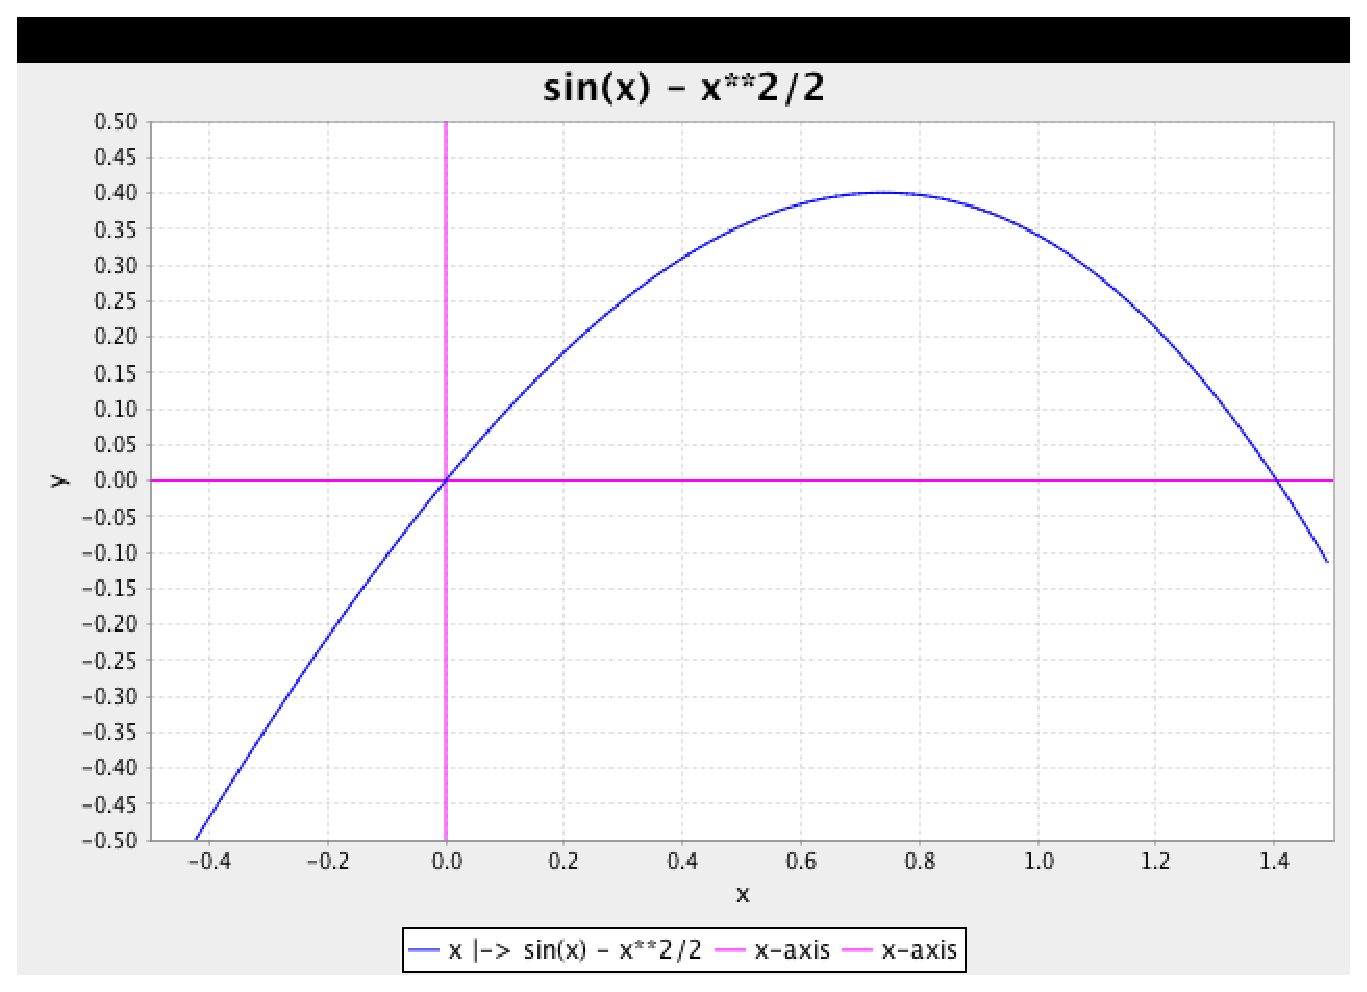
\epsfig{file=Figures/sin-minus-square.eps, scale=0.6}
\vspace*{-0.3cm}
\caption{The function $x \mapsto \sin(x) - \frac{1}{2} \cdot x^2$.}
\label{fig:sin-minus-square.eps}
\end{figure}

\noindent
Unfortunately, in many cases the equation 
\\[0.2cm]
\hspace*{1.3cm}
$\nabla f(\mathbf{\widehat{x}}) = \mathbf{0}$
\\[0.2cm]
can not be solved explicitly.  This is already true in the one-dimensional case, i.e.~if $n=1$.  For example, consider
the function $f:\mathbb{R} \rightarrow \mathbb{R}$ that is defined as
\\[0.2cm]
\hspace*{1.3cm}
$\ds f(x) := \sin(x) - \frac{1}{2} \cdot x^2$.
\\[0.2cm]
This function is shown in Figure \ref{fig:sin-minus-square.eps} on page \pageref{fig:sin-minus-square.eps}.
From the graph of the function it is obvious that this function has a maximum somewhere between $0.6$ and
$0.8$.  In order to compute this maximum, we can compute the derivative of $f$.   This derivative is given as 
\\[0.2cm]
\hspace*{1.3cm}
$f'(x) = \cos(x) - x$
\\[0.2cm]
As it happens, the equation $\cos(x) - x = 0$ does not seem to have a solution in 
\href{https://en.wikipedia.org/wiki/Closed-form_expression}{closed form}.  Hence, we can only approximate
the solution numerically.


The method of \href{https://en.wikipedia.org/wiki/Gradient_descent}{gradient ascent} is a numerical
method that can be used to find the maximum of a function 
\\[0.2cm]
\hspace*{1.3cm}
$f: \mathbb{R}^n \rightarrow \mathbb{R}$.
\\[0.2cm]
The basic idea is to take a vector $\mathbf{x}_0 \in \mathbb{R}^n$ as start value and define a sequence of
vectors $\bigl(\mathbf{x}_n\bigr)_{n\in\mathbb{N}}$ such that we have
\\[0.2cm]
\hspace*{1.3cm}
$f(\mathbf{x}_{n+1}) \geq f(\mathbf{x}_{n})$ \quad for all $n\in\mathbb{N}$.
\\[0.2cm]
Hopefully, this sequence will converge against $\widehat{\mathbf{x}} = \arg\max\limits_{\mathbf{x}\in \mathbb{R}^n}f(\mathbf{x})$.
If we do not really know where to start our search, we define $\mathbf{x}_0 := \mathbf{0}$.  In order to
compute $\mathbf{x}_{n+1}$ given $\mathbf{x}_{n}$, the idea is to move from $\mathbf{x}_n$ in that direction
where we have the biggest change in the values of $f$.   This direction happens to be the gradient of $f$ at $\mathbf{x}_n$.
Therefore, the definition of $\mathbf{x}_{n+1}$ is given as follows:
\\[0.2cm]
\hspace*{1.3cm}
$\mathbf{x}_{n+1} := \mathbf{x}_n + \alpha \cdot \nabla f(\mathbf{x}_n)$ \quad for all $n \in \mathbb{N}_0$.
\\[0.2cm]
Here, $\alpha$ is called the \blue{step size}.  It determines by how much we move in the direction of the gradient.
In practice, it is best to adapt the step size dynamically during the iteration.  Figure
\ref{fig:gradient-ascent.stlx} shows how this is done.



\begin{figure}[!ht]
\centering
\begin{Verbatim}[ frame         = lines, 
                  framesep      = 0.3cm, 
                  firstnumber   = 1,
                  labelposition = bottomline,
                  numbers       = left,
                  numbersep     = -0.2cm,
                  xleftmargin   = 0.8cm,
                  xrightmargin  = 0.8cm,
                ]
    findMaximum := procedure(f, gradF, start, eps) {
        x     := start;
        fx    := f(x);
        alpha := 1.0;
        while (true) {
            [xOld, fOld] := [x, fx];
            x  += alpha * gradF(x);
            fx := f(x);
            if (fx < fOld) {   
                alpha   *= 0.5;
                [x, fx] := [xOld, fOld];
                continue;  // start over
            } else {
                alpha *= 1.2;
            }
            if (abs(fx - fOld) <= abs(fx) * eps) {
                return [x, fx];
            } 
        }
    };
\end{Verbatim}
\vspace*{-0.3cm}
\caption{The gradient ascent algorithm.}
\label{fig:gradient-ascent.stlx}
\end{figure}

\noindent
The function \texttt{findMaximum} takes four arguments:
\begin{enumerate}
\item \texttt{f} is the function that is to be maximized.  It is assumed that \texttt{f} takes a vector
      $\texttt{x}\in \mathbb{R}^n$ as its input and that it returns a real number.
\item \texttt{gradF} is the gradient of \texttt{f}.  It takes a vector
      $\texttt{x}\in \mathbb{R}^n$ as its input and returns the vector $\nabla \mathtt{f}(\mathtt{x})$.
\item \texttt{start} is the a vector from $\mathbb{R}^n$ that is used as the value of $\mathbf{x}_0$.  In
      practice, we will often use $\mathbf{0} \in \mathbb{R}^n$ as the start vector.
\item \texttt{eps} is the precision that we need for the maximum.  We will have to say more on how \texttt{eps}
      is exactly related to the precision later.  As we are using double precision floating point arithmetic, 
      it won't make sense to use a value for \texttt{eps} that is smaller than $10^{-15}$.
\end{enumerate}
Next, let us discuss the implementation of gradient ascent.
\begin{enumerate}
\item \texttt{x} is initialized with the parameter \texttt{start}.  Hence, \texttt{start} is really the same as
      $\mathbf{x}_0$. 
\item \texttt{fx} is the value that the function $f$ takes for the argument \texttt{x}.
\item \texttt{alpha} is the step size $\alpha$.  We initialize \texttt{alpha} as $1.0$.  It will be adapted
      dynamically. 
\item The \texttt{while} loop starting in line 5 executes the iteration.
\item In each iteration, we store the values of $\mathbf{x}_n$ and $f(\mathbf{x}_n)$ in the variables
      \texttt{xOld} and \texttt{fOld}.
\item Next, we compute $\mathbf{x}_{n+1}$ in line 7 and compute the corresponding value $f(\mathbf{x}_{n+1})$ in line 8.
\item If we are unlucky, $f(\mathbf{x}_{n+1})$ is smaller than $f(\mathbf{x}_{n})$.  This happens if the step
      size $\alpha$ is too large.  Hence, in this case we decrease the value of $\alpha$, discard 
      both $\mathbf{x}_{n+1}$ and $f(\mathbf{x}_{n+1})$ and start over again.
\item Otherwise, $\mathbf{x}_{n+1}$ is a better approximation of the maximum than $\mathbf{x}_n$.  
      In order to increase the speed of the convergence of our algorithm we will then increase the step size
      $\alpha$ by $20\%$.    
\item The idea of our implementation is to stop the iteration when the function values of 
      $f(\mathbf{x}_{n+1})$ and $f(\mathbf{x}_{n})$ do not differ by more than $\varepsilon$ percent, or, to be more
      precise, if
      \\[0.2cm]
      \hspace*{1.3cm}
      $f(\mathbf{x}_{n+1}) < f(\mathbf{x}_{n}) \cdot (1 + \varepsilon)$.
      \\[0.2cm]
      As the sequence $\bigl(f(\mathbf{x}_n\bigr)_{n\in\mathbb{N}}$ will be monotonically
      increasing, i.e.~we have
      \\[0.2cm]
      \hspace*{1.3cm}
      $f(\mathbf{x}_{n+1}) \geq f(\mathbf{x}_{n})$ \quad for all $n\in\mathbb{N}$,
      \\[0.2cm]
      the condition given above is sufficient.  Now, if the increase of  $f(\mathbf{x}_{n+1})$ is less than $f(\mathbf{x}_{n}) \cdot (1 + \varepsilon)$ 
      we assume that we have reached the maximum with the required precision.  In this case we return both the
      value of \texttt{x} and the corresponding function value $f(\mathtt{x})$.
\end{enumerate}
The implementation of gradient ascent given above is not the most sophisticated variant of this algorithm.
It should also be noted that there are algorithms that are more powerful than
gradient ascent.  The first of these methods is the
\href{https://en.wikipedia.org/wiki/Conjugate_gradient_method}{conjugate gradient method}.  A
refinement of this method is the
\href{https://en.wikipedia.org/wiki/Broyden-Fletcher-Goldfarb-Shanno_algorithm}{BFGS-algorithm} that
has been invented by Broyden, Fletcher, Goldfarb, and Shanno.  Unfortunately, we do not have the
time to discuss this algorithm.
However, our implementation of gradient ascent is sufficient for our applications and as this is not a course on numerical
analysis but rather on artificial intelligence we will not delve deeper into this topic but, instead, we refer
readers interested in more efficient algorithms to the literature \cite{snyman:2005}.  If you ever need to find
the maximum of a function numerically, you should try to use a predefined library routine that implements a
state of the art algorithm.


\section{Logistic Regression}
In \href{https://en.wikipedia.org/wiki/Logistic_regression}{logistic regression} we use a linear model that is combined
with the \blue{sigmoid function}.  Before we can discuss the details of logistic regression we need to
define this function and state some of its properties. 

\subsection{The Simoid Function}
\begin{Definition}[Sigmoid Function]
The \href{https://en.wikipedia.org/wiki/Sigmoid_function}{sigmoid function} $S: \mathbb{R} \rightarrow [0, 1]$ is defined as 
\\[0.2cm]
\hspace*{1.3cm}
$\ds S(t) = \frac{1}{1 + \exp(-t)}$.  
\\[0.2cm]
Figure \ref{fig:sigmoid.eps} on page \pageref{fig:sigmoid.eps} shows the sigmoid function.
\eox
\end{Definition}

\begin{figure}[!ht]
\centering
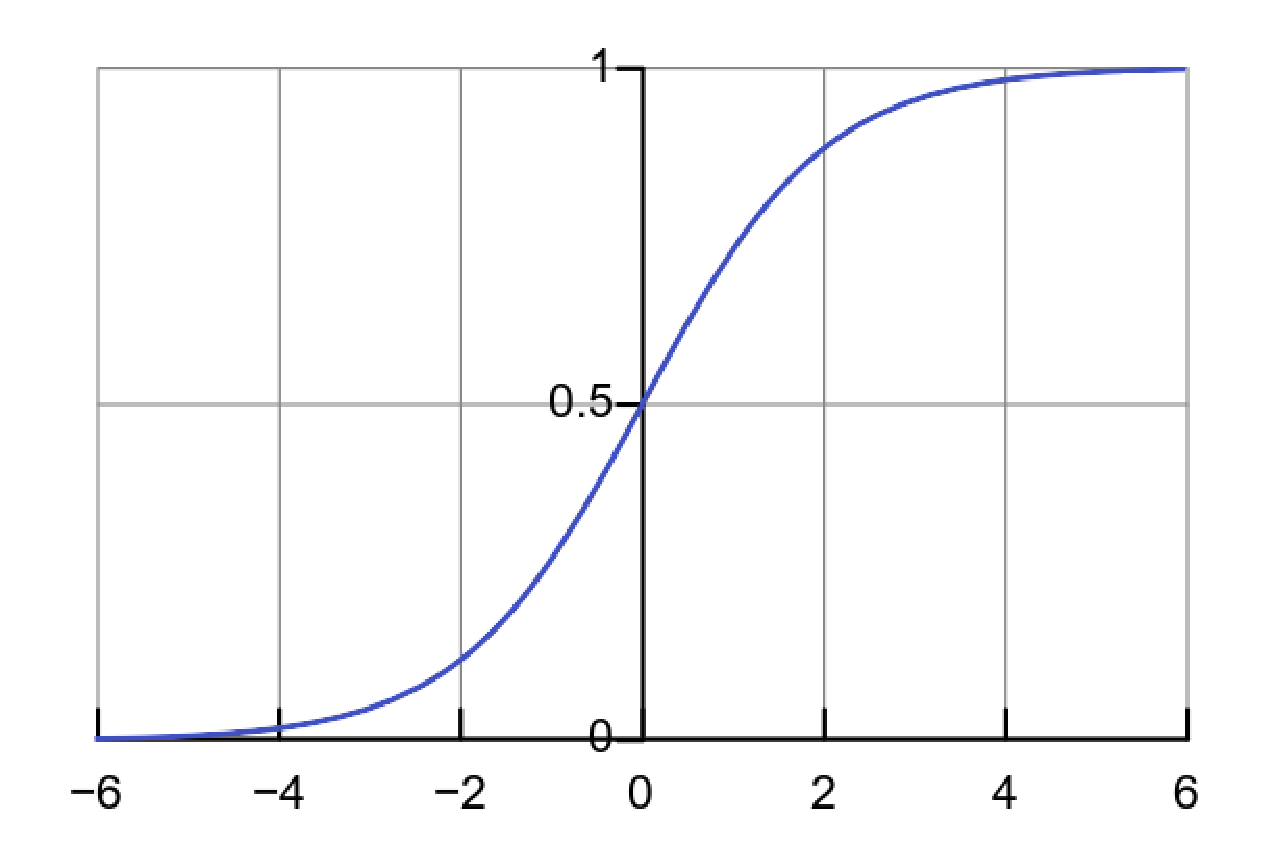
\epsfig{file=Figures/sigmoid.eps, scale=0.7}
\vspace*{-0.3cm}
\caption{The sigmoid function.}
\label{fig:sigmoid.eps}
\end{figure}


\noindent
Let us note some immediate consequences of the definition of the sigmoid function.  As we have
\\[0.2cm]
\hspace*{1.3cm}
$\ds\lim\limits_{x\rightarrow-\infty} \exp(-x) = \infty$, \quad 
$\ds\lim\limits_{x\rightarrow+\infty} \exp(-x) = 0$, \quad and \quad
$\ds\lim\limits_{x\rightarrow\infty} \frac{1}{x} = 0$, 
\\[0.2cm]
the sigmoid function has the following properties:
\\[0.2cm]
\hspace*{1.3cm}
$\ds \lim_{t\rightarrow-\infty} S(t) = 0$ \quad and \quad
$\ds \lim_{t\rightarrow+\infty} S(t) = 1$.
\\[0.2cm]
Another important property is the symmetry of the sigmoid function.  Figure \ref{fig:sigmoid.eps} shows that if the
sigmoid function is shifted down by $\frac{1}{2}$, the resulting function is 
\href{https://en.wikipedia.org/wiki/Point_reflection}{centrally symmetric}, i.e.~we have
\\[0.2cm]
\hspace*{1.3cm}
$\ds S(-t) - \frac{1}{2} = -\Bigl(S(t) - \frac{1}{2}\Bigr)$.
\\[0.2cm]
Adding $\ds\frac{1}{2}$ on both sides of this equation shows that this is equivalent to the equation
\\[0.2cm]
\hspace*{1.3cm}
\colorbox{red}{\framebox{\colorbox{orange}{
$S(-t) = 1 - S(t)$,}}}
\\[0.2cm]
The proof of this fact runs as follows:
\\[0.2cm]
\hspace*{1.3cm}
$
\begin{array}{lcll}
1 - S(t) & = & \ds 1 - \frac{1}{1 + \exp(-t)}             & \mbox{by definition of $S(t)$}           \\[0.5cm]
         & = & \ds \frac{1 + \exp(-t) - 1}{1 + \exp(-t)}  & \mbox{common denominator}                \\[0.5cm]
         & = & \ds \frac{\exp(-t)}{1 + \exp(-t)}          & \mbox{simplify}                          \\[0.5cm]
         & = & \ds \frac{1}{1 + \exp(+t)}                 & \mbox{expand fraction by $\exp(t)$}      \\[0.5cm]
         & = & S(-t). \qquad _\Box                         & \mbox{by definition of $S(-t)$}
\end{array}
$
\\[0.2cm]
The exponential function can be expressed via the sigmoid function.  Let us start with the definition of the sigmoid
function. 
\\[0.2cm]
\hspace*{1.3cm}
$\ds S(t) = \frac{1}{1 + \exp(-t)}$
\\[0.2cm]
Multiplying this equation with the denominator yields
\\[0.2cm]
\hspace*{1.3cm}
$\ds S(t) \cdot \bigl(1 + \exp(-t)\bigr) = 1$.
\\[0.2cm]
Dividing both sides by $S(t)$ gives:
\\[0.2cm]
\hspace*{1.3cm}
$
\begin{array}{cl}
                & \ds 1 + \exp(-t) = \frac{1}{S(t)}        \\[0.5cm]
\Leftrightarrow & \ds \exp(-t) = \frac{1}{S(t)} - 1        \\[0.5cm]
\Leftrightarrow & \ds \exp(-t) = \frac{1 - S(t)}{S(t)}      
\end{array}
$
\\[0.2cm]
We highlight this formula, as we need it later
\\[0.2cm]
\hspace*{1.3cm}
\colorbox{red}{\framebox{\colorbox{orange}{$\ds \exp(-t) = \frac{1 - S(t)}{S(t)}$.}}}
\\[0.2cm]
If we take the reciprocal of both sides of this equation, we have
\\[0.2cm]
\hspace*{1.3cm}
$\ds \exp(t) = \frac{S(t)}{1 - S(t)}$.
\\[0.2cm]
Applying the natural logarithm on both sides of this equation yields
\\[0.2cm]
\hspace*{1.3cm}
$\ds t = \ln\left(\frac{S(t)}{1-S(t)}\right)$.
\\[0.2cm]
This shows that the inverse of the sigmoid function is given as
\\[0.2cm]
\hspace*{1.3cm}
\colorbox{red}{\framebox{\colorbox{orange}{
$\ds S^{-1} (y) = \ln\left(\frac{y}{1-y}\right)$.}}} 
\\[0.2cm]
This function is known as the \href{https://en.wikipedia.org/wiki/Logit}{logit function}.
Next, let us compute the derivative of $S(t)$, i.e.~$\ds S'(t) =\frac{\mathrm{d}S}{\mathtt{d}t}$.  We have
\\[0.2cm]
\hspace*{1.3cm}
$
\begin{array}{lcl}
 S'(t) & = & \ds -\frac{-\exp(-t)}{\bigr(1+\exp(-t)\bigr)^2}   \\[0.5cm]
       & = & \ds \exp(-t) \cdot S(t)^2                       \\[0.2cm]
       & = & \ds \frac{1-S(t)}{S(t)} \cdot S(t)^2            \\[0.4cm]
       & = & \ds \bigl(1 - S(t)\bigr) \cdot S(t)            
\end{array}
$
\\[0.2cm]
We have shown
\\[0.2cm]
\hspace*{1.3cm}
\colorbox{red}{\framebox{\colorbox{orange}{$S'(t) = \bigl(1 - S(t)\bigr) \cdot S(t)$.}}}
\\[0.2cm]
We will later need the derivative of the logarithm of the logistic function.  We define
\\[0.2cm]
\hspace*{1.3cm}
$L(t) := \ln\bigl(S(t)\bigr)$.
\\[0.2cm]
Then we have
\\[0.2cm]
\hspace*{1.3cm}
$
\begin{array}{lcll}
  L'(t) & = & \ds \frac{S'(t)}{S(t)}                  & \mbox{by the chain rule} \\[0.5cm]
        & = & \ds \frac{(1 - S(t)) \cdot S(t)}{S(t)}  \\[0.5cm]
        & = & \ds 1 - S(t)                            \\[0.2cm]
        & = & \ds S(-t)
\end{array}
$
\\[0.2cm]
% If we have the function $f(t) := L(-t)$, then we see that
%\\[0.2cm]
%\hspace*{1.3cm}
% $f'(t) = -S(t)$
%\\[0.2cm]
% holds.   
As this is our most important result, we highlight it:
\\[0.2cm]
\hspace*{1.3cm}
\colorbox{red}{\framebox{\colorbox{orange}{$L'(t) = S(-t)$ \quad where \quad $L(t) := \ln\bigl(S(t)\bigr)$.}}}


\subsection{The Model of Logistic Regression}
We use the following model to compute the probability that an object with features $\mathbf{x}$ will be of the given class:
\\[0.2cm]
\hspace*{1.3cm}
$P(y=+1\;|\;\mathbf{x};\mathbf{w}) = S(\mathbf{x} \cdot \mathbf{w})$.
\\[0.2cm]
Here $\mathbf{x} \cdot \mathbf{w}$ denotes the dot product of the vectors $\mathbf{x}$ and $\mathbf{y}$.  It is
assumed that $\mathbf{x}$ contains a constant feature which  always takes the value of $1$.
Seeing this model the first time you might think that this model is not very general and that it can only be
applied in very special circumstances.  However, the fact is that the features can be functions of arbitrary complexity
and hence this model is much more general than it appears on first sight.

We assume that $y$ can only take the values $+1$ or $-1$,  e.g.~in the example of spam detection $y = 1$ if the
email is spam and $y = -1$ otherwise.  Since complementary probabilities add up to $1$, we have
\\[0.2cm]
\hspace*{1.3cm}
$P(y=-1\;|\;\mathbf{x};\mathbf{w}) = 1 - P(y=+1\;|\;\mathbf{x};\mathbf{w}) 
  = 1 - S(\mathbf{x} \cdot \mathbf{w}) = S(-\mathbf{x} \cdot \mathbf{w})
$.
\\[0.2cm]
Hence, we can combine the equations for $P(y=-1\;|\;\mathbf{x};\mathbf{w})$ and $P(y=+1\;|\;\mathbf{x};\mathbf{w})$ into a
single equation
\\[0.2cm]
\hspace*{1.3cm}
\colorbox{red}{\framebox{\colorbox{orange}{$P(y\;|\;\mathbf{x};\mathbf{w}) = S\bigl(y \cdot(\mathbf{x} \cdot \mathbf{w})\bigr)$.}}}
\\[0.2cm]
Given $N$ objects $o_1, \cdots, o_n $ with feature vectors $\mathbf{x}_1, \cdots, \mathbf{x}_n$ we
want to determine the weight vector $\mathbf{w}$ such that the likelihood $\ell(\mathbf{X}, \mathbf{y})$ of all of our
observations is maximized.  This approach is called the 
\href{https://en.wikipedia.org/wiki/Maximum_likelihood_estimation}{maximum likelihood estimation} of the weights.
As we assume the probabilities of different observations are independent, the individual
probabilities have to be multiplied to compute the overall likelihood $\ell(\mathbf{X}, \mathbf{y};\mathbf{w})$ 
of a given training set:
\\[0.2cm]
\hspace*{1.3cm}
$\ds \ell(\mathbf{X},\mathbf{y};\mathbf{w}) = \prod\limits_{i=1}^N P(y_i \;|\;\mathbf{x}_i;\mathbf{w})$.
\\[0.2cm]
Here, we have combined the different attribute vectors $\mathbf{x}_i$ into the matrix $\mathbf{X}$.  Since it is
easier to work with sums than with products, instead of maximizing the function $\ell(\mathbf{X},\mathbf{y};\mathbf{w})$ we maximize the function
\\[0.2cm]
\hspace*{1.3cm}
$\ell\ell(\mathbf{X},\mathbf{y};\mathbf{w}) := \ln\bigl(\ell(\mathbf{X},\mathbf{y};\mathbf{w})\bigr)$. 
\\[0.2cm]
As the natural logarithm is a monotone function, the functions $\ell(\mathbf{X},\mathbf{y};\mathbf{w})$ and 
$\ell\ell(\mathbf{X},\mathbf{y};\mathbf{w})$ take their maximum at the same value of $\mathbf{w}$.  As we have
\\[0.2cm]
\hspace*{1.3cm}
$\ln(a \cdot b) = \ln(a) + \ln(b)$,
\\[0.2cm]
the natural logarithm of the likelihood is 
\\[0.2cm]
\hspace*{1.3cm}
\colorbox{red}{\framebox{\colorbox{orange}{
$\ds \ell\ell(\mathbf{X},\mathbf{y};\mathbf{w}) = 
 \sum\limits_{i=1}^N \ln\Bigl(S\bigl(y_i \cdot(\mathbf{x}_i \cdot \mathbf{w})\bigr)\Bigr) =
 \sum\limits_{i=1}^N L\bigl(y_i \cdot(\mathbf{x}_i \cdot \mathbf{w})\bigr)
$.}}}
\\[0.2cm]
Our goal is to maximize the likelihood.  Since this is the same as maximizing the log-likelihood, we
need to determine those values of the coefficients $\mathbf{w}$ that satisfy
\\[0.2cm]
\hspace*{1.3cm}
$\ds \frac{\partial\quad}{\partial\, w_j}\ell\ell(\mathbf{X},\mathbf{y};\mathbf{w}) = 0$.
\\[0.2cm]
In order to compute the partial derivative of $\ell\ell(\mathbf{X},\mathbf{y};\mathbf{w})$ with respect to the
coefficients $\mathbf{w}$ we need to compute the partial derivative of the dot product $\mathbf{x}_i \cdot
\mathbf{w}$ with respect to the weights $w_j$.
We define
\\[0.2cm]
\hspace*{1.3cm}
$\ds h(\mathbf{w}) := \mathbf{x}_i \cdot \mathbf{w} = \sum\limits_{k=1}^D x_{i,k} \cdot w_j$.
\\[0.2cm]
Then we have
\\[0.2cm]
\hspace*{1.3cm}
$\ds \frac{\partial\quad}{\partial\, w_j} h(\mathbf{w}) = x_{i,j}$.
\\[0.2cm]
Now we are ready to compute the partial derivative of $\ell\ell(\mathbf{X},\mathbf{y};\mathbf{w})$ with respect to $\mathbf{w}$:
\\[0.2cm]
\hspace*{1.3cm}
$
\begin{array}{cll}
  & \ds \frac{\partial\quad}{\partial\, w_j} \ell\ell(\mathbf{X},\mathbf{y};\mathbf{w}) \\[0.5cm]
= & \ds \frac{\partial\quad}{\partial\, w_j} 
    \sum\limits_{i=1}^N L\bigl(y_i \cdot(\mathbf{x}_i \cdot \mathbf{w})\bigr) 
    \\[0.5cm]
= & \ds\sum\limits_{i=1}^N y_i \cdot x_{i,j} \cdot  S\bigl(-y_i \cdot(\mathbf{x}_i \cdot \mathbf{w})\bigr),
  & \mbox{since} \quad \ds \frac{\mathrm{d}L(x)}{\mathrm{d}x} = S(-x).
\end{array}
$
\\[0.2cm]
Hence, the partial derivative of the log-likelihood function is given as follows:
\\[0.2cm]
\hspace*{1.3cm}
\colorbox{red}{\framebox{\colorbox{orange}{
$\ds \frac{\partial\quad}{\partial\, w_j}\ell\ell(\mathbf{X},\mathbf{y};\mathbf{w}) =
 \ds\sum\limits_{i=1}^N y_i \cdot x_{i,j} \cdot  S(-y_i \cdot \mathbf{x}_i \cdot \mathbf{w})
$}}} 
\\[0.2cm]
Next, we have to find the value of $\mathbf{w}$ such that
\\[0.2cm]
\hspace*{1.3cm}
$\ds\sum\limits_{i=1}^N y_i \cdot x_{i,j} \cdot  S(-y_i \cdot \mathbf{x}_i \cdot \mathbf{w}) = 0$
\quad for all $j \in \{1, \cdots, D\}$.
\\[0.2cm]
These are $D$ equation for the $D$ variables $w_1, \cdots w_D$.  Due to the occurrence of the sigmoid function, these
equations are nonlinear.  We can not solve these equations explicitly.  Nevertheless, our computation of the
gradient of the log-likelihood was not for nought:  We will use gradient ascent in order to find the value of
$\mathbf{w}$ that maximizes the log-likelihood.
This method has been outlined in the previous section.

\subsection{Implementing Logistic Regression}
In order to implement logistic regression we need a data structure for tabular data.  Figure
\ref{fig:table.stlx} on page \pageref{fig:table.stlx} shows the class table that can be used to
administer this kind of data.  Figure \ref{fig:table.stlx}  shows an example of tabular data that is
stored in a \href{https://en.wikipedia.org/wiki/Comma-separated_values}{csv file}.  In this case,
the data stores the hours a student has learned for a particular exam and the fact whether the
student has passed of failed.  The first column stores pass or fail, where a pass is coded using the
number 1, while a fail is coded as 0.  The second column stores the number of hours that the student
has learned in order to pass the exam.

\begin{figure}[!ht]
\centering
\begin{Verbatim}[ frame         = lines, 
                  framesep      = 0.3cm, 
                  firstnumber   = 1,
                  labelposition = bottomline,
                  numbers       = left,
                  numbersep     = -0.2cm,
                  xleftmargin   = 0.8cm,
                  xrightmargin  = 0.8cm,
                ]
   class table(columnNames, types, data) {
       mColumnNames := columnNames;
       mTypes       := types;
       mData        := data;
   
     static {
         getColumnNames := [ ] |-> mColumnNames;
         getTypes       := [ ] |-> mTypes;
         getData        := [ ] |-> mData;
         getRow         := [r] |-> mData[r];
         getLength      := []  |-> #mData;
         
         head := procedure(limit := 10) {
             print(mColumnNames);
             print(mTypes);
             for (i in [1 .. limit]) {
                 print(mData[i]);
             }
         };
     }
   }
   readTable := procedure(fileName, types) {
       all := readFile(fileName);
       columnNames := split(all[1], ',\s*');
       data := [];
       for (i in [2 .. #all]) {
           row := split(all[i], ',\s*');
           data[i-1] := [eval("$type$($s$)") : [type, s] in types >< row];
       }
       return table(columnNames, types, data);
   };
\end{Verbatim}
\vspace*{-0.3cm}
\caption{A class to represent tabular data.}
\label{fig:table.stlx}
\end{figure}
There is no need for us to discuss every detail of the implementation of the class \texttt{table}.
The important thing to note is that the data is stored as a list of lists in the member variable
\texttt{mData}.  Each of the inner lists corresponds to one row of the csv file.
This member variable can be accessed using the function getData.  The function \texttt{readTable}
has the responsibility to read a csv file and to convert it into an object of class \texttt{table}.
In order to do this, it has to be called with two arguments.  The first argument is the file name,
the second argument is a list of the types of each column in the csv file.  For example, to read the
file ``\texttt{exam.csv}'' we would call \texttt{readTable} as follows:
\\[0.2cm]
\hspace*{1.3cm}
\texttt{readTable("exam.csv", ["int", "double"])}.



\begin{figure}[!ht]
\centering
\begin{Verbatim}[ frame         = lines, 
                  framesep      = 0.3cm, 
                  firstnumber   = 1,
                  labelposition = bottomline,
                  numbers       = left,
                  numbersep     = -0.2cm,
                  xleftmargin   = 0.8cm,
                  xrightmargin  = 0.8cm,
                ]
   Pass, Hours
   0,    0.50
   0,    0.75
   0,    1.00
   0,    1.25
   0,    1.50
   0,    1.75
   1,    1.75
   0,    2.00
   1,    2.25
   0,    2.50
   1,    2.75
   0,    3.00
   1,    3.25
   0,    3.50
   1,    4.00
   1,    4.25
   1,    4.50
   1,    4.75
   1,    5.00
   1,    5.50
\end{Verbatim}
\vspace*{-0.3cm}
\caption{Results of an exam.}
\label{fig:exam.csv}
\end{figure}

The program shown in Figure \ref{fig:logistic-regression.stlx} on page
\pageref{fig:logistic-regression.stlx} implements logistic regression.  As there are a number of
subtle points that might easily be overlooked otherwise, we proceed to discuss this program line by line. 


\begin{figure}[!ht]
\centering
\begin{Verbatim}[ frame         = lines, 
                  framesep      = 0.3cm, 
                  firstnumber   = 1,
                  labelposition = bottomline,
                  numbers       = left,
                  numbersep     = -0.2cm,
                  xleftmargin   = 0.8cm,
                  xrightmargin  = 0.8cm,
                ]
   load("table.stlx");
   load("gradient-ascent.stlx");
   
   sigmoid := procedure(x) { return 1.0 / (1.0 + exp(-x)); };
   logSigmoid := procedure(x) {
       if (x >= -100) {
           return -log(1.0 + exp(-x));
       } else {  
           return x;
       }
   };
   ll := procedure(X, y, w) {
       result := 0;
       for (i in [1 .. #X]) {
           result += logSigmoid(y[i] * (X[i] * w));
       }
       return result;
   };   
   gradLL := procedure(X, y, w) {
       result := [];
       for (j in [1 .. #X[1]]) {
           result[j] := 0;
           for (i in [1 .. #X]) {
               result[j] += y[i] * X[i][j] * sigmoid((-y[i]) * (X[i] * w));
           }
       }
       return la_vector(result);
   };
   logisticRegressionFile := procedure(fileName, types) {
       csv    := readTable(fileName, types);
       data   := csv.getData();
       number := #data;
       dmnsn  := #data[1];    
       yList  := [];
       xList  := [];
       for (i in [1 .. number]) {
           yList[i] := data[i][1];
           xList[i] := la_vector([1.0] + data[i][2..]);
       }
       X := la_matrix(xList);
       y := la_vector([2 * y - 1 : y in yList]);
       start := la_vector([0.0 : i in [1 .. dmnsn]]);
       eps   := 10 ** -15;
       f     := w |=> ll(X, y, w);
       gradF := w |=> gradLL(X, y, w);
       return findMaximum(f, gradF, start, eps)[1];
   };
\end{Verbatim}
\vspace*{-0.3cm}
\caption{An implementation of logistic regression.}
\label{fig:logistic-regression.stlx}
\end{figure}

\begin{enumerate}
\item First, we have to load both the class \texttt{table} and our implementation of gradient ascent 
      that has already been discussed in Section \ref{section:gradient-ascent}.
\item Line 4 implements the sigmoid function
      \\[0.2cm]
      \hspace*{1.3cm}
      $\ds S(x) = \frac{1}{1 + \exp(-x)}$.
\item Line 5 starts the implementation of the natural logarithm of the sigmoid function, i.e.~we implement
      \\[0.2cm]
      \hspace*{1.3cm}
      $\ds L(x) = \ln\bigl(S(X)\bigr) = \ln\left(\frac{1}{1 + \exp(-x)}\right) =- \ln\bigl(1 + \exp(-x)\bigr)$.
      \\[0.2cm]
      The implementation is more complicated than you might expect.  The reason has to do with
      overflow.  Consider values of $x$ that are smaller than, say, $-1000$.  The problem is that
      the expression $\mathtt{exp}(1000))$ evaluates to \texttt{Infinity}, which represents the
      mathematical value $\infty$.  But then $1 + \mathtt{exp}(1000))$ is also \texttt{Infinity} and
      finally \texttt{log(1 + exp(1000))} is \texttt{Infinity}.  However, in reality we have
      \\[0.2cm]
      \hspace*{1.3cm}
      $\ln\bigl(1 + \exp(1000)\bigr) \approx 1000$.
      \\[0.2cm] 
      The argument works as follows:
      \pagebreak
      \vspace*{\fill}

      \pagebreak

      \noindent
      \hspace*{1.3cm}
      $
      \begin{array}{lcll}
        \ln\bigl(1+\exp(x)\bigr) & = & \ln\bigl(\exp(x) \cdot (1+\exp(-x))\bigr)          \\[0.2cm]
                                 & = & \ln\bigl(\exp(x)\bigr) + \ln\bigl(1+\exp(-x)\bigr) \\[0.2cm]
                                 & = & x + \ln\bigl(1+\exp(-x)\bigr) \\[0.2cm]
                                 & \approx & x + \ln(1) + \exp(-x) & \mbox{Taylor expansion of $\ln(1+x)$} \\[0.2cm]
                                 & = & x + 0 + \exp(-x)                                      \\[0.2cm]
                                 & \approx & x                & \mbox{since $\exp(-x) \approx 0$ for large $x$} 
      \end{array}
      $
      \\[0.2cm]
      This is the reason that \texttt{logSigmoid} returns \texttt{x} if \texttt{x} is less than
      $-100$.
\item The function $\mathtt{ll}(\mathbf{x}, \mathbf{y}, \mathbf{w})$ computes the log-lokelihood
      $\ds \ell\ell(\mathbf{X},\mathbf{y};\mathbf{w}) = 
           \sum\limits_{i=1}^N L\bigl(y_i \cdot(\mathbf{x}_i \cdot \mathbf{w})\bigr)
      $.
      Here $L$ denotes the natural logarithm of the sigmoid of the argument.
      It is assumed that $\mathbf{X}$ is a matrix.  Every observation corresponds to a row in this
      matrix, i.e.~the vector $\mathbf{x}_i$ is the feature vector containing the features of the
      $i$-th observation.  $\mathbf{y}$ is a vector describing the outcomes, i.e.~the elements
      of this vector are either $+1$ or $-1$.  Finally, $\mathbf{w}$ is the vector of coefficients.
\item The function $\mathtt{gradLL}(\mathbf{x}, \mathbf{y}, \mathbf{w})$ computes the gradient of
      the log-lokelihood according to the formula
      \\[0.2cm]
      \hspace*{1.3cm}
      $\ds \frac{\partial\quad}{\partial\, w_j}\ell\ell(\mathbf{X},\mathbf{y};\mathbf{w}) =
        \ds\sum\limits_{i=1}^N y_i \cdot x_{i,j} \cdot  S(-y_i \cdot \mathbf{x}_i \cdot \mathbf{w})
      $.
      \\[0.2cm]
      The different components of this gradient are combined into a vector.
      The arguments are the same as the arguments to the log-lokelihood.
\item Finally, the function \texttt{logisticRegressionFile} takes two arguments.  The first argument
      is the name of the csv file containing the data, while the second argument is a list specifying the types
      of the columns.  The elements of this list have to be either \texttt{"int"} or
      \texttt{"double"}.
      The task of this function is to read the csv file, convert the data in the matrix $\mathbf{X}$
      and the vector $\mathtt{y}$, and then use the method of gradient ascent to find the coefficients
      $\mathtt{w}$ that maximize the likelihood.
\end{enumerate}
If we run the function \texttt{logisticRegressionFile} using the data shown in Figure
\ref{fig:exam.csv} via
the command
\\[0.2cm]
\hspace*{1.3cm}
\texttt{logisticRegressionFile("exam.csv", ["int", "double"]);}
\\[0.2cm]
the resulting coefficients are:
\\[0.2cm]
\hspace*{1.3cm}
\texttt{<<-4.077649741107752 1.5046211108850898>>}
\\[0.2cm]
This shows that the probability $P(h)$ that a student who has studied for $h$ hours will pass the
exam is given approximately as follows:
\\[0.2cm]
\hspace*{1.3cm}
$\ds P(h) \approx \frac{1}{1 + \exp(4.1 - 1.5 \cdot h)}$
\\[0.2cm]
Figure \ref{fig:exam-pass.eps} shows a plot of the probability $P(x)$.  This
figure has been taken from the
\href{https://en.wikipedia.org/wiki/Logistic_regression#Fields_and_example_applications}{Wikipedia article on logistic regression}. 
It has been created by \href{https://commons.wikimedia.org/w/index.php?curid=42442194}{Michaelg2015}.


\begin{figure}[!th]
\centering
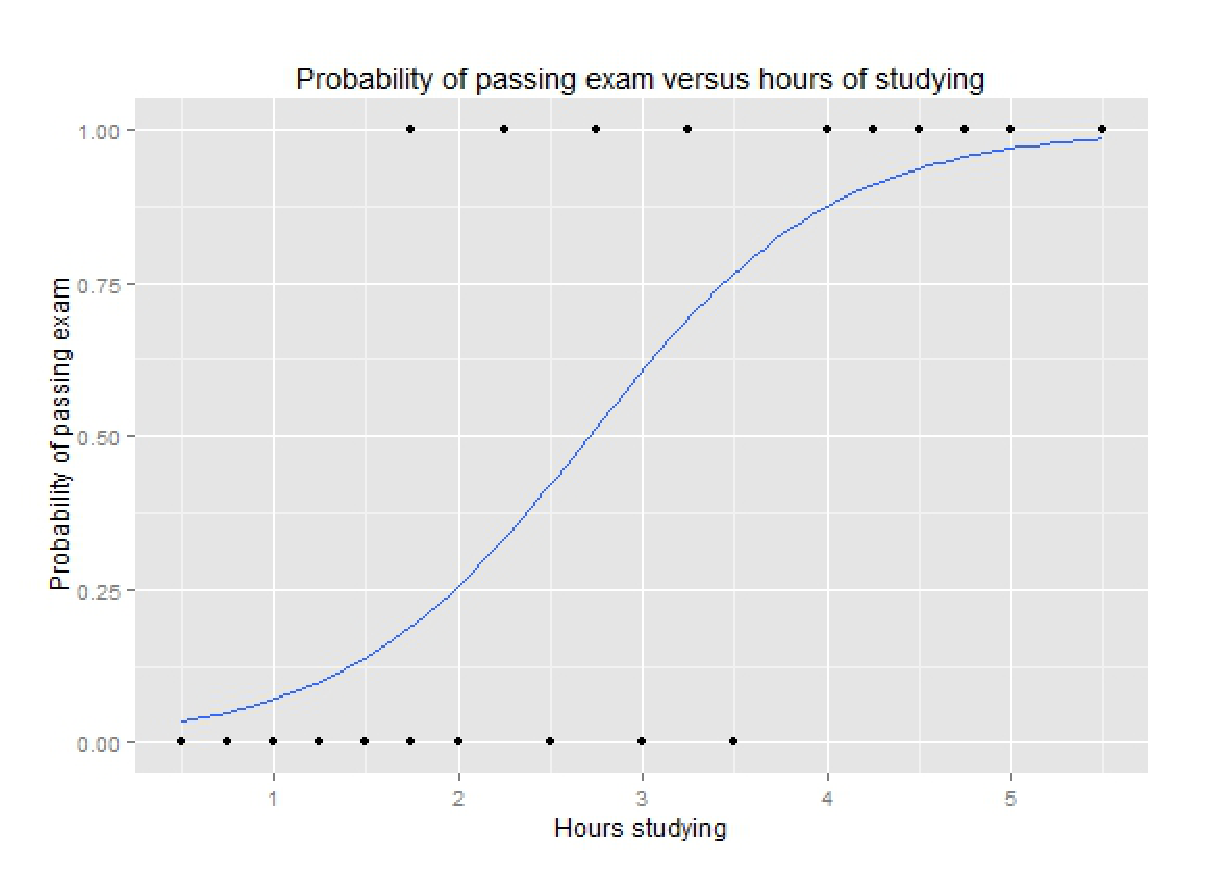
\epsfig{file=Figures/exam-pass.eps, scale=0.6}
\vspace*{-0.3cm}
\caption{Probability of passing an exam versus hours of studying.}
\label{fig:exam-pass.eps}
\end{figure}


%\section{Decision Tree Learning}

%%% Local Variables:
%%% mode: latex
%%% TeX-master: "artificial-intelligence"
%%% End:

% \chapter{Neural Networks}
In this chapter, we discuss \href{https://en.wikipedia.org/wiki/Artificial_neural_network}{neural networks}.
Many of the most visible breakthroughs in artificial intelligence have been achieved through the use of neural
networks: 
\begin{enumerate}
\item The current system used by Google to \href{https://translate.google.com}{automatically translate} web
      pages is called 
      ``\href{https://en.wikipedia.org/wiki/Google_Neural_Machine_Translation}{Google Neural Machine
        Translation}''
      and,  as the name suggests, is based on neural networks.  
\item \href{https://de.wikipedia.org/wiki/AlphaGo}{AlphaGo} uses neural networks together with tree search
      \cite{silver:2016}.  It has \href{https://en.wikipedia.org/wiki/AlphaGo_versus_Lee_Sedol}{recently} 
      beaten \href{https://en.wikipedia.org/wiki/Lee_Sedol}{Lee Sedol} in the game of go.  At that time, Lee Sedol was
      ranked third among the \href{https://www.goratings.org/history/}{top go players}. 
\item \href{https://en.wikipedia.org/wiki/Autonomous_car}{Autonomous driving} makes heavy use of neural networks.
\end{enumerate}
The list given above is far from being complete.  In this chapter, we will only discuss \blue{feedforward} 
neural networks.  Although recently 
\href{https://en.wikipedia.org/wiki/Recurrent_neural_network}{recurrent neural networks} have gotten a lot of
attention, these type of neural networks are more difficult to train and are therefore beyond the scope of this
introduction.  The rest of this chapter is strongly influenced by the online book 
\\[0.2cm]
\hspace*{1.3cm}
\href{http://neuralnetworksanddeeplearning.com/index.html}{http://neuralnetworksanddeeplearning.com/index.html}
\\[0.2cm]
that has been written by Michael Nielsen \cite{nielsen:2015}.  This book is easy to read, carefully written, and
free to access.  I recommend this book to anybody who wants to dive deeper into the fascinating topic of neural
networks.

\section{Feedforward Neural Networks}
A neural network is built from \blue{neurons}.  Neural networks are inspired by biological 
\href{https://en.wikipedia.org/wiki/Neuron}{neurons}.  However, in order to understand artificial neural
networks it is not necessary to know how biological neurons work and it is definitely not necessary to
understand how networks of biological neurons, i.e.~brains, work\footnote{
  Actually, when it comes to brains, although there are many speculations, surprisingly little is known for a fact.  
}.  
Instead, we develop a mathematical
abstraction of neurons that will serve as the foundation of the theory developed in this chapter.
At the abstraction level that we are looking at neural networks, a single neuron with $n$ inputs is defined as
a pair $\langle \mathbf{w}, b\rangle$ where the 
vector $\mathbf{w} \in \mathbb{R}^m$ is called the \blue{weight vector} and the number $b \in \mathbb{R}$ is called the \blue{bias}.  
Conceptually, a neuron is a function $p$ that maps an input vector $\mathbf{x} \in \mathbb{R}^m$ into the
interval $[0,1]$.  This function is defined as follows:
\\[0.2cm]
\hspace*{1.3cm}
$\ds p(\mathbf{x}; \mathbf{w}, b) := a(\mathbf{x} \cdot \mathbf{w} + b)$,
\\[0.2cm]
where $a$ is called the \blue{activation function}.  In our applications, we will always use the sigmoid
function as our activation function, i.e.~we have
\\[0.2cm]
\hspace*{1.3cm}
$\ds a(t) := S(t) = \frac{1}{1 + \exp(-t)}$.
\\[0.2cm]
The function $p$ modelling the neuron can be written more explicitly using index notation.  If
\\[0.2cm]
\hspace*{1.3cm}
$\mathbf{w} = \langle w_1, \cdots, w_m \rangle^\top$ 
\\[0.2cm]
is the weight vector and 
\\[0.2cm]
\hspace*{1.3cm}
$\mathbf{x} = \langle x_1, \cdots, x_m \rangle^\top$
\\[0.2cm]
is the input vector, then we have
\\[0.2cm]
\hspace*{1.3cm}
$\ds p(\mathbf{x}; \mathbf{w}, b) = S\left(\biggl(\sum\limits_{i=1}^m x_i \cdot w_i\biggr) + b\right)$.
\\[0.2cm]
If we compare $p(\mathbf{x}; \mathbf{w}, b)$ 
to a similar function appearing in the last chapter, you will notice 
that so far a neuron works just like logistic regression.  The only difference is that the bias $b$
is now explicit in our notation.  In logistic regression, we had assumed that the first component $x_1$ of our
feature vector $\mathbf{x}$ was always equal to $1$.  This assumption enabled us to incorporate the bias $b$ into the
weight vector $\mathbf{w}$.

A \blue{feedforward neural network} is a layered network of neurons.  Formally, the \blue{topology} of a neural network is
given by a number $L \in \mathbb{N}$ and a list $[m(1), \cdots, m(L)]$ of $L$ natural numbers.  The number
$L$ is called the \blue{number of layers} and for $i \in \{2,\cdots,L\}$ the number $m(i)$ is the number of
neurons in the $l$-th layer.  The first layer is called the \blue{input layer}.  The input layer does not contain
neurons but instead just contains \blue{input nodes}.  The last layer (i.e.~the
layer with index $L$) is called the \blue{output layer} and the remaining layers are called 
\blue{hidden layers}.  If there is more than one hidden layer, the neural network is called a
\blue{deep neural network}.

As the first layer is the input layer, the \blue{input dimension} is defined as
$m(1)$.  Similarly, the \blue{output dimension} is defined as $m(L)$.
Every node in the $l$-th layer is connected to every node in the $(l+1)$-th layer via a \blue{weight}.
The weight $w_{j,k}^{(l)}$ is the weight of the connection from the $k$-th neuron in layer $l-1$ to
the $j$-th neuron in layer $l$.  The weights in layer $l$ are combined into the \blue{weight matrix} $W^{(l)}$ of
the layer $l$: This matrix is defined as
\\[0.2cm]
\hspace*{1.3cm}
$\ds W^{(l)} := \bigl( w_{j,k}^{(l)} \bigr)$.
\\[0.2cm]
Note that $W^{(l)}$ is an $m(l) \times m(l-1)$ matrix, i.e.~we have
\\[0.2cm]
\hspace*{1.3cm}
$\ds W^{(l)} \in \mathbb{R}^{m(l) \times m(l-1)}$.
\\[0.2cm]
The $j$-th neuron in layer $l$ has the \blue{bias} $b_j^{(l)}$.  These biases of layer $l$ are combined into
the \blue{bias vector}
\\[0.2cm]
\hspace*{1.3cm}
$\mathbf{b}^{(l)} := \langle b_1^{(l)}, \cdots, b_{m(l)}^{(l)} \rangle^\top$.
\\[0.2cm]
Then, the \blue{activation} of the $j$-th neuron
in layer $l$ is denoted as $a_j^{(l)}$ and is defined recursively as follows:
\begin{enumerate}
\item For the input layer we have
      \begin{equation}
        \label{eq:feedforward1}
       a^{(1)}_j := x_j.
       \tag{FF1}
      \end{equation}
      To put it differently, the input vector $\mathbf{x}$ is the activation of the input nodes.
\item For all other layers we have
      \begin{equation}
         \label{eq:feedforward2}
         a_j^{(l)}(\mathbf{x}) := 
             S\left(\Biggl(\sum\limits_{k=1}^{m(l-1)} w_{j,k}^{(l)}\cdot a_k^{(l-1)}(\mathbf{x})\Biggr) + b_{j}^{(l)}\right) 
        \quad \mbox{for all $l \in \{2, \cdots, L\}$}.
       \tag{FF2}
\end{equation}
\end{enumerate}
The \blue{activation vector} of layer $l$ is defined as
\\[0.2cm]
\hspace*{1.3cm}
$\mathbf{a}^{(l)} := \langle a_1^{(l)}, \cdots, a_{m(l)}^{(l)} \rangle^\top$.
\\[0.2cm]
The output of our neural network for an input $\mathbf{x}$ is given by the neurons in the output
layer,  i.e.~the output vector 
$\mathbf{o}(\mathbf{x}) \in \mathbb{R}^{m(L)}$ is defined as 
\\[0.2cm]
\hspace*{1.3cm}
$\mathbf{o}(\mathbf{x}) := \langle a^{(L)}_1(\mathbf{x}), \cdots, a^{(L)}_{m(L)}(\mathbf{x}) \rangle^\top = \mathbf{a}^{(L)}(\mathbf{x})$.
\\[0.2cm]
Note that the equations (\ref{eq:feedforward1}) and (\ref{eq:feedforward2}) describe how information propagates
through the neural network: 
\begin{enumerate}
\item Initially, the input vector $\mathbf{x}$ is given and stored in the input layer of the neural network:
      \\[0.2cm]
      \hspace*{1.3cm}
      $\mathbf{a}^{(1)}(\mathbf{x}) := \mathbf{x}$.
\item The first layer of neurons, which is the second layer of nodes,  is activated and computes the activation
      vector $\mathbf{a}^{(2)}$ according to the formula
      \\[0.2cm]
      \hspace*{1.3cm}
      $\mathbf{a}^{(2)}(\mathbf{x}) := S\bigl(W^{(2)} \cdot \mathbf{a}^{(1)}(\mathbf{x}) + \mathbf{b}^{(2)}\bigr) = 
                                        S\bigl(W^{(2)} \cdot \mathbf{x} + \mathbf{b}^{(2)}\bigr)
      $.
\item The second layer of neurons, which is the third layer of nodes,  is activated and computes the activation
      vector $\mathbf{a}^{(3)}(\mathbf{x})$ according to the formula
      \\[0.2cm]
      \hspace*{1.3cm}
      $\mathbf{a}^{(3)}(\mathbf{x}) := S\bigl(W^{(3)} \cdot \mathbf{a}^{(2)}(\mathbf{x}) + \mathbf{b}^{(3)}\bigr)
                          = S\Bigl(W^{(3)} \cdot S\bigl(W^{(2)} \cdot \mathbf{x} + \mathbf{b}^{(2)}\bigr) + \mathbf{b}^{(1)}\Bigr)
        $
\item This proceeds until the output layer is reached and the output
      \\[0.2cm]
      \hspace*{1.3cm}
      $\mathbf{o}(\mathbf{x}) := \mathbf{a}^{(L)}(\mathbf{x})$
      \\[0.2cm]
      has been computed.  Note that very neuron of the neural network performs logistic regression.
\end{enumerate}
Next, we assume that we have $n$ \blue{training examples} 
\\[0.2cm]
\hspace*{1.3cm}
$\langle \mathbf{x}^{(i)}, \mathbf{y}^{(i)} \rangle$ \quad for $i=1,\cdots,n$ 
\\[0.2cm]
such that 
\\[0.2cm]
\hspace*{1.3cm}
$\mathbf{x}^{(i)} \in \mathbb{R}^{m(1)}$ and $\mathbf{y}^{(i)} \in \mathbb{R}^{m(L)}$
\\[0.2cm]
Our goal is to choose the weight matrices $W^{(l)}$ and the bias vectors $b^{(l)}$ in a way such that
\\[0.2cm]
\hspace*{1.3cm}
$\mathbf{o}\bigl(\mathbf{x}^{(i)}\bigr) = \mathbf{y}^{(i)}$ \quad for all $i \in \{1,\cdots,n\}$.
\\[0.2cm]
Unfortunately, in general we will not be able to achieve equality for all  $i \in \{1,\cdots,n\}$.
Therefore, our goal is to minimize the \blue{error} instead.  To be more precise, the 
\blue{quadratic error cost function} is defined as 
\\[0.2cm]
\hspace*{1.3cm}
$\ds C\Bigr(W^{(2)}, \cdots, W^{(L)}, \mathbf{b}^{(2)}, \cdots, \mathbf{b}^{(L)};
     \mathbf{x}^{(1)}, \mathbf{y}^{(1)}, \cdots, \mathbf{x}^{(n)},\mathbf{y}^{(n)} \Bigr) := 
 \frac{1}{2 \cdot n} \cdot \sum\limits_{i=1}^n \Bigl(\mathbf{o}\bigl(\mathbf{x}^{(i)}\bigr) - \mathbf{y}^{(i)}\Bigr)^2
$.
\\[0.2cm]
Note that the cost function is additive in the training examples $\langle \mathbf{x}^{(i)}, \mathbf{y}^{(i)} \rangle$.
In order to simplify the notation we define
\\[0.2cm]
\hspace*{1.3cm}
$\ds C_{\mathbf{x}, \mathbf{y}}\Bigr(W^{(2)}, \cdots, W^{(L)}, \mathbf{b}^{(2)}, \cdots, \mathbf{b}^{(L)}\Bigr) := 
 \frac{1}{2} \cdot \Bigl(\mathbf{a}^{(L)}\bigl(\mathbf{x}\bigr) - \mathbf{y}\Bigr)^2
$,
\\[0.2cm]
i.e.~$C_{\mathbf{x},\mathbf{y}}$ is the part of the cost function that is associated with a single training example $\pair(\mathbf{x},\mathbf{y})$.
Then, we have
\\[0.2cm]
$\ds C\Bigr(W^{(2)}, \cdots, W^{(L)}, \mathbf{b}^{(2)}, \cdots, \mathbf{b}^{(L)};
     \mathbf{x}^{(1)}, \mathbf{y}^{(1)}, \cdots, \mathbf{x}^{(n)},\mathbf{y}^{(n)} \Bigr) := 
 \frac{1}{n} \cdot \sum\limits_{i=1}^n C_{\mathbf{x^{(i)}}, \mathbf{y}^{(i)}}\Bigr(W^{(2)}, \cdots W^{(L)}, \mathbf{b}^{(2)}, \cdots, \mathbf{b}^{(L)}\Bigr) 
$.
\\[0.2cm]
As the notation
\\[0.2cm]
\hspace*{1.3cm}
$C_{\mathbf{x}, \mathbf{y}}\Bigr(W^{(2)}, \cdots, W^{(L)}, \mathbf{b}^{(2)}, \cdots, \mathbf{b}^{(L)}\Bigr)$
\\[0.2cm]
is far too heavy, we will abbreviate this term as $C_{\mathbf{x}, \mathbf{y}}$ in the following
discussion of the backpropagation algorithm.  Similarly, we abbreviate the quadratic error cost function as $C$.
Our goal is to choose the weight matrices $W^{(l)}$ and the bias vectors $\mathbf{b}^{(l)}$ such that the
quadratic error cost function $C$ is minimized.  We will use a variation of gradient descent to
find this minimum\footnote{
  In logistic regression we have tried to \emph{maximize} the log-likelihood.  Here, instead
  we \emph{minimize} the quadratic error cost function.  Hence, instead of gradient \emph{ascent} we use
  gradient \emph{descent}.  
}.
\pagebreak

\section{Backpropagation}
There are two reasons for the recent success of neural networks.
\begin{enumerate}
\item The computing power that is available today has vastly increased in the last 20 years.
      For example, today the \href{https://en.wikipedia.org/wiki/AMD_Radeon_400_series#Vega}{AMD Vega 10}
      graphic card offers about 12.5 teraflops in single precision performance.  It consumes about 300 watt.
      Contrast this with \href{https://en.wikipedia.org/wiki/ASCI_White}{ASCI White}, which was the most powerful supercomputer in 2000:
      In 2000 when it topped the rankings of the supercomputers, it  offered a performance of 7.2 teraflops and 
      needed 6 megawatt to operate.  The cost to build ASCI White where about $110,000,000\,\symbol{36}$.
      On the contrary, the AMD Vega 10 is expected to cost about $1,000\,\symbol{36}$.
\item The breakthrough in the theory of neural networks was the rediscovering of the
      \href{https://en.wikipedia.org/wiki/Backpropagation}{backpropagation algorithm} by
      David Rumelhart, Geoffrey Hinton, and Ronald Williams \cite{rumelhart:1986} in 1986.  
\end{enumerate}
Essentially, the backpropagation  algorithm is an efficient way to compute the partial derivatives of the cost function $C$
with respect to the weights $w_{j,k}^{(l)}$ and the biases $b_j^{(l)}$.  
Before we can proceed to compute these partial derivatives, we need to define some auxiliary variables.

\subsection{Definition of some Auxiliary Variables}
We start by defining the auxiliary variables $z_j^{(l)}$.
 The expressions $z_j^{(l)}$  are defined as the inputs of the activation function $S$ of the $j$-th neuron in
 layer $l$:
\\[0.2cm]
\hspace*{1.3cm}
$\ds z_j^{(l)} := \left(\sum\limits_{k=1}^{m(l-1)}  w_{j,k}^{(l)} \cdot a_k^{(l-1)}\right) + b_j^{(l)}$
\quad for all  $j \in \{1, \cdots, m(l)\}$ and $l \in \{2,\cdots,L\}$.
\\[0.2cm]
Of course, the term  $a_k^{(l-1)}$ really is a function of the input vector $\mathbf{x}$.  However, it is better to suppress
this dependence in the notation since otherwise the formul\ae\ get too cluttered.
Essentially, $z_j^{(l)}$ is the input to the sigmoid function when the activation $a_j^{(l)}$ is computed,
i.e.~we have
\\[0.2cm]
\hspace*{1.3cm}
$a_j^{(l)} = S\Bigl(z_j^{(l)}\Bigr)$.
\\[0.2cm]
We will see that the partial derivatives of the cost function $C_{\mathbf{x}, \mathbf{y}}$ with respect to both the weights
$w_{j,k}^{(l)}$ and the biases $b_j^{(l)}$ can be computed easily if we first compute the partial derivatives
of $C_{\mathbf{x}, \mathbf{y}}$ with respect to $z_j^{(l)}$.  Therefore we define
\\[0.2cm]
\hspace*{1.3cm}
$\ds\varepsilon_j^{(l)} := \frac{\partial C_{\mathbf{x}, \mathbf{y}}}{\partial z_j^{(l)}}$ \quad for all $j \in \{1, \cdots, m(l)\}$ and $l \in \{2,\cdots, L\}$,
\\[0.2cm]
that is we regard $C_{\mathbf{x}, \mathbf{y}}$ as a function of the $z_j^{(l)}$ and take the partial
derivatives according to these variables.  
Note that $\varepsilon_j^{(l)}$ does depend on both $\mathbf{x}$ and $\mathbf{y}$.  Since the notation would
get very cumbersome if we would write $\varepsilon(\mathbf{x}, \mathbf{y})_j^{(l)}$, we regard $\mathbf{x}$ and
$\mathbf{y}$ as fixed for now.  Next, the quantities $\varepsilon_j^{(l)}$ are combined into a vector:
\\[0.2cm]
\hspace*{1.3cm}
$\boldsymbol{\varepsilon}^{(l)} := \left(
  \begin{array}[c]{c}
    \varepsilon_1^{(l)}      \\
    \vdots             \\
    \varepsilon_{m(l)}^{(l)}  
  \end{array}
  \right)
$.
\\[0.2cm]
For reasons that will be explained later, this quantity $\boldsymbol{\varepsilon}^{(l)}$ is called the \blue{error in layer $l$}.
\pagebreak

\subsection{The Hadamard Product}
Later, we will have need of the \href{https://en.wikipedia.org/wiki/Hadamard_product_(matrices)}{Hadamard product} 
of two vectors.  Assume that $\mathbf{x}, \mathbf{y} \in \mathbb{R}^n$.  The \blue{Hadamard product} of
$\mathbf{x}$ and $\mathbf{y}$ is defined by multiplying the vectors elementwise:
\\[0.2cm]
\hspace*{1.3cm}
$\left(
  \begin{array}[c]{c}
    x_1 \\
    x_2 \\
    \vdots \\
    x_n
  \end{array}
\right) \odot
\left(
  \begin{array}[c]{c}
    y_1 \\
    y_2 \\
    \vdots \\
    y_n
  \end{array}
\right) := 
\left(
  \begin{array}[c]{c}
    x_1 \cdot y_1 \\
    x_2 \cdot y_2 \\
    \vdots \\
    x_n \cdot y_n
  \end{array}
\right)
$,
\\[0.2cm]
i.e.~the $i$-th component of the Hadamard product $\mathbf{x} \odot \mathbf{y}$ is the product of the $i$-th
component of $\mathbf{x}$ with the $i$-th component of $\mathbf{y}$.

\subsection{Backpropagation: The Equations}
Now we are ready to state the \blue{backpropagation equations}.  The first of these four equations reads as follows:
\begin{equation}
  \label{eq:BP1}
  \varepsilon^{(L)}_j = (a_j^{(L)} - y_j) \cdot S'\bigl(z_j^{(L)}\bigr)
 \quad \mbox{for all $j \in \{1, \cdots, m(L)\}$,}
  \tag{BP1}
\end{equation}
where $S'(x)$ denotes the derivative of the sigmoid function.  We have shown in Chapter
\ref{chapter:classification} that
\\[0.2cm]
\hspace*{1.3cm}
$S'(x) = \bigl(1 - S(t)\bigr) \cdot S(t)$
\\[0.2cm]
holds.  The equation (\ref{eq:BP1}) can also be written in vectorized form using the Hadamard product:
\begin{equation}
  \label{eq:BP1s}
\boldsymbol{\varepsilon}^{(L)} = (\mathbf{a}^{(L)} - \mathbf{y}) \odot S'\bigl(\mathbf{z}^{(L)}\bigr)  
\tag{BP1v}
\end{equation}
Here, we have \blue{vectorized} the application of the function $S'$ to the vector $\mathbf{z}^{(L)}$, i.e.~the
expression $S'\bigl(\mathbf{z}^{(L)}\bigr)$ is defined as follows:
\\[0.2cm]
\hspace*{1.3cm}
$ S'\left(
  \begin{array}[c]{c}
   z_1^{(L)}      \\
   \vdots       \\
   z_{m(L)}^{(L)} 
  \end{array}
  \right) := \left(
  \begin{array}[c]{c}
   S'\bigl(z_1^{(L)}\bigr)      \\
   \vdots       \\
   S'\bigl(z_{m(L)}^{(L)}\bigr)
  \end{array}
  \right)
$.
\\[0.2cm]
The next equation computes $\varepsilon_j^{(l)}$ for $l < L$.  
\begin{equation}
  \label{eq:BP2}
  \varepsilon^{(l)}_j = \sum\limits_{i=1}^{m(l+1)} w_{i,j}^{(l+1)} \cdot \varepsilon^{(l+1)}_i \cdot
  S'\bigl(z^{(l)}_j\bigr) \quad \mbox{for all $j \in \{1, \cdots, m(l)\}$ and $l \in \{2, \cdots, L-1\}$}.
  \tag{BP2}
\end{equation}
This equation is more succinct in vectorized notation:
\begin{equation}
  \label{eq:BP2v}
  \boldsymbol{\varepsilon}^{(l)} = \Bigl(\bigl(W^{(l+1)}\bigr)^\top \cdot \boldsymbol{\varepsilon}^{(l+1)}\Bigr) \odot
  S'\bigl(z^{(l)}\bigr) \quad \mbox{for all $l \in \{2, \cdots, L-1\}$}.
  \tag{BP2v}
\end{equation}
Note that this equation computes $\boldsymbol{\varepsilon}^{(l)}$ in terms of  $\boldsymbol{\varepsilon}^{(l+1)}$:  The error 
$\boldsymbol{\varepsilon}^{(l+1)}$ at layer $l+1$ is \blue{propagated backwards} through the neural network to produce the
error $\boldsymbol{\varepsilon}^{(l)}$ at layer $l$.  This is the reason for calling the algorithm \blue{backpropagation}.

Next, we have to compute the partial derivative of $C_{\mathbf{x}, \mathbf{y}}$ with respect to the bias of the
$j$-th neuron in layer $l$, which is denoted as $b_j^{(l)}$.  We have
\begin{equation}
  \label{eq:BP3}
  \frac{\partial C_{\mathbf{x}, \mathbf{y}}}{b_j^{(l)}} = \varepsilon_j^{(l)}
  \quad \mbox{for all $j \in \{1,\cdots,m(l)\}$ and $l \in \{2, \cdots,l\}$}
  \tag{BP3}
\end{equation}
In vectorized notation, this equation takes the following form:
\begin{equation}
  \label{eq:BP3v}
  \nabla_{\mathbf{b}^{(l)}} C_{\mathbf{x}, \mathbf{y}} = \boldsymbol{\varepsilon}^{(l)}
  \quad \mbox{for all $l \in \{2, \cdots,l\}$}
  \tag{BP3v}
\end{equation}
Here. $\nabla_{\mathbf{b}^{(l)}} C_{\mathbf{x}, \mathbf{y}}$ denotes the gradient of $C_{\mathbf{x},
  \mathbf{y}}$ with respect to the bias $\mathbf{b}^{(l)}$.
Finally, we can compute the  partial derivative of $C_{\mathbf{x}, \mathbf{y}}$ with respect to the weights:
\begin{equation}
  \label{eq:BP4}
  \frac{\partial C_{\mathbf{x}, \mathbf{y}}}{\partial w_{j,k}^{(l)}} = a_k^{(l-1)} \cdot \varepsilon_j^{(l)}
  \quad \mbox{for all $j \in \{1,\cdots,m(l)\}$, $ k \in \{1,\cdots,m(l-1)\}$, and $l \in \{2, \cdots,l\}$}
  \tag{BP4}
\end{equation}
In vectorized notation, this equation can be written as:
\begin{equation}
  \label{eq:BP4v}
  \nabla_{W^{(l)}} C_{\mathbf{x}, \mathbf{y}} = \boldsymbol{\varepsilon}^{(l)} \cdot \bigl(\mathbf{a}^{(l-1)}\bigr)^\top
  \quad \mbox{for all $l \in \{2, \cdots,l\}$}
  \tag{BP4v}
\end{equation}
Here, the expression $\boldsymbol{\varepsilon}^{(l)} \cdot \bigl(\mathbf{a}^{(l-1)}\bigr)^\top$ denotes the matrix
product of the column vector $\boldsymbol{\varepsilon}^{(l)}$ that is regarded as an $m(l) \times 1$ matrix and the
row vector $\bigl(\mathbf{a}^{(l-1)}\bigr)^\top$ that is regarded as an $1 \times m(l-1)$ matrix.

The equations (\ref{eq:BP3}) and (\ref{eq:BP4}) show why it was useful to introduce the
numbers $\varepsilon_j^{(l)}$: These numbers enable us to compute the partial derivatives of the cost function
with respect to both the biases and the weights.  Furthermore, the equations (\ref{eq:BP1}) and (\ref{eq:BP2})
show how these numbers can be computed.  An implementation of backpropagation should use the vectorized
versions of these equations since this is more efficient for two reasons:
\begin{enumerate}
\item Interpreted languages like \textsc{SetlX}, \textsl{Python}, or \textsl{Octave} take much more time to
      execute a loop than to execute a simple matrix-vector multiplication.  The reason is that in a loop, in
      addition to executing the statement a given number of times, the statement has to be interpreted 
      every time it is executed.
\item Languages that are optimized for machine learning often take care to delegate the execution of matrix
      operations to the graphical coprocessor which is optimized for these kinds of operations.  
\end{enumerate}

\subsection{Proof of the Backpropagation Equations}
Next, we prove the backpropagation equations.  Although the proof is a bit tedious, it should be accessible: The
\href{https://en.wikipedia.org/wiki/Chain_rule}{chain rule}  of
\href{https://en.wikipedia.org/wiki/Multivariable_calculus}{multivariate calculus} is all that is needed to  
understand why the backpropagation equations are true.  As a reminder, the chain rule in multivariate calculus
works as follows: Assume that the functions $f = f(\mathbf{y})$ and $g = g(\mathbf{x})$ where $\mathbf{y} \in \mathbb{R}^k$,
$\mathbf{x} \in \mathbb{R}^n$,  $g(\mathbf{x}) \in \mathbb{R}^k$, and $f(\mathbf{y}) \in \mathbb{R}$ are
differentiable\footnote{
  If this text had been written in German, I would have said that $f$ and $g$ are ``\blue{total differenzierbar}''.
}.  So we have
\\[0.2cm]
\hspace*{1.3cm}
$f: \mathbb{R}^k \rightarrow \mathbb{R}$ \quad and \quad
$g: \mathbb{R}^n \rightarrow \mathbb{R}^k$. 
\\[0.2cm]
If the function $h: \mathbb{R}^n \rightarrow \mathbb{R}$ is defined as
\\[0.2cm]
\hspace*{1.3cm}
$h(\mathbf{x}) := f\bigl(g(\mathbf{x})\bigr)$ \quad for all $\mathbf{x} \in \mathbb{R}^n$,
\\[0.2cm]
then the partial derivative of $h$ with respect to $x_j$ satisfies
\\[0.2cm]
\hspace*{1.3cm}
$\ds \frac{\partial h}{\partial x_j} = 
 \sum\limits_{i=1}^k \frac{\partial f}{\partial y_i} \cdot \frac{\partial g_i}{\partial x_j}
$.
\\[0.2cm]
Remember that we have defined the numbers $\varepsilon_j^{(l)}$ as
\\[0.2cm]
\hspace*{1.3cm}
$\ds\varepsilon_j^{(l)} = \frac{\partial C_{\mathbf{x}, \mathbf{y}}}{\partial z_j^{(l)}}$,
\\[0.2cm]
while the numbers $z_j^{(l)}$ have been defined as
\\[0.2cm]
\hspace*{1.3cm}
$\ds z_j^{(l)} := \left(\sum\limits_{k=1}^{m(l-1)}  w_{j,k}^{(l)} \cdot a_k^{(l-1)}(\mathbf{x})\right) + b_j^{(l)}$.
\\[0.2cm]
Since the quadratic error cost function $C_{\mathbf{x}, \mathbf{y}}$ for the training example $\pair(\mathbf{x}, \mathbf{y})$ has been defined 
in terms of the activation $\mathbf{a}^{(L)}$ as 
\\[0.2cm]
\hspace*{1.3cm}
$\ds C_{\mathbf{x}, \mathbf{y}} = \frac{1}{2} \cdot \bigl(\mathbf{a}^{(L)}(\mathbf{x}) - \mathbf{y}\bigr)^2$
\\[0.2cm]
and we have $\mathbf{a}^{(L)}(\mathbf{x}) = S\bigl(\mathbf{z}^{(L)}\bigr)$, the chain rule tells us that $\varepsilon_j^{(L)}$ 
can be computed as follows:
\\[0.2cm]
\hspace*{1.3cm}
$
\begin{array}{lcl}
\varepsilon_j^{(L)} 
& = & \ds \frac{\partial C_{\mathbf{x}, \mathbf{y}}}{\partial z_j^{(L)}} \\[0.5cm]
& = & \ds \frac{\partial \quad}{\partial z_j^{(L)}}  \frac{1}{2} \cdot \bigl(\mathbf{a}^{(L)}(\mathbf{x}) - \mathbf{y}\bigr)^2
      \\[0.5cm]
& = & \ds \frac{1}{2} \cdot \frac{\partial \quad}{\partial z_j^{(L)}} 
      \sum\limits_{i=1}^{m(L)} \Bigl(a_i^{(L)}(\mathbf{x}) - y_i\Bigr)^2
      \\[0.5cm]
& = & \ds \frac{1}{2} \cdot \frac{\partial \quad}{\partial z_j^{(L)}} 
      \sum\limits_{i=1}^{m(L)} \Bigl(S\bigl(z_i^{(L)}\bigr) - y_i\Bigr)^2
      \\[0.5cm]
& = & \ds \frac{1}{2} \cdot
      \sum\limits_{i=1}^{m(L)} 2 \cdot \Bigl(S\bigl(z_i^{(L)}\bigr) - y_i\Bigr) \cdot 
      \frac{\partial \quad}{\partial z_j^{(L)}}S\bigl(z_i^{(L)}\bigr)
      \\[0.5cm]
& = & \ds \sum\limits_{i=1}^{m(L)} \Bigl(S\bigl(z_i^{(L)}\bigr) - y_i\Bigr) \cdot 
      S'\bigl(z_i^{(L)}\bigr) \cdot \frac{\partial z_i^{(L)}}{\partial z_j^{(L)}}

      \\[0.5cm]
& = & \ds \sum\limits_{i=1}^{m(L)} \Bigl(S\bigl(z_i^{(L)}\bigr) - y_i\Bigr) \cdot 
      S'\bigl(z_i^{(L)}\bigr) \cdot \delta_{i,j}
      \\[0.5cm]
& = & \ds \Bigl(S\bigl(z_j^{(L)}\bigr) - y_j\Bigr) \cdot S'\bigl(z_j^{(L)}\bigr) 
      \\[0.5cm]
& = & \ds \Bigl(a_j^{(L)} - y_j\Bigr) \cdot S'\bigl(z_j^{(L)}\bigr) 
\end{array}
$
\\[0.2cm]
Thus we have proved equation \ref{eq:BP1}.  Next, let us compute $\varepsilon_j^{(l)}$ for $l < L$.  We have
\\[0.2cm]
\hspace*{1.3cm}
$
\begin{array}{lcll}
\varepsilon_j^{(l)} 
& = & \ds \frac{\partial C_{\mathbf{x}, \mathbf{y}}}{\partial z_j^{(l)}} \\[0.5cm]
& = & \ds \sum\limits_{i=1}^{m(l+1)} 
      \frac{\partial C_{\mathbf{x}, \mathbf{y}}}{\partial z_i^{(l+1)}} \cdot \frac{\partial z_i^{(l+1)}}{\partial z_j^{(l)}}
    & \mbox{using the chain rule}
      \\[0.5cm]
& = & \ds \sum\limits_{i=1}^{m(l+1)} 
      \varepsilon_i^{(l+1)} \cdot \frac{\partial z_i^{(l+1)}}{\partial z_j^{(l)}}
      & \mbox{using the definition of $\varepsilon_i^{(l+1)}$}     
\end{array}
$
\\[0.2cm]
In order to proceed, we have to remember the definition of $z_i^{(l+1)}$.  We have
\\[0.2cm]
\hspace*{1.3cm}
$\ds z_i^{(l+1)} = \left(\sum\limits_{k=1}^{m(l)} w_{i,k}^{(l+1)} \cdot S\bigl(z_k^{(l)}\bigr)\right) + b_i^{(l+1)}$
\\[0.2cm]
Therefore, the partial derivatives $\frac{\partial z_i^{(l+1)}}{\partial z_j^{(l)}}$ 
can be computed as follows:
\\[0.2cm]
\hspace*{1.3cm}
$
\begin{array}{lcl}
      \ds \frac{\partial z_i^{(l+1)}}{\partial z_j^{(l)}} 
& = & \ds \sum\limits_{k=1}^{m(l)} 
      w_{i,k}^{(l+1)} \cdot S'\bigl(z_k^{(l)}\bigr) \cdot \frac{\partial z_k^{(l)}}{\partial z_j^{(l)}} 
      \\[0.5cm]
& = & \ds \sum\limits_{k=1}^{m(l)} 
      w_{i,k}^{(l+1)} \cdot S'\bigl(z_k^{(l)}\bigr) \cdot \delta_{k,j}
      \\[0.5cm]
& = & \ds w_{i,j}^{(l+1)} \cdot S'\bigl(z_j^{(l)}\bigr) 
\end{array}
$
\\[0.2cm]
If we substitute this expression back into the result we got for $\varepsilon_j^{(l)}$ we have shown the following:
\\[0.2cm]
\hspace*{1.3cm}
$
\begin{array}{lcll}
\varepsilon_j^{(l)} 
& = & \ds \sum\limits_{i=1}^{m(l+1)} 
      \varepsilon_i^{(l+1)} \cdot \frac{\partial z_i^{(l+1)}}{\partial z_j^{(l)}}
      \\[0.5cm]
& = & \ds \sum\limits_{i=1}^{m(l+1)} 
      \varepsilon_i^{(l+1)} \cdot w_{i,j}^{(l+1)} \cdot S'\bigl(z_j^{(l)}\bigr) 
      \\[0.5cm]
& = & \ds \sum\limits_{i=1}^{m(l+1)} 
      w_{i,j}^{(l+1)} \cdot \varepsilon_i^{(l+1)} \cdot S'\bigl(z_j^{(l)}\bigr) 
\end{array}
$
\\[0.2cm]
Therefore, we have now proven equation (\ref{eq:BP2}).  We proceed to prove equation (\ref{eq:BP4}).  

According to the chain rule we have
\\[0.2cm]
\hspace*{1.3cm}
$ \ds\frac{\partial C_{\mathbf{x}, \mathbf{y}}}{\partial w_{j,k}^{(l)}}  =  
  \frac{\partial C_{\mathbf{x}, \mathbf{y}}}{\partial z_j^{(l)}} \cdot \frac{\partial z_j^{(l)}}{\partial w_{j,k}^{(l)}} 
$ 
\\[0.2cm]
Now by definition of $\varepsilon_j^{(l)}$, the first factor on the right hand side of this equation is equal to $\varepsilon_j^{(l)}$: 
\\[0.2cm]
\hspace*{1.3cm}
$\ds \varepsilon_j^{(l)} = \frac{\partial C_{\mathbf{x}, \mathbf{y}}}{\partial z_j^{(l)}}$.
\\[0.2cm]
In order to proceed, we need to evaluate the partial derivative
$\frac{\partial z_j^{(L)}}{\partial w_{j,k}^{(l)}}$.  The term $z_j^{(l)}$ has been defined as follows:
\\[0.2cm]
\hspace*{1.3cm}
$\ds z_i^{(l)} = \left(\sum\limits_{k=1}^{m(l)} w_{i,k}^{(l)} \cdot S\bigl(z_k^{(l-1)}\bigr)\right) + b_i^{(l)}$
\\[0.2cm]
Hence we have
\\[0.2cm]
\hspace*{1.3cm}
$\ds\frac{\partial z_j^{(l)}}{\partial w_{j,k}^{(l)}} = S\bigl(z_j^{(l-1)}\bigr) = a_j^{(l-1)}$ 
\\[0.2cm]
Combining these equations we arrive at
\\[0.2cm]
\hspace*{1.3cm}
$ \ds\frac{\partial C_{\mathbf{x}, \mathbf{y}}}{\partial w_{j,k}^{(l)}}  =  
  \varepsilon_j^{(l)} \cdot a_j^{(l-1)}
$ 
\\[0.2cm]
Therefore, equation (\ref{eq:BP4}) has been verified.

\exercise
Prove equation (\ref{eq:BP3}).
\eoxs

\section{Stochastic Gradient Descent}
The equations describing backpropagation describe the gradient of the cost function for a single training
example $\pair(\mathbf{x}, \mathbf{y})$.  However, when we train a neural network, we need to take all training
examples into account.  If we have $n$ training examples
\\[0.2cm]
\hspace*{1.3cm}
$\langle\mathbf{x}^{(1)}, \mathbf{y}^{(1)})\rangle$,
$\langle\mathbf{x}^{(2)}, \mathbf{y}^{(2)})\rangle$,
$\cdots$,
$\langle\mathbf{x}^{(n)}, \mathbf{y}^{(n)})\rangle$,
\\[0.2cm]
then the quadratic error cost function has been previously defined as the sum
\\[0.2cm]
\hspace*{1.3cm}
$\ds C\Bigr(W^{(2)}, \cdots, W^{(L)}, \mathbf{b}^{(2)}, \cdots, \mathbf{b}^{(L)};
     \mathbf{x}^{(1)}, \mathbf{y}^{(1)}, \cdots, \mathbf{x}^{(n)},\mathbf{y}^{(n)} \Bigr) := 
 \frac{1}{2 \cdot n} \cdot \sum\limits_{i=1}^n \Bigl(\mathbf{o}\bigl(\mathbf{x}^{(i)}\bigr) - \mathbf{y}^{(i)}\Bigr)^2
$.
\\[0.2cm]
In practical applications of neural networks, the number of training examples is usually big.  For example, 
when we later develop a neural network to classify handwritten digits, we will have $60,000$ training examples.  More
ambitious projects that use neural networks to classify objects in images use millions of training examples.
When we compute the gradient of the quadratic error function with respect to a weight matrix $W^{(l)}$ or a bias $b^{(l)}$ we
have to compute the sums 
\\[0.2cm]
\hspace*{1.3cm}
$\ds \frac{1}{2\cdot n} \cdot \sum\limits_{i=1}^n \frac{\partial C_{\mathbf{x}^{(i)}, \mathbf{y}^{(i)}}}{\partial w_{j,k}^{(l)}}$
\quad and \quad
$\ds \frac{1}{2\cdot n} \cdot \sum\limits_{i=1}^n \frac{\partial C_{\mathbf{x}^{(i)}, \mathbf{y}^{(i)}}}{\partial b_{j}^{(l)}}$
\\[0.2cm]
over all training examples in order to perform a single step of gradient descent.  If $n$ is large, this is
computationally costly.  Note that these sums can be regarded as computing average values.  In 
\href{https://en.wikipedia.org/wiki/Stochastic_gradient_descent}{stochastic gradient descent}, 
instead we approximate these sums by randomly choosing a small subset of the training examples.  In
order to formulate this approximation in a convenient notation, let us assume that instead of using all $n$
training examples, we just use the first $m$ training examples.  Then we approximate the sums show above as follows:
\\[0.2cm]
\hspace*{1.3cm}
$\ds \frac{1}{2\cdot n} \cdot \sum\limits_{i=1}^n \frac{\partial C_{\mathbf{x}^{(i)}, \mathbf{y}^{(i)}}}{\partial w_{j,k}^{(l)}}
 \approx
 \frac{1}{2\cdot m} \cdot \sum\limits_{i=1}^m \frac{\partial C_{\mathbf{x}^{(i)}, \mathbf{y}^{(i)}}}{\partial w_{j,k}^{(l)}}
$
\quad and \quad
$\ds \frac{1}{2\cdot n} \cdot \sum\limits_{i=1}^n \frac{\partial C_{\mathbf{x}^{(i)}, \mathbf{y}^{(i)}}}{\partial b_{j}^{(l)}}
     \approx
     \frac{1}{2\cdot m} \cdot \sum\limits_{i=1}^m \frac{\partial C_{\mathbf{x}^{(i)}, \mathbf{y}^{(i)}}}{\partial b_{j}^{(l)}}
$,
\\[0.2cm]
i.e.~we approximate these sums by the average value of their first $m$ training examples.
Of course, in general we will not choose the first $m$ training examples but rather we will choose $m$ \blue{random}
training examples.  The randomness of this choice is the reason this algorithm is called \blue{stochastic}
gradient descent.  It turns out that if we take care that eventually all training examples are used during
gradient descent, then the approximations given above can speed up the learning of neural networks substantially.

\section{Implementation}
Next, we will take a look at a neural network that is able to recognize digits. 

\begin{figure}[!ht]
\centering
\begin{Verbatim}[ frame         = lines, 
                  framesep      = 0.3cm, 
                  firstnumber   = 1,
                  labelposition = bottomline,
                  numbers       = left,
                  numbersep     = -0.2cm,
                  xleftmargin   = 0.8cm,
                  xrightmargin  = 0.8cm,
                ]
    zeros_vec := n        |-> la_vector([0] * n);
    zeros_mat := [m, n]   |-> la_matrix([[0] * n] * m);
    rndVector := length   |-> la_vector([random() - 0.5: i in [1..length]]);
    my_rnd    := []       |-> (random() - 0.5) / 14; // 14 = 28 / 2
    rndMatrix := [rs, cs] |-> la_matrix([[my_rnd(): c in [1..cs]]: r in [1..rs]]);
    sigmoid   := [x]      |-> la_vector([1 / (1 + exp(-a)) : a in x]);
    // derivative of the sigmoid of a vector
    sigmoid_prime := procedure(x) {
        s := sigmoid(x); 
        return la_vector([a * (1 - a): a in s]);
    };
    hadamard := [x, y] |-> la_vector([x[i] * y[i]: i in [1 .. #x]]);
    // compute the index of the biggest value in x
    argmax := procedure(x) {
        [maxValue, maxIndex] := [x[1], 1];
        for (i in [2 .. #x] | x[i] > maxValue) {
            [maxValue, maxIndex] := [x[i], i];
        }
        return maxIndex;
    };
\end{Verbatim}
\vspace*{-0.3cm}
\caption{Auxiliary functions.}
\label{fig:nn.stlx:auxiliary}
\end{figure}

\begin{figure}[!ht]
\centering
\begin{Verbatim}[ frame         = lines, 
                  framesep      = 0.3cm, 
                  firstnumber   = 1,
                  labelposition = bottomline,
                  numbers       = left,
                  numbersep     = -0.2cm,
                  xleftmargin   = 0.8cm,
                  xrightmargin  = 0.8cm,
                ]
    class network(inputSize, hiddenSize, outputSize) {
        mInputSize  := inputSize;   //        784
        mHiddenSize := hiddenSize;  //  30 .. 100
        mOutputSize := outputSize;  //         10
        mBiasesH    := rndVector(mHiddenSize);
        mBiasesO    := rndVector(mOutputSize);
        mWeightsH   := rndMatrix(mHiddenSize, mInputSize);
        mWeightsO   := rndMatrix(mOutputSize, mHiddenSize);
        ...   
    }
\end{Verbatim}
\vspace*{-0.3cm}
\caption{The constructor of the class $\mathtt{network}$.}
\label{fig:nn.stlx:network}
\end{figure}

\begin{figure}[!ht]
\centering
\begin{Verbatim}[ frame         = lines, 
                  framesep      = 0.3cm, 
                  firstnumber   = 1,
                  labelposition = bottomline,
                  numbers       = left,
                  numbersep     = -0.2cm,
                  xleftmargin   = 0.8cm,
                  xrightmargin  = 0.8cm,
                ]
    sgd := procedure(training_data, epochs, mbs, eta, test_data) {
        n_test := #test_data;         
        n      := #training_data;
        for (j in [1 .. epochs]) {
            training_data := shuffle(training_data);
            mini_batches  := [training_data[k .. k+mbs-1]: k in [1, mbs..n]];
            for (mini_batch in mini_batches) {
                update_mini_batch(mini_batch, eta);
            } 
            print("Epoch $j$: $evaluate(test_data)$ / $n_test$");
        }
    };
    update_mini_batch := procedure(mini_batch, eta) {
        nabla_BH := zeros_vec(mHiddenSize);
        nabla_BO := zeros_vec(mOutputSize);
        nabla_WH := zeros_mat(mHiddenSize, mInputSize);
        nabla_WO := zeros_mat(mOutputSize, mHiddenSize);
        for([x,y] in mini_batch) {
            [dltNbl_BH, dltNbl_BO, dltNbl_WH, dltNbl_WO] := backprop(x, y);
            nabla_BH += dltNbl_BH;
            nabla_BO += dltNbl_BO;
            nabla_WH += dltNbl_WH;
            nabla_WO += dltNbl_WO;
        }        
        alpha := eta / #mini_batch;
        this.mBiasesH  -= alpha * nabla_BH;
        this.mBiasesO  -= alpha * nabla_BO;
        this.mWeightsH -= alpha * nabla_WH;
        this.mWeightsO -= alpha * nabla_WO;
    };
\end{Verbatim}
\vspace*{-0.3cm}
\caption{Stochastic gradient descent.}
\label{fig:nn.stlx:sgd}
\end{figure}

\begin{figure}[!ht]
\centering
\begin{Verbatim}[ frame         = lines, 
                  framesep      = 0.3cm, 
                  firstnumber   = 1,
                  labelposition = bottomline,
                  numbers       = left,
                  numbersep     = -0.2cm,
                  xleftmargin   = 0.8cm,
                  xrightmargin  = 0.8cm,
                ]
    backprop := procedure(x, y) {
        ZH := mWeightsH * x + mBiasesH;
        AH := sigmoid(ZH);
        ZO := mWeightsO * AH + mBiasesO;
        AO := sigmoid(ZO);
        delta    := hadamard(AO - y, sigmoid_prime(ZO));
        nabla_BO := delta;
        nabla_WO := la_matrix(delta) * la_matrix(AH)!;
        delta    := hadamard(mWeightsO! * delta, sigmoid_prime(ZH));
        nabla_BH := delta;
        nabla_WH := la_matrix(delta) * la_matrix(x)!;
        return [nabla_BH, nabla_BO, nabla_WH, nabla_WO];
    };
\end{Verbatim}
\vspace*{-0.3cm}
\caption{Implementation of backpropagation.}
\label{fig:nn.stlx}
\end{figure}

\begin{figure}[!ht]
\centering
\begin{Verbatim}[ frame         = lines, 
                  framesep      = 0.3cm, 
                  firstnumber   = 1,
                  labelposition = bottomline,
                  numbers       = left,
                  numbersep     = -0.2cm,
                  xleftmargin   = 0.8cm,
                  xrightmargin  = 0.8cm,
                ]
    feedforward := procedure(x) {
        AH := sigmoid(mWeightsH * x  + mBiasesH);
        AO := sigmoid(mWeightsO * AH + mBiasesO);
        return AO;
    };
    evaluate := procedure(test_data) {
        test_results := [[argmax(feedforward(x)) - 1, y]: [x, y] in test_data];
        return #[1 : [a, b] in test_results | a == b];
    };
\end{Verbatim}
\vspace*{-0.3cm}
\caption{Evaluation functions.}
\label{fig:nn.stlx:evaluation}
\end{figure}

\begin{figure}[!ht]
\centering
\begin{Verbatim}[ frame         = lines, 
                  framesep      = 0.3cm, 
                  firstnumber   = 1,
                  labelposition = bottomline,
                  numbers       = left,
                  numbersep     = -0.2cm,
                  xleftmargin   = 0.8cm,
                  xrightmargin  = 0.8cm,
                ]
    load("nn-loader.stlx");
    load("nn.stlx");
    
    main := procedure() {
        resetRandom();
        training_length := 60000;
        test_length     := 10000;
        inputSize       := 784;
        hiddenSize      :=  30;
        outputSize      :=  10;
        [training_data, test_data] := load_data_wrapper(60000, 10000);
        print("Create Network");
        net := network(inputSize, hiddenSize, outputSize);
        print("Start SGD");
        s1 := now();
        net.sgd(training_data, 30, 10, 3.0, test_data);
        s2 := now() - s1;
        print("Time needed:\t" + s2);
    };
    main();
\end{Verbatim}
\vspace*{-0.3cm}
\caption{How to start the training.}
\label{fig:nn-start.stlx}
\end{figure}

\begin{figure}[!ht]
\centering
\begin{Verbatim}[ frame         = lines, 
                  framesep      = 0.3cm, 
                  firstnumber   = 1,
                  labelposition = bottomline,
                  numbers       = left,
                  numbersep     = -0.2cm,
                  xleftmargin   = 0.0cm,
                  xrightmargin  = 0.0cm,
                ]
    load_data := procedure(training_length, test_length) {
    	test_data     := parse_csv("mnist_test.csv",  test_length);
    	training_data := parse_csv("mnist_train.csv", training_length);
    	return [training_data, test_data];
    };
    parse_csv := procedure(file, len) {
        images := [0 : i in [1..len]];
        labels := [0 : i in [1..len]];
        print("Reading file:\t$file$");
        csv := readFile(file);
        for (i in [1..len]) {
            labels[i] := int(csv[i][1]);    
            images[i] := parse_line(csv[i][3..]);    
            if (i % 10000 == 0) {
                print("Image $i$ of $len$ imported");
            }
        }
        print("End reading:\t$file$");    
        return [images, labels];
    };
    parse_line := procedure(s) {
        L := split(s, ",");
        return [double(x)/255.0 : x in L];
    };
    vectorized_result := procedure(j) {
    	e      := la_vector([0] * 10);
    	e[j+1] := 1; // +1, because the Index starts with 1 in SetlX (not 0)
    	return e;
    };
    load_data_wrapper := procedure(training_length, test_length) {
    	[tr_d, te_d] := load_data(training_length, test_length);
    	test_data := format_pixels_label_pairs(te_d[1], te_d[2], test_length);
     	training_data := format_with_unit_vectors(tr_d[1], tr_d[2], training_length);
    	return [training_data, test_data];   
    };
    format_pixels_label_pairs := procedure(pixels, labels, length) {
    	return [ [la_vector(pixels[i]), labels[i]] : i in [1..length] ];
    };
    format_with_unit_vectors := procedure(pixels, labels, length) {
    	return [ [la_vector(pixels[i]), vectorized_result(labels[i])] : i in [1..length] ];
    };
\end{Verbatim}
\vspace*{-0.3cm}
\caption{Loading the data.}
\label{fig:nn-loader.stlx}
\end{figure}


%%% Local Variables:
%%% mode: latex
%%% TeX-master: "artificial-intelligence"
%%% End:

% \chapter{Clustering and Retrieval}


The \emph{inverse document frequency} $\mathtt{idf}(w)$ of a word $w$ with respect to a corpus $C$ is defined as
follows:
\\[0.2cm]
\hspace*{1.3cm}
$\ds\mathtt{idf}(w) := \ln\left(\frac{\cnt C}{1 + \mathtt{count}(w, C)}\right)$.
\\[0.2cm]
Here, $\cnt C$ is the number of documents that are present in the corpus $C$, while
$\mathtt{count}(w, C)$ yields the number of documents in the corpus $C$ that contain the word $w$,
i.e.~we have
\\[0.2cm]
\hspace*{1.3cm}
$\mathtt{count}(w, C) := \cnt\{ d \in C \,|\, w \in d \}$.
\\[0.2cm]

%%% Local Variables:
%%% mode: latex
%%% TeX-master: "artificial-intelligence"
%%% End:


\bibliographystyle{/usr/local/texlive/2015/texmf-dist/bibtex/bst/base/plain.bst}

\bibliography{./cs}
\end{document}

%%% Local Variables:
%%% mode: latex
%%% TeX-master: t
%%% End:
